
\chapter{前言}

\begin{introduction}
	\item 本教程非常详细,请用心看完
	\item 本教程如果有如何问题,欢迎评论区留言讨论
	\item 本教程为了避免冗余,一些不必要的截图就省略了
	\item \remark{本教程只讨论$8bit$的情形下的混合}
	\item \remark{未经许可,不可转载}
\end{introduction}

\section{ 泡一杯茶}
\indent 在一切开始之前,我们先泡一杯茶,泡一杯茶需要一杯开水,一袋茶叶,如果太苦我们还需要一些水来兑一下,好的我们来温习一下泡茶的过程。
\begin{zhujie}
	\begin{enumerate}
		\item  我们准备一壶开水。
		\item  我们准备一包茶叶,放多少取决于个人口味。
		\item  我们把茶叶放到开水杯子中,在这个过程中可以静置或者搅拌也可以煮一下,等待茶叶和热水充分融合。
		\item  我们想喝茶就把茶从茶壶中倒到一个杯子中,如果感觉苦了就加一点开水。
		\item  最后我们会得到一杯符合我们口味的茶。
	\end{enumerate}
\end{zhujie}

 一般我们泡茶就是这几个步骤,你会泡茶吗,如果你会,那么恭喜你,你已经掌握了图层混合模式。

\begin{zhujie}
	\begin{enumerate}
		\item  一壶开水相当于基础图层。
		\item  一包茶叶相当于混合图层,它将和一壶开水组成一个新的饮品-茶。
		\item  茶叶放了多少就是填充,可以是一包,半包,也可以不放,放的越多,得到的那壶茶就越浓郁。
		\item  静置或者搅拌也可以煮一下就是混合模式,这里的方式多种多样。
		\item  喝茶的时候倒到杯子里面,茶水会和开水混合,茶水占据的比例就是不透明度。
		\item  一杯符合我们口味的茶就是结果图层。
	\end{enumerate}
\end{zhujie}
\begin{notice}
\item 图层混合模式在PS中一共有$27$种,对分组来说还有一种叫做穿透,另外在其他一些菜单中还有一些不常见的,比如笔刷菜单中的背后和清除,以及计算工具中的相加和相减。由此,我们便可以得出,PS中一共有$27+1+2+2=32$种图层混合模式。接下来,我们将会对每一种模式进行详细解读。
\end{notice}
 
\section{ 什么是图层混合模式}
\indent 图层混合模式究竟是什么,他的本质代表什么?图层混合模式的本质就是对像素的运算,就像是泡茶的过程中的搅拌,比如$x+y=z$或$1+1=2$一种图层混合模式,就代表一种运算方式,这种运算方式会把像素点$1$和像素点$2$融合成为像素点$3$。
\begin{notice}
\item 在本教程中,对公式本身进行讨论,一些所谓的衍生概念我们尽量不提,因为会造成冗余,比如增色减色等衍生概念,我们只对本质问题讨论。如果某些过程在公式当中已经包含了,我们就不再截图了,因为不想冗余,比如图层混合模式之间的相互转换。
\end{notice}
\chapter{ 前置概念}
\section{ 像素点}
\indent 像素点事PS可以处理的最小单元,为了方便我们使用$Pix$或者$C$来表示
\section{ 色彩空间}
\indent 在图层混合模式中,涉及到的色彩空间一共有两种,第一是RGB,也就是红绿蓝三通道,第二是HSY,也就是色相,饱和度,明度。如果是RGB空间则使用$Pix$来表示像素点,如果是HSY空间则使用$C$来表示像素点。
\subsection{ RGB}
如果使用RGB来表示一个像素点那么像素点可以表示为
\begin{equation} Pix=(\text{红通道},\text{绿通道},\text{蓝通道}) 
\end{equation}
\indent 为了便于和后面的简称区分开,我们使用颜色Red、Green、Blue和通道的英文字母channel的开头字母来表示各个通道。于是上面的公式也可以表示为。
\begin{equation}Pix= (RC,GC,BC)  
\end{equation}
\indent 在8bit的图像中,使用8个字节来表示一个像素,于是可以表示 $2^8=256 $个数字,也就是$[0,255] $这个区间内的数字。如果数字越大那么这个通道就越亮。

\subsection{ HSY}
如果使用HSY来表示一个像素点$C=(Hue,Stratuation,Luminosity)=(H,S,Y)$,为了方便统一表述,在涉及到HSY时,如果我们需要表达RGB数值,我们使用$C=(C_{red},C_{green},C_{blue})\iff(RC,GC,BC)$
\begin{notice}
	\item Hue也就是色相,取值范围是$[0^{\circ},360^{\circ}]$,决定是什么颜色
	\item Stratuation饱和度,取值范围是$[0,100]$,决定这种颜色鲜艳程度或者换一种说法-颜色有多少
	\item Luminosity明度,取值范围是$[0,100]$,决定这种颜色有多亮
\end{notice}
上述两种色彩空间的转换关系如下:
\begin{equation}
	Hue = \left\{ \begin{aligned}&0& \space  max = min \\&60^{\circ}\times \dfrac{gc-bc}{max-min} &  \space rc=max\quad and \quad gc \geq bc\\&60^{\circ}\times \dfrac{gc-bc}{max-min} +360^{\circ}&  \space rc=max\quad and \quad gc<bc\\&60^{\circ}\times \dfrac{bc-rc}{max-min} +120^{\circ}&  \space gc=max\\&60^{\circ}\times \dfrac{rc-gc}{max-min} +240^{\circ}&   \space bc=max\\\end{aligned}\right. 
\end{equation} 
\begin{equation}Stratuation = \begin{aligned}max-min\end{aligned}\end{equation} 
\begin{equation}Luminosity = \begin{aligned}0.3rc+0.59gc+0.11-bc\end{aligned} \end{equation} 

\section{图层}
\indent 像素点可以组合形成图层也就是由点到面,图层我们使用Layer来表示,那么一个$m\times n$的图层和像素的关系可以表示为
\subsection{RGB表示法}
\begin{equation} 
	\begin{aligned}
		Layer&=\left\{ \begin{aligned}&Pix_{(1,1)} &&\cdots&&Pix_{(1,n)}\\&\vdots &&&&\vdots\\  &Pix_{(i,1)} &&\cdots&&Pix_{(i,n)}\\&\vdots && &&\vdots\\  &Pix_{(m,1)} &&\cdots&&Pix_{(m,n)}\\\end{aligned}\right\}
	\\\\&=\left\{ \begin{aligned}&{(RC_{(1,1)},GC_{(1,1)},BC_{(1,1)})} &&\cdots&&{(RC_{(1,n)},GC_{(1,n)},BC_{(1,n)})}\\&\vdots &&&&\vdots\\  &{(RC_{(i,1)},GC_{(i,1)},BC_{(i,1)})} &&\cdots&&{(RC_{(i,n)},GC_{(i,n)},BC_{(i,n)})}\\&\vdots && &&\vdots\\  &{(RC_{(m,1)},GC_{(m,1)},BC_{(m,1)})} &&\cdots&&{(RC_{(m,n)},GC_{(m,n)},BC_{(m,n)})}\\\end{aligned}\right\}
	\end{aligned}
\end{equation}

\subsection{HSY表示法}
\begin{equation} 
	\begin{aligned}
		Layer&=\left\{ \begin{aligned}&C_{(1,1)} &&\cdots&&C_{(1,n)}\\&\vdots &&&&\vdots\\  &C_{(i,1)} &&\cdots&&C_{(i,n)}\\&\vdots && &&\vdots\\  &C_{(m,1)} &&\cdots&&C_{(m,n)}\\\end{aligned}\right\}
		=\left\{ \begin{aligned}&{(H_{(1,1)},S_{(1,1)},Y_{(1,1)})} &&\cdots&&{(H_{(1,n)},S_{(1,n)},Y_{(1,n)})}\\&\vdots &&&&\vdots\\  &{(H_{(i,1)},S_{(i,1)},Y_{(i,1)})} &&\cdots&&{(H_{(i,n)},S_{(i,n)},Y_{(i,n)})}\\&\vdots && &&\vdots\\  &{(H_{(m,1)},S_{(m,1)},Y_{(m,1)})} &&\cdots&&{(H_{(m,n)},S_{(m,n)},Y_{(m,n)})}\\\end{aligned}\right\}
	\end{aligned}
\end{equation}

\subsection{涉及图层}
\indent 图层混合模式 一共涉及三个图层分别是   \newline 
\penmark{1、基础图层或者叫做底图 }\newline 
\indent 就是下方的图层,我们使用英文单词below的开头字母B来表示,符号是$LayerB$,其中的像素点就可以表示为$PixB$或$CB$ \newline 
\penmark{ 2、混合图层或者叫做调整图层或绘画图层 }\newline 
\indent 混合图层或者叫绘画图层,就是上方的图层,我们使用英文单词above的开头字母A来表示,符号是$LayerA$,其中的像素点就可以表示为$PixA$或$CA$ \newline 
\penmark{ 3、结果图层} \newline 
\indent 就是以何种方式处理之后的结果,他是通过$LayerB$和$LayerA$的结合来表示。 使用结果的英文单词result的首字母来表示,符号是$LayerR$,其中的像素点就可以表示为$PixR$或$CR$
\section{像素混合图例}

如果我们取某一行像素来进行一个简单的展示的话。

% 定义基本形状
\tikzstyle{results}=[ellipse ,text centered,draw=black]
\tikzstyle{textareas} =[rectangle, rounded corners,text centered]
\tikzstyle{inoutput} =[ellipse,draw=black]
% 箭头形式
\tikzstyle{arrow} = [-]
\tikzstyle{arrow1} = [-,draw=red]
\begin{centering}
\begin{tikzpicture}
	%输出层
	\node[textareas,font=\small](r1_text){$PixR_{(i,1)}$};
	\node[textareas,right of=r1_text,xshift=1.5cm,font=\small](ri_text){$PixR_{(i,j)}$};
	\node[textareas,right of=ri_text,xshift=1.5cm,font=\small](rn_text){$PixR_{(i,j)}$};
	
	\node[inoutput,below of=r1_text,yshift=0.5cm](r1){};
	\node[textareas,left of=r1,xshift=-0.5cm,font=\small](outputtext){结果图层};
	\node[textareas,right of=r1,xshift=0.5cm,font=\small](dot11){$\dots$};
	\node[inoutput,below of=ri_text,yshift=0.5cm](ri){};
	\node[textareas,right of=ri,xshift=0.5cm,font=\small](dot12){$\dots$};
	\node[inoutput,below of=rn_text,yshift=0.5cm](rn){};
	%隐藏层
	\node[inoutput,below of=r1,xshift=0cm,yshift=-0.5cm](a1){};
	\node[textareas,right of=a1,xshift=-0.65cm,yshift=0.2cm,font=\small](a1_text){$PixA_{(i,1)}$};
	\node[textareas,right of=a1,xshift=0.5cm,font=\small](dot10){$\dots$};
	\node[textareas,below of=outputtext,yshift=-0.5cm,font=\small](hidetext){绘画图层};
	\node[inoutput,below of=ri,xshift=0cm,yshift=-0.5cm](ai){};
	\node[textareas,right of=ai,xshift=-0.65cm,yshift=0.2cm,font=\small](ai_text){$PixA_{(i,j)}$};
	\node[textareas,right of=ai,xshift=0.5cm,font=\small](dot21){$\dots$};
	\node[inoutput,below of=rn,xshift=0cm,yshift=-0.5cm](an){};
	\node[textareas,right of=an,xshift=-0.65cm,yshift=0.2cm,font=\small](an_text){$PixA_{(i,n)}$};
	%输出层
	\node[inoutput,below of=r1,yshift=-2cm](b1){};
	\node[textareas,below of=hidetext,yshift=-0.5cm,font=\small](inputtext){基础图层};
	\node[textareas,right of=b1,xshift=0.5cm,font=\small](dot31){$\dots$};
	\node[inoutput,below of=ri,yshift=-2cm](bi){};
	\node[textareas,right of=bi,xshift=0.5cm,font=\small](dot32){$\dots$};
	\node[inoutput,below of=rn,yshift=-2cm](bn){};
	
	\node[textareas,below of=b1,yshift=0.5cm,font=\small](b1_text){$PixB_{(i,1)}$};
	\node[textareas,below of=bi,yshift=0.5cm,font=\small](bi_text){$PixB_{(i,j)}$};
	\node[textareas,below of=bn,yshift=0.5cm,font=\small](bn_text){$PixB_{(i,n)}$};
	%连接形状
	\draw [arrow1] (r1) -- node [left,font=\small] {产生} (a1);
	\draw [arrow1] (ri) -- node [left,font=\small] {产生} (ai);
	\draw [arrow1] (rn) -- node [left,font=\small] {产生} (an);
	\draw [arrow1] (b1) -- node [left,font=\small] {结合} (a1);
	\draw [arrow1] (bi) -- node [left,font=\small] {结合} (ai);
	\draw [arrow1] (bn) -- node [left,font=\small] {结合} (an);
\end{tikzpicture}

\end{centering}
\section{图层大小 }
\indent PS新建的过程中,我们可以看到一些图片属性,其中就有图片大小,这里我们讨论的图层大小都默认是$m\times n$,也就是高度是$m$宽度是$n$的图层大小
\newpage
\section{映射面}
对于任意的一个混合模式,如果我们将它产生的所有基础图层和混合图层的结果,都在一个三维坐标中标记出来,则我们就会得到一个由$256\times 256=65536$个点组成的平面,换句话说,不管什么混合模式,基础图层和混合图层是什么值,在8bit的模式下,都只有$65536$种可能结果。这个面就是映射面。
\begin{notice}
\item 图\ref{fig:initpic}是我们将每一种图层混合模式表达式输入$Matlab$之后$Matlab$为我们呈现的结果,$x$轴为基础图层,$y$轴为混合图层,$z$轴为结果图层,我们可以看到越大的带你则越白,$1$最白,越小的点越黑,$0$ 最黑。于是我们就可以通过黑白程度来判断结果大小。
\end{notice}

\begin{figure}[!htb]
	\centering
	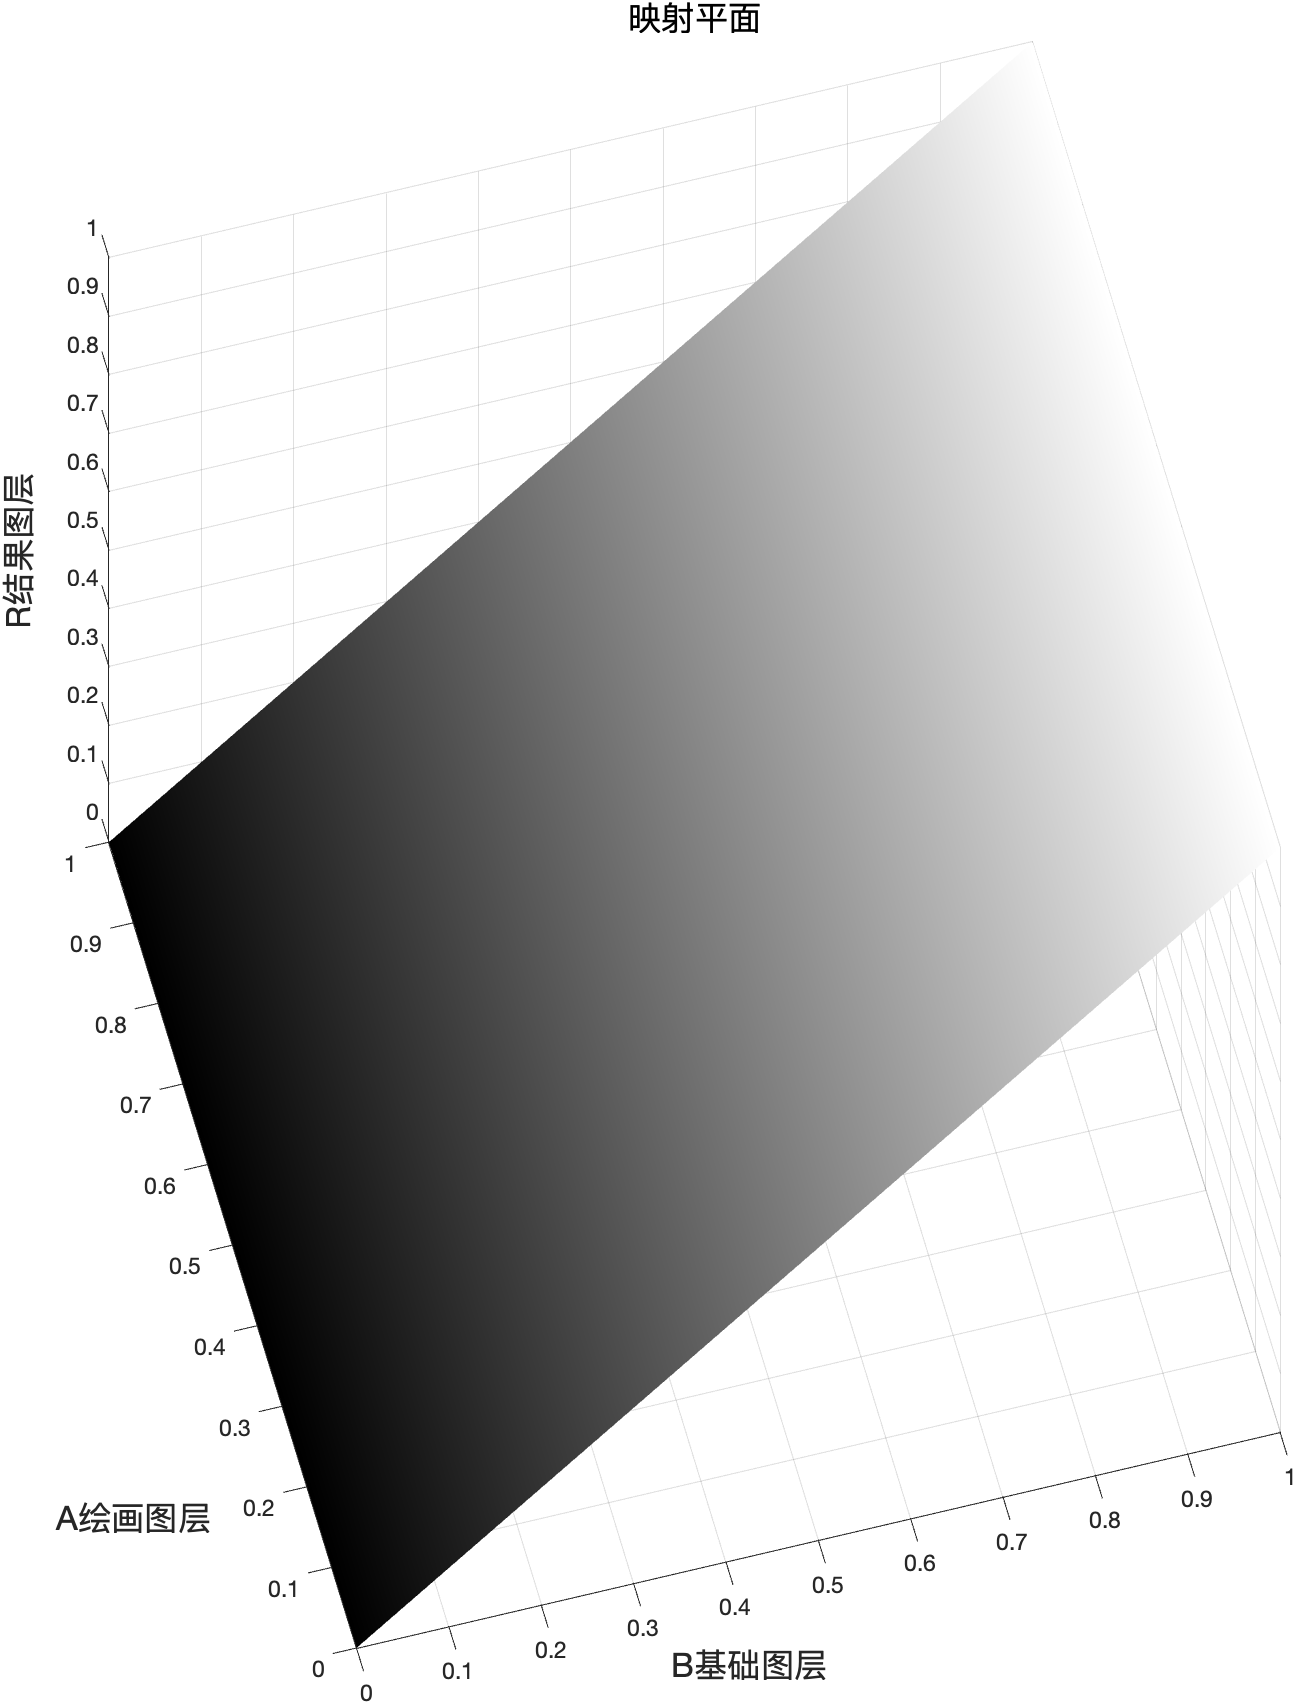
\includegraphics[width=0.5\textwidth]{01.png}
	\caption{映射面初始状态}
	\label{fig:initpic}
\end{figure}

\newpage
\subsection{ 映射面示例} 
映射面和原图面的对比 
使用混合模式后的映射面和原图映射面的对比
由图\ref{fig:initandnew}可以得知,这是一种变暗模式并且在混合图层和基础图层中选择了比较小的作为结果,因为可以明显看到一部分平面在原平面(图\ref{fig:initandnew}中的蓝色平面)的下方。
\begin{figure}[!htb]
	\centering
	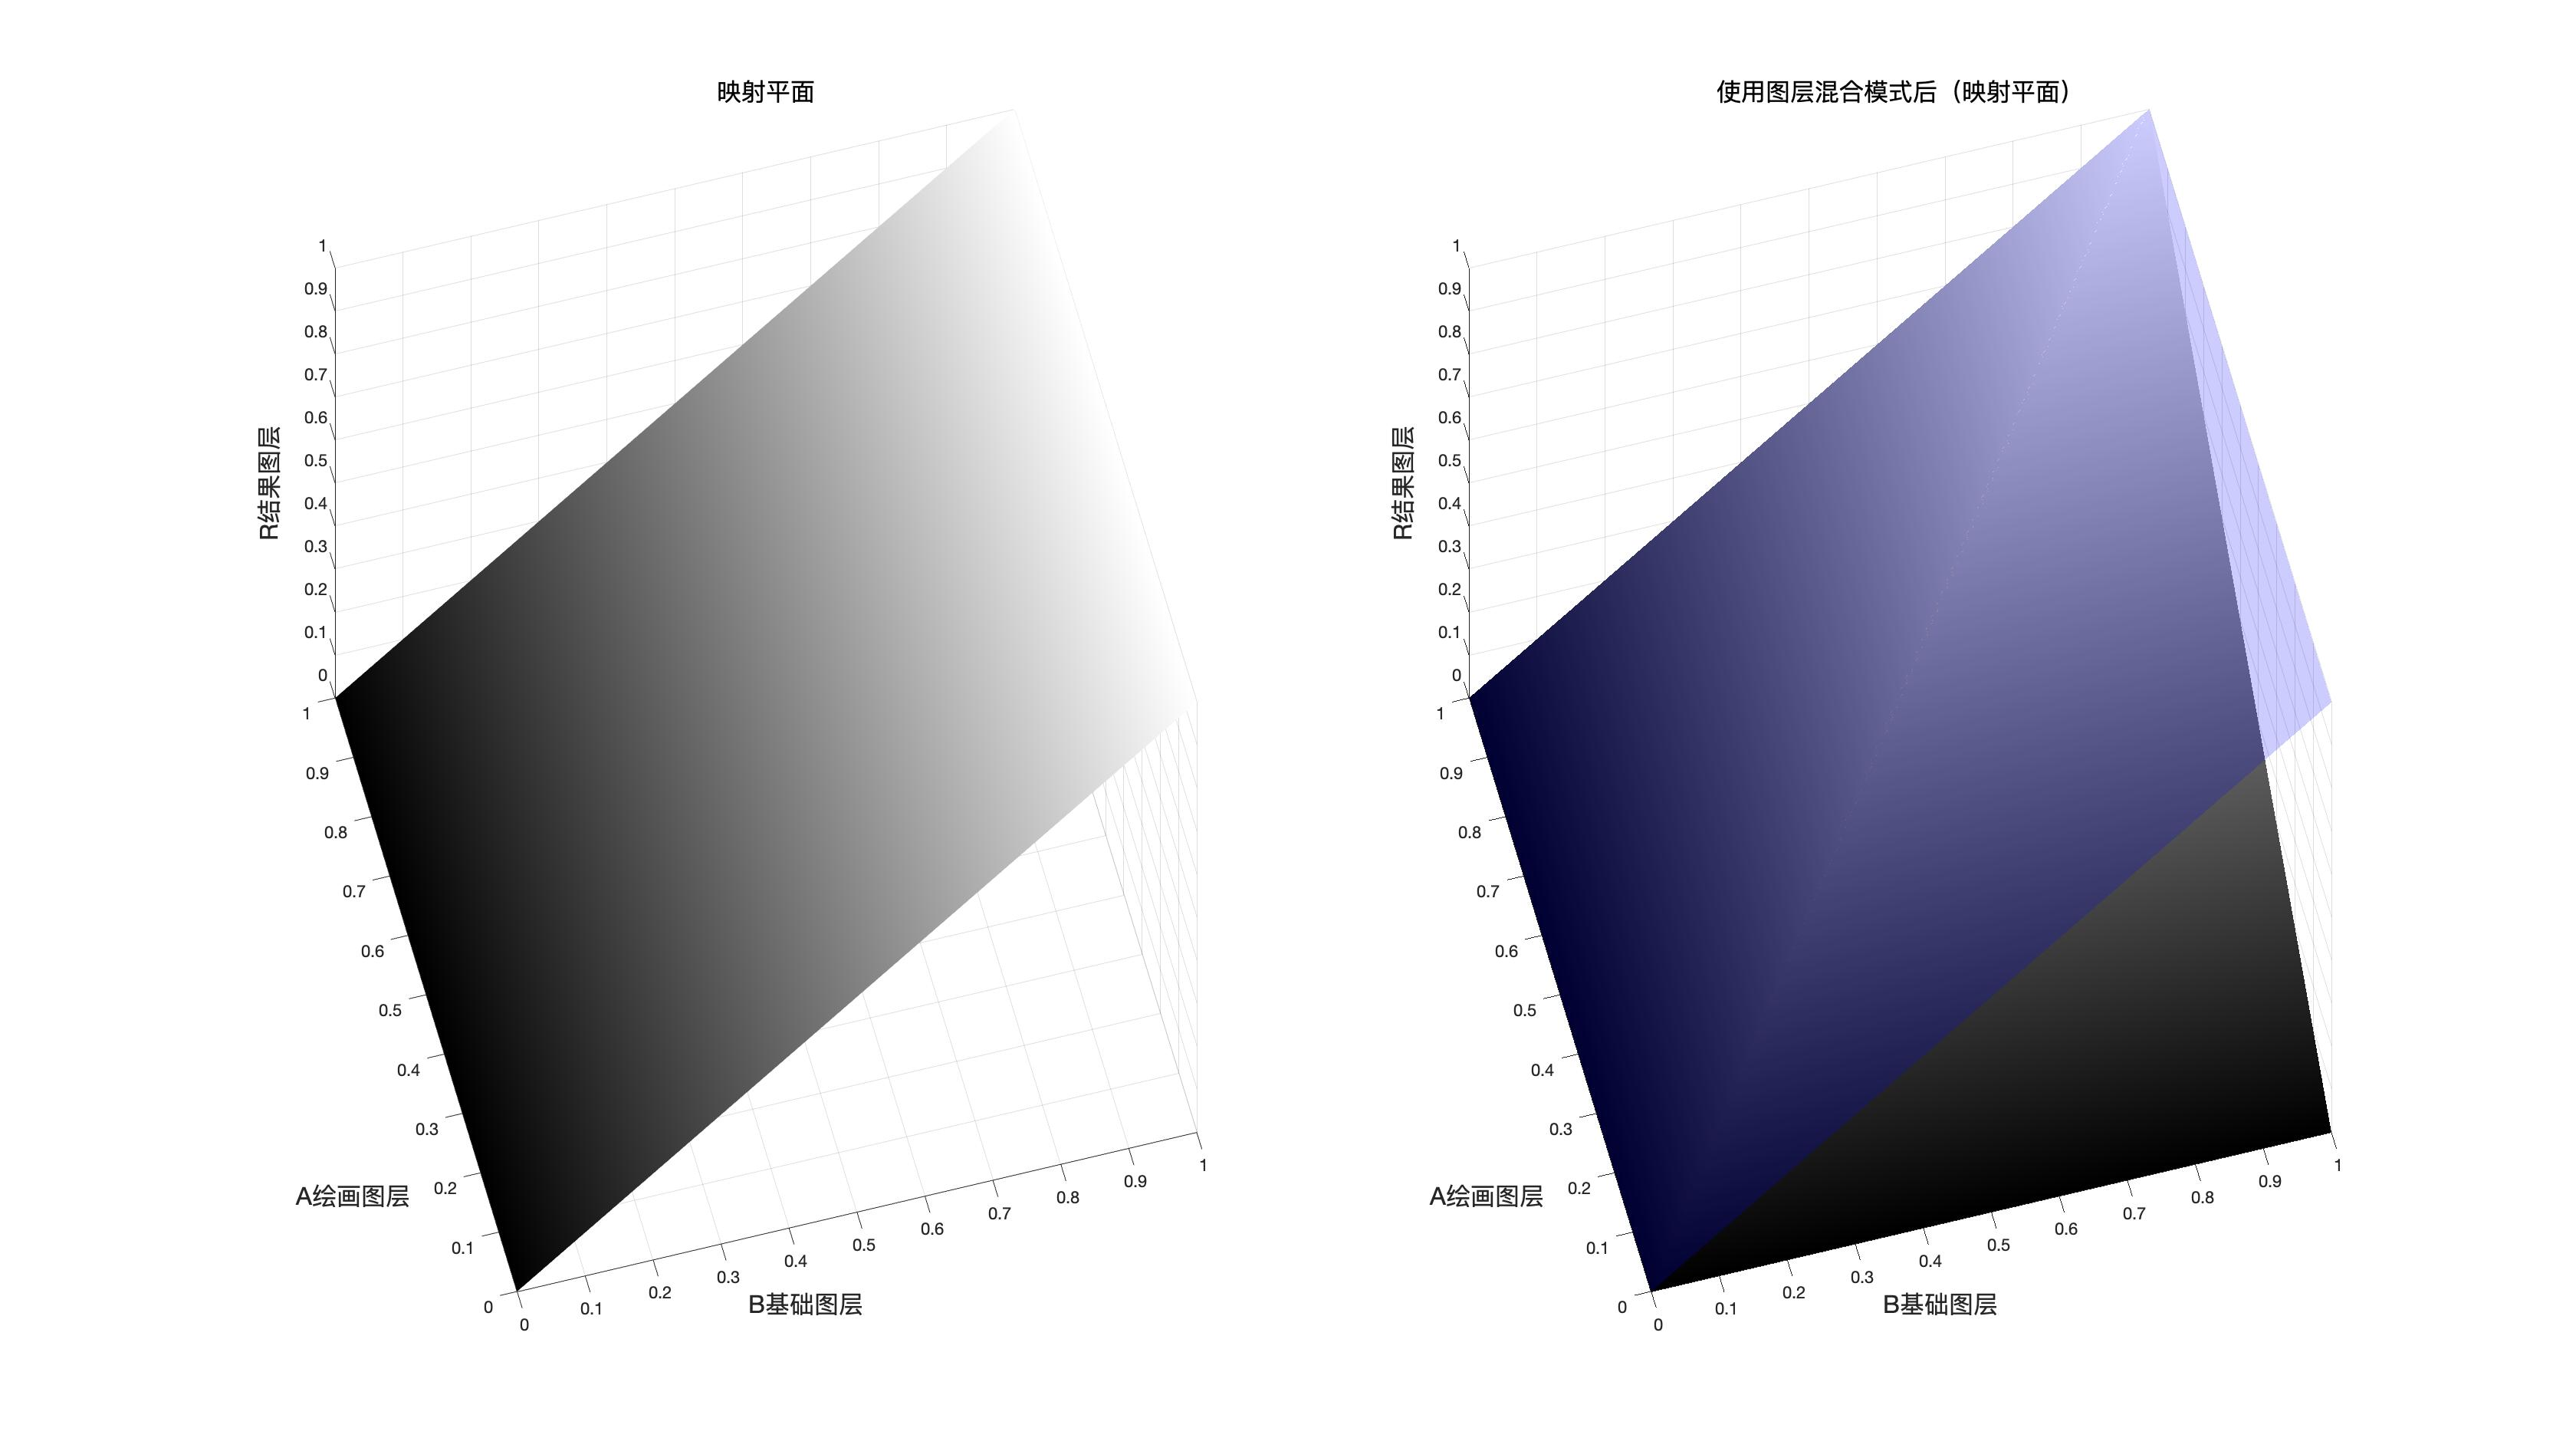
\includegraphics[width=\textwidth]{figure/映射面的引入}
	\caption{映射面和映射面初始状态对比}
	\label{fig:initandnew}
\end{figure}
\subsection{ 同图平面}
如果我们把基础图层和混合图层取值相同的点都标记出来,我们会得到一个对角平面,这个平面就是我们所说的同图平面 ,同图平面以及其和映射面相交的图像,图中绿色的平面就是同图平面,他和映射面的交线就是我们可以使用曲线工具模拟的曲线。如图\ref{fig:samepicsuf}所示。
% TODO: \usepackage{graphicx} required
\begin{figure}[!htb]
	\centering
	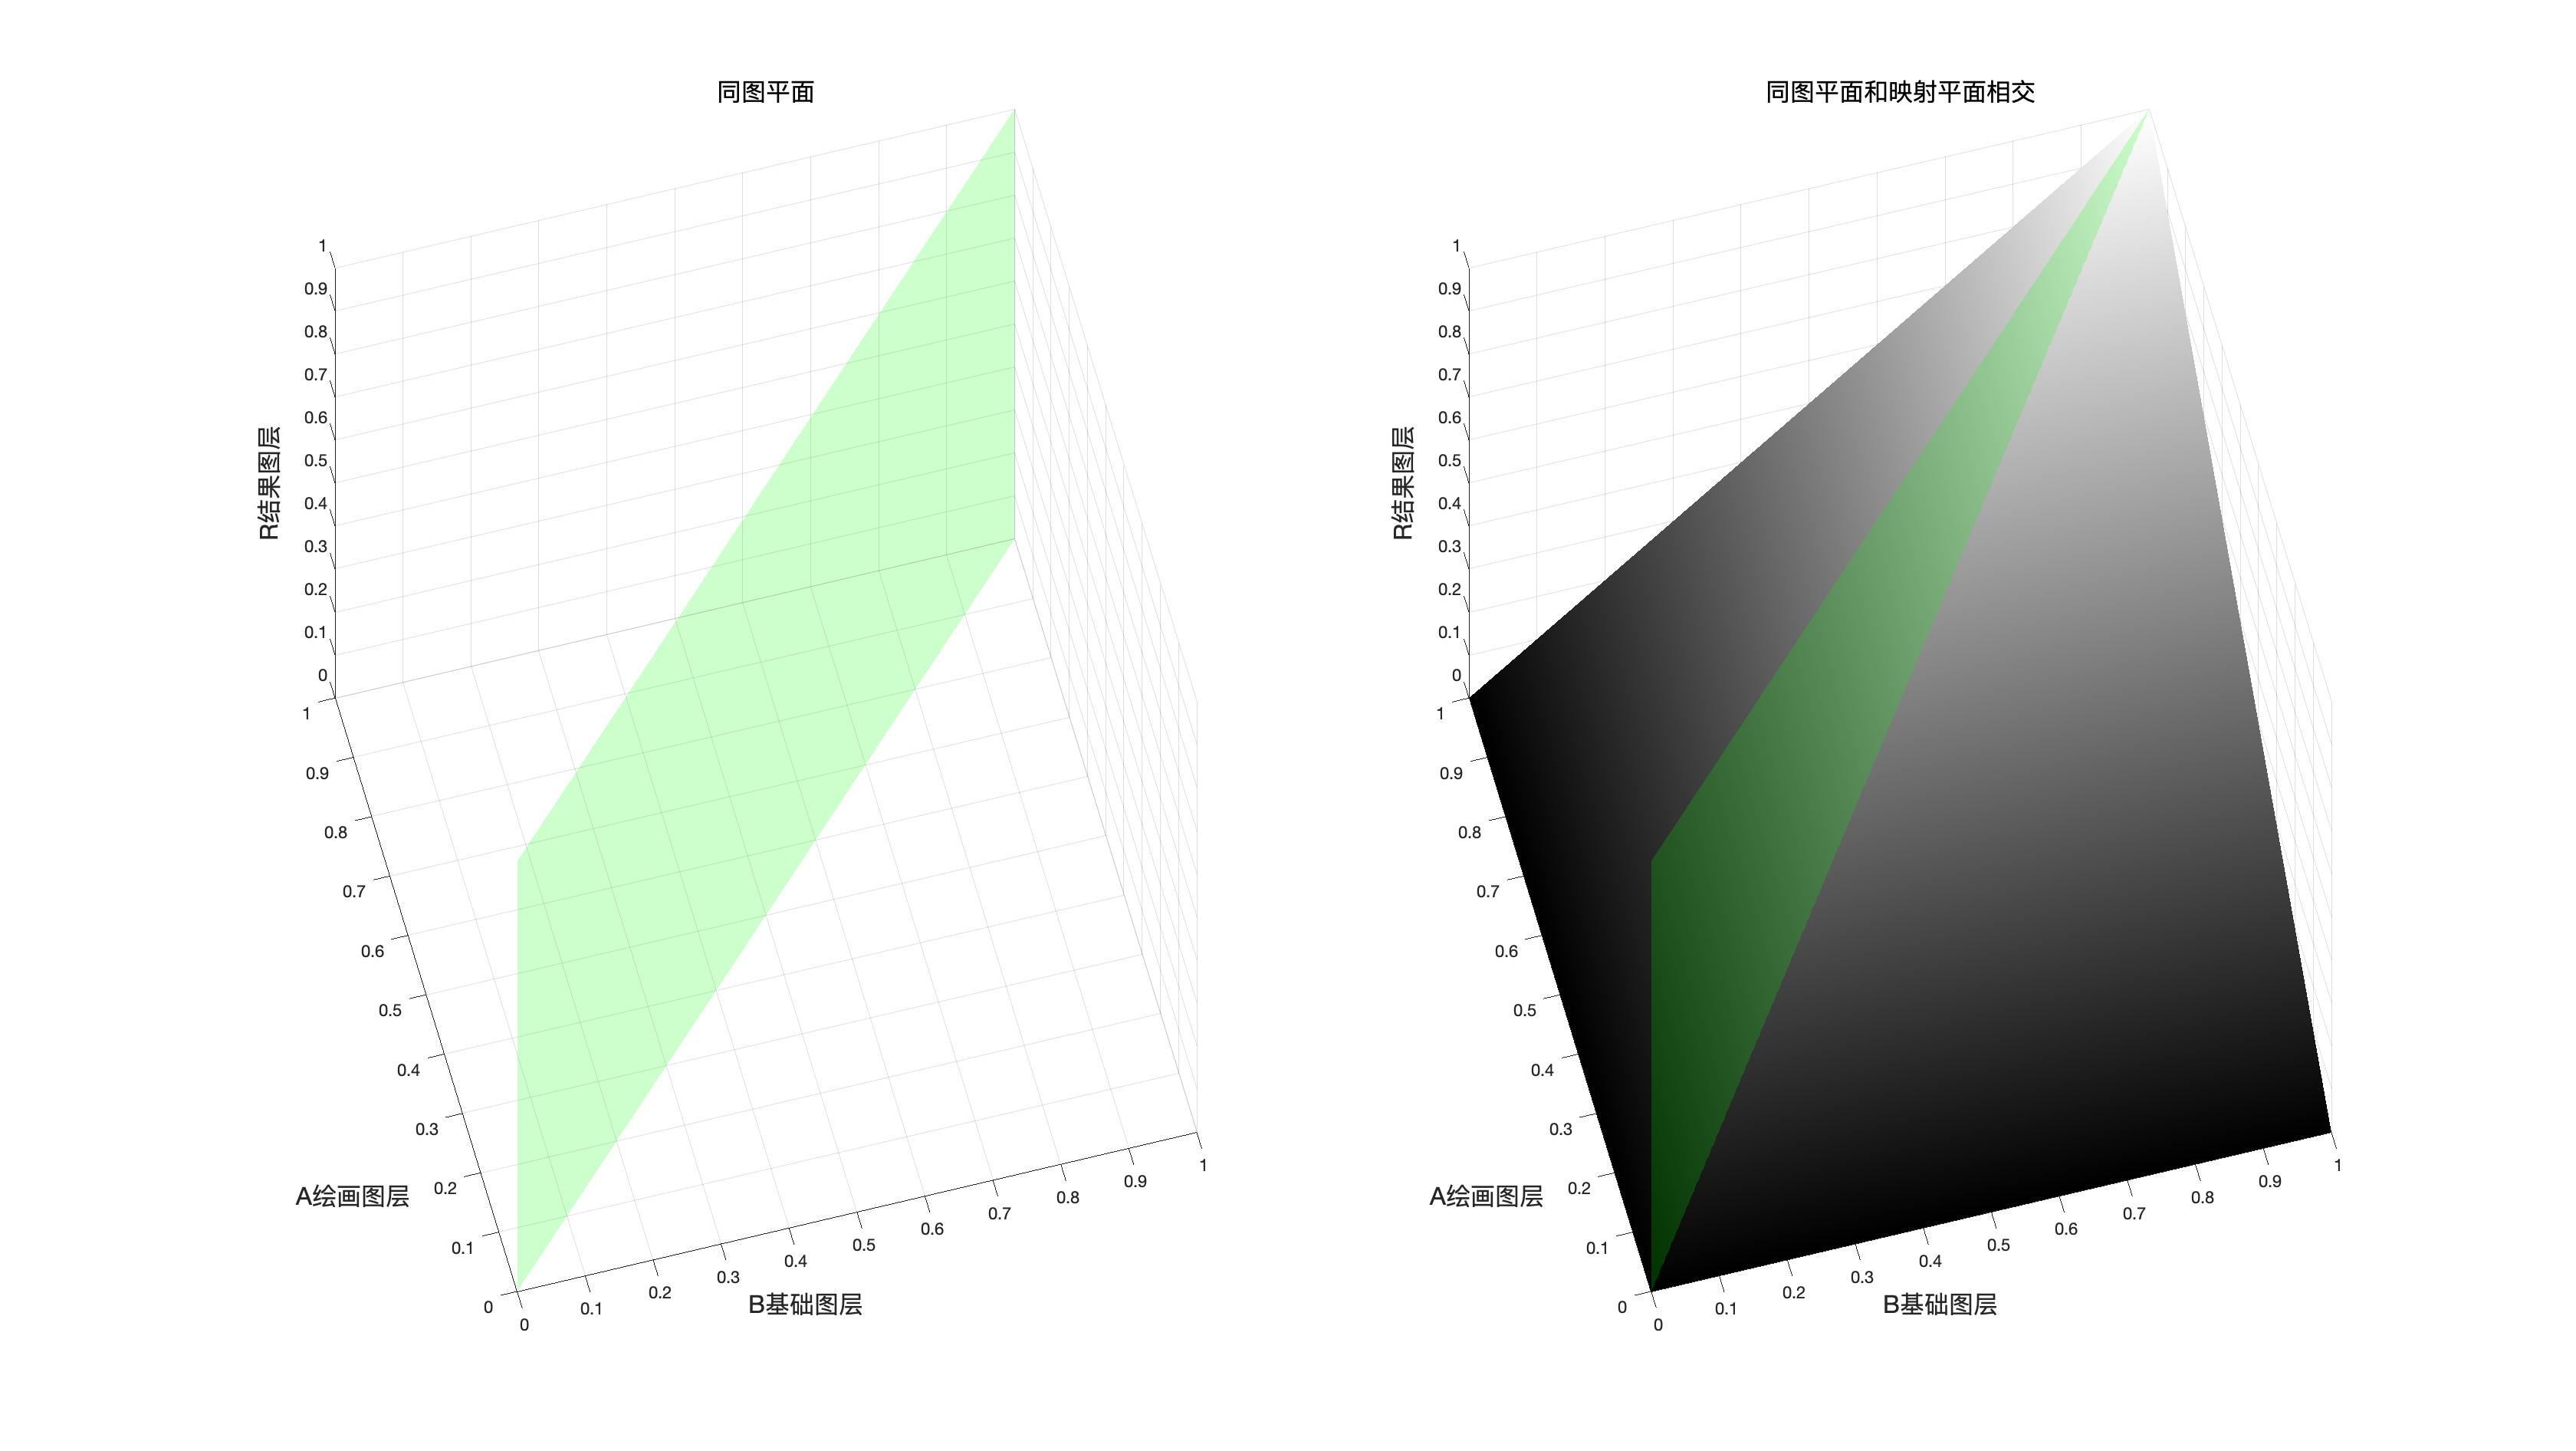
\includegraphics[width=\linewidth]{figure/同图平面}
	\caption{同图平面}
	\label{fig:samepicsuf}
\end{figure}

\subsection{ 同图混合曲线}
此时相当于$a=b$带入到某个图层混合模式的表达式中,我们此处以线性加深为例,线性加深原本的表达式是
\begin{equation}
	r=LinearBurn(b,a)=b-(1-a)=b+a-1
\end{equation}

若$b=a$则表达式可以写成
\begin{equation}
	\begin{aligned} r&=(b,b)=b-(1-b)\\&=b+b-1=2b-1\end{aligned}
\end{equation} 
% TODO: \usepackage{graphicx} required
\begin{figure}[!htb]
	\centering
	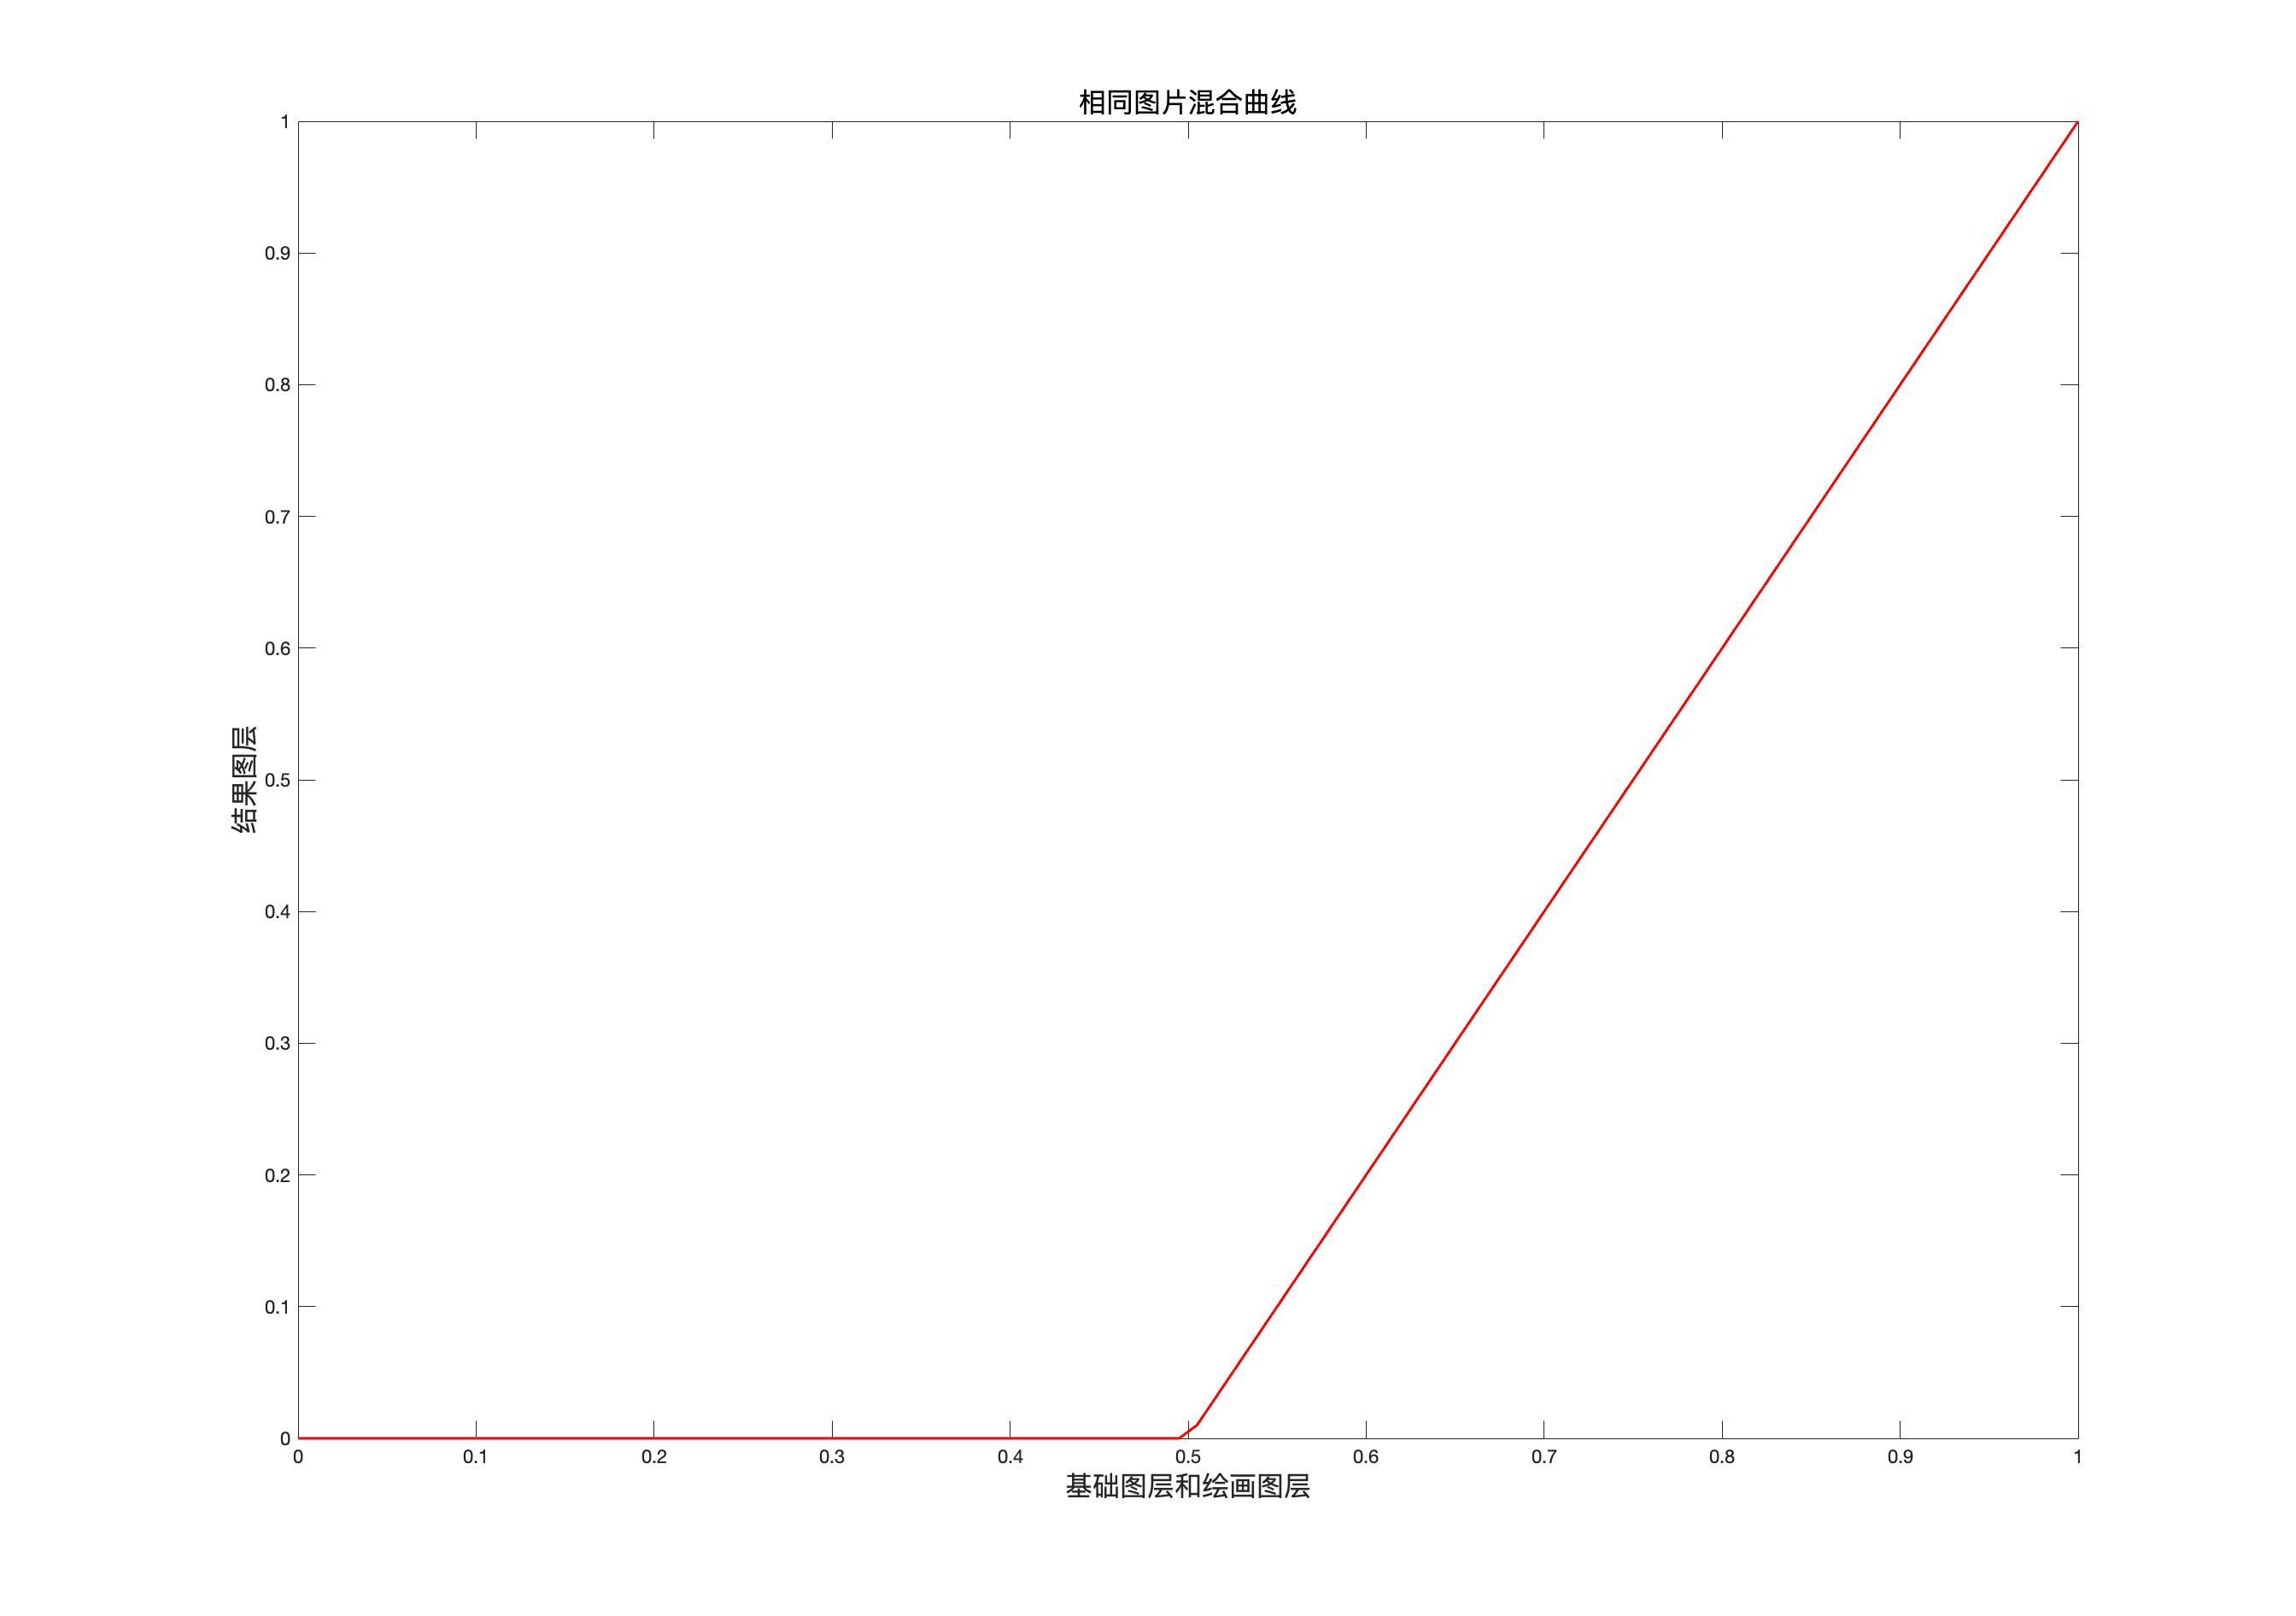
\includegraphics[width=0.7\linewidth]{figure/同图混合曲线示例}
	\caption{同图混合曲线示例}
	\label{fig:samepic}
\end{figure}

此时,在坐标系中画出该图像就如同上图所示。这时候我们只要打开曲线工具,然后拉一条曲线,和上图相同,就可以得到和这种混合模式在基础图层和混合图层相同的情况下的到结果图层相同的效果。

同图平面和映射面的交线就是可以使用曲线工具模拟这种混合模式时画出的曲线。同图平面有时候也可以作为分割平面,比如在实色混合模式的时候。

\subsection{ 中性灰平面}
如果我们把基础图层或者绘画图层中$128$中性灰的点都标记出来,我们会得到一个中性灰平面
这个平面一般作为结合两种混合模式的分割面
\subsubsection{ 基础图层的中性灰平面}
如果两种混合模式是以基础图层的取值作为分界依据的时候,使用此平面作为分割和结合依据。 如图\ref{fig:basemidgray}所示。

\begin{figure}[!htb]
	\centering
	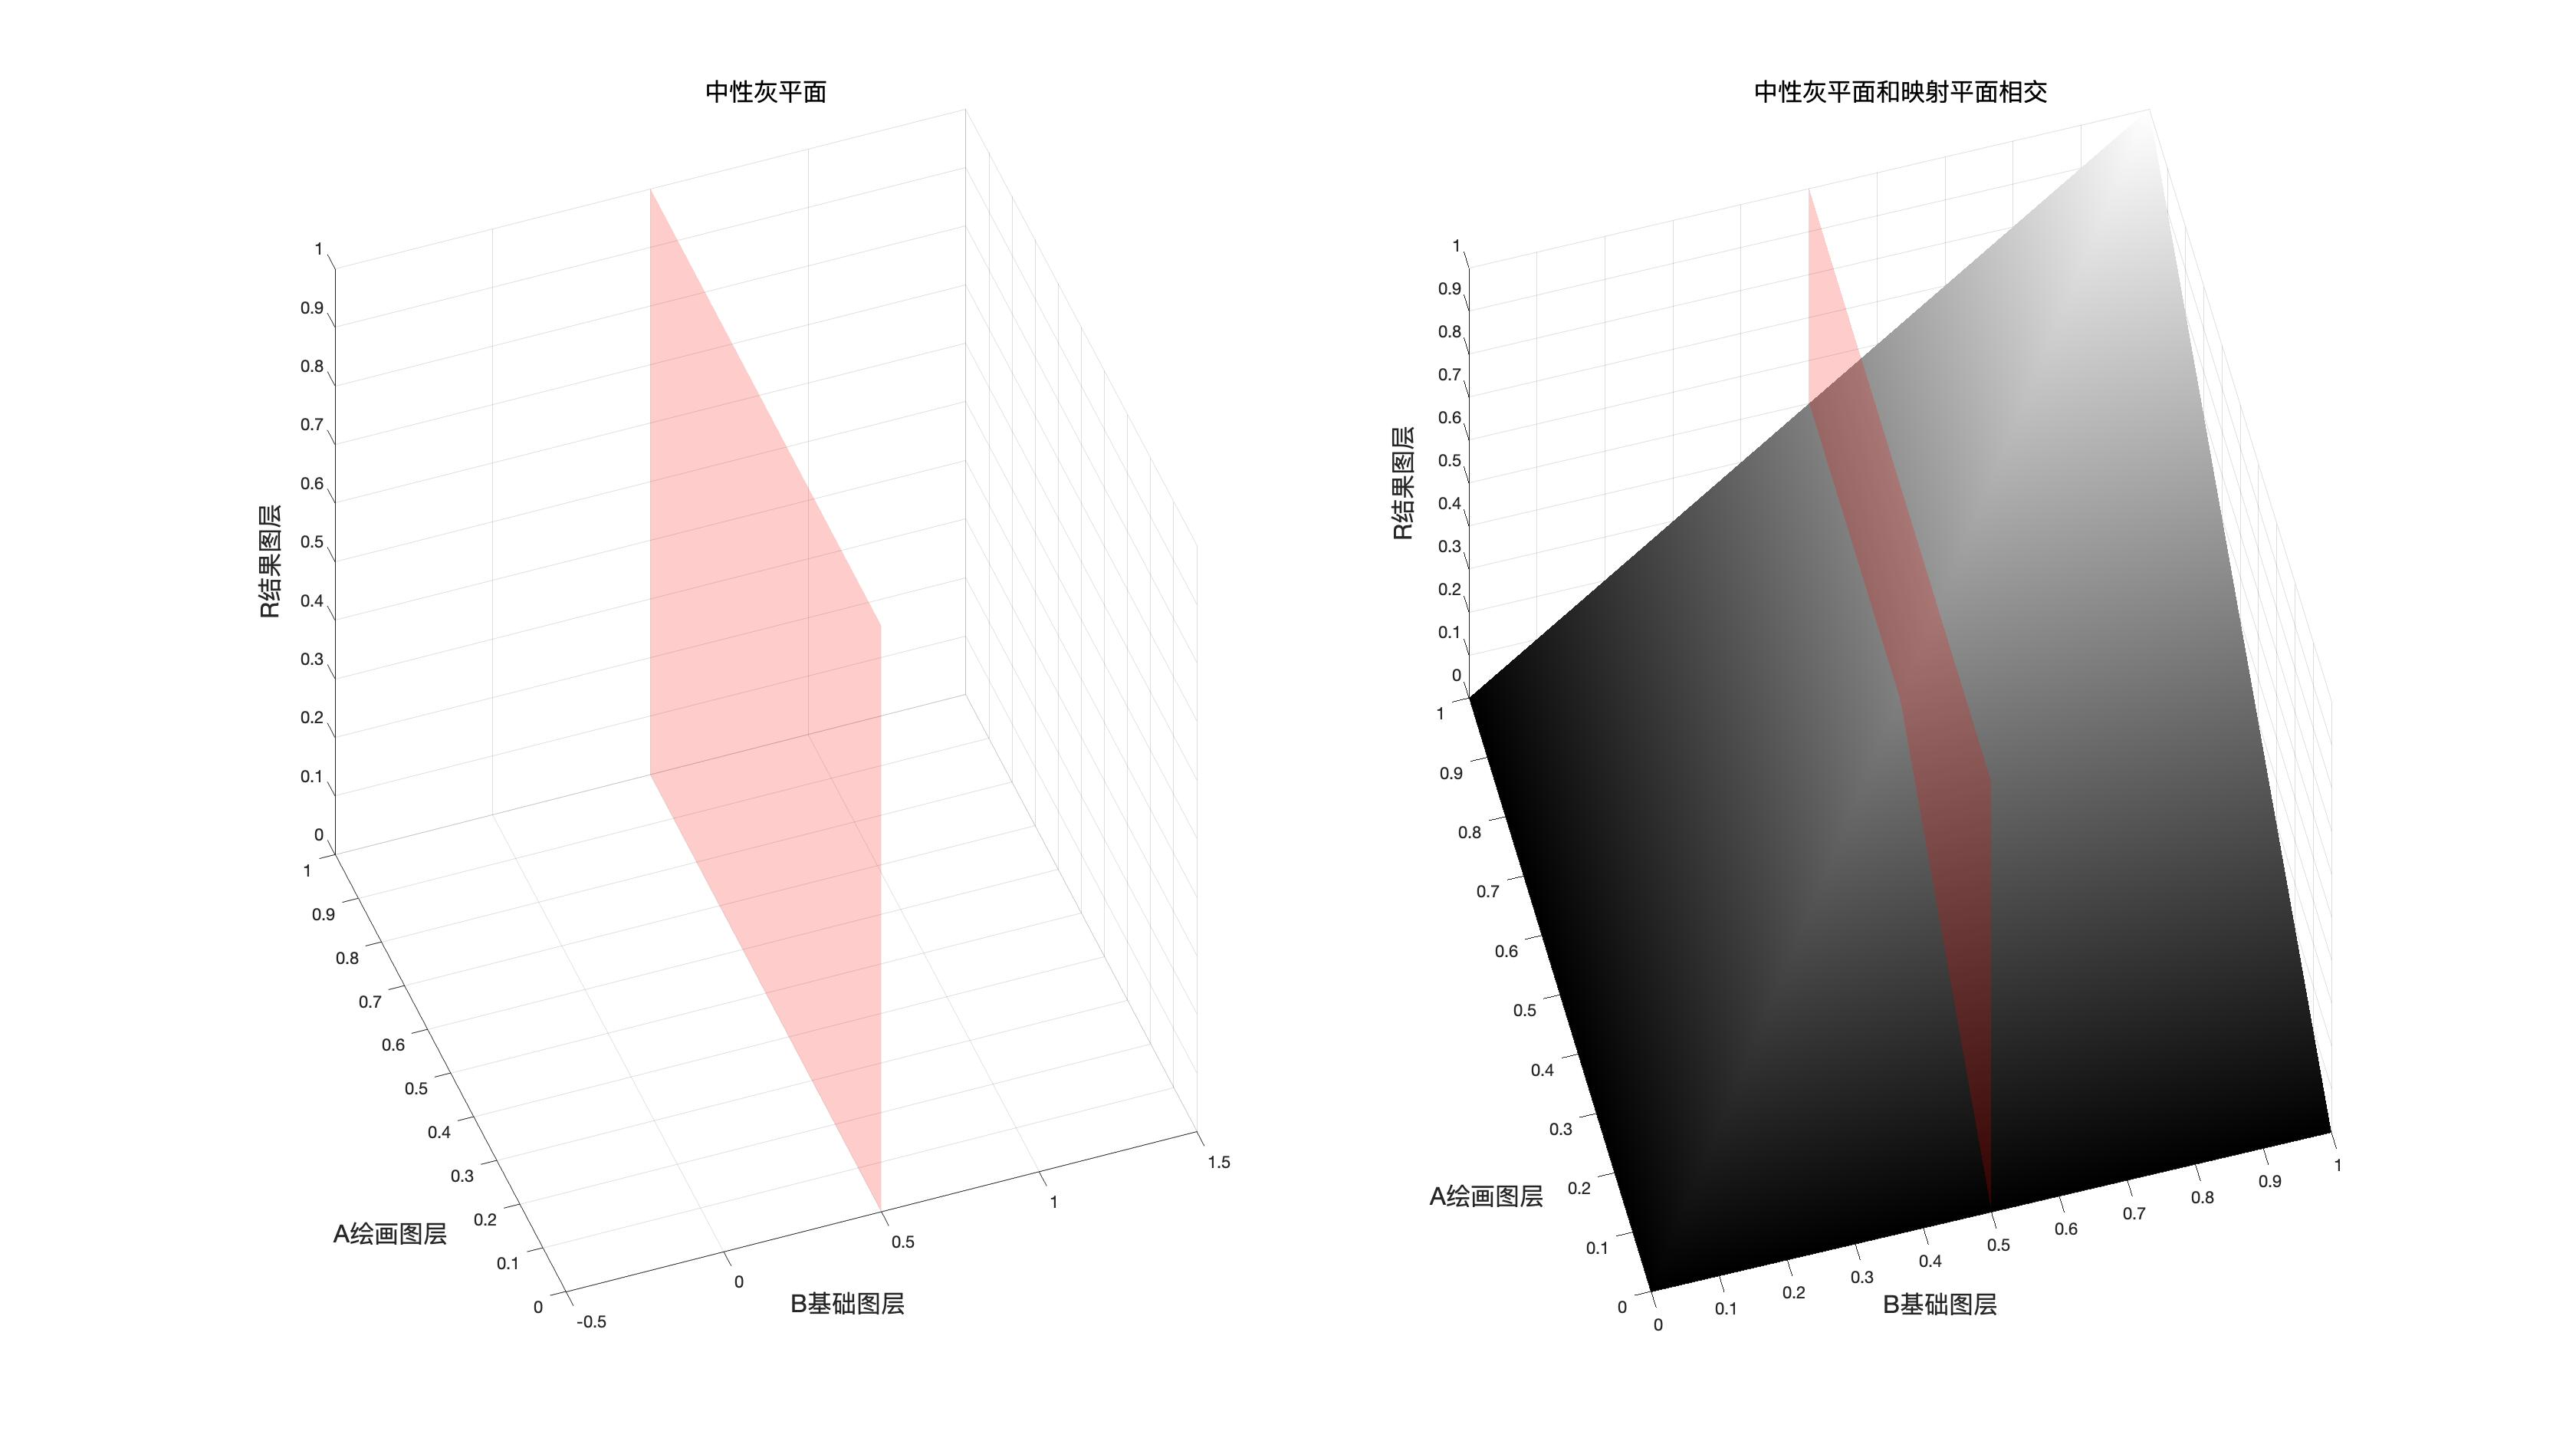
\includegraphics[width=\textwidth]{中性灰平面和映射平面相交.jpg}
	\caption{基础图层的中性灰平面}
	\label{fig:basemidgray}
\end{figure}
\subsubsection{ 混合图层的中性灰平面}
如果两种混合模式是以混合图层的取值作为分界依据的时候,使用此平面作为分割和结合依据。
同图平面,中性灰平面(基础中性灰平面,混图层中性灰平面)都是结合两种混合模式的依据。如图\ref{fig:blendmidgray}所示。
% TODO: \usepackage{graphicx} required
\begin{figure}[!htb]
	\centering
	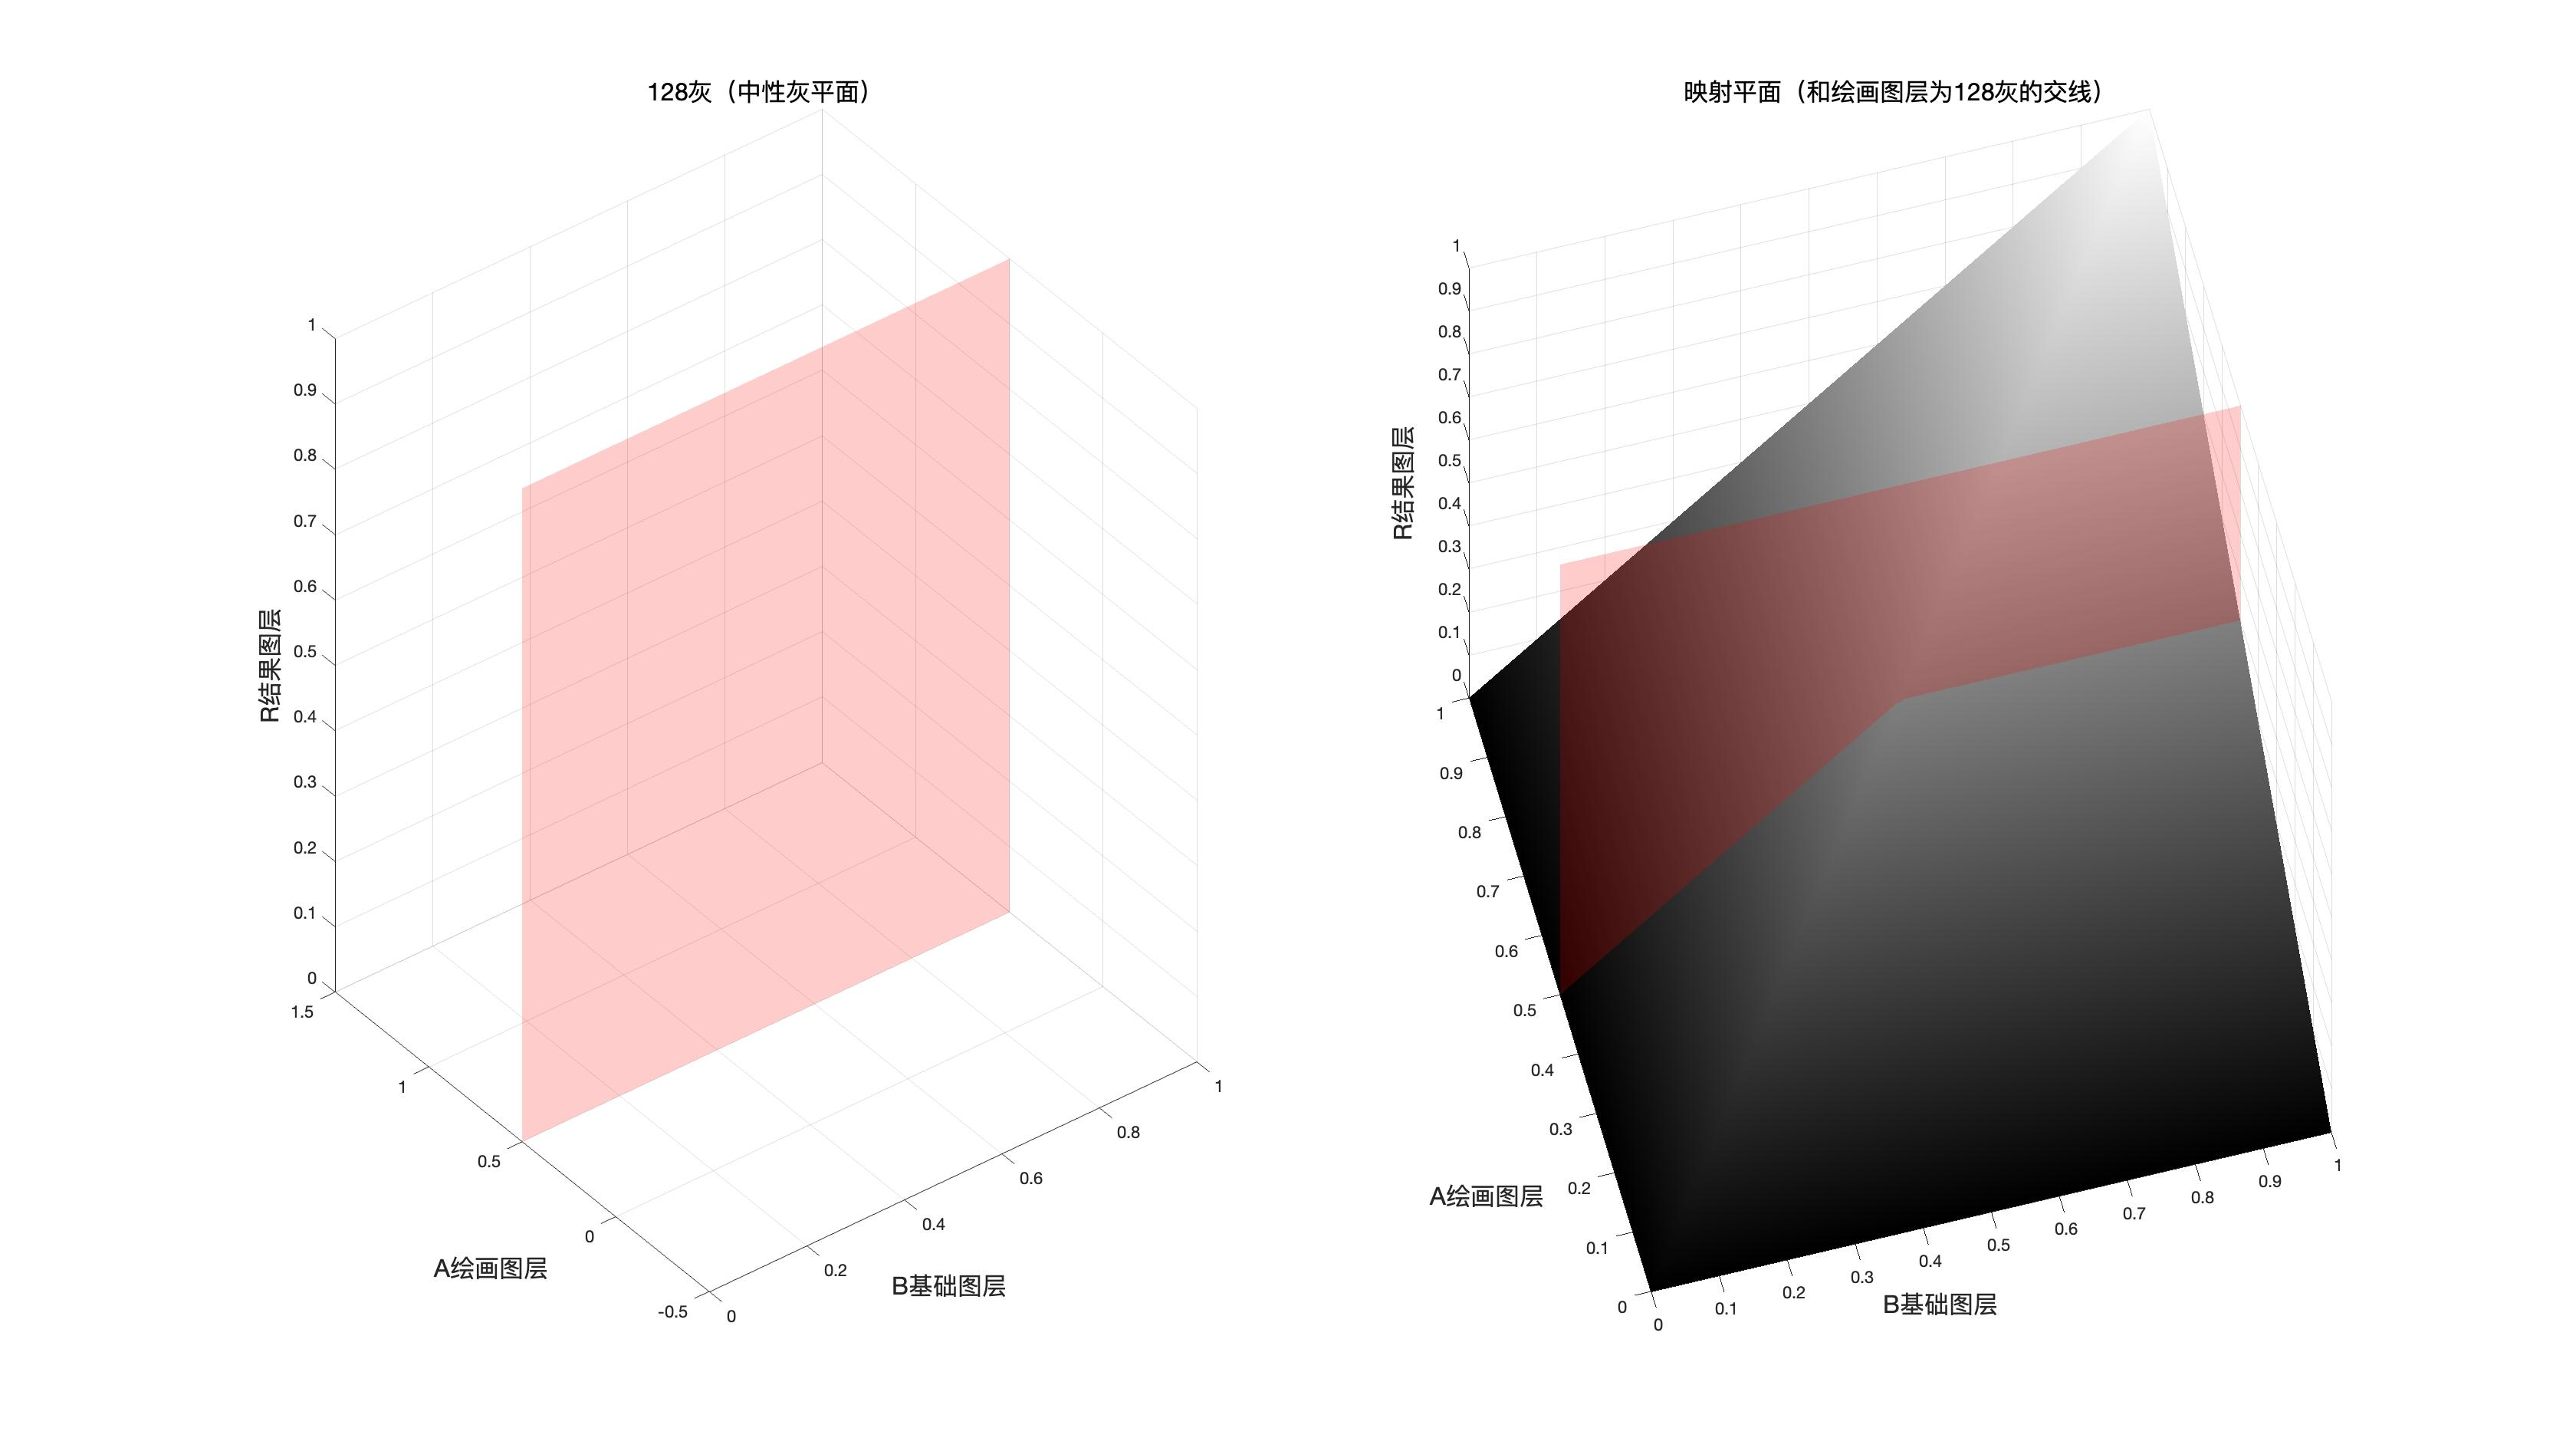
\includegraphics[width=\linewidth]{figure/中性灰和映射平面2}
	\caption{混合图层的中性灰平面}
	\label{fig:blendmidgray}
\end{figure}
\newpage
\section{ 关系总揽}
为了方便大家理解,我们在此给出27中图层混合模式的总览 ,如图\ref{fig:all}所示。

\begin{itemize}
	\item 可转换:代表两种混合模式可以在一定条件下等效另外一种
	\item 可交换:底图和绘画图层交换,两种混合模式产生的结果相同,也就是互逆
	\item 组成:一种混合模式可以由另外几种组成
\end{itemize}

\subsection{ 特殊关系}
从总览那幅图我们可以得出一些有趣的结论,就是有的混合模式在结合一些操作之后,结果等价于另外一种,有的图层混合模式和另外一种是互逆的关系,有些可以组合,有些对黑色无效,有些对白色无效,有些对中性灰无效,总之,他们的一切都蕴含在了公式中,如果你想搞清楚,就仔细研究一下。
\subsection{ 可转换}
可转换可能有些在实际操作中有偏差,因为在计算过程中可能出现大于1或者小于0的情况,导致被取舍。以下都是理论存在的情况。
\begin{itemize}
	\item 变亮$\Leftrightarrow$变暗(三次负片)
	\item 滤色$\Leftrightarrow$正片叠底(三次负片)
	\item 线性减淡$\Leftrightarrow$线性加深(三次负片)
	\item 颜色减淡$\Leftrightarrow$颜色加深(三次负片)
	\item 浅色$\Leftrightarrow$深色(三次负片)
	\item 线性加深$\Leftrightarrow$减去(一次负片)
	\item 颜色减淡$\Leftrightarrow$划分(一次负片)
	\item 颜色加深$\Leftrightarrow$划分(两次负片)
\end{itemize}

\subsection{ 互逆(可交换)}
\begin{itemize}
	\item 叠加$\Leftrightarrow$强光
	\item 颜色$\Leftrightarrow$明度
	\item 实色混合$\Leftrightarrow$线性光(当实色混合填充设置为0.5也就是50\%)
\end{itemize}
\subsection{ 组成}
\begin{itemize}
	\item 叠加 $=$ 正片叠底$+$滤色
	\item 强光 $=$ 正片叠底$+$滤色
	\item 线性光 $=$线性加深$+$线性减淡
	\item 实色混合 $=$ 线性加深$+$线性减淡
	\item 亮光 $=$ 颜色加深$+$颜色减淡
	\item 点光 $=$ 变亮$+$变暗
	\item 柔光$=$系数2的伽马矫正 $+$ 系数为0.5的伽马矫正
\end{itemize}
%\subsection{ 另外五种} 
%	 1、穿透 2、背后 3、擦除 4、相加 5、相减
\begin{landscape}
	% TODO: \usepackage{graphicx} required
	\begin{figure}[!htb]
		\centering
		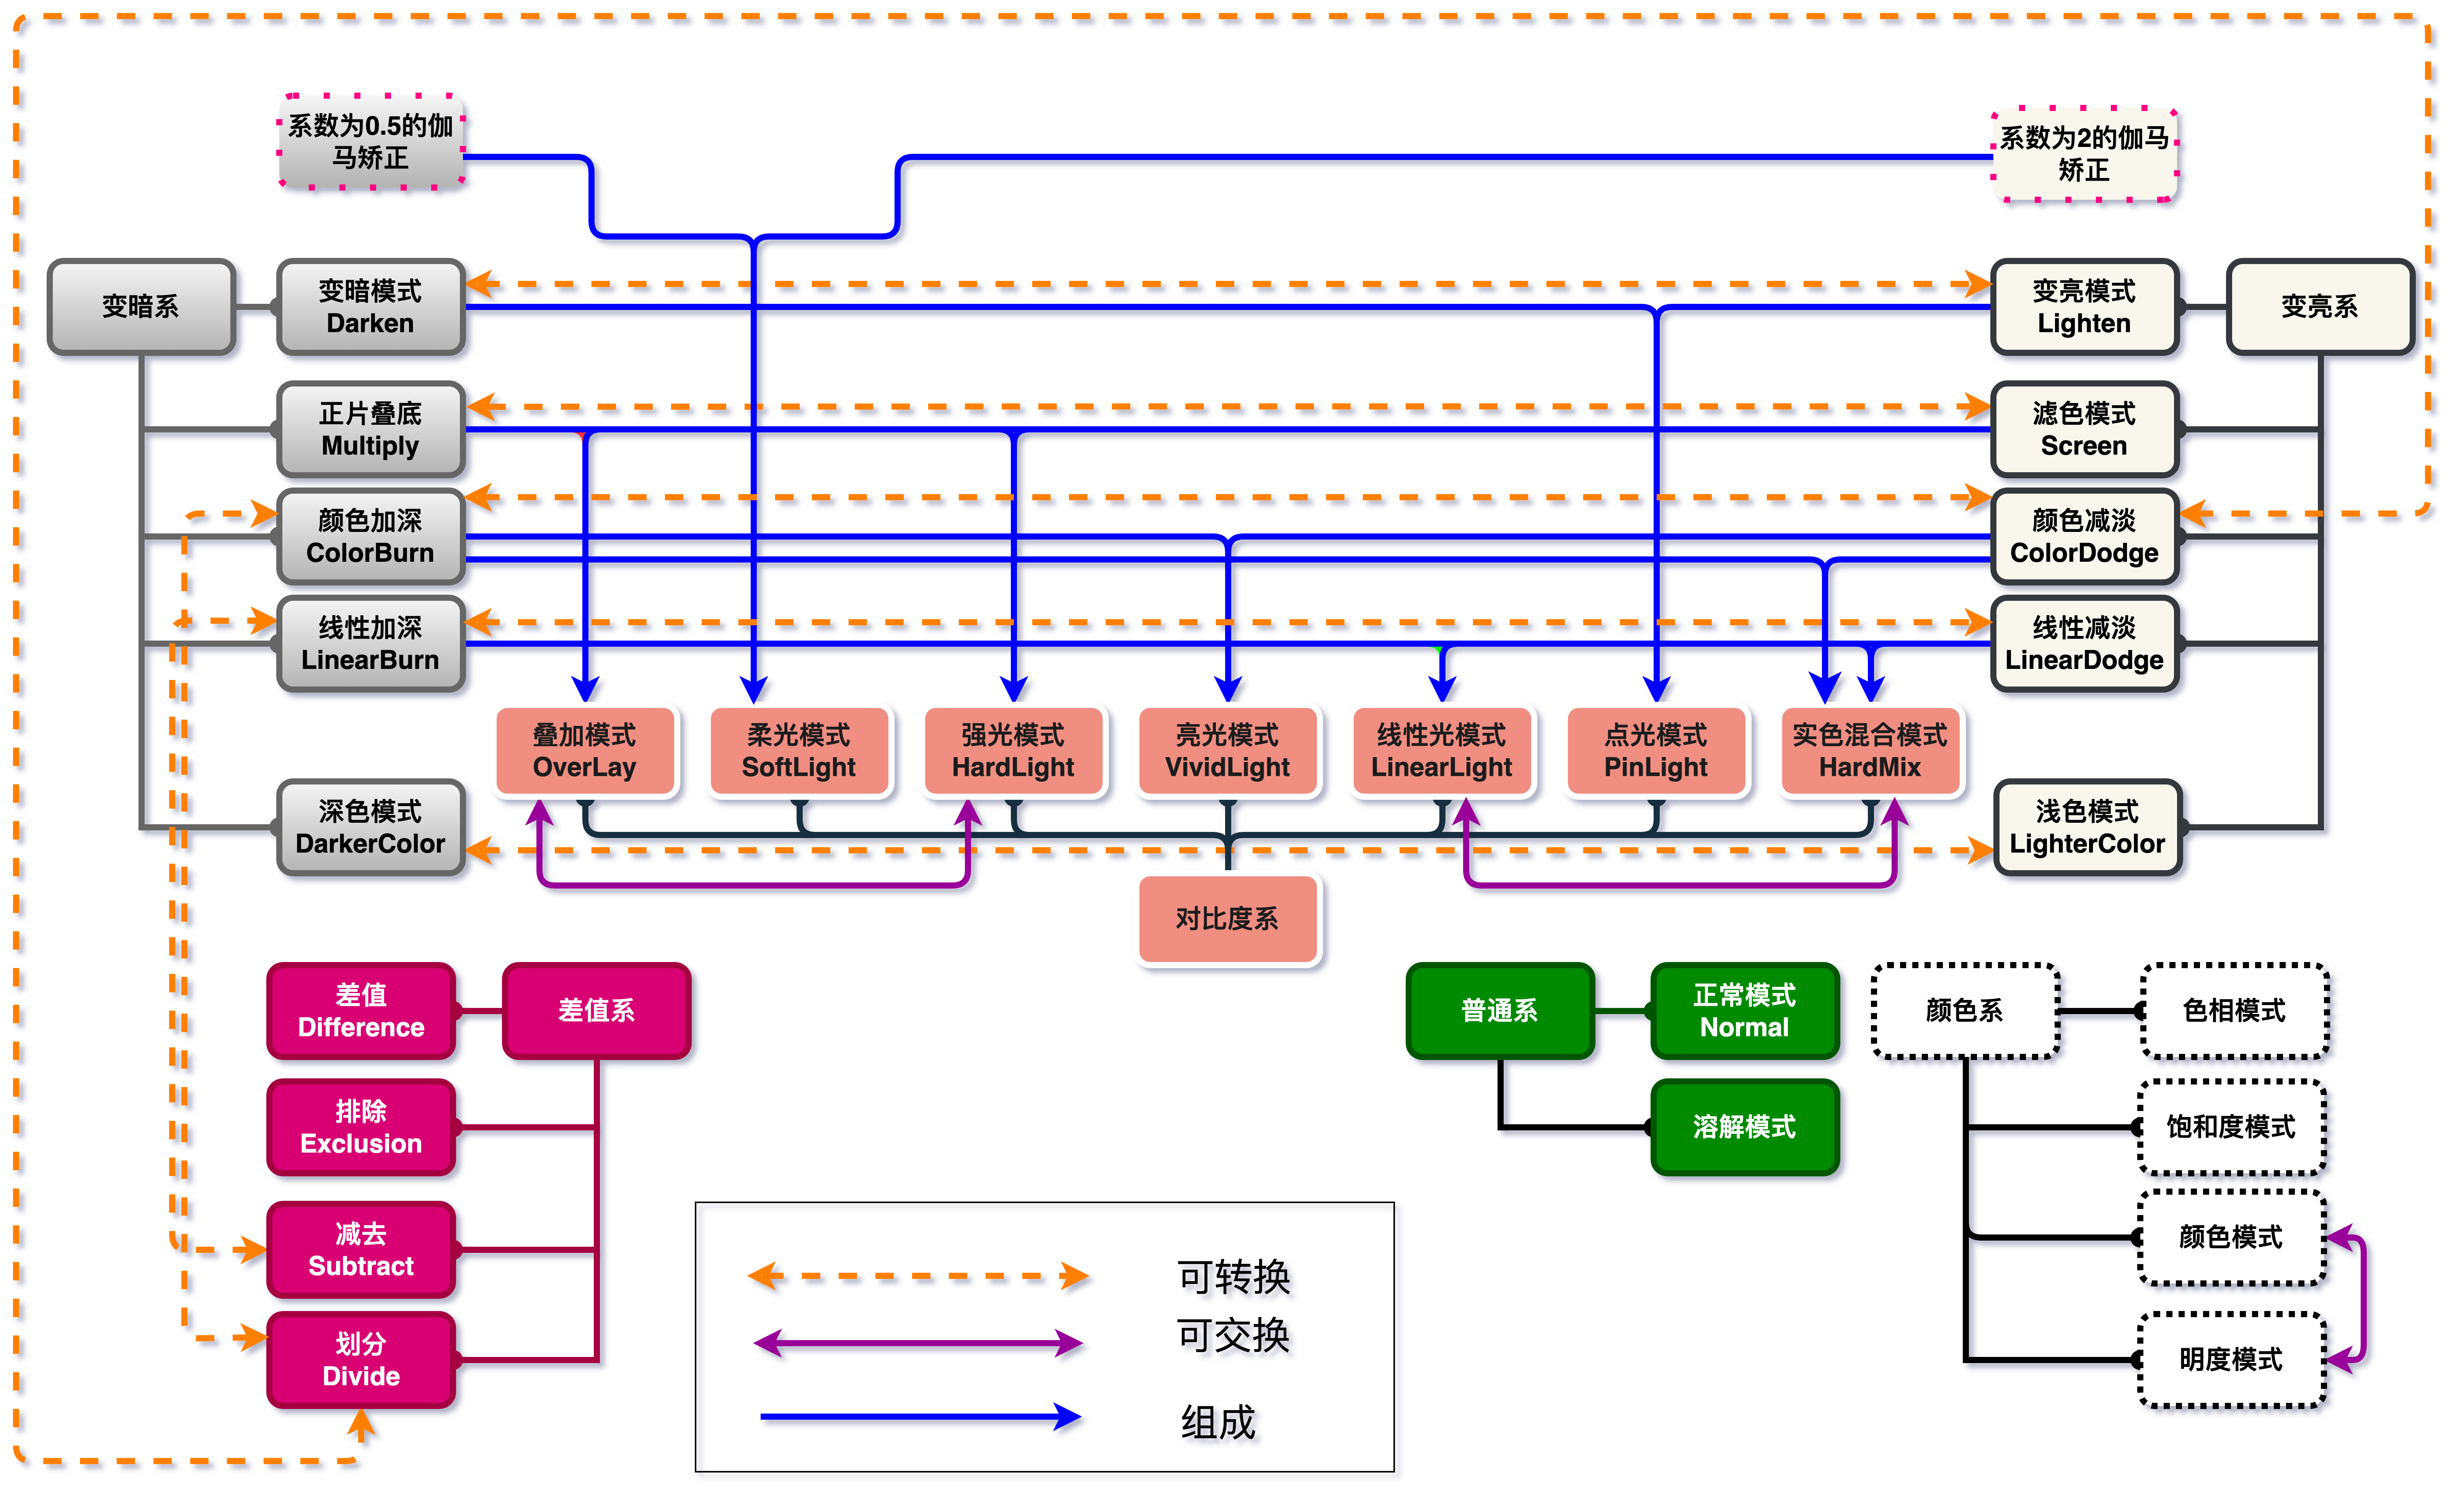
\includegraphics[width=\linewidth]{figure/全体}
		\caption{总览度}
		\label{fig:all}
	\end{figure}
\end{landscape}
\chapter{运算相关}
\begin{introduction}
	\item 本章包括图层混合模式需要知道的一切计算细节。
\end{introduction}
\section{ 归一化操作} 红色$(255,0,0)$,黑色$(0,0,0)$,白色$(255,255,255)$,中性灰色$(128,128,128)$。\newline
 如果我们对每个通道都用\textbf{归一化操作}。
 
 RC,GC,BC的取值范围都是$[0,255]$。
\begin{notice}
\item 此处我们使用线性归一化,具体方法是$$x'=\dfrac{x-min(x)}{max(x)-min(x)}$$在这里我们可以看到,最大值是255,最小值是0,于是上式可以简化为颜色值除以255
\end{notice}
\indent 以RC为例,$RC\in[0,255]$\newline
\indent 那我们可以得到归一化后\begin{equation}\dfrac{RC}{255}\Rightarrow rc\in [0,1]\end{equation}
\indent 那么以上的四种颜色就可以表示为,红色$(1,0,0)$,黑色$(0,0,0)$,白色$(1,1,1)$,中性灰色$(0.5,0.5,0.5)$。
\begin{equation}
	Pix= (RC,GC,BC)=(rc,gc,bc)
\end{equation}
\begin{notice}
	\item 这里也是为什么,在有些地方可以看到一堆255,一些地方看不到的原因。
\end{notice}

\section{ 一些运算规则}
如果一个图片的数值需要扩大或者缩小$x$倍
\subsection{通道级别}
通道数值乘以$x$
\[RC\times x \]
\subsection{ 像素级别}
如果一个像素点$Pix\times x$则表示其中所有通道数值都乘$x$,也就是说
\begin{equation}
Pix\times x = (RC\times x,GC\times x,BC\times x)
\end{equation}
\subsection{ 图层级别}
如果是图层$Layer\times x$则表示所有像素点都乘$x$
也就是说
\begin{equation}\begin{aligned}
&	Layer\times x=\left\{ \begin{aligned}     &Pix_{(1,1)}\times x&&\cdots&&Pix_{(1,n)}\times x\\&\vdots && &&\vdots\\  &Pix_{(1,n)}\times x &&\cdots&&Pix_{(i,n)}\times x\\&\vdots && &&\vdots\\  &Pix_{(m,1)}\times x &&\cdots&&Pix_{(m,n)}\times x\\  \end{aligned}\right\}\\\\&=\left\{ \begin{aligned}     &(RC_{(1,1)}\times x,GC_{(1,1)}\times x,BC_{(1,1)}\times x)&&\cdots&&(RC_{(1,n)}\times x,GC_{(1,n)}\times x,BC_{(1,n)}\times x)\\&\vdots && &&\vdots\\  &(RC_{(1,n)}\times x,GC_{(1,n)}\times x,BC_{(1,n)}\times x) &&\cdots&&(RC_{(i,n)}\times x,GC_{(i,n)}\times x,BC_{(i,n)}\times x)\\&\vdots && &&\vdots\\  &(RC_{(m,1)}\times x,GC_{(m,1)}\times x,BC_{(m,1)}\times x) &&\cdots&&(RC_{(m,n)}\times x,GC_{(m,n)}\times x,BC_{(m,n)}\times x)\\  \end{aligned}\right\}
\end{aligned}\end{equation}

\begin{notice}
	\item 一般我们说底图减去混合图层,或者,基础图层和混合图层使用混合模式,都将这些级别的运算包含在了一句简单的表述中。
\end{notice} 
\subsection{HSY的运算}
如果是HSY的色彩空间,那么我们的表达式其实和RGB的没有什么区别,如果非要说区别,就是我们需要把像素的表达式稍微变一下。一般HSY空间只涉及交换,而不涉及运算。
\section{ 混合模式相关符号}
\indent 图层混合模式我们使用$BlendMode$来表示,这里是一个泛指,如果涉及到具体的混合模式,有专门的表示符号,比如正常模式使用$Normal$
使用矩阵我们有:
\begin{equation}
	\text{基础图层}\Longleftrightarrow LayerA=\left\{ \begin{aligned}     &PixA_{(1,1)}&&\cdots&&PixA_{(1,n)}\\&\vdots && &&\vdots\\  &PixA_{(i,1)} &&\cdots&&PixA_{(i,n)}\\&\vdots && &&\vdots\\  &PixA_{(m,1)} &&\cdots&&PixA_{(m,n)}\\  \end{aligned}\right\}
\end{equation}
\begin{equation}\text{混合图层}\Longleftrightarrow LayerB=\left\{ \begin{aligned}     &PixB_{(1,1)}&&\cdots&&PixB_{(1,n)}\\&\vdots && &&\vdots\\  &PixB_{(i,1)} &&\cdots&&PixB_{(i,n)}\\&\vdots && &&\vdots\\  &PixB_{(m,1)} &&\cdots&&PixB_{(m,n)}\\ \end{aligned}\right\}\end{equation}
\begin{equation}\text{结果图层}\Longleftrightarrow LayerR=\left\{ \begin{aligned}     &PixR_{(1,1)}&&\cdots&&PixR_{(1,n)}\\&\vdots && &&\vdots\\  &PixR_{(i,1)} &&\cdots&&PixR_{(i,n)}\\&\vdots && &&\vdots\\  &PixR_{(m,1)} &&\cdots&&PixR_{(m,n)}\\ \end{aligned}\right\}\end{equation}

再结合上面的三者关系公式
\begin{equation}\begin{aligned}
	\text{结果图层}&=BlendMode(\text{基础图层},\text{混合图层})\\\Updownarrow\\LayerR&=BlendMode(LayerB,LayerA)
	\end{aligned}\end{equation}

我们得到
\begin{equation}LayerR=\left\{ \begin{aligned}   &BlendMode(PixB_{(1,1)},PixA_{(1,1)})&&\cdots&&BlendMode(PixB_{(1,n)},PixA_{(1,n)})\\&\vdots && &&\vdots\\&BlendMode(PixB_{(i,1)},PixA_{(i,1)})&&\cdots&&BlendMode(PixB_{(i,n)},PixA_{(i,n)})\\&\vdots && &&\vdots\\&BlendMode(PixB_{(m,1)},PixA_{(m,1)})&&\cdots&&BlendMode(PixB_{(m,n)},PixA_{(m,n)})\\\end{aligned}\right\}\end{equation}

\indent 对于其中任意项
\begin{equation}
	Pix_R=BlendMode(Pix_B,Pix_A)
\end{equation}

 如果这种混合模式基于RGB色彩空间则
上述表达式可以写为

\begin{equation}
	(rc_{R},gc_{R},bc_{R})=BlendMode((rc_{B},gc_{B},bc_{B}),(rc_{A},gc_{A},bc_{A}))
\end{equation}

或者未归一化形式
\begin{equation}
	(RC_{R},GC_{R},BC_{R})=BlendMode((RC_{B}, GC_{B}, BC_{B}),(RC_{A}, GC_{A}, BC_{A}))
\end{equation}

如果这种混合模式基于HSY色彩空间
\begin{equation}
	(H_{R},S_{R},Y_{R})=BlendMode((H_{B},S_{B},Y_{B}),(H_{A},S_{A},Y_{A}))
\end{equation}

\begin{notice}
	\item 在下面的所有组中,如果不特别说明基于RGB色彩空间的混合模式都是使用归一化后的数值进行计算。并且,为了方便大家验证计算的正确性,这里提供一个java程序的链接给各位,GitHub的地址如下,输入你要混合的像素的数值,就可以得到对应混合模式混合的结果数值。
\end{notice} 
\newpage
\section{ 辅助计算程序}
为了辅助我们计算并且验证这些理论公式和PS中实际运行的结果是否一致,我们借助java代码来实现具体的计算过程,手动计算可以,但是浪费时间,我们有更简单的方式。我们定义一个java类BlendColor,这个类用RGB作为基础,每次计算都以RGB存储,如果需要其他表达式,则我们通过RGB转换。


\begin{lstlisting}
	public class BlendColor {
		public ColorItem red;
		public ColorItem green;
		public ColorItem blue;
		public List<ColorItem> orderColorList;
		
		public BlendColor(double redv, double greenv, double bluev) {
			ColorItem red = new ColorItem("red", redv);
			ColorItem green = new ColorItem("green", greenv);
			ColorItem blue = new ColorItem("blue", bluev);
			this.orderColorList = new ArrayList<ColorItem>();
			this.red = red;
			this.green = green;
			this.blue = blue;
			this.orderColorList.add(red);
			this.orderColorList.add(green);
			this.orderColorList.add(blue);
			// 排序
			Collections.sort(this.orderColorList);
		}
		...
	}
\end{lstlisting}


\section{ 混合模式的组合}
一般来说,混合模式的组合会以基础图层B或者混合图层A的中性灰分割线为界,组合两种不同的混合模式。例如,强光模式,它是由正片叠底和滤色两种模式以混合图层的中性灰分割线为界完成组合

\begin{itemize}
	\item 正片叠底$r=Multiply(b,a)=b\times a$
	\item 滤色$r=Screen(b,a)=1-(1-b)(1-a)$
	\item 强光\begin{equation}
		\begin{aligned}
			r&=HardLight(b,a)=\left\{ \begin{aligned}&Multiply(b,2a)&a\leq0.5\\ &Screen(b,2(a-0.5))&a > 0.5\end{aligned}\right.\\\\&=\left\{ \begin{aligned}&2ba&a\leq0.5\\ &1-2(1-b)(1-a)&a > 0.5\end{aligned}\right.
		\end{aligned}
	\end{equation}
\end{itemize}

\chapter{不透明度和填充}
\begin{introduction}
\item 不透明度和填充就如同一杯茶中水的多少和茶叶的多少。
对于图层混合模式来说,填充越大,代表这种混合方式的程度越大,不透明度越大,代表基础图层和结果图层按照比例混合时结果图层占比的大小越大。
\end{introduction}
\section{在哪}
不透明度和填充可以在图层的右上方找到,是两个滑块,范围都是$[0,100]$

% TODO: \usepackage{graphicx} required
\begin{figure}[!htb]
	\centering
	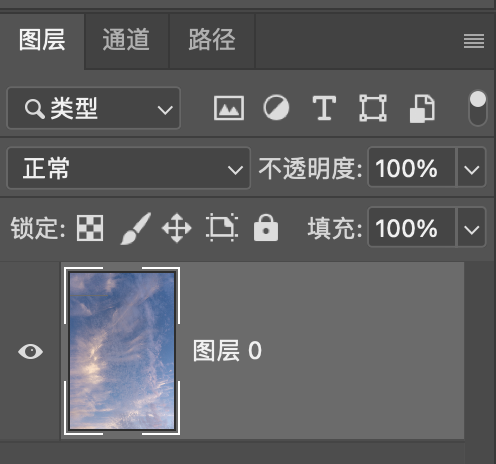
\includegraphics[width=0.4\linewidth]{figure/fillandopacity}
	\caption{"不透明度"和"填充"所在位置}
	\label{fig:fillandopacity}
\end{figure}

填充还有一个名字叫填充不透明度
% TODO: \usepackage{graphicx} required
\begin{figure}[!htb]
	\centering
	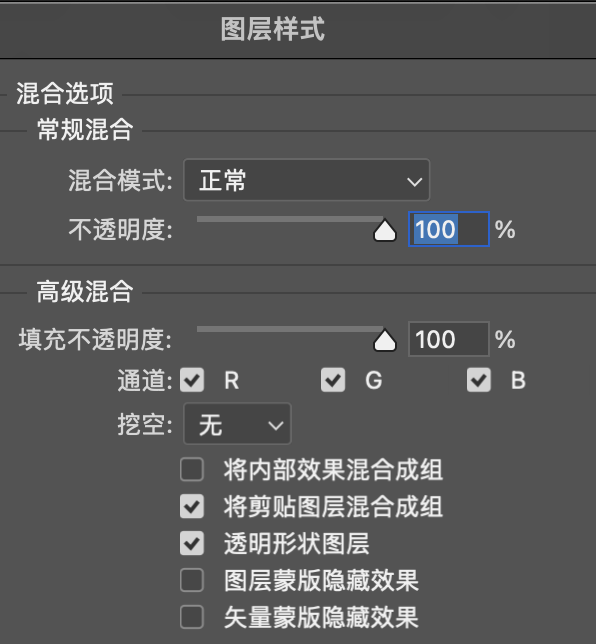
\includegraphics[width=0.4\linewidth]{figure/fill3}
	\caption{"填充"和"填充不透明度"}
	\label{fig:fill2}
\end{figure}

\section{ 不透明度和填充公式}
不透明度的英文单词是$Opacity$,填充的英文单词是$fill$,两者在图层混合模式中有时相同有时不同。具体我们会在后面说明。简单描述二者的区别,就是,不透明度就是将基础图层$B$和结果图层$R$,使用$Opacity$比例进行混合,公式如下:
\begin{equation}
	Opacity(b,a)= op\times b + (1-op)\times BlendMode(b,a)
\end{equation}

其中$op$代表不透明度
并且,填充的优先级高于不透明度,如果让两者一起产生效果则公式为:
\begin{equation}
	Opacity(b,a)= op\times b + (1-op)\times Fill(b,a)
\end{equation}
\begin{notice}
\item $Fill(b,a)= BlendMode(b,a\times fill)$这只是一个原则公式,具体情况要视具体模式确定,每一种计算方式都有细微区别。我们在此处不给出具体的公式和代码,但是我们在每一种中,我们会具体实现。
\end{notice}

\section{单纯混合模式与二者使用的区别}
填充的计算方式有八个和其他的不同,并且此时和不透明度的计算方法不一样。除了这八个,不透明度和填充变化的结果是相同的。

\penmark{他们分别是}

\begin{itemize}
	\item  线性加深
	\item  颜色加深
	\item  线性减淡
	\item  颜色减淡
	\item  线性光(线性减淡+线性加深)
	\item  亮光(颜色减淡+颜色加深)
	\item  实色混合(线性减淡+线性加深 或者 颜色减淡+颜色加深)
	\item  差值
\end{itemize}

如果使用一句话概括这二者的区别就是:
\begin{notice}
	\item 填充会让当前混合模式的效果弱化,弱化的程度取决于$fill$的大小。
	\item 不透明度决定了当前混合模式结果图层和基础图层混合的比例,opacity越大,结果图层占比越大。
	\item 结合前面的例子,填充越大放的茶叶就越多,不透明度越大,最后添加的水就越少。
\end{notice}
\section{ 代码实现}
\subsection{不透明度}
\begin{lstlisting}
	public static BlendColor Opacity(BlendColor colorBase, BlendColor colorResult, double opacity) {
		double redOpacity = colorResult.red.value *opacity + colorBase.red.value* (1 - opacity);
		double greenOpacity = colorResult.green.value *opacity + colorBase.green.value* (1 - opacity);
		double blueOpacity = colorResult.blue.value *opacity + colorBase.blue.value* (1 - opacity);
		return new BlendColor(redOpacity, greenOpacity, blueOpacity);
	}
\end{lstlisting}
\subsection{填充}
填充具体情况具体分析
\section{不透明度和填充与图层样式}
这里顺便提一下图层样式在两种调节方式下有什么区别,图层样式,比如描边,如果调节不透明度,则会同主体一起变,但是如果只调节填充,则只有主体会变而样式不会变。
\chapter{图层混合模式的种类}
\begin{introduction}
	\item  本章介绍按照不同方式对图层混合模式的分类
	\item  从不同的角度,图层混合模式有不同的种类
\end{introduction}
\section{ 色彩空间分类}
分类方法有很多,如果按照色彩空间,可以分成两类,RGB和HSY
\subsection{ RGB}
除颜色组
\subsection{ HSY}
颜色组
\section{ 是否产生新的数值}
如果根据运算方式,可以分成两类,一类是替换式,一类是融合式
\subsection{ 替换式}
\begin{itemize}
	\item  正常组(正常,溶解)
	\item 变暗组(变暗,深色)
	\item 变亮组(变亮,浅色)
	\item 颜色组(色相,饱和度,颜色,明度)
\end{itemize}
\begin{notice}
\item 这种式的特点是,不会产生新的东西,只会复用之前的东西,比如正常组,正常就是直接使用混合图层作为结果,变暗组的变暗是使用基础图层和混合图层中通道较小的值组成新的像素,深色则是比较基础图层和混合图层通道值的和取小的作为结果,颜色组,则是根据HSY色彩空间,直接替换 HSY的数值,并且再转换为RGB,本质也是没有新的东西产生。
\end{notice}

\subsection{ 融合式}
\begin{itemize}
	\item 变暗组(正片叠底,颜色加深,线性加深)
	\item 变亮组(滤色,颜色减淡,线性减淡)
	\item 对比度组(叠加,柔光,强光,亮光,线性光,点光,实色混合)
	\item 差值组(差值,排除,减去,划分)
\end{itemize}
\begin{notice}
	\item 
 虽然点光是变暗和变亮的混合,但是混合过程中做了处理,所以此处我们也按照融合式对待,此类的特点是,会产生新的数值。融合式就是产生了新的数值,比如正片叠底,结果图层的数值由基础图层和混合图层的乘积得到,他是不同于基础图层和混合图层的值。
 \end{notice}
\section{ 是否顺序相关}
\indent 如果根据是否受到图层顺序影响,如果
\begin{equation}
BlendMode(b,a)=BlendMode(a,b)
\end{equation}

则说明结果不受图层顺序影响,前提是不调节$fill$和$Opacity$
\subsection{ 顺序无关}
\begin{itemize}
	\item 变暗组 (变暗,线性加深,正片叠底,深色)
	\item 变亮组 (变亮,线性减淡,滤色,浅色)
	\item 对比度组 (实色混合)
	\item 差值组(差值,排除)
\end{itemize}

\subsection{ 顺序相关}
\begin{itemize}
	\item 正常组 (正常,溶解)
	\item 变暗组(颜色加深)
	\item 变亮组(颜色减淡)
	\item 对比度组(叠加,柔光,强光,亮光,线性光,点光)
	\item 差值组(减去,划分)
	\item 颜色组(色相,饱和度,颜色,明度)
\end{itemize}
\section{ 是否fill和Opacity不同}

 也就是说,调节填充的百分比,和不透明度的百分比,即使数值相同,结果也有可能不同。
\subsection{ fill和Opacity产生不同影响}
\begin{itemize}
	\item 变暗组(线性加深,颜色加深)
	\item 变亮组(线性减淡,颜色减淡)
	\item 对比度组(亮光,线性光,实色混合)
	\item 差值组(差值)
\end{itemize}
\subsection{ fill和Opacity产生相同影响}
\begin{itemize}
	\item 正常组 (正常,溶解)
	\item 变暗组(变暗,正片叠底,深色)
	\item 变亮组(变亮,滤色,浅色)
	\item 对比度组(叠加,柔光,强光,点光)
	\item 差值组(排除,减去,划分)
	\item 颜色组(色相,饱和度,颜色,明度)
\end{itemize}
\begin{notice}
	\item 这里也不是说两者可以简单相乘,比如$fill=50\%$,$opacity=50\%$,的情况得到的结果,并不等于$fill=25\%$或者,$opacity=25\%$所得到的结果。其实理论应该是。
 \item	\begin{equation}
		\begin{aligned}
			r&=(BlendMode(b,a\times fill))\times op+b\times op\\&=(fill\times a+(1-fill)\times b)\times op+b\times op
		\end{aligned}
	\end{equation}
\end{notice}

\chapter{普通组}

\begin{introduction}
	\item 普通组包括正常模式和溶解模式,他们的本质都是替换
	\item 虽然名为普通,但是几乎包含了我们需要掌握的所有内容
\end{introduction}
\section{ 正常Normal}
正常模式是一切的基础,也是我们理解和掌握混合模式的基础,
正常模式可以看作是基于RGB颜色空间,也可以看作是基于HSY色彩空间

\subsection{ 公式(泡茶的方式,比如搅拌、静置)}

对于像素维度公式
\begin{equation}
	Pix_r=Normal(Pix_b,Pix_a)=Pix_a
\end{equation}

正常模式通道维度初始公式

\begin{equation}r=Normal(b,a)=a\end{equation}

\subsection{ 融合填充(放多少茶叶)}


\begin{equation}r=Fill(b,a)= fill\times a + (1-fill)\times b\end{equation}

\subsection{ 融合不透明度(太苦了,最后加点水)}

\begin{equation}r=Opacity(b,a)= op\times Fill(b,a) + (1-fill)\times b\end{equation}

对于整个像素

\begin{equation}(r_{rc},r_{gc},r_{bc})=Normal((b_{rc},b_{gc},b_{bc}),(a_{rc},a_{gc},a_{bc}))=(r_{rc},r_{gc},r_{bc})\end{equation}

后面的混合模式我们不再讨论整个像素的公式,我们只讨论某个通道的结果。

\subsection{ 整个像素融合填充}

这里不同的混合模式公式不一定相同。

\begin{equation}
	\begin{aligned}
		(r_{rc},r_{gc},r_{bc})=&Fill((b_{rc},b_{gc},b_{bc}),(a_{rc},a_{gc},a_{bc}))\\
		=&((fill\times a_{rc} + (1-fill)\times b_{rc}),\\&(fill\times a_{gc} + (1-fill)\times b_{gc}),\\&(fill\times a_{bc} + (1-fill)\times b_{bc}))
		\end{aligned}
\end{equation}

\subsection{ 整个像素融合不透明度}


\begin{equation}
	\begin{aligned}
		(r_{rc},r_{gc},r_{bc})=& Opacity((b_{rc},b_{gc},b_{bc}),(a_{rc},a_{gc},a_{bc}))\\=&((op\times Fill(a_{rc},b_{rc}) + (1-op)\times b_{rc}),\\&(op\times Fill(a_{gc},b_{gc} + (1-op)\times b_{gc}),\\&\textbf{}(op\times Fill(a_{bc},b_{bc} + (1-op)\times b_{bc}))
\end{aligned}
\end{equation}



\subsection{ 程序模拟该模式计算结果}
\begin{lstlisting}
	// 正常模式
	public static BlendColor Normal(BlendColor colorBase, BlendColor colorBlend, double fill, double opacity) {
		double red = colorBlend.red.get01Value() *fill + colorBase.red.get01Value()* (1 - fill);
		double green = colorBlend.green.get01Value() *fill + colorBase.green.get01Value()* (1 - fill);
		double blue = colorBlend.blue.get01Value() *fill + colorBase.blue.get01Value()* (1 - fill);
		return ColorUtils.Opacity(colorBase, new BlendColor(red *255, green* 255, blue * 255), opacity);
}
\end{lstlisting}

借助正常模式,我们可以看到不透明度和填充的关系,后面的模式讨论我们都不再说明像素级别的公式,因为没有必要,我们只讨论通道级别的公式。我们设定$fill$为$40\%$,$Opacity$ 为$60\%$
\begin{notice}
	\item 基础图层                RGB[111.00,  80.00,  60.00]~ HSY[23.53,  51.00,  87.10 ]~ HSB[ 23.53,  45.95,  43.53]
	
	\item 混合图层                RGB[ 80.00,  70.00, 156.00]~ HSY[246.98,  86.00,  82.46]~ HSB[246.98,  55.13,  61.18]
\end{notice}

我们在PS中使用这两种颜色进行验证,发现符合我们的算法。
\begin{result}
	\item 正    常(Normal)        RGB[103.56,  77.60,  83.04]~ HSY[347.43,  25.96,  85.99]~ HSB[347.43,  25.07,  40.61]
\end{result}
\newpage
\subsection{ 验证}
% TODO: \usepackage{graphicx} required
\begin{figure}[h!]
	\centering
	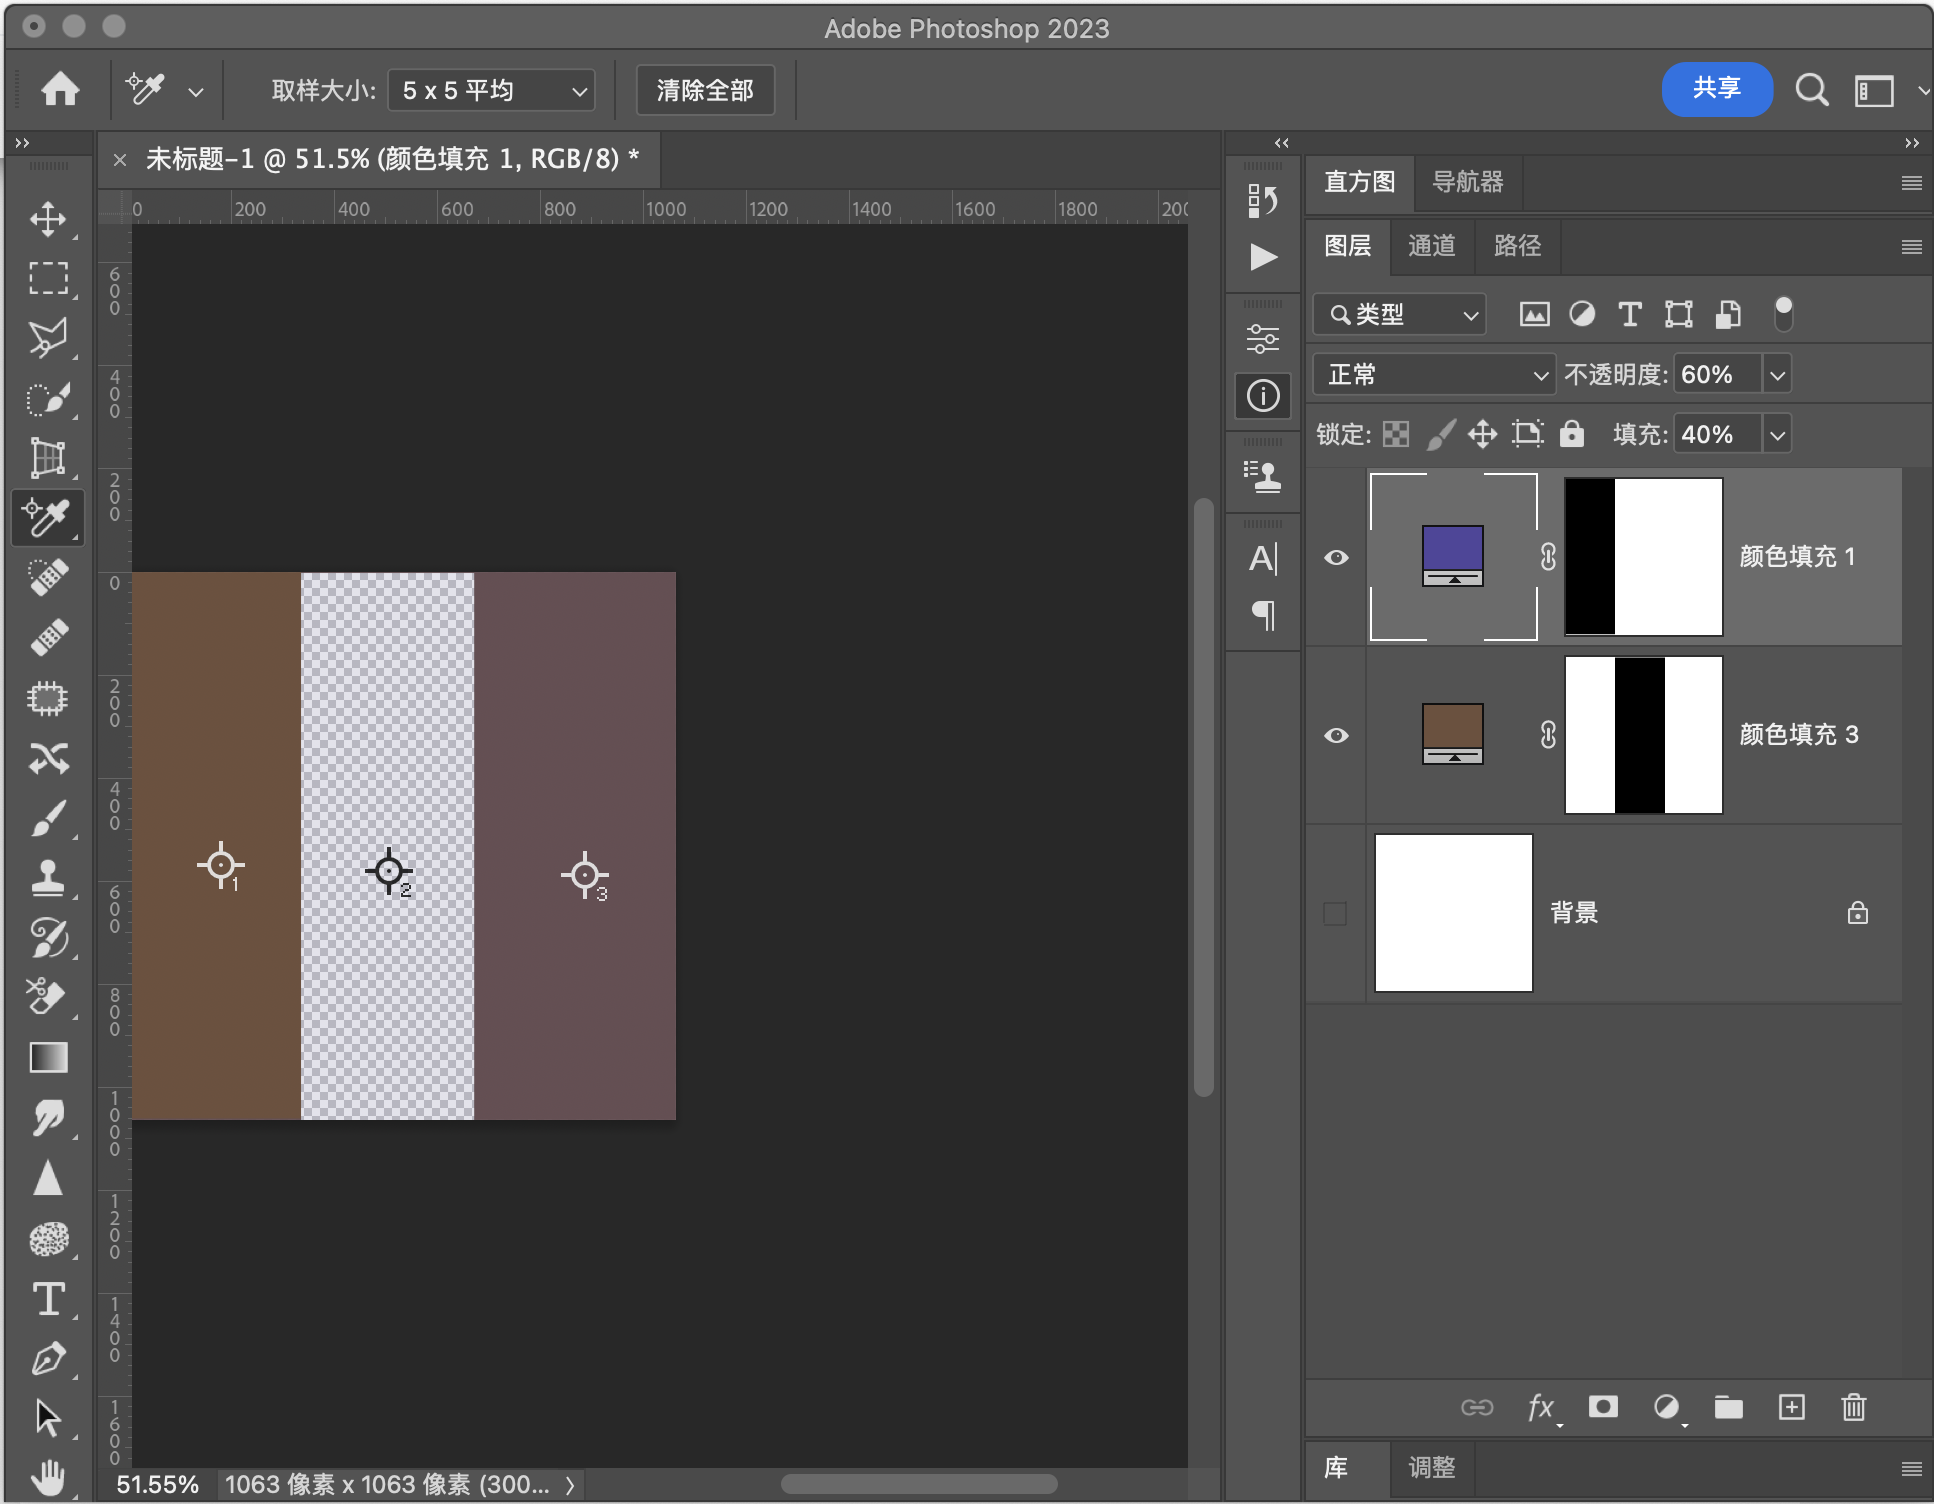
\includegraphics[width=\linewidth]{figure/normal}
	\caption{}
	\label{fig:normal}
\end{figure}
%\subsection{ 用途示例}
%该模式是默认模式,在不调节填充和不透明度的情况下,就是上方像素点覆盖下方的像素点。
%结合不透明度或者填充,可以实现和下方图层的简单混色。
\newpage
\section{ 溶解Dissolve}
溶解模式是正常组的第二种模式,他依靠替换,并且其对不透明度是免疫的。
\subsection{ 溶解模式初始公式}
\begin{equation}r=Dissolve(b,a)=a\end{equation}
\subsection{ 如果融合了填充}
\begin{equation}r=Fill(b,a)= Random_{fill}(Dissolve(b,a),b)\end{equation}
\begin{notice}
\item 不透明度对溶解模式是无效的。
\item $fill$的值越大,则下层像素暴露的可能性越小。
\end{notice}


\subsection{ 程序模拟该模式计算结果}

\begin{lstlisting}	// 溶解模式
	public static BlendColor Dissovle(BlendColor colorBase, BlendColor colorBlend, double fill, double opacity) {
		double rand = Math.random(); // 产生随机数
		if (rand < fill) {
			return colorBlend;
		} else {
			return colorBase;
		}
	}
\end{lstlisting}
\begin{result}
\item 	溶    解(Dissolve)      RGB[111.00,  80.00,  60.00]~ HSY[23.53,  51.00,  87.10 ]~ HSB[ 23.53,  45.95,  43.53]
\end{result}

\newpage
\subsection{ 验证}
\begin{notice}
	\item 溶解模式是根据概率来实现决定显示下方像素还是上方像素,于是取样点不同,则结果可以是上方的像素也可以是下方的像素。
	\end{notice}
\begin{figure}[!h]
	\centering
	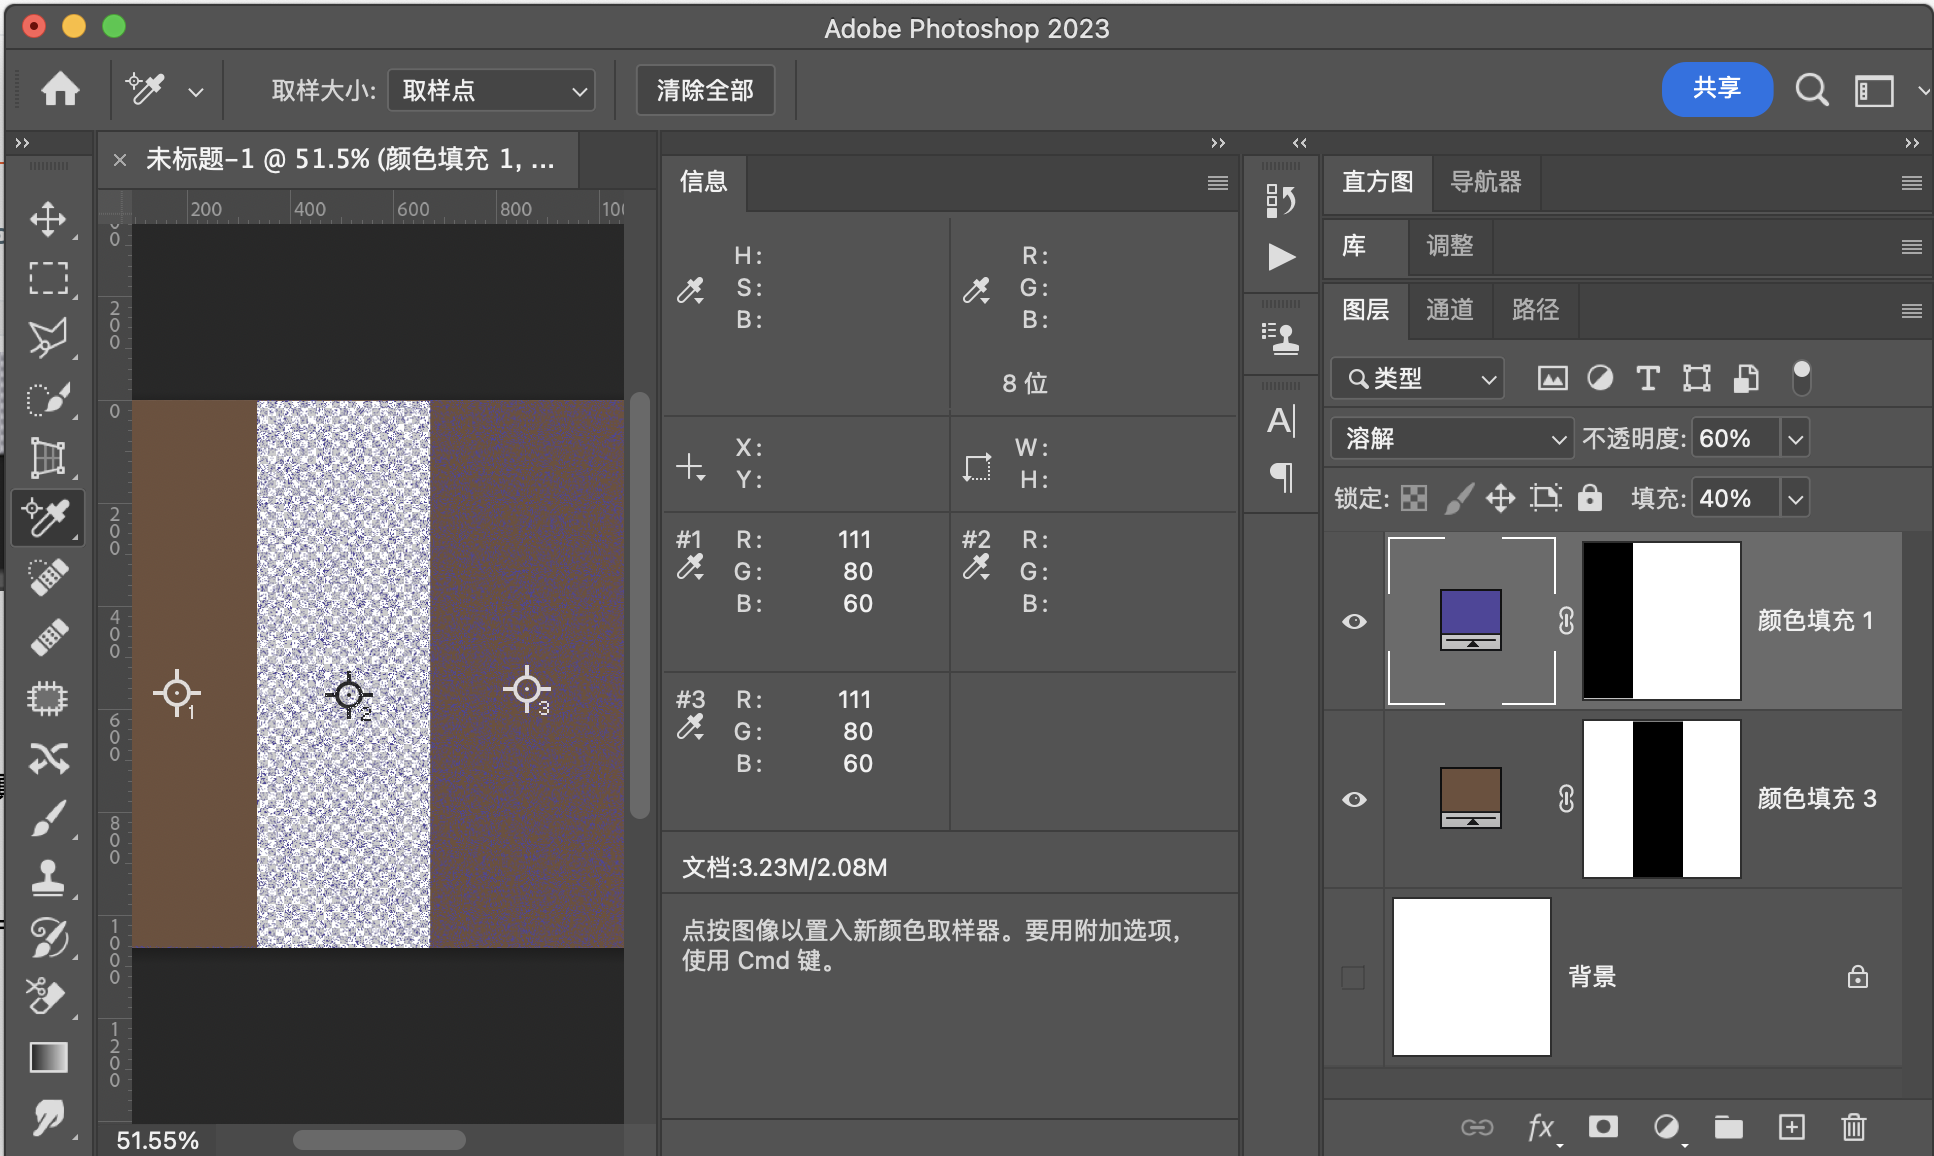
\includegraphics[width=\textwidth]{dissolve.png}
\end{figure}

\subsection{ 用途示例}

可以通过该模式实现一下粒子效果

\chapter{变暗组}
\begin{introduction}
	\item 这一组是基于RGB色彩空间,RGB三个通道的数值取值范围是$[0,255]$,归一化之后取值范围是$[0,1]$。这一组就是利用一系列运算让基础图层的三个通道的数值或者他们的和小于等于原值。这也是变暗组的本质。
	和下面的变亮组一样,变暗组有两种方式将通道值或者通道值的和变小,那就是替换和运算,替换包括变暗和深色,运算包括其他三种。
\end{introduction}


\section{ 变暗模式Darken}

如果将基础图层每个像素每个通道的数值都变小,最简单的方式就是选择原图图层像素通道值和混合图层像素通道值中比较小的那个作为结果图层像素通道值,这样的图层中每个像素点的通道值都小于等于原值,图像自然就会变暗。

\subsection{ 公式}


\begin{equation}r=Darken(b,a)=Min(b,a)\end{equation}

\subsection{ 融合填充}
\begin{equation}r= Fill(b,a) =fill\times Min(b,a)+(1-fill)\times b\end{equation}
\subsection{ 融合不透明度}
\begin{equation}r=Opacity(b,a)=op\times Fill(b,a)+(1-op)\times b\end{equation}
\subsection{ 映射面和同图等效曲线}
同图曲线表达式
\begin{equation}
	r=Darken(b,b)=b
	\end{equation}
\begin{notice}
	\item 这里我们简单认为fill和opacity都是100,因为我们日常使用中几乎用不到改变这两个值并且需要模拟同图曲线的情况,使用这里只讨论最简单的类型。但是其他类型可以通过我们提供的公式自行推导,但是这里没有必要写出来。下同。
\end{notice}
\begin{figure}[!htb]
	\centering
	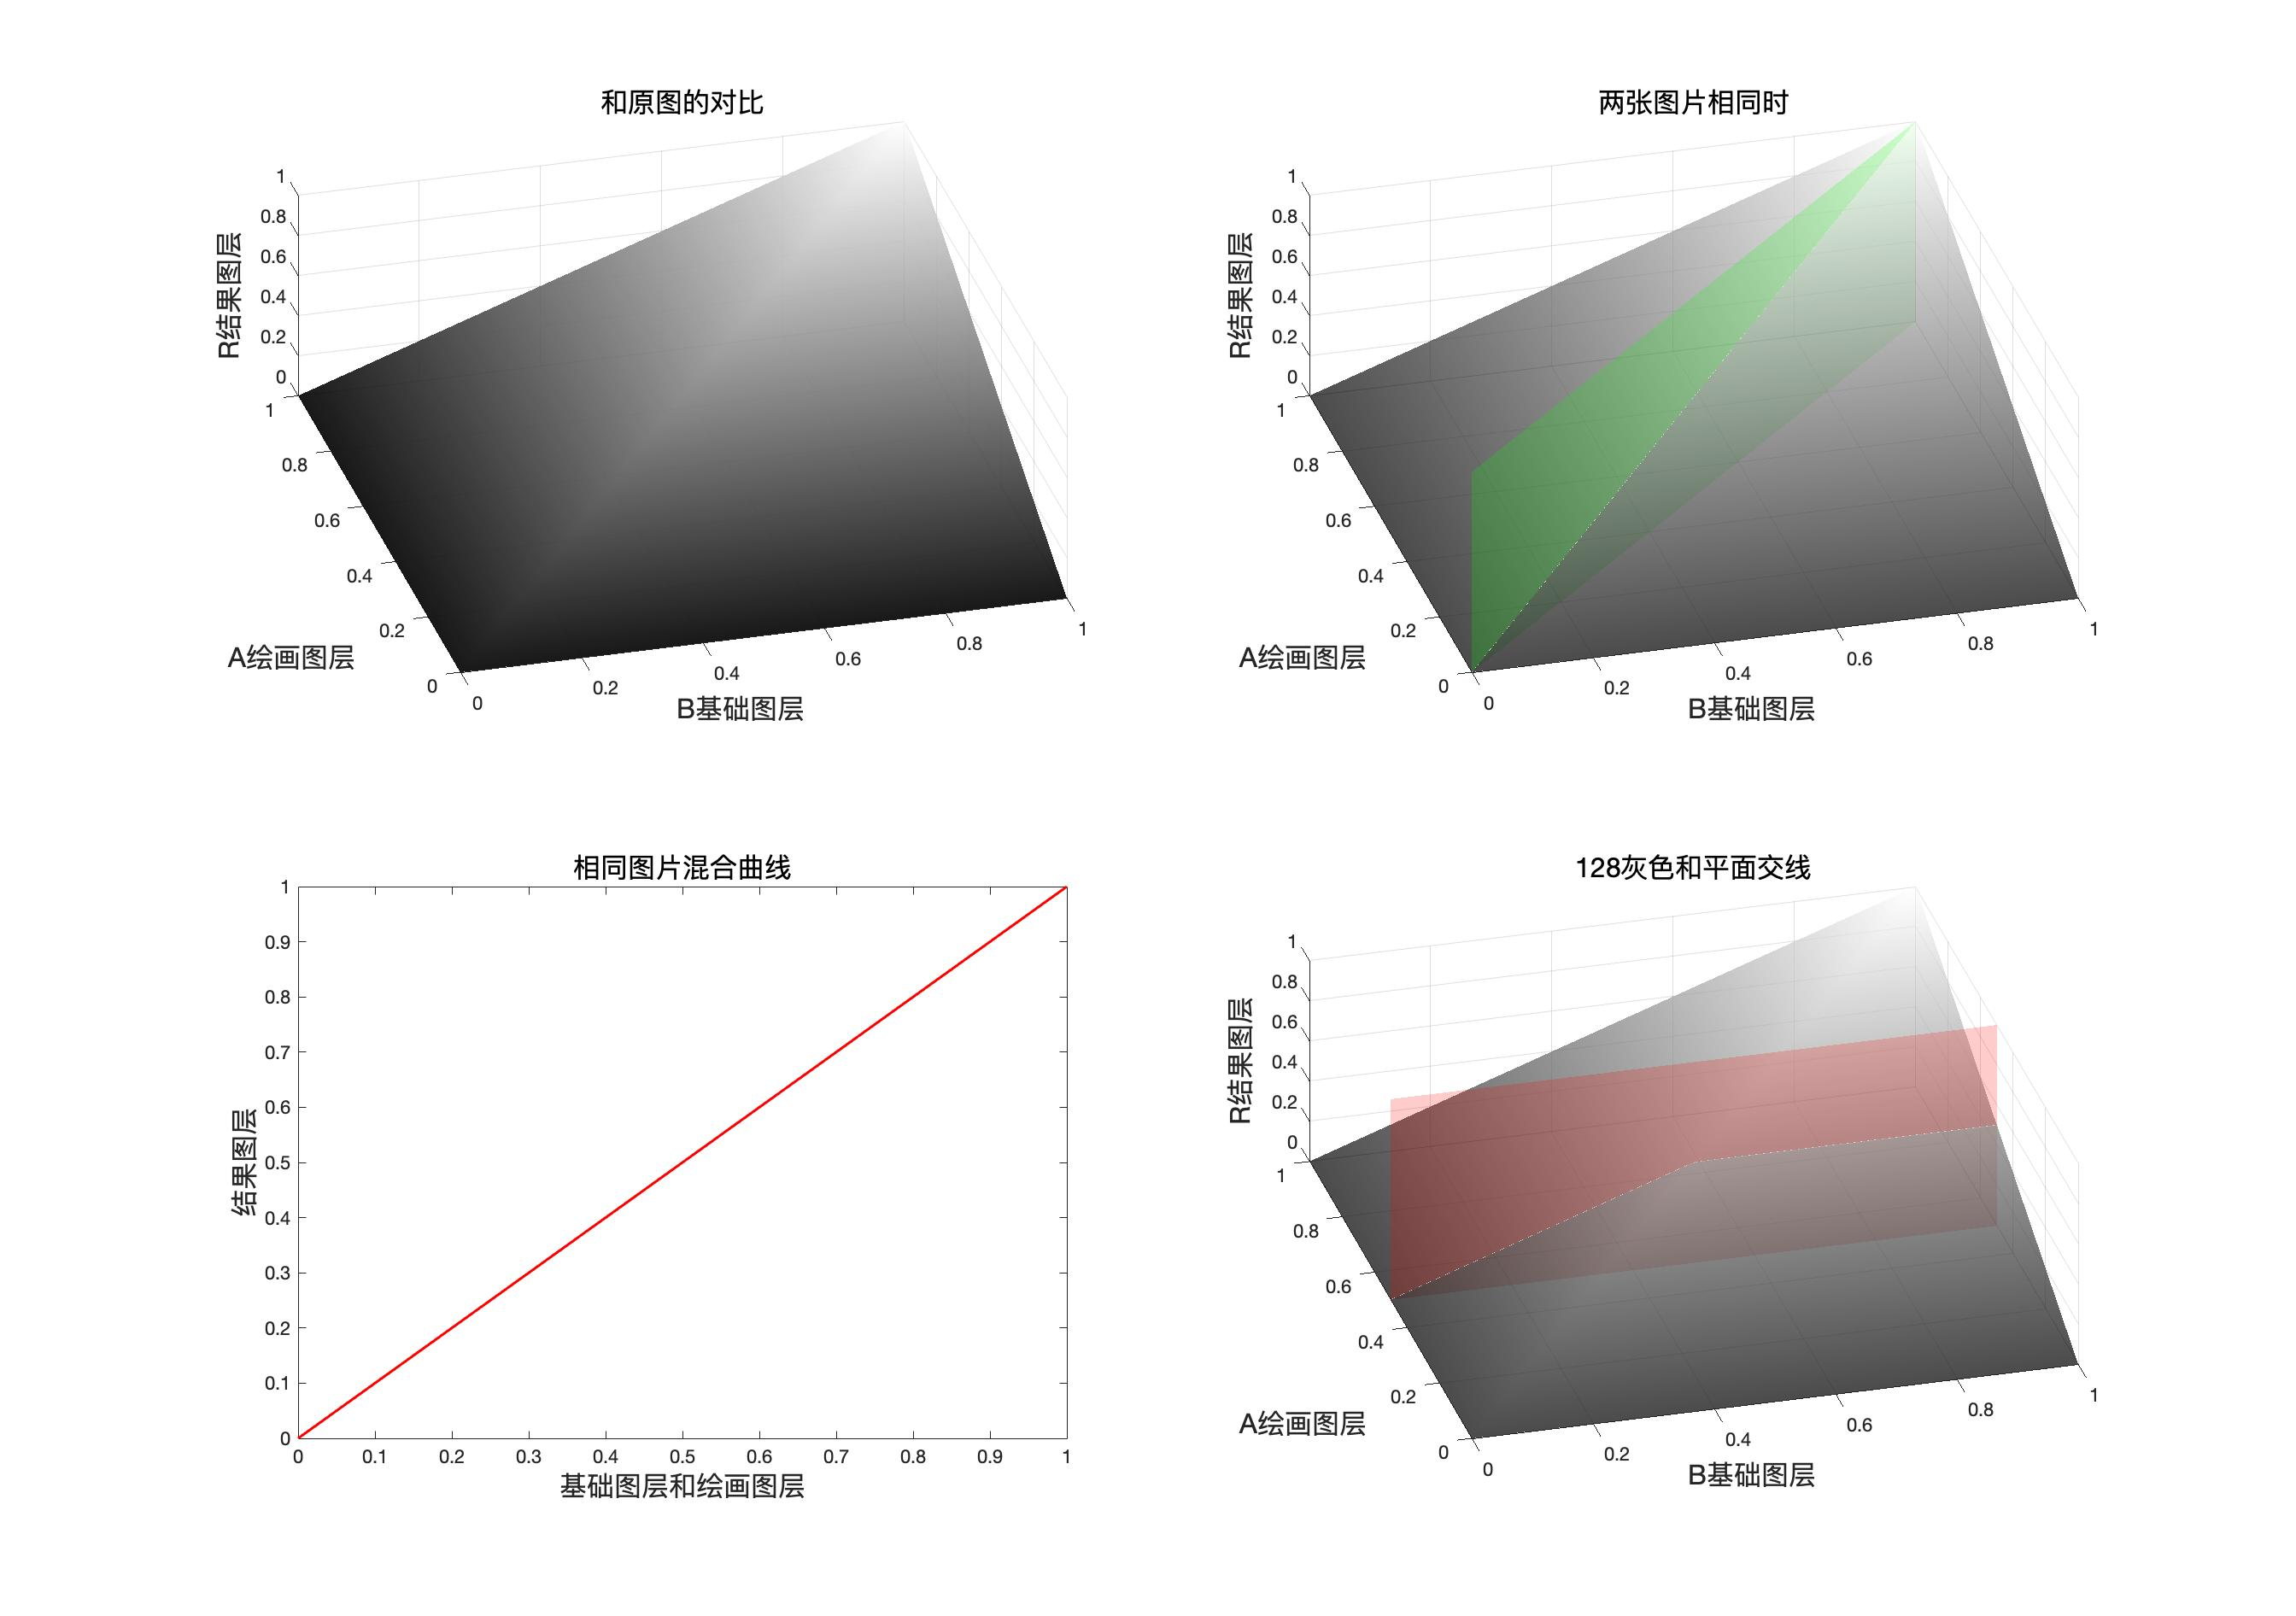
\includegraphics[width=1.1\linewidth]{figure/变暗模式.jpg}
	\caption{}
	\label{fig:}
\end{figure}
\newpage
\subsection{ 程序模拟该模式计算结果}
\begin{lstlisting}
	// 变暗
	public static BlendColor Darken(BlendColor colorBase, BlendColor colorBlend, double fill, double opacity) {
		double red = DarkenChannel(colorBase.red.get01Value(), colorBlend.red.get01Value(), fill);
		double green = DarkenChannel(colorBase.green.get01Value(), colorBlend.green.get01Value(), fill);
		double blue = DarkenChannel(colorBase.blue.get01Value(), colorBlend.blue.get01Value(), fill);
		return ColorUtils.Opacity(colorBase, new BlendColor(red *255, green* 255, blue * 255), opacity);
	}
	
	private static double DarkenChannel(double base, double blend, double fill) {
		return Math.min(base, blend) * fill + (1 - fill) * base;
	}
\end{lstlisting}


\begin{result}
	\item 变    暗(Darken)        RGB[103.56,  77.60,  60.00]~ HSY[24.24,  43.56,  83.45 ]~ HSB[ 24.24,  42.06,  40.61]
\end{result}
\subsection{ 验证}
% TODO: \usepackage{graphicx} required
\begin{figure}[!htb]
	\centering
	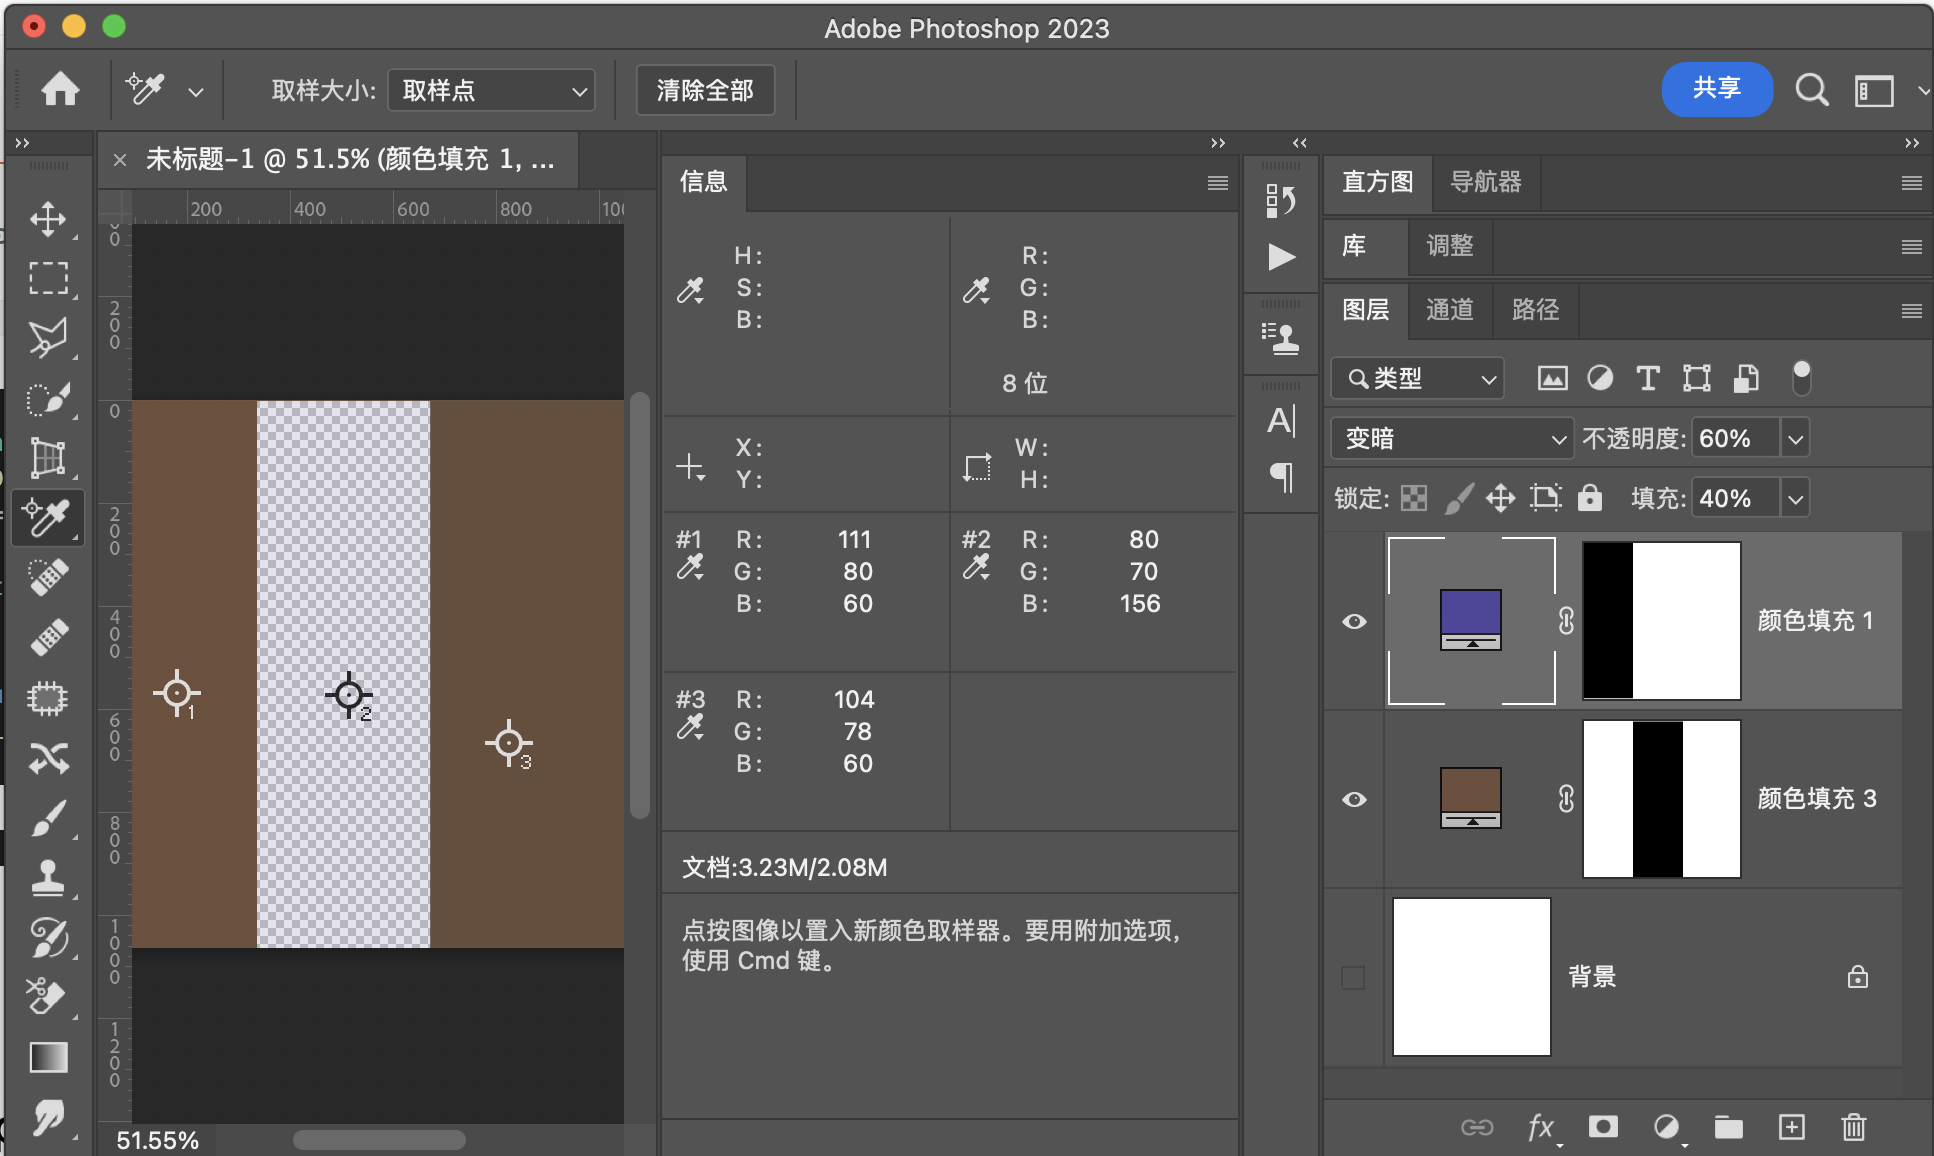
\includegraphics[width=\linewidth]{figure/darken}
	\caption{}
	\label{fig:darken}
\end{figure}

%
%\subsection{ 用途示例}
%
%1:组合成为对比度组的点光Pinlight模式
%
%2:此处是深色模式的简化版本,但是我们还是可以通过它来实现一些溶图操作

\newpage
\section{ 正片叠底Multiply}

如果将混合图层像素的通道数值和原图像素通道数值相乘,则因为归一化之后的数值都是小于等于1的所以,原值乘一个小于1的数值一定小于等于原来的值。所以图像会变暗。

\subsection{ 公式}


\begin{equation}r=Multiply(b,a)=b\times a\end{equation}

\subsection{ 融合填充}


\begin{equation}r= Fill(b,a) =fill\times b\times a+(1-fill)\times b\end{equation}

\subsection{ 融合不透明度}


\begin{equation}r=Opacity(b,a)=op\times Fill(b,a)+(1-op)\times b\end{equation}

\subsection{ 映射面和同图等效曲线}

正片叠底的映射面,同图面,同图曲线和中性灰平面
% TODO: \usepackage{graphicx} required
\begin{figure}[!htb]
	\centering
	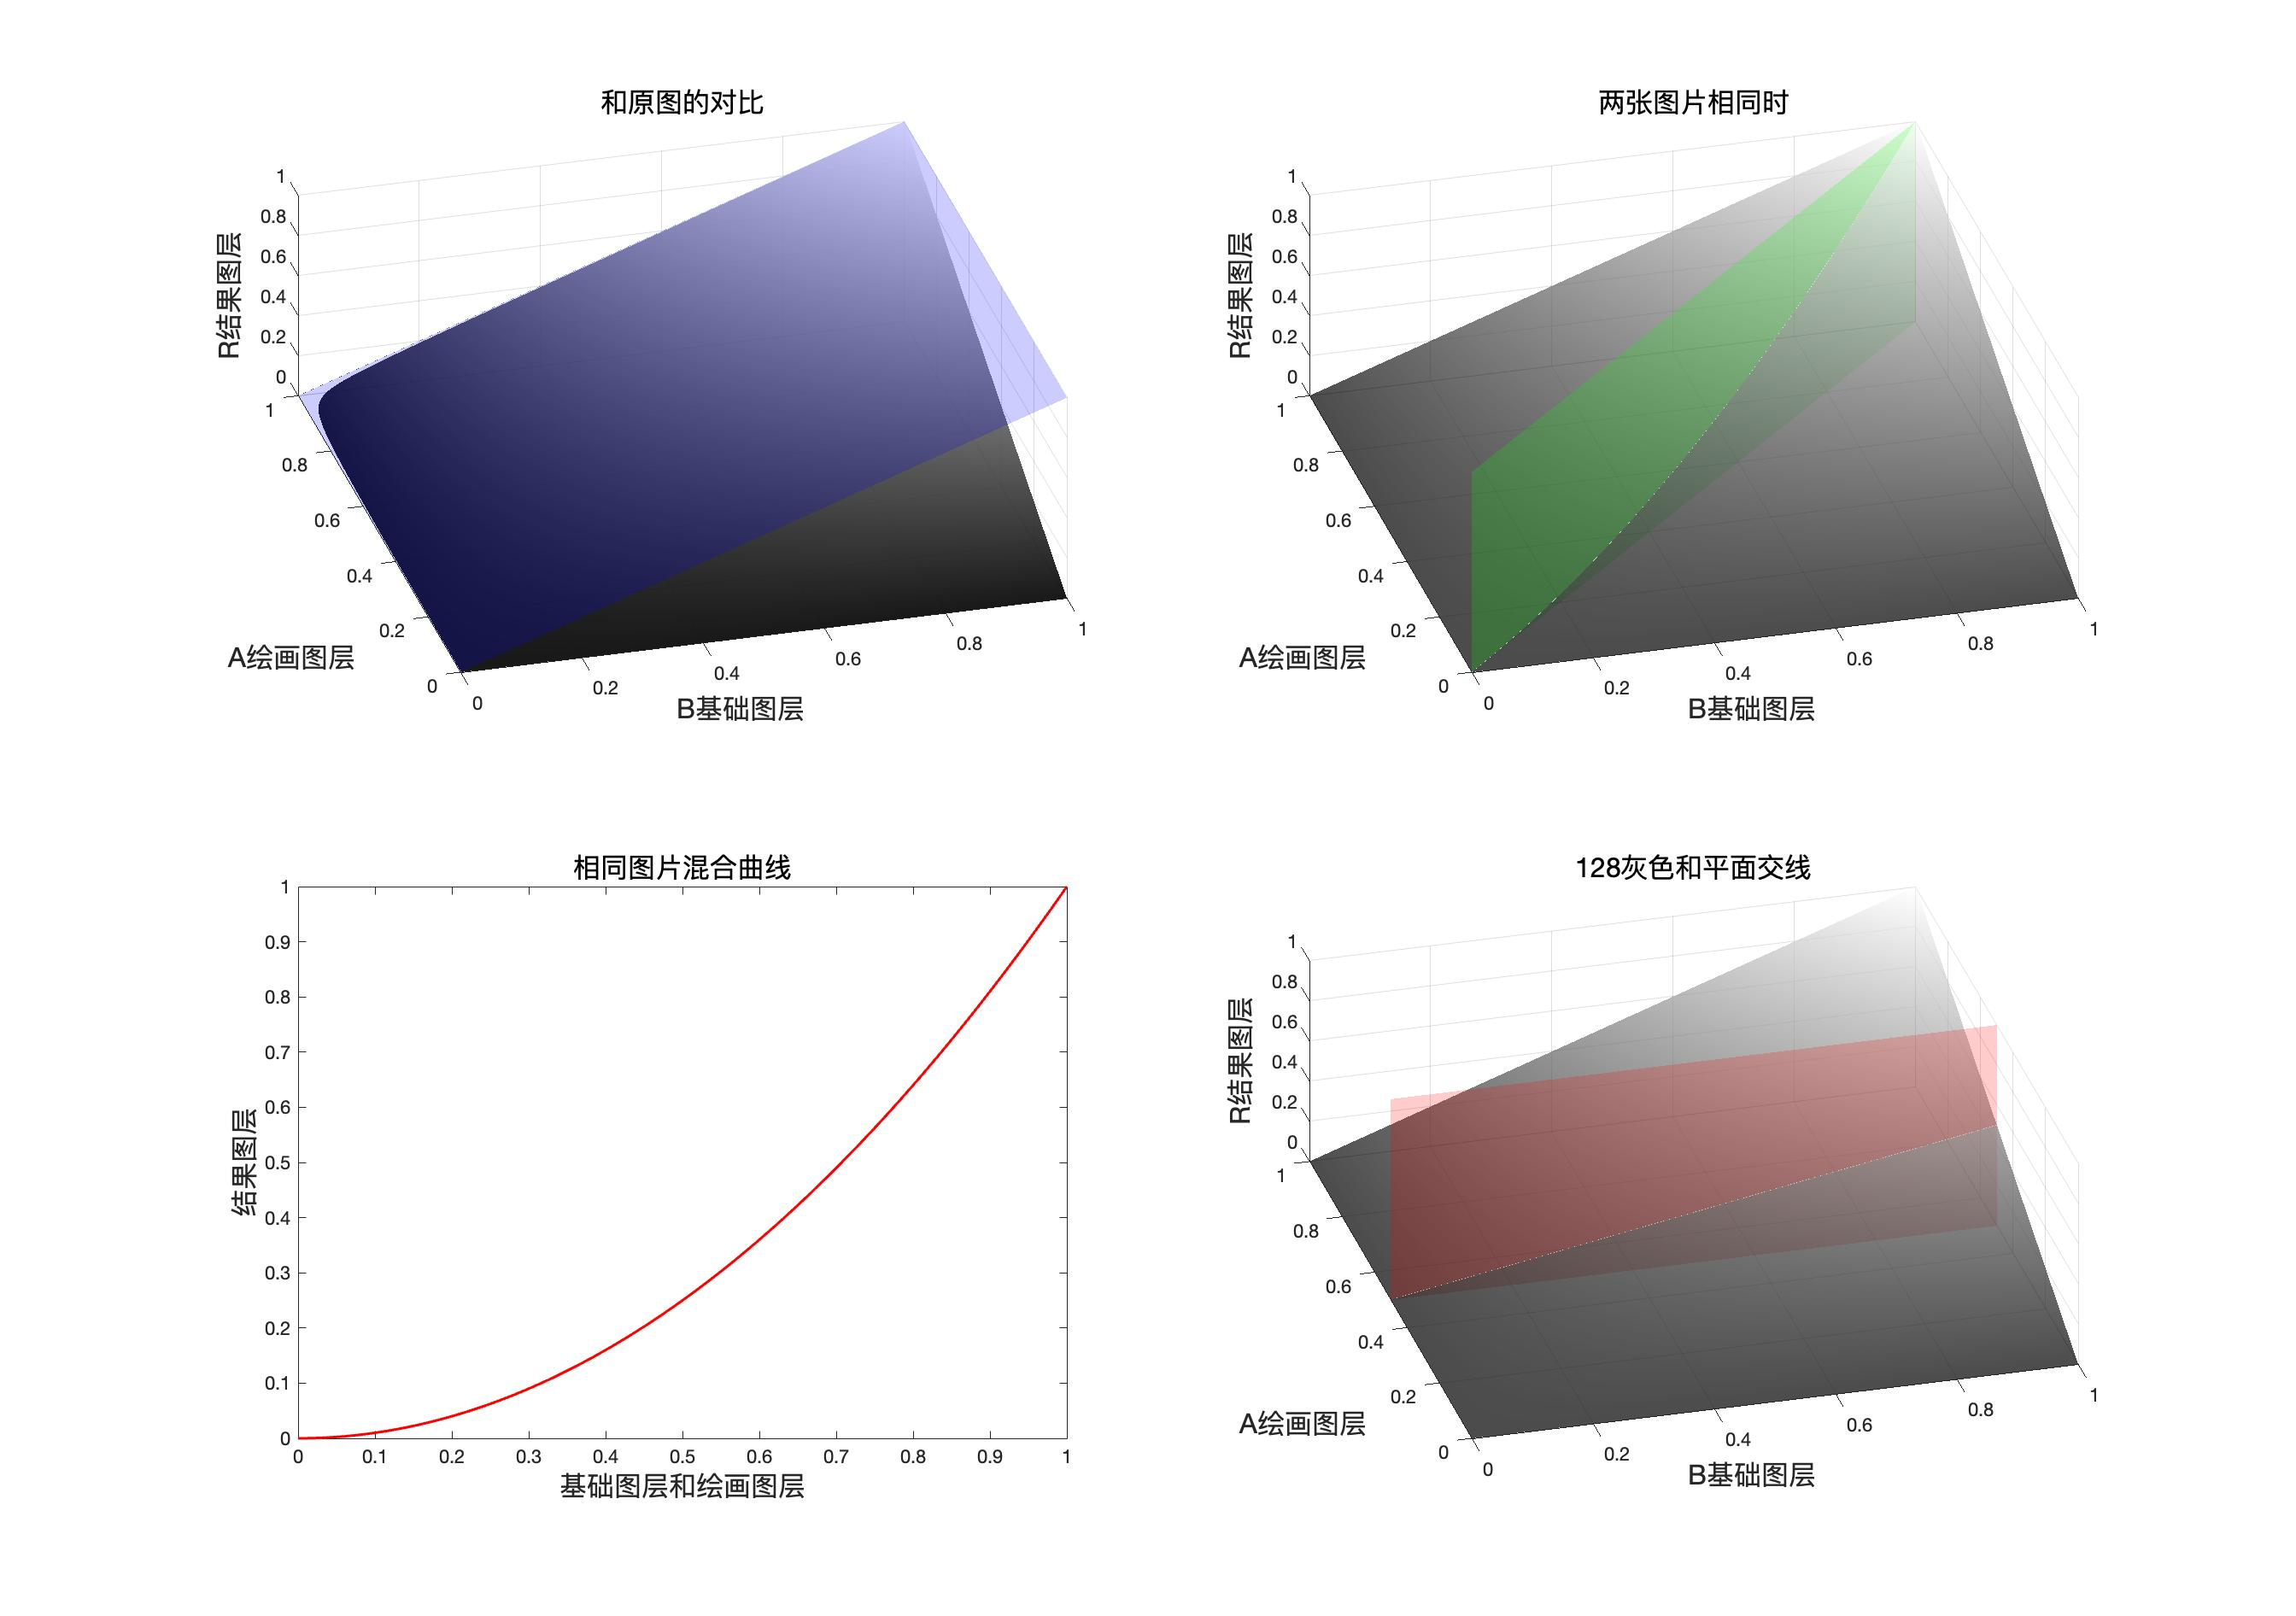
\includegraphics[width=\linewidth]{figure/正片叠底.jpg}
	\caption{}
	\label{fig:}
\end{figure}


\subsection{ 同图曲线表达式}


\begin{equation}r=Multiply(b,b)= b^2\end{equation}

\subsection{ 程序模拟该模式计算结果}

\begin{lstlisting}
	// 正片叠底
	public static BlendColor Mulitply(BlendColor colorBase, BlendColor colorBlend, double fill, double opacity) {
		double red = MulitplyChannel(colorBase.red.get01Value(), colorBlend.red.get01Value(), fill);
		double green = MulitplyChannel(colorBase.green.get01Value(), colorBlend.green.get01Value(), fill);
		double blue = MulitplyChannel(colorBase.blue.get01Value(), colorBlend.blue.get01Value(), fill);
		return ColorUtils.Opacity(colorBase, new BlendColor(red * 255, green * 255, blue * 255), opacity);
	}
	
	private static double MulitplyChannel(double base, double blend, double fill) {
		return ColorUtils.round((base * blend) * fill + (1 - fill) * (base), 1, 0);
	}
\end{lstlisting}



\begin{result}
\item 正片叠底(Mulitply)      RGB[ 92.72,  66.07,  54.41]~ HSY[18.26,  38.31,  72.78 ]~ HSB[ 18.26,  41.32,  36.36]
\end{result}

\subsection{ 验证}

\begin{figure}[!htb]
	\centering
	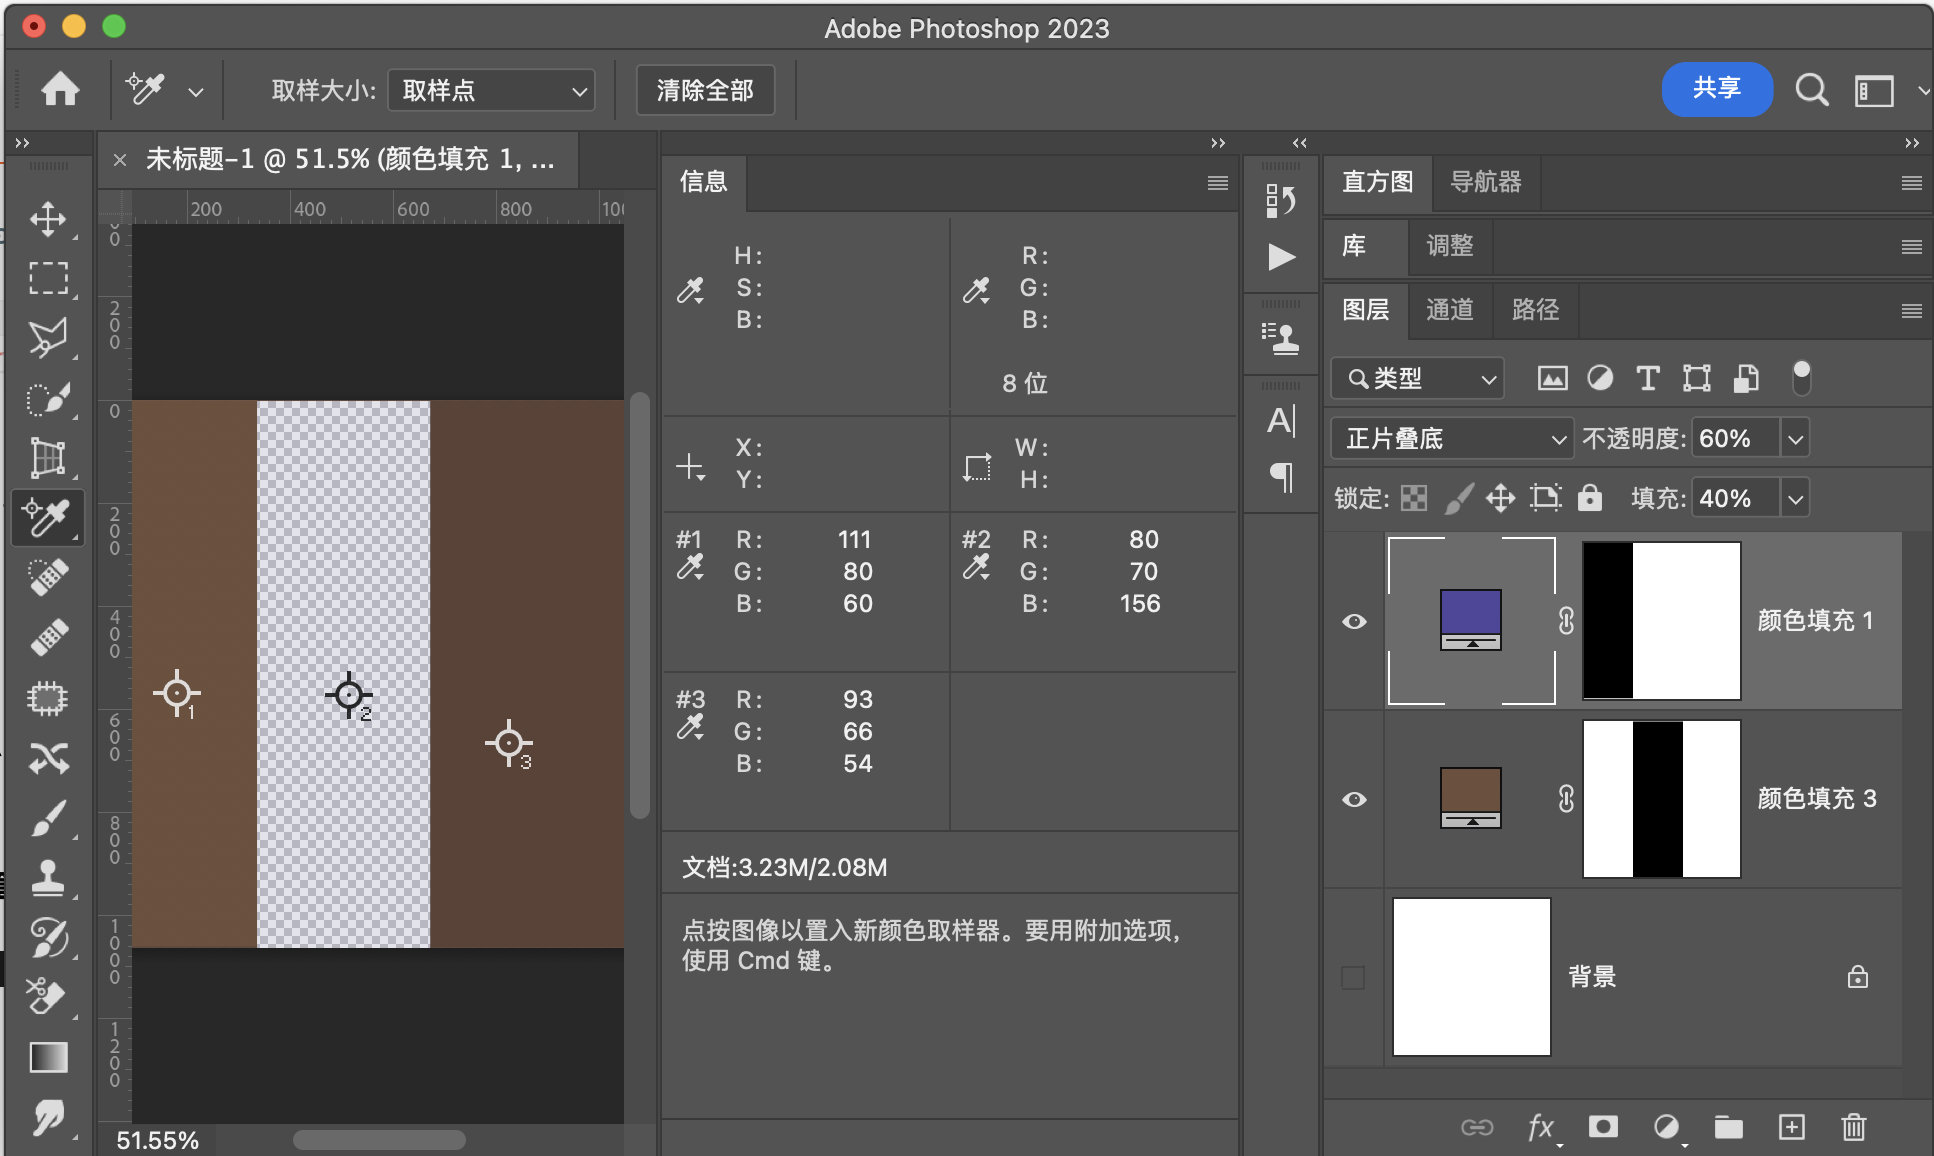
\includegraphics[width=\linewidth]{mulitply.png}
		\caption{正片叠底验证}
	\label{fig:}
\end{figure}
%\subsection{ 用途示例}
%
%1:和滤色模式组合成强光和叠加模式
%
%2:给比较亮的图片添加纹理
%
%3:扣除白色背景
\newpage
\section{ 线性加深LinearBurn}

此模式本质是减法,就是使用混合图层像素通道数值的补也就是附片和原图相减,如果大于1则取1小于0则取0,并且此模式需要对填充特殊处理。线性加深可以通过划分和颜色加深转化。

\subsection{ 公式}


\begin{equation}r=LinearBurn(b,a)=b-(1-a)=b+a-1\end{equation}

\subsection{ 融合填充}


\begin{equation}r= Fill(b,a) =b-(1-a)\times fill\end{equation}

\subsection{ 融合不透明度}


\begin{equation}r=Opacity(b,a)=op\times Fill(b,a)+(1-op)\times b\end{equation}

\subsection{ 映射面和同图等效曲线}

线性加深的映射面,同图面,同图曲线和中性灰平面
% TODO: \usepackage{graphicx} required
\begin{figure}[!htb]
	\centering
	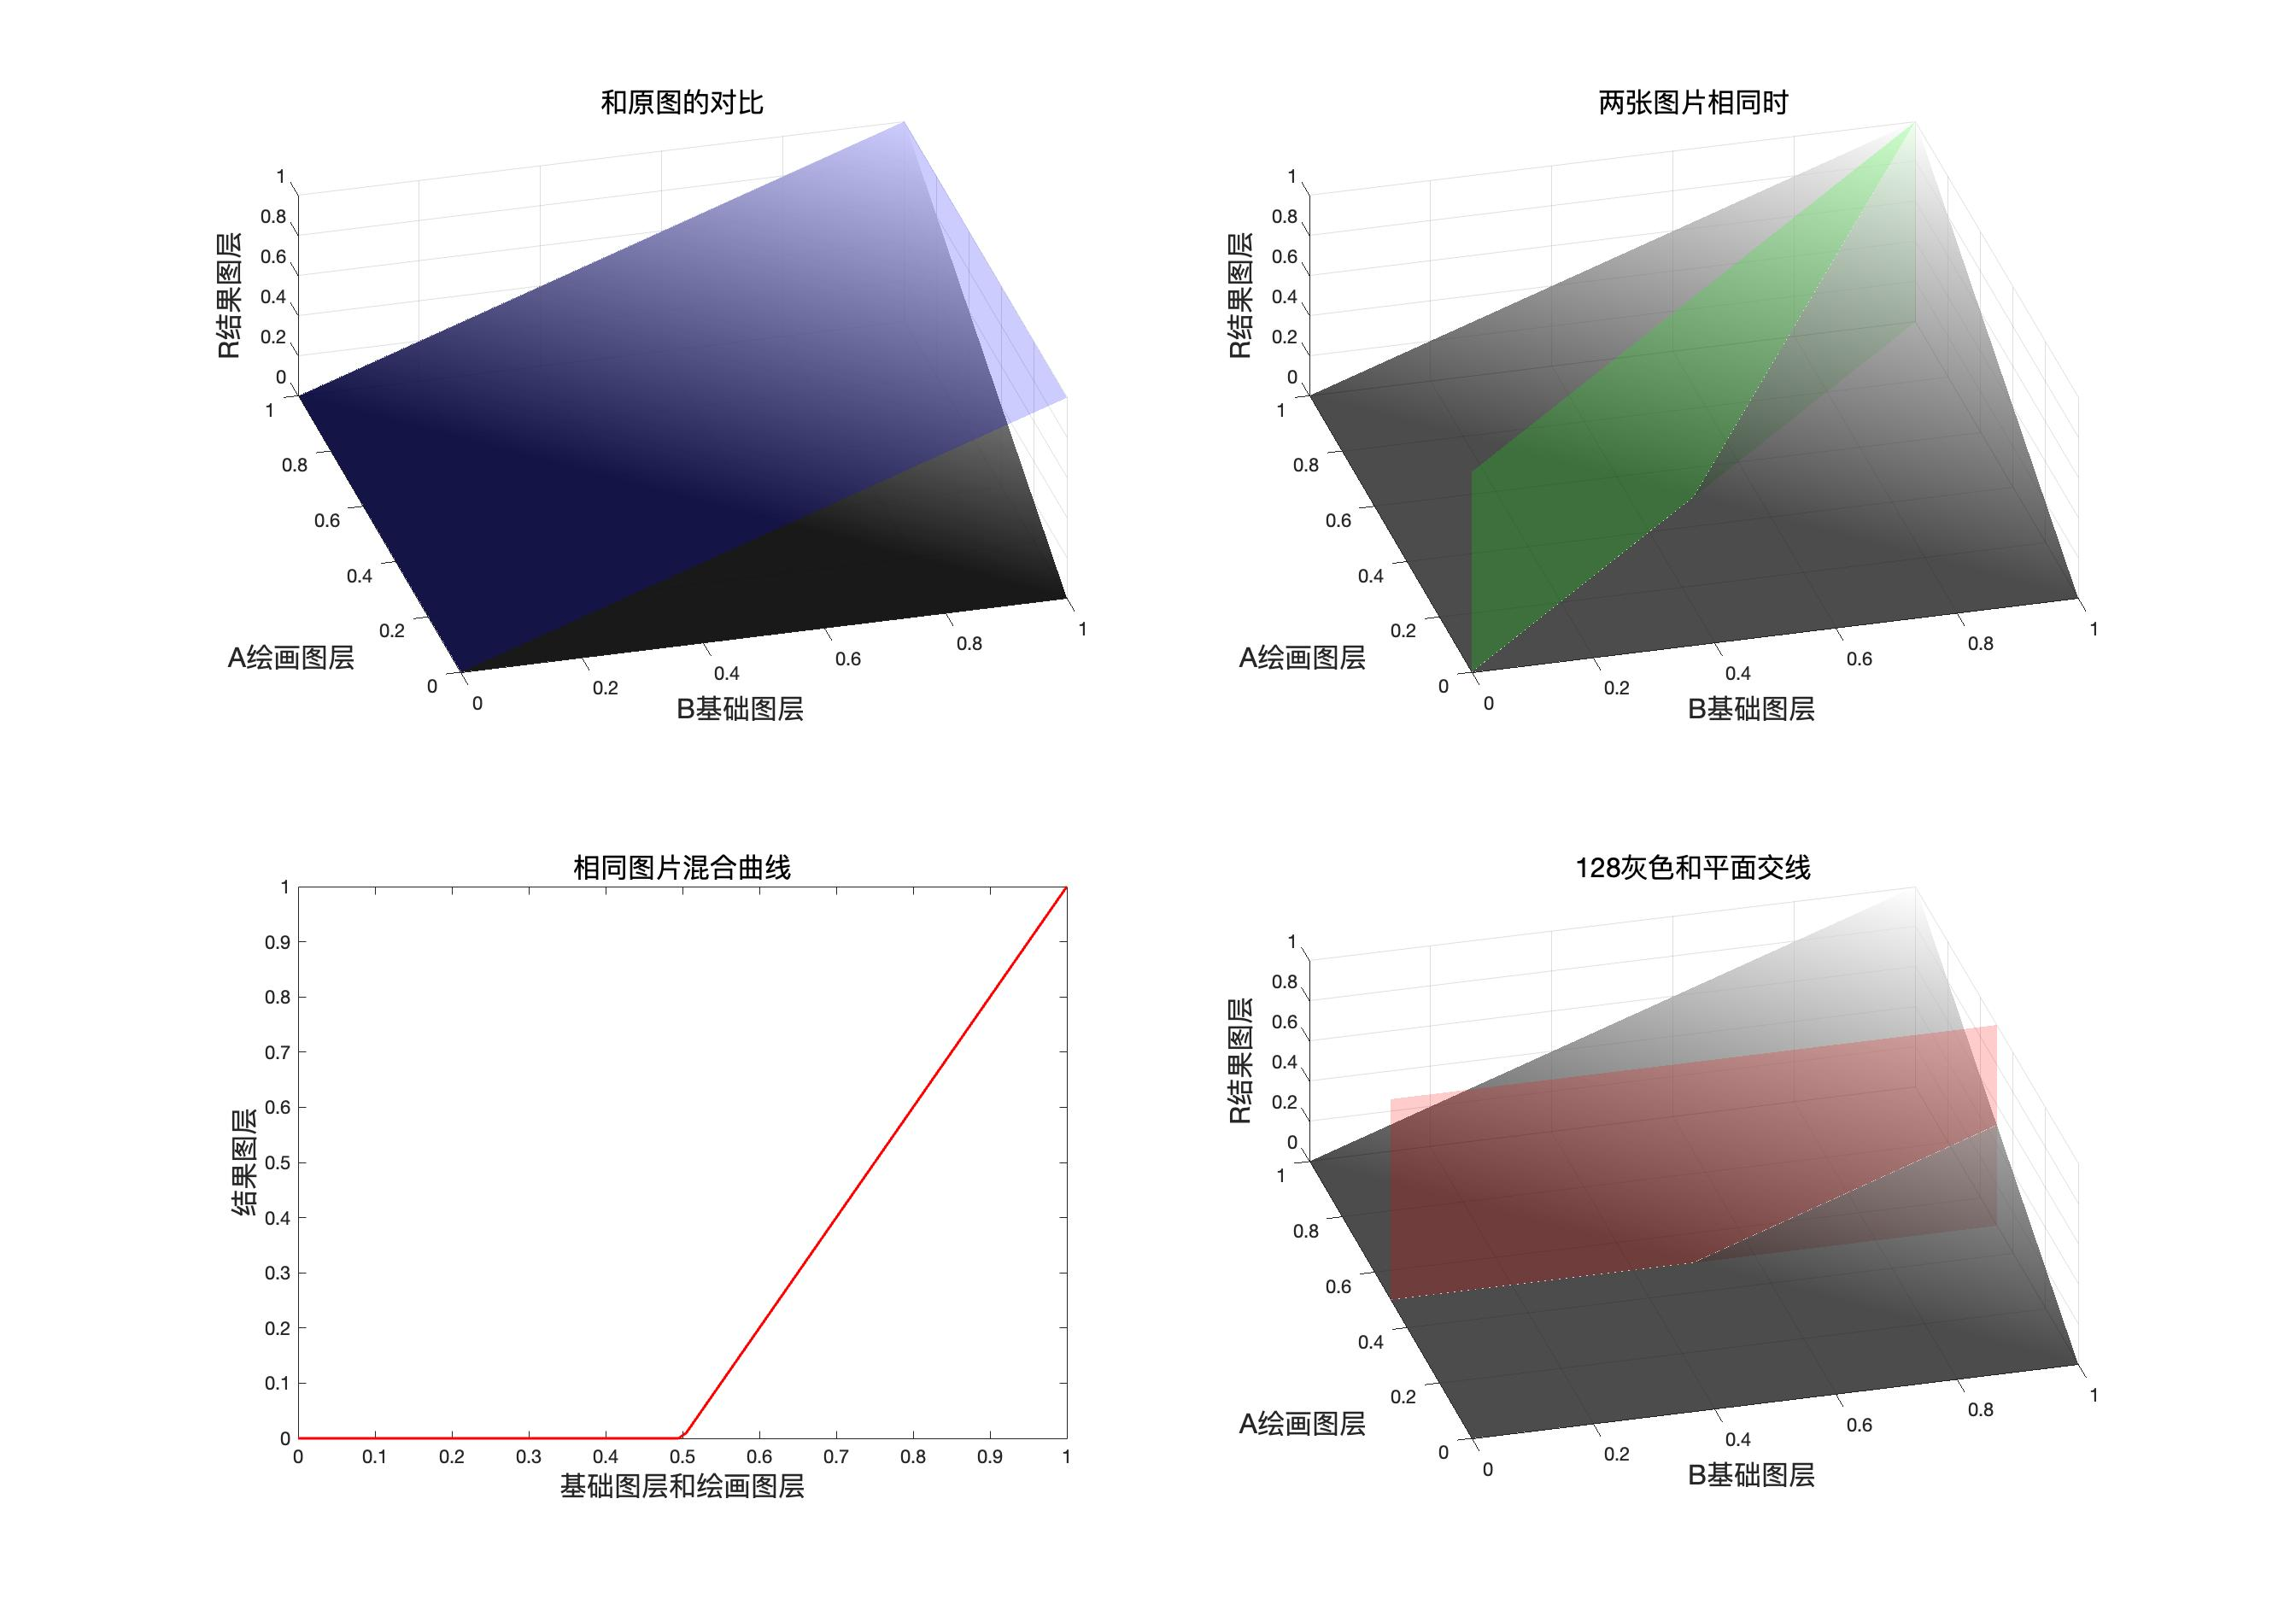
\includegraphics[width=\linewidth]{figure/线性加深.jpg}
	\caption{}
	\label{fig:}
\end{figure}


\subsection{ 同图曲线表达式}


\begin{equation}r=LinearBrun(b,b)=2\times b-1\end{equation}

\subsection{ 程序模拟该模式计算结果}

\begin{lstlisting}
	// 线性加深
	public static BlendColor LinearBurn(BlendColor colorBase, BlendColor colorBlend, double fill, double opacity) {
		double red = LinearBurnChannel(colorBase.red.get01Value(), colorBlend.red.get01Value(), fill);
		double green = LinearBurnChannel(colorBase.green.get01Value(), colorBlend.green.get01Value(), fill);
		double blue = LinearBurnChannel(colorBase.blue.get01Value(), colorBlend.blue.get01Value(), fill);
		return ColorUtils.Opacity(colorBase, new BlendColor(red *255, green* 255, blue * 255), opacity);
	}
	
	private static double LinearBurnChannel(double base, double blend, double fill) {
		return ColorUtils.round(base  (1 - blend) * fill, 1, 0);
	}
\end{lstlisting}



\begin{result}
 \item 线性加深(LinearBurn)    RGB[ 69.00,  35.60,  36.24]~ HSY[358.85,  33.40,  45.69]~ HSB[358.85,  48.41,  27.06]
\end{result}

\subsection{ 验证}

\begin{figure}[!htb]
	\centering
	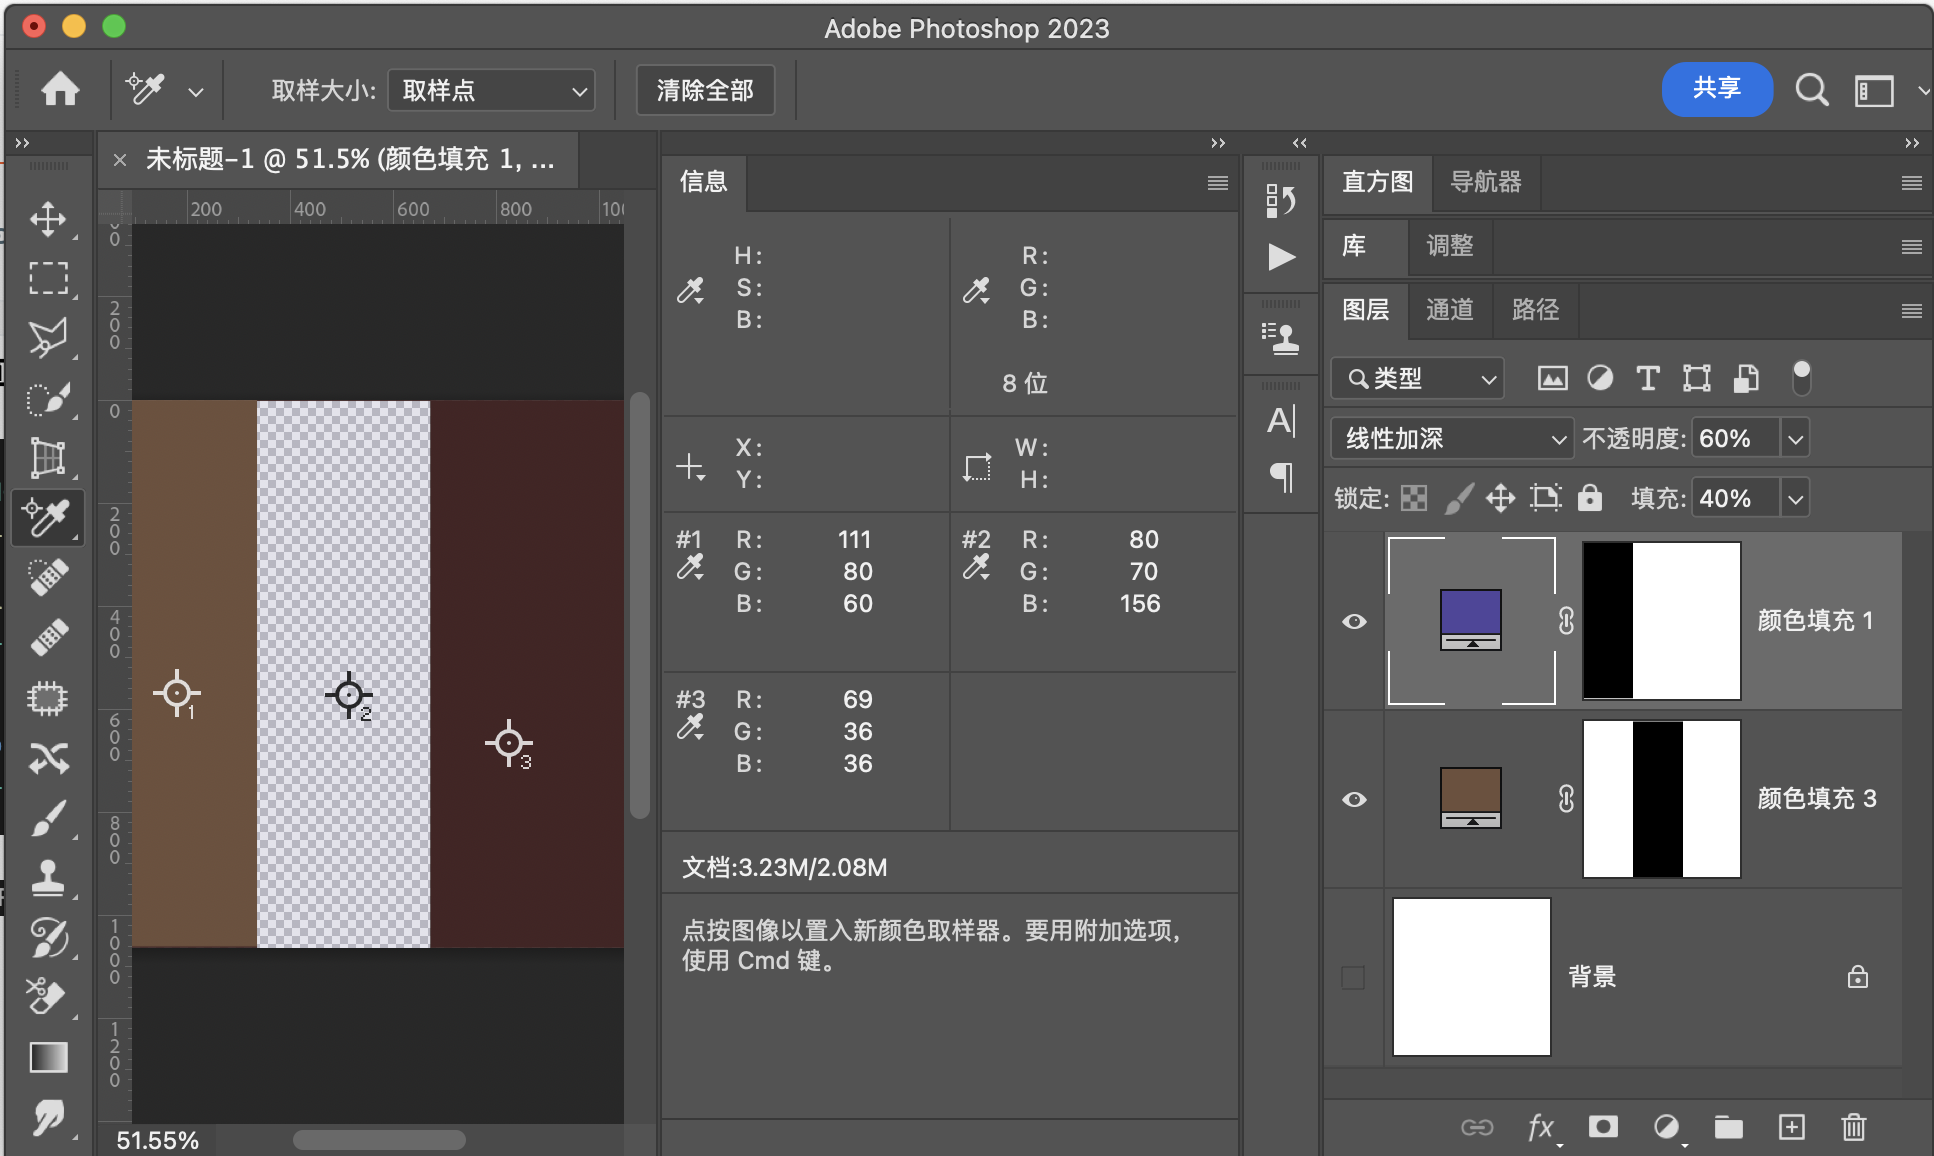
\includegraphics[width=\textwidth]{linearburn.png}
\end{figure}
%\subsection{ 用途示例}
%
%1:组成线性光
%
%2:添加光效可做滤镜
\newpage
\section{ 颜色加深ColorBurn}
此模式的本质是线性加深和混合图层相除,由此可以得知他可以和线性加深通过正片叠底转化。
\subsection{ 公式}
\begin{equation}\begin{aligned}&r=ColorBurn(b,a)=1-\dfrac{1-b}{1-(1-a)}\end{aligned}\end{equation}

这里之所以这么写,是因为后面要加入fill,也就是填充。


推导一下

\begin{equation}\begin{aligned}r&=ColorBurn(b,a)\\&=1-\dfrac{1-b}{1-(1-a)}=\dfrac{1-(1-a)-(1-b)}{1-(1-a)}=\dfrac{b-(1-a)}{1-(1-a)}\\&\\&=\dfrac{LinearBurn(b,a)}{1-(1-a)}=\dfrac{LinearBurn(b,a)}{a}\end{aligned}\end{equation}

\begin{notice}
\item 从这里可以看出,线性加深可以和颜色加深相互转换,通过划分和正片叠底。但是这里涉及到其他的混合模式,而非单纯负片,所以不把他们放到可以互相转化的分类中。
\end{notice}


\subsection{ 融合填充}


\begin{equation}r= Fill(b,a) =1-\dfrac{1-b}{1-(1-a)\times fill}\end{equation}

\subsection{ 融合不透明度}


\begin{equation}r=Opacity(b,a)=op\times Fill(b,a)+(1-op)\times b\end{equation}

\subsection{ 映射面和同图等效曲线}

颜色加深的映射面,同图面,同图曲线和中性灰平面


\subsection{ 同图曲线表达式}


\begin{equation} r= ColorBurn(b,b)=2-\dfrac{1}{b}\end{equation}

\subsection{ 两次负片转划分}


\begin{equation}\begin{aligned}&r=1-ColorBurn(1-b,a)\\&=1-(1-\dfrac{1-(1-b)}{a})=\dfrac{b}{a}\end{aligned}\end{equation}

\subsection{ 程序模拟该模式计算结果}
\begin{lstlisting}
	// 颜色加深
	public static BlendColor ColorBurn(BlendColor colorBase, BlendColor colorBlend, double fill, double opacity) {
		double red = ColorBurnChannel(colorBase.red.get01Value(), colorBlend.red.get01Value(), fill);
		double green = ColorBurnChannel(colorBase.green.get01Value(), colorBlend.green.get01Value(), fill);
		double blue = ColorBurnChannel(colorBase.blue.get01Value(), colorBlend.blue.get01Value(), fill);
		return ColorUtils.Opacity(colorBase, new BlendColor(red * 255, green * 255, blue * 255), opacity);
	}
	
	private static double ColorBurnChannel(double base, double blend, double fill) {
		return ColorUtils.round(1  Math.min(1, (1 - base) / ((1 - (1 - blend) * fill))), 1, 0);
	}
\end{lstlisting}

\begin{result}
\item 颜色加深(ColorBurn)     RGB[ 78.31,  37.07,  38.49]~ HSY[357.94,  41.24,  49.60]~ HSB[357.94,  52.66,  30.71]
\end{result}

\subsection{ 验证}
\begin{figure}[!htb]
	\centering
	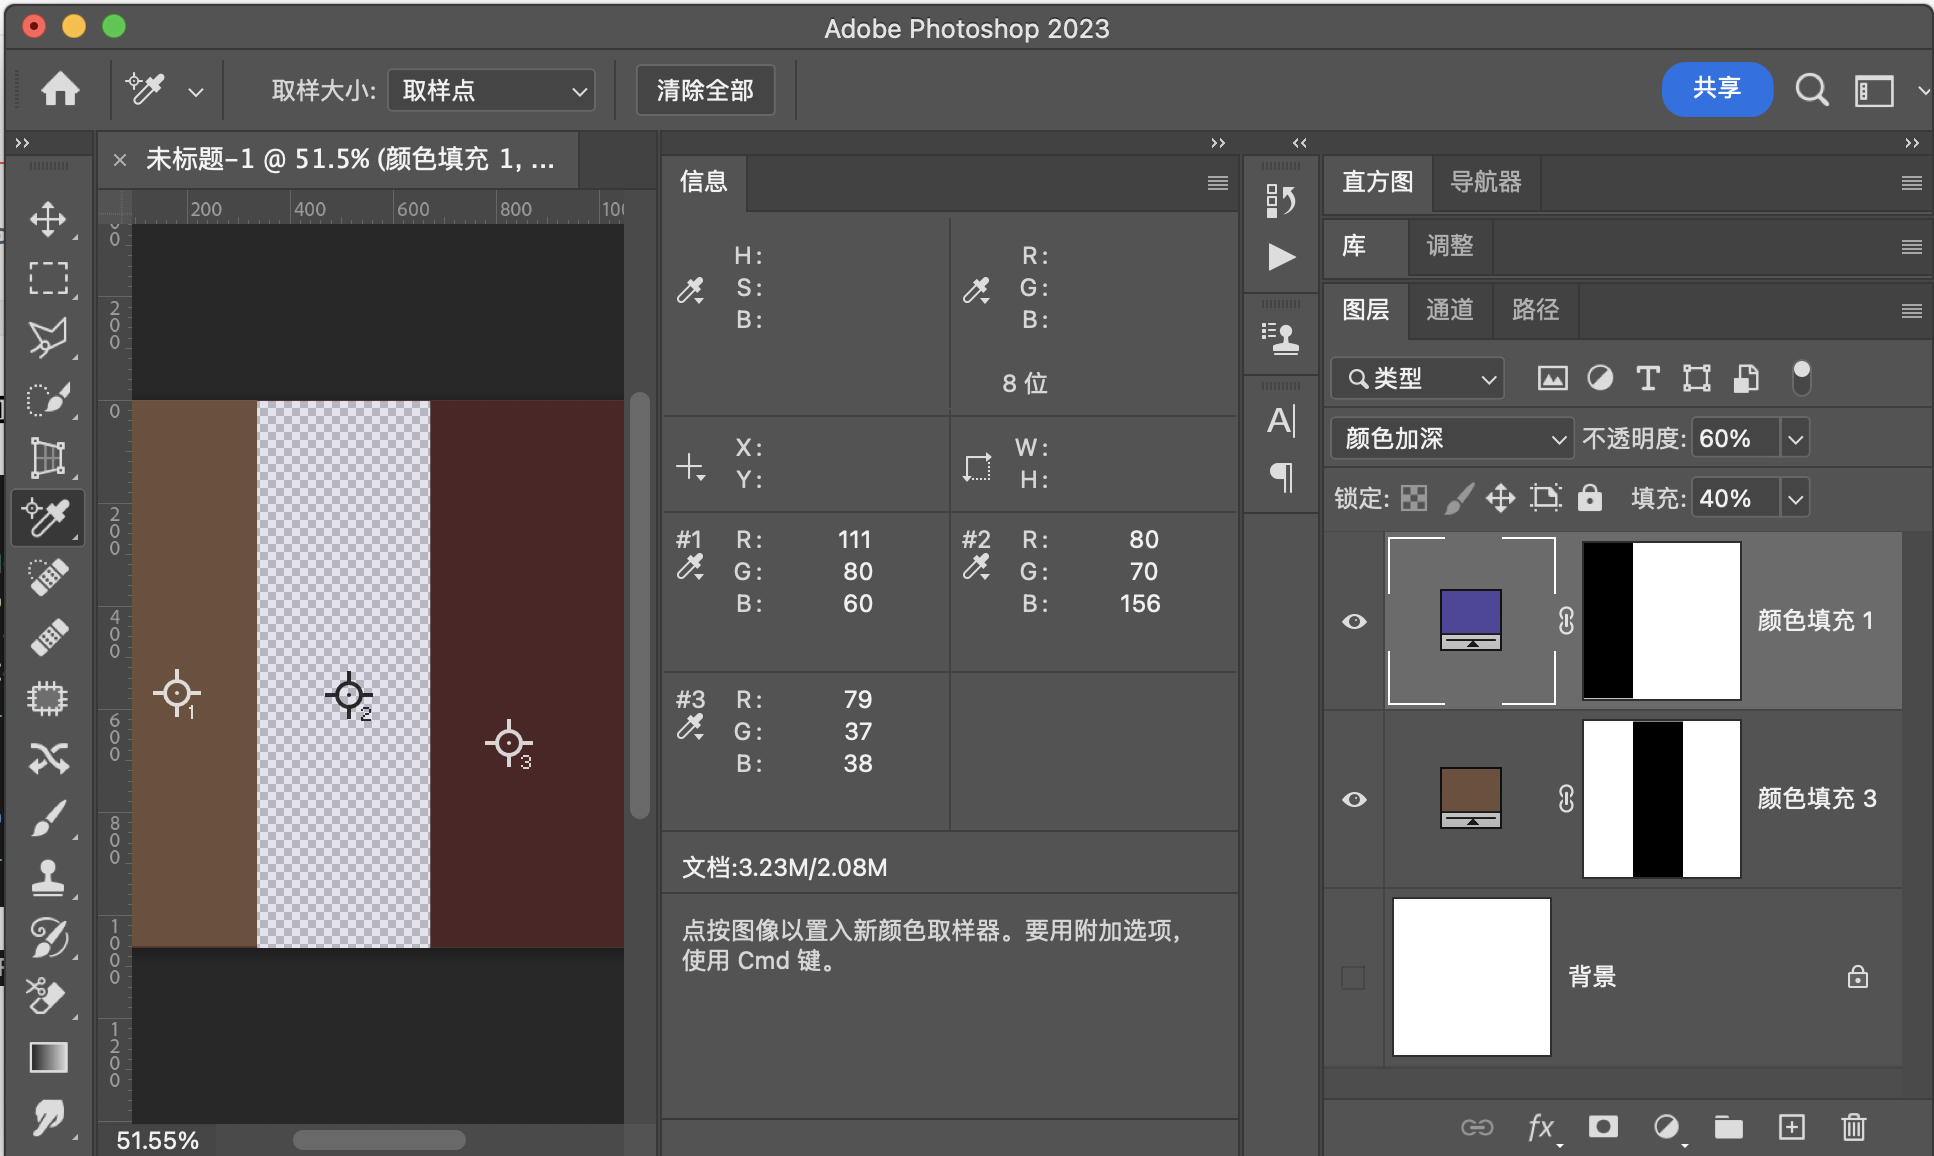
\includegraphics[width=\textwidth]{colorburn.png}
\end{figure}
%\subsection{ 用途示例}
%
%
%2:完成特殊光影效果,例如给太阳添加一些颜色或光晕,并且保留亮部细节,该模式的特点也是相对线性加深,可以保留底图的亮部细节。

\newpage
\section{ 深色Darker}

深色模式可以理解为变暗模式的加强变暗模式,或者是粗略的变暗模式,因为其不产生新的像素,就像溶解模式一样。
计算细节简单来说就是求和,比较大小,小的留下了,\text{若}求和的结果一样,就计算明度,明度小的留下了。

\subsection{ 公式}


\begin{equation}\begin{aligned}
	Pix_r &=Darker(Pix_b,Pix_a)\\&=\left\{\begin{aligned}&Pix_a && Sum(Pix_a)<Sum(Pix_b)\\&Pix_a&&  Sum(Pix_a)=Sum(Pix_b)\text{且}Lum(Pix_a)>Lum(Pix_b)\\&Pix_b&&  Sum(Pix_a)>Sum(Pix_b)\\&Pix_b&&  Sum(Pix_a)=Sum(Pix_b)\text{且}Lum(Pix_b)<Lum(Pix_a)\end{aligned}\right.
\end{aligned}\end{equation}
\begin{notice}
	\item 其中:\begin{flushleft}
		$Lum(Pix) = 0.3RC+0.59GC+0.11BC$\\
		$Sum(Pix) = RC+GC+BC$
	\end{flushleft}
\end{notice}
\subsection{ 融合填充}


\begin{equation}r= Fill(Pix_b,Pix_a) =fill\times Pix_r +(1-fill)\times Pix_b\end{equation}

\subsection{ 融合不透明度}


\begin{equation}r=Opacity(Pix_b,Pix_a)=op\times Fill(Pix_b,Pix_a)+(1-op)\times Pix_b \end{equation}

\subsection{ 映射面和同图等效曲线}

因为这里不是单一通道,所以不能给出单个通道的表达式。
\begin{equation}Pix_r=Pix_b\end{equation}
\newpage
\subsection{ 程序模拟该模式计算结果}

\begin{lstlisting}
	// 深色
	public static BlendColor Darker(BlendColor colorBase, BlendColor colorBlend, double fill, double opacity) {
			double sumBase = colorBase.red.value + colorBase.green.value + colorBase.blue.value;
			double sumBlend = (colorBlend.red.value + colorBlend.green.value + colorBlend.blue.value) * fill;
		
			if (sumBase == sumBlend) {
				if (colorBase.getLum() < colorBlend.getLum()) {
					double red = colorBase.red.get01Value();
					double green = colorBase.green.get01Value();
					double blue = colorBase.blue.get01Value();
					return ColorUtils.Opacity(colorBase, new BlendColor(red * 255, green * 255, blue * 255), opacity);
				} else {
				    double red = colorBase.red.get01Value() * (1 - fill) + colorBlend.red.get01Value() * fill;
					double green = colorBase.green.get01Value() * (1 - fill) + colorBlend.green.get01Value() * fill;
					double blue = colorBase.blue.get01Value() * (1 - fill) + colorBlend.blue.get01Value() * fill;
					return ColorUtils.Opacity(colorBase, new BlendColor(red * 255, green * 255, blue * 255), opacity);
			}
		}
			if (sumBase < sumBlend) {
				double red = colorBase.red.get01Value();
				double green = colorBase.green.get01Value();
				double blue = colorBase.blue.get01Value();
				return ColorUtils.Opacity(colorBase, new BlendColor(red * 255, green * 255, blue * 255), opacity);
		}
			double red = colorBase.red.get01Value() * (1 - fill) + colorBlend.red.get01Value() * fill;
			double green = colorBase.green.get01Value() * (1 - fill) + colorBlend.green.get01Value() * fill;
			double blue = colorBase.blue.get01Value() * (1 - fill) + colorBlend.blue.get01Value() * fill;
			return ColorUtils.Opacity(colorBase, new BlendColor(red * 255, green * 255, blue * 255), opacity);
	}
\end{lstlisting}

\begin{result}
\item 深    色(Darker)        RGB[103.56,  77.60,  83.04]~ HSY[347.43,  25.96,  85.99]~ HSB[347.43,  25.07,  40.61]
\end{result}
\newpage
\subsection{ 验证}

\begin{figure}[!htb]
	\centering
	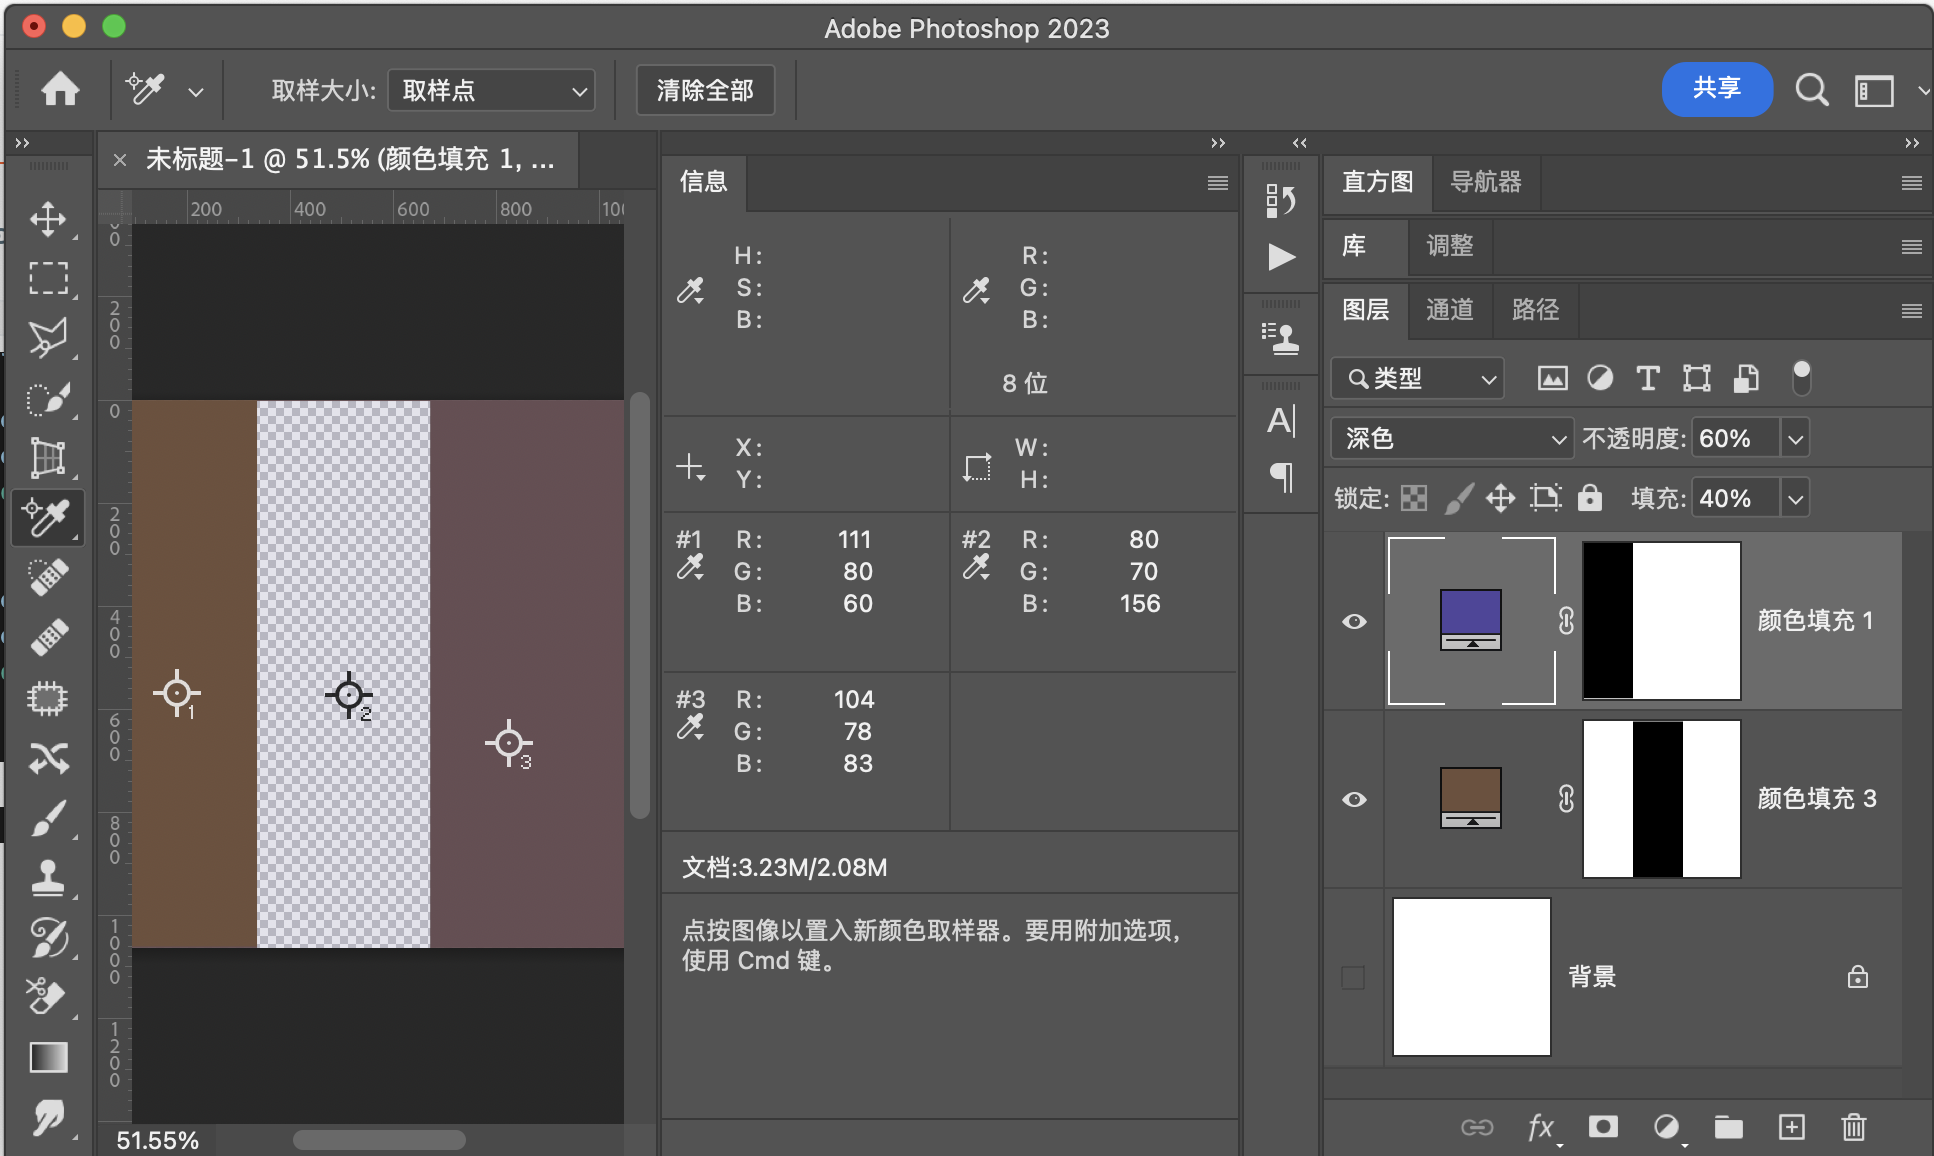
\includegraphics[width=\linewidth]{figure/darker}
	\caption{深色模式验证结果}
	\label{fig:darker}
\end{figure}


%
%\subsection{ 用途示例}
%
%用于替换图中某些像素点,一般用于两张十分相似的图片的融合,比如连拍,延时摄影的一组照片融合成一张图。

\chapter{变亮组}
\begin{introduction}
	\item  变亮组是变暗组的相反模式,并且都可以通过负片操作来实现相互转换
	变亮组的本质就是以混合图层的像素为参数,对原图层像素的数值进行增大,数值增大了,图片就变亮了。如果混合图层中像素点的通道值时0,则此时该通道的计算结果和原图一致。
\end{introduction}


\section{ 变亮Lighten}

变亮模式和变暗模式相反,变暗时取最小值,变亮就是取最大值,具体做法就是取原图层和混合图层像素点中三个通道各自的最大值,保留最大值组成的像素作为结果像素。

\subsection{ 公式}


\begin{equation}r=Lighten(b,a)=Max(b,a)\end{equation}

\subsection{ 融合填充}


\begin{equation}r= Fill(b,a) =fill\times Lighten(b,a)+(1-fill)\times b\end{equation}

\subsection{ 融合不透明度}


\begin{equation}r=Opacity(b,a)=op\times Fill(b,a)+(1-op)\times b\end{equation}

\subsection{ 三次负片操作相互转换}


\begin{equation}\begin{aligned}
	r&=Lighten(b,a)\\&=1-Min(1-b,1-a)\\&= 1-Darken(1-b,1-a)
\end{aligned}\end{equation}
也就是说,三次负片操作可以实现变暗模式和变亮模式的相互转换
\newpage
\subsection{ 映射面和同图等效曲线}
% TODO: \usepackage{graphicx} required
\begin{figure}[h!]
	\centering
	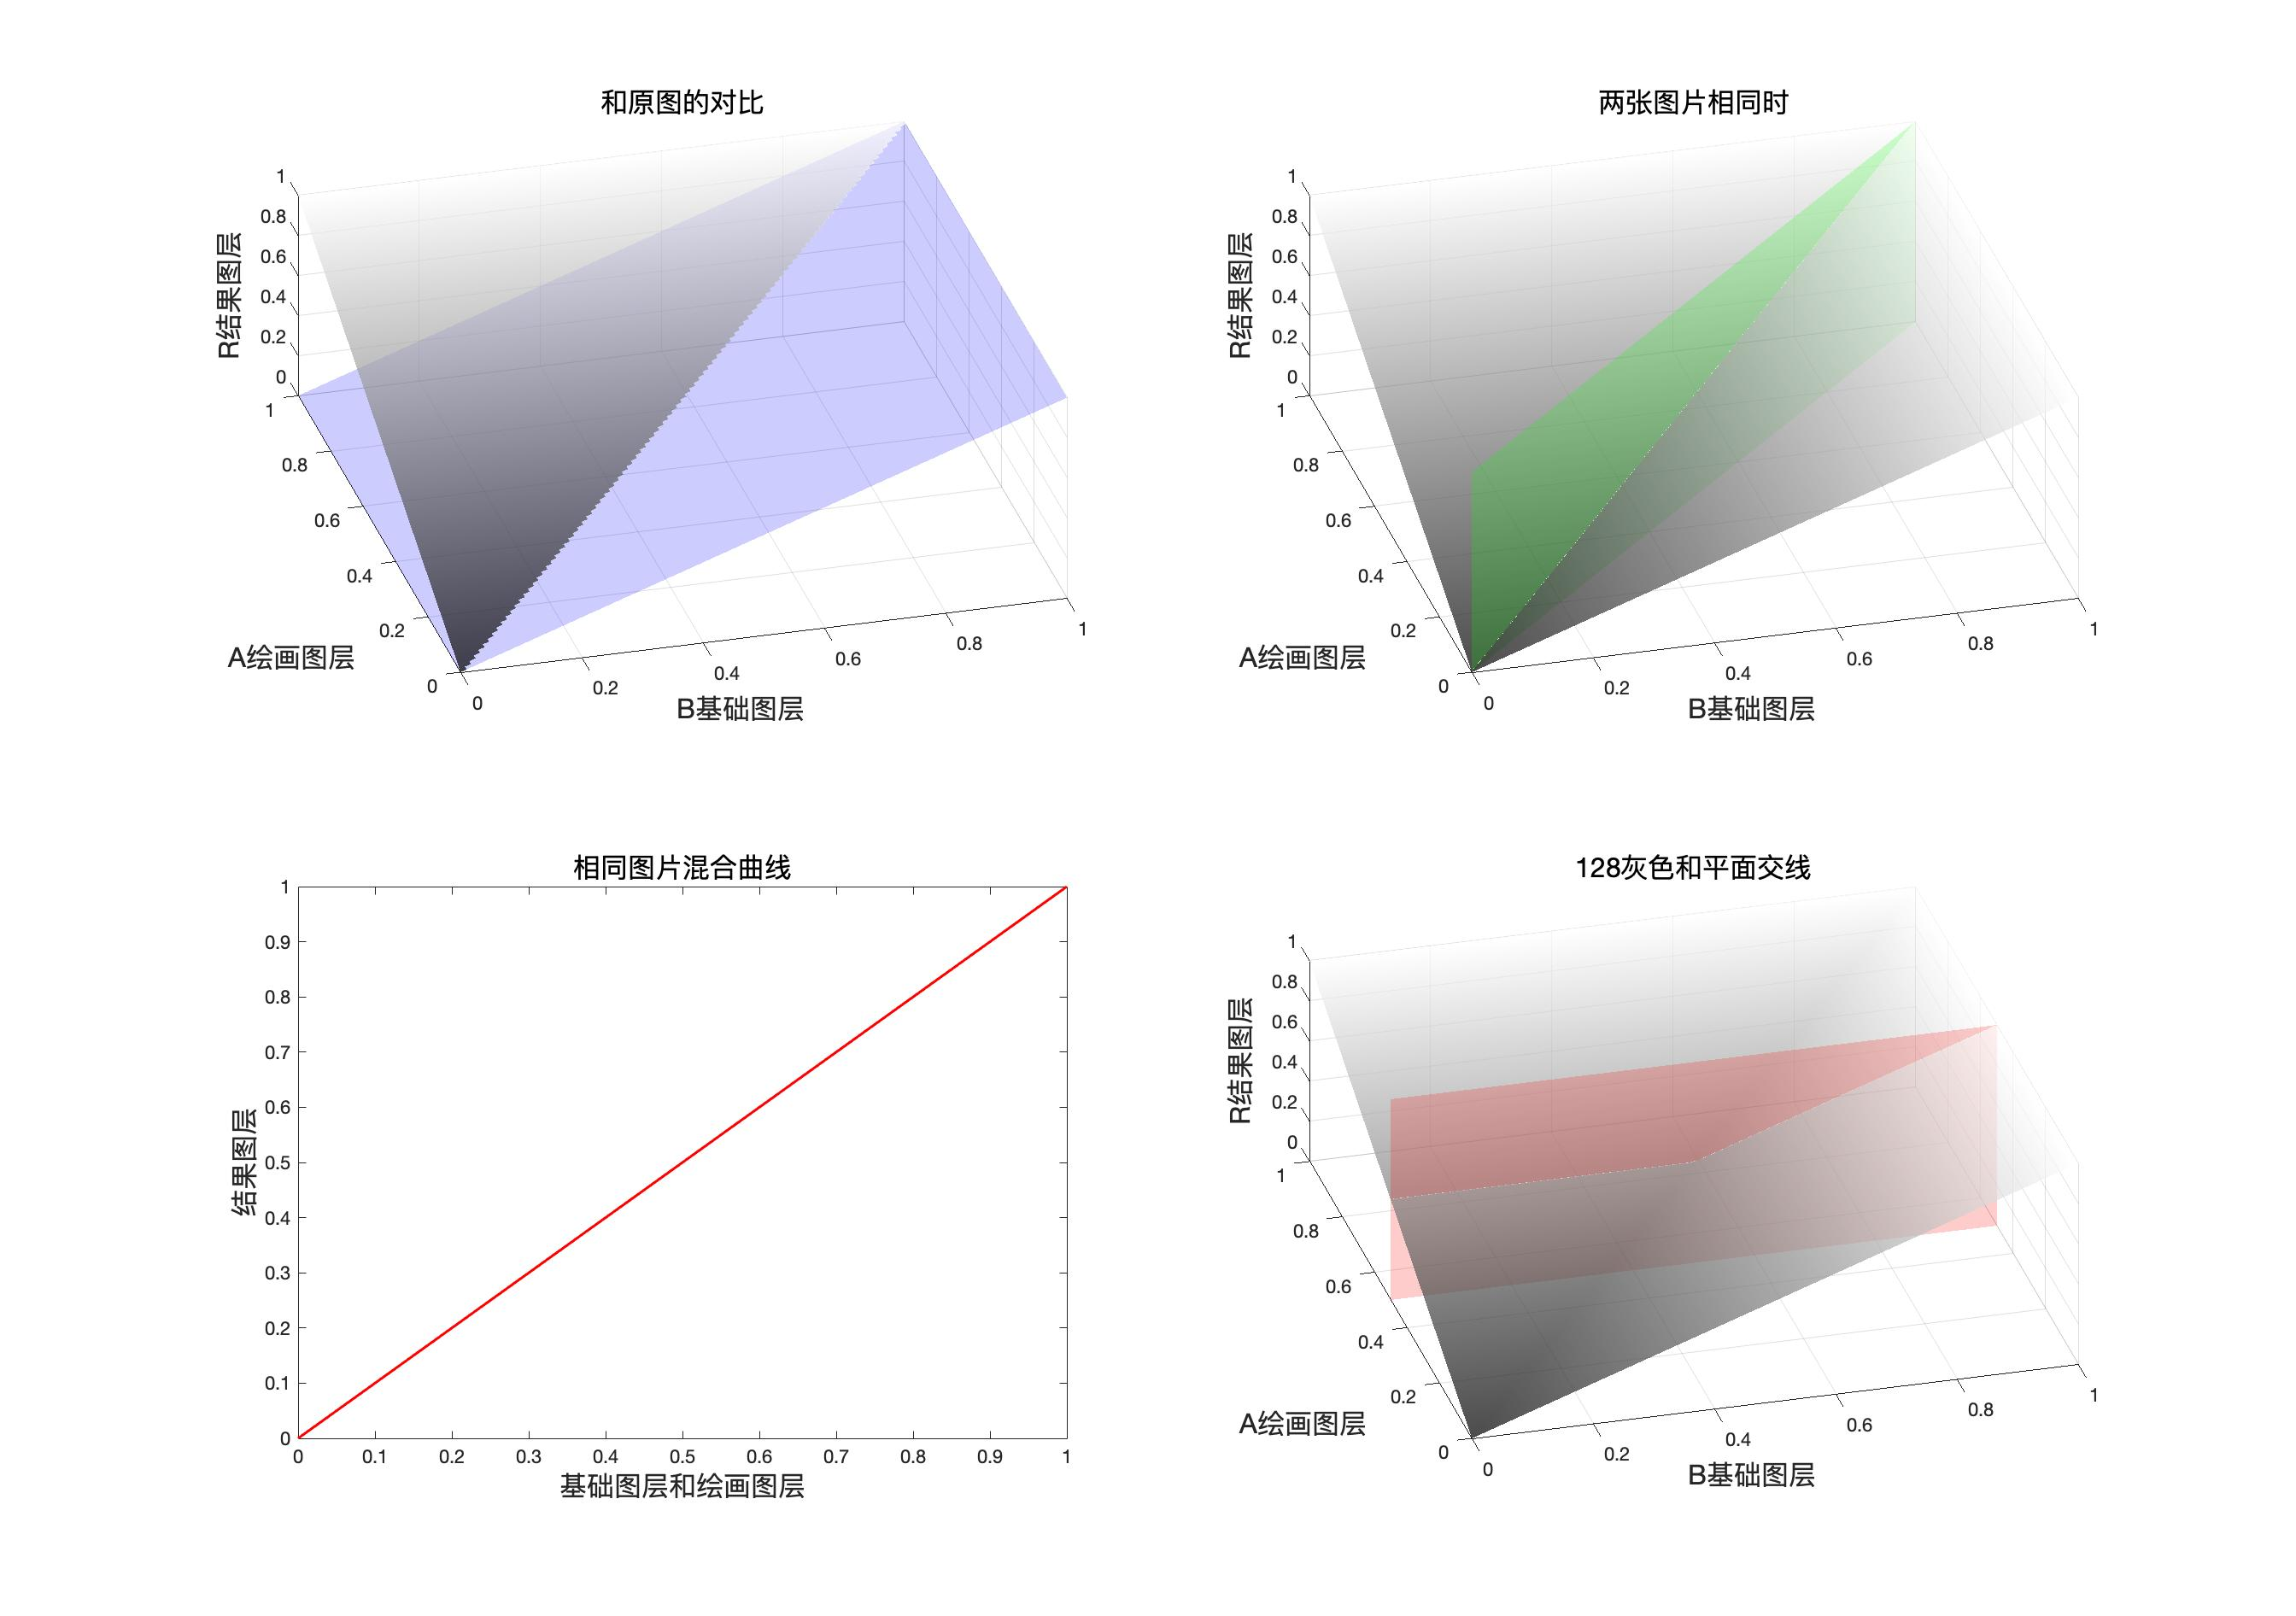
\includegraphics[width=\linewidth]{figure/变亮}
	\caption{}
	\label{fig:}
\end{figure}


\subsection{ 程序模拟该模式计算结果}

\begin{lstlisting}
	// 变亮模式
	public static BlendColor Lighten(BlendColor colorBase, BlendColor colorBlend, double fill, double opacity) {
		double red = LightenChannel(colorBase.red.get01Value(), colorBlend.red.get01Value(), fill);
		double green = LightenChannel(colorBase.green.get01Value(), colorBlend.green.get01Value(), fill);
		double blue = LightenChannel(colorBase.blue.get01Value(), colorBlend.blue.get01Value(), fill);
		return ColorUtils.Opacity(colorBase, new BlendColor(red * 255, green * 255, blue * 255), opacity);
	}
	
	private static double LightenChannel(double base, double blend, double fill) {
		return Math.max(base, blend * fill) * fill + (1 - fill) * base;
	}
	
\end{lstlisting}


\begin{result}
\item 变    亮(Lighten)       RGB[111.00,  80.00,  83.04]~ HSY[354.12,  31.00,  89.63]~ HSB[354.12,  27.93,  43.53]
\end{result}

\subsection{ 验证}
% TODO: \usepackage{graphicx} required
\begin{figure}[h!]
	\centering
	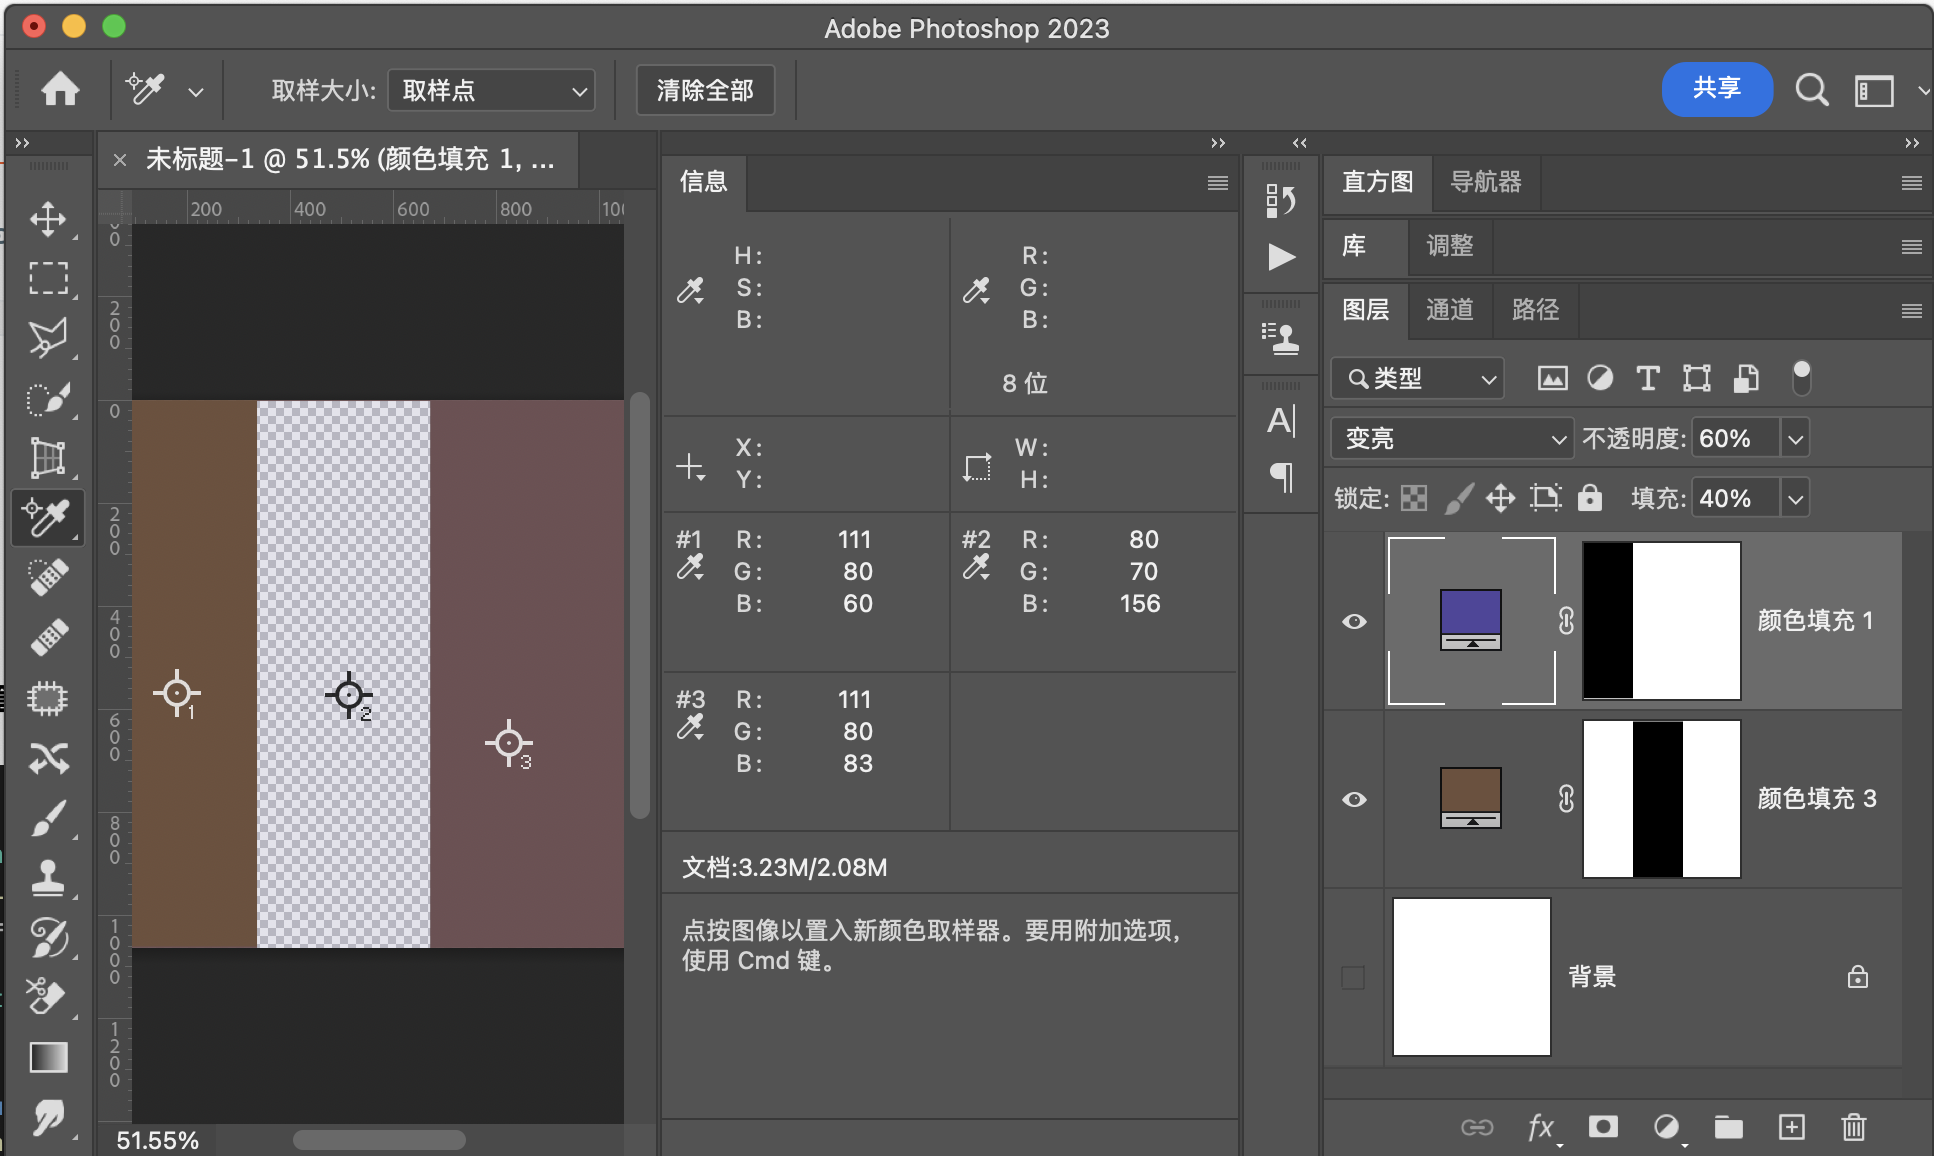
\includegraphics[width=\linewidth]{figure/lighten}
	\caption{}
	\label{fig:lighten}
\end{figure}
%
%\subsection{ 用途示例}
%
%1:组成叠加和强光
%2:保留通道中较大的值,并且组成新的像素,可用于将背景较暗或相似但是部分不相同的图片融合。相当于做了一个复杂的通道蒙版,并且这个蒙版非常精确,精确到通道。

\newpage
\section{ 滤色Screen}

滤色时正片叠底的一种负片组合,和变暗变亮一样可以通过三次负片操作相互转换。

\subsection{ 公式}


\begin{equation}r=Screen(b,a)=1-(1-b)(1-a)\end{equation}

\subsection{ 融合填充}


\begin{equation}r= Fill(b,a) =fill\times Screen(b,a)+(1-fill)\times b\end{equation}

\subsection{ 融合不透明度}


\begin{equation}r=Opacity(b,a)=op\times Fill(b,a)+(1-op)\times b\end{equation}

\subsection{ 三次负片操作相互转换}


\begin{equation}\begin{aligned}
	r&=Screen(b,a)\\&=1-(1-b)(1-a)\\&= 1 -Multipy(1-b,1-a)
\end{aligned}\end{equation}
\newpage
\subsection{ 映射面和同图等效曲线}
% TODO: \usepackage{graphicx} required
\begin{figure}[h!]
	\centering
	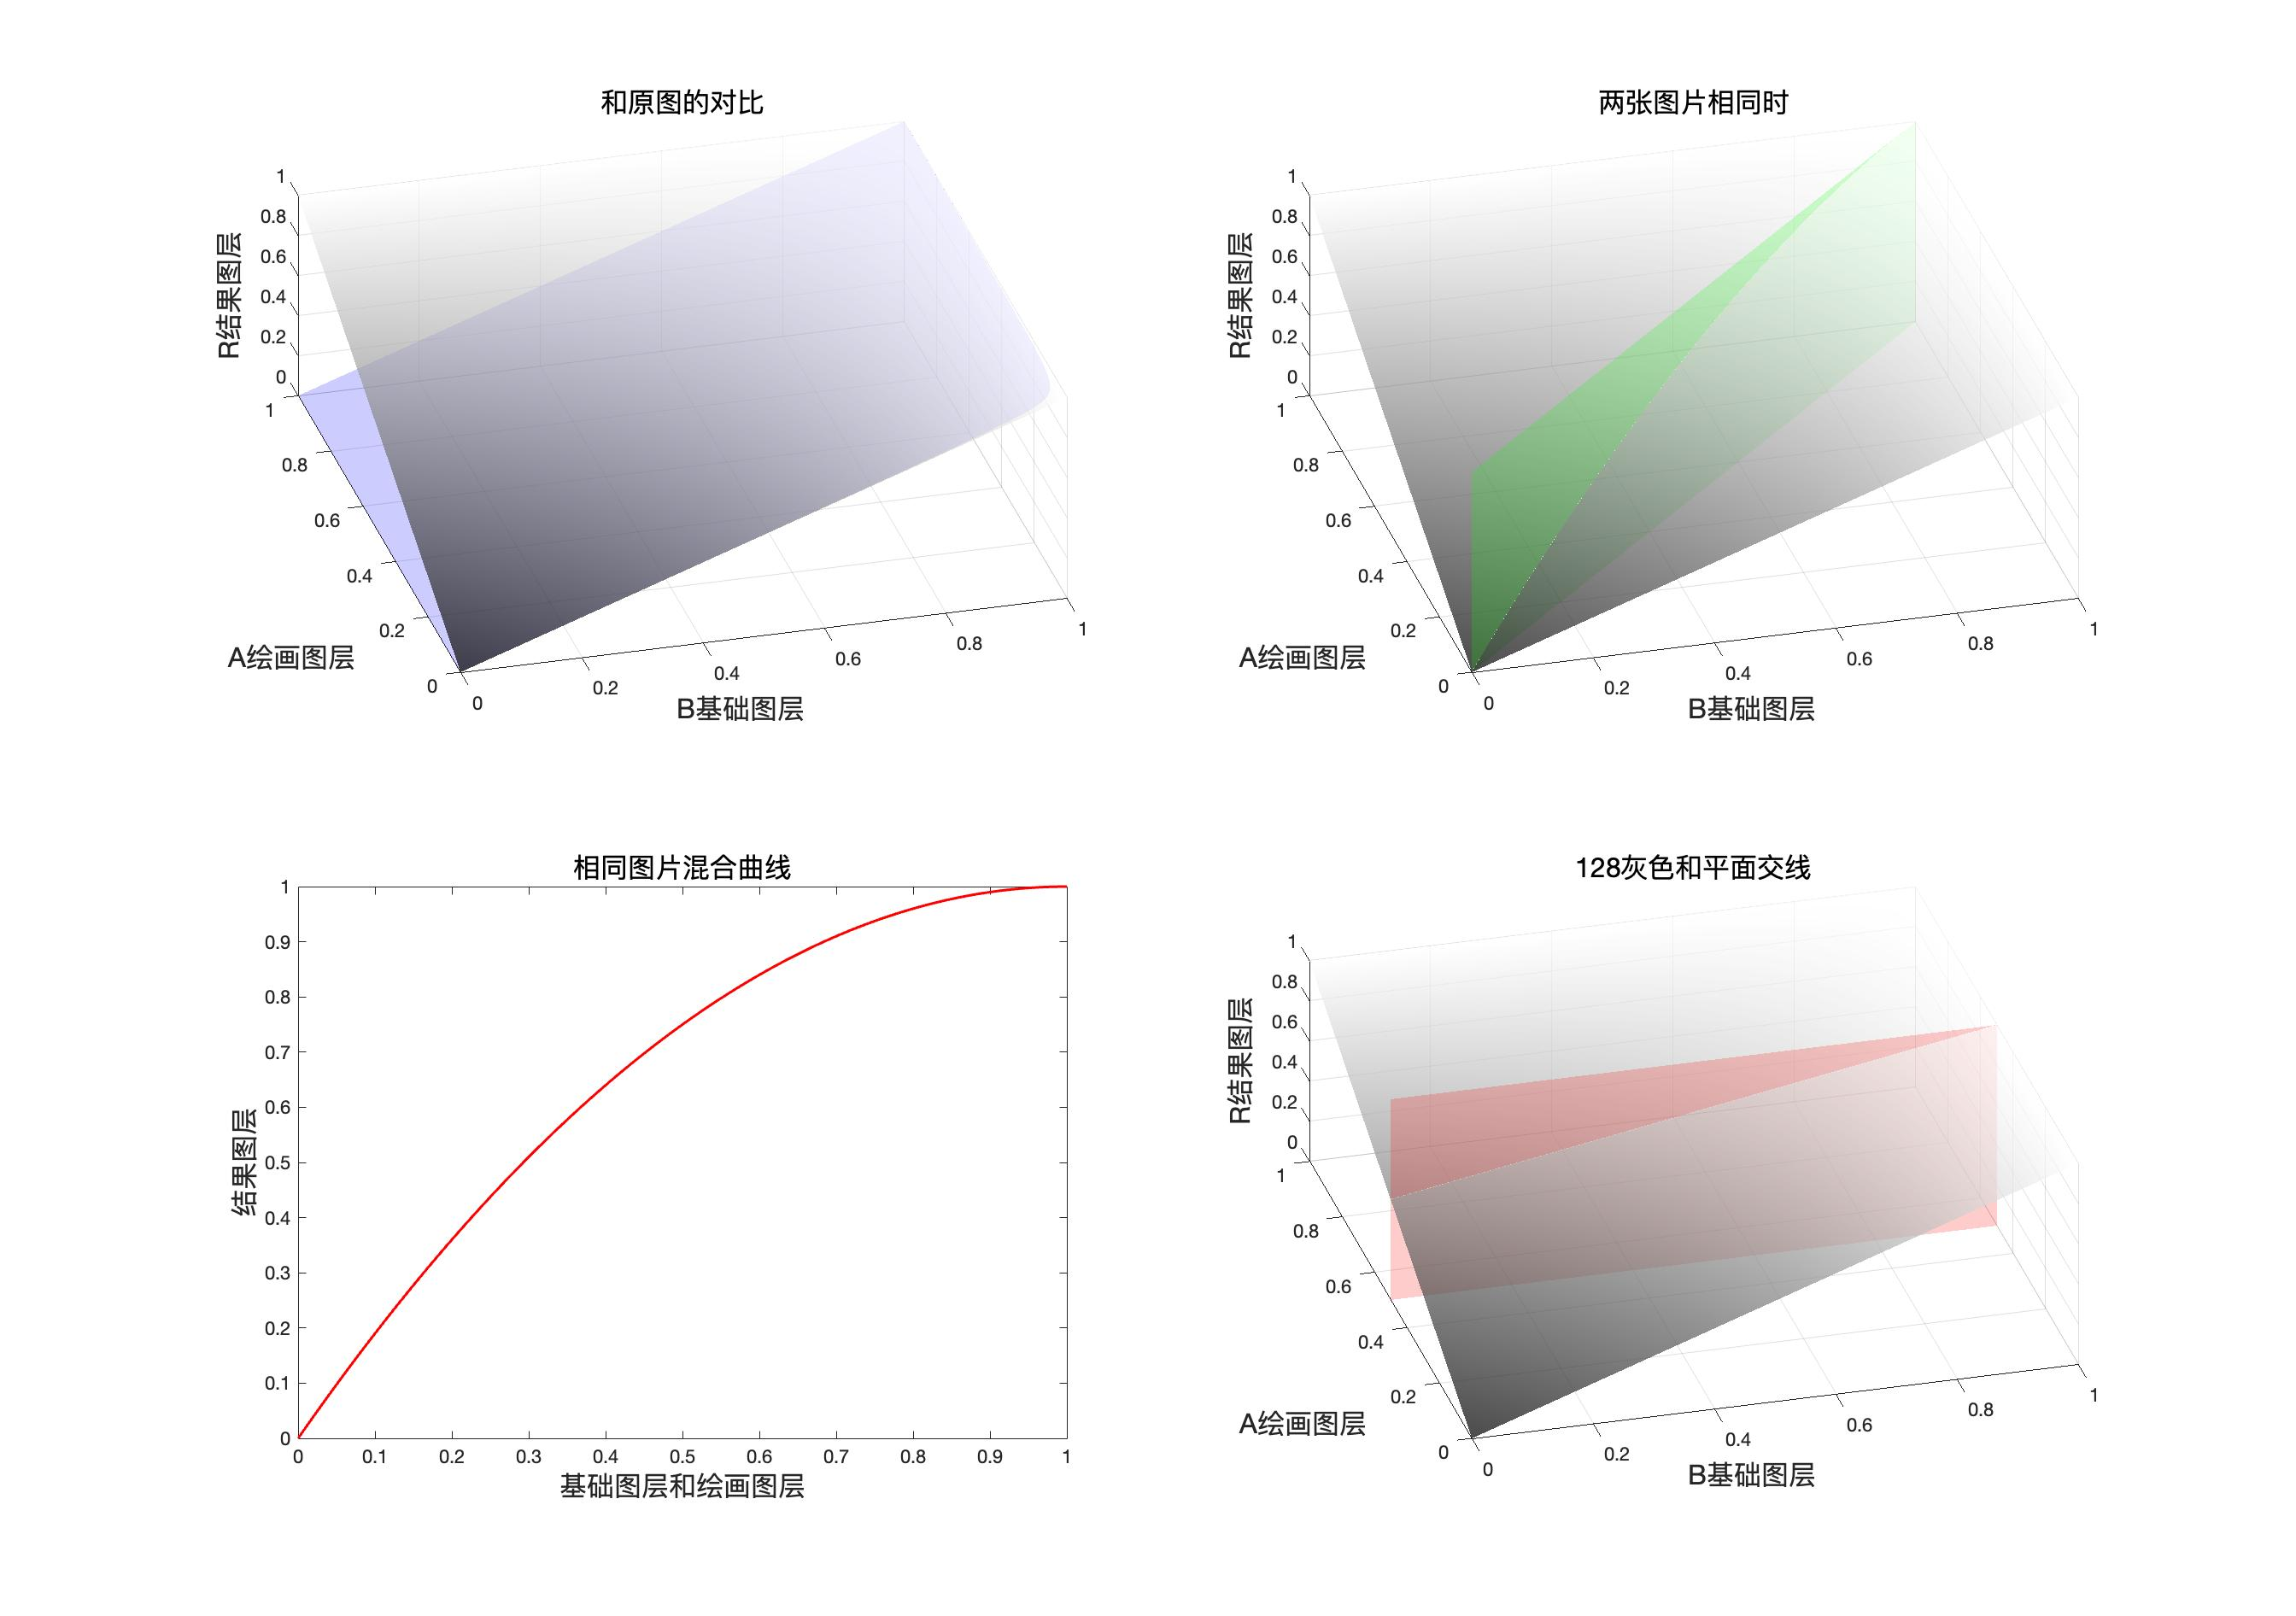
\includegraphics[width=\linewidth]{figure/滤色}
	\caption{}
	\label{fig:}
\end{figure}


\subsection{ 程序模拟该模式计算结果}

\begin{lstlisting}
	// 滤色
	public static BlendColor Screen(BlendColor colorBase, BlendColor colorBlend, double fill, double opacity) {
		double red = ScreenChannel(colorBase.red.get01Value(), colorBlend.red.get01Value(), fill);
		double green = ScreenChannel(colorBase.green.get01Value(), colorBlend.green.get01Value(), fill);
		double blue = ScreenChannel(colorBase.blue.get01Value(), colorBlend.blue.get01Value(), fill);
		return ColorUtils.Opacity(colorBase, new BlendColor(red * 255, green * 255, blue * 255), opacity);
	}
	
	private static double ScreenChannel(double base, double blend, double fill) {
		return (1 - (1 - base) * (1 - blend)) * fill + (1 - fill) * base;
	}
\end{lstlisting}


\begin{result}
\item 滤    色(Screen)        RGB[121.84,  91.53,  88.63]~ HSY[5.24,  33.21, 100.30  ]~ HSB[  5.24,  27.26,  47.78]
\end{result}

\subsection{ 验证}
% TODO: \usepackage{graphicx} required
\begin{figure}[h!]
	\centering
	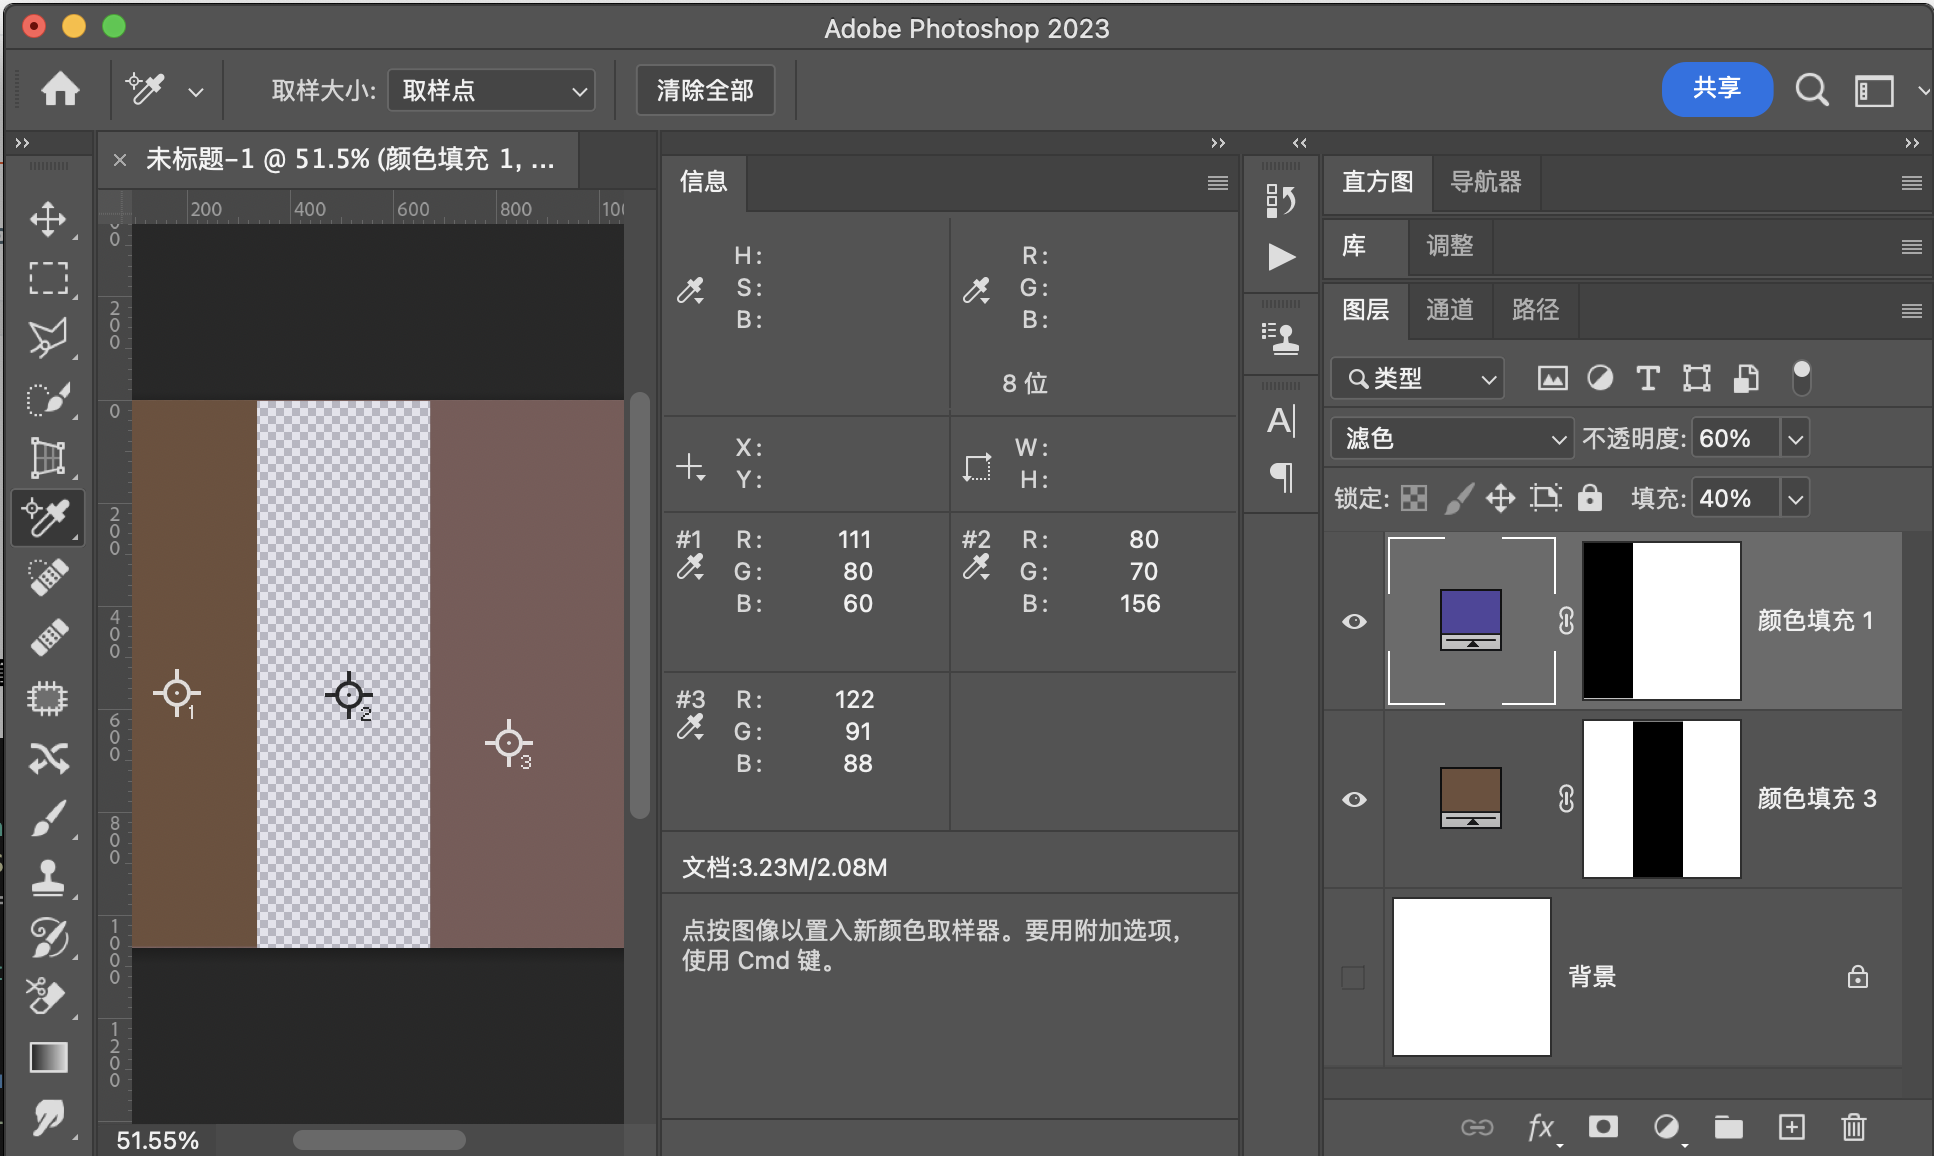
\includegraphics[width=\linewidth]{figure/screen}
	\caption{}
	\label{fig:screen}
\end{figure}

%
%\subsection{ 用途示例}
%
%1:组成叠加模式和强光模式
%
%2:扣除黑色背景

\newpage
\section{ 线性减淡LinearDodge}

线性减淡就是让原图和混合图层做加法
他和线性加深也是可以互相转化的

\subsection{ 公式}


\begin{equation}r=LinearDodge(b,a)=b+a\end{equation}

\subsection{ 融合填充}


\begin{equation}r= Fill(b,a) =b+a\times fill \end{equation}

\subsection{ 融合不透明度}


\begin{equation}r=Opacity(b,a)=op\times Fill(b,a)+(1-op)\times b\end{equation}

\subsection{ 三次负片操作相互转换}

\begin{equation}
\begin{aligned}
	r&=LinearDodge(b,a)= 1-LinearBurn(1-b,1-a)\\& = 1-(1-b+1-a-1)=b+a
\end{aligned}
\end{equation}

\subsection{ 映射面和同图等效曲线}
% TODO: \usepackage{graphicx} required
\begin{figure}[h!]
	\centering
	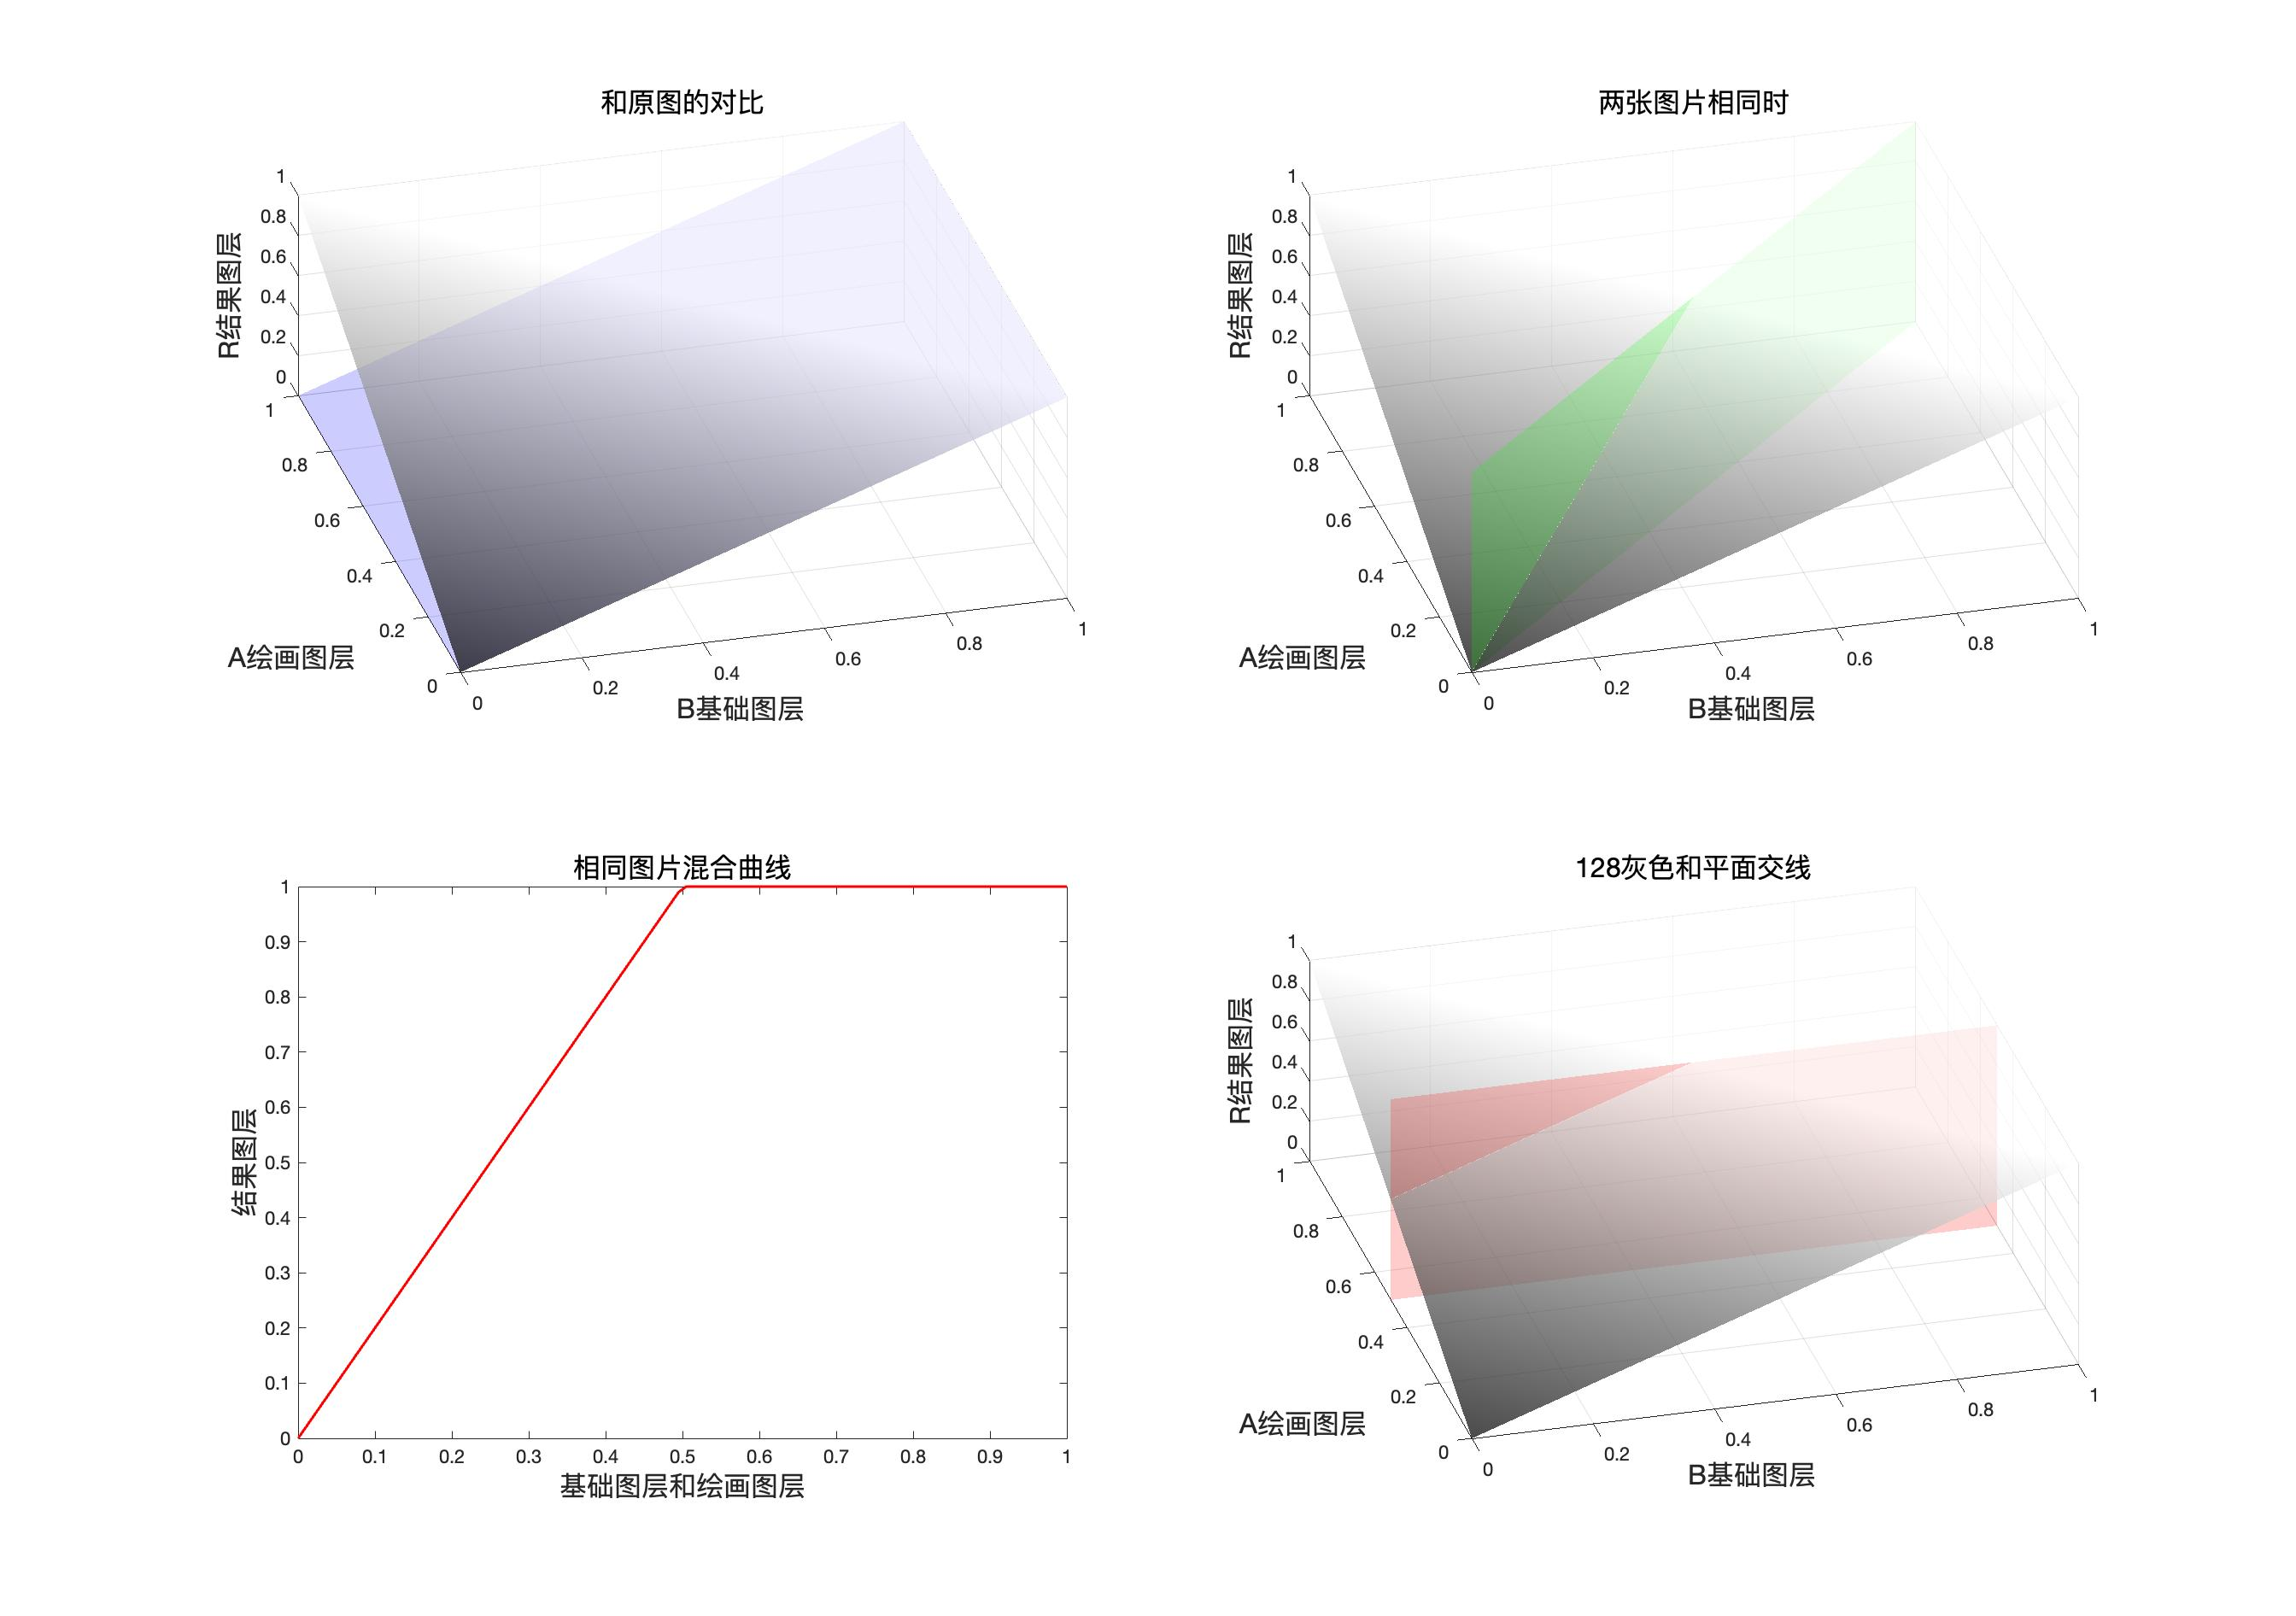
\includegraphics[width=\linewidth]{figure/线性减淡.jpg}
	\caption{}
	\label{fig:}
\end{figure}


\subsection{ 程序模拟该模式计算结果}

\begin{lstlisting}
	// 线性减淡
	public static BlendColor LinearDodge(BlendColor colorBase, BlendColor colorBlend, double fill, double opacity) {
		
		double red = LinearDodgeChannel(colorBase.red.get01Value(), colorBlend.red.get01Value(), fill);
		double green = LinearDodgeChannel(colorBase.green.get01Value(), colorBlend.green.get01Value(), fill);
		double blue = LinearDodgeChannel(colorBase.blue.get01Value(), colorBlend.blue.get01Value(), fill);
		return ColorUtils.Opacity(colorBase, new BlendColor(red * 255, green * 255, blue * 255), opacity);
	}
	
	private static double LinearDodgeChannel(double base, double blend, double fill) {
		return ColorUtils.round(base + blend * fill, 1, 0);
	}
	
\end{lstlisting}



\begin{result}
\item 线性减淡(LinearDodge)   RGB[130.20,  96.80,  97.44]~ HSY[358.85,  33.40, 106.89]~ HSB[358.85,  25.65,  51.06]
\end{result}

\subsection{ 验证}
% TODO: \usepackage{graphicx} required
\begin{figure}[h!]
	\centering
	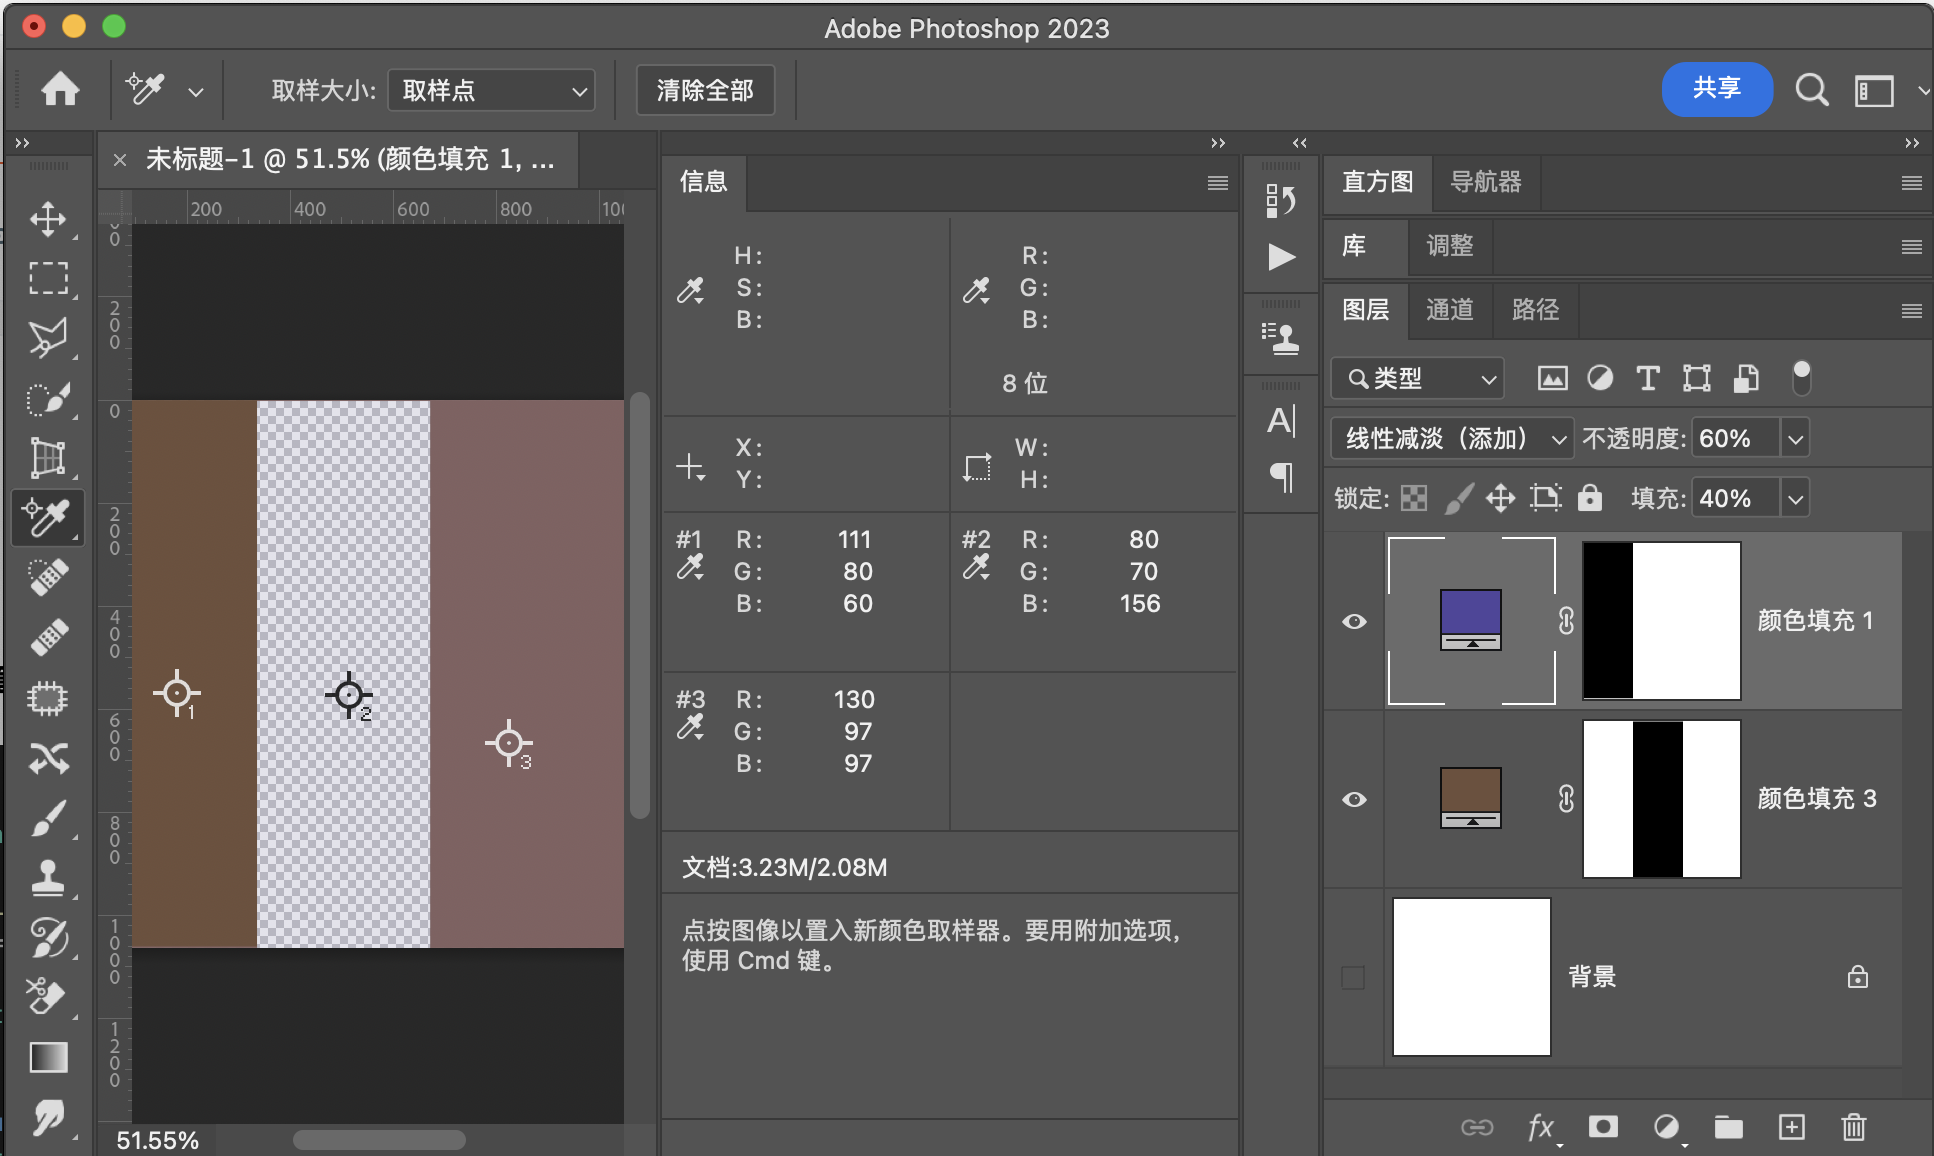
\includegraphics[width=\linewidth]{figure/linearndodge}
	\caption{}
	\label{fig:linearndodge}
\end{figure}

%
%\subsection{ 用途示例}
%
%1:组成线性光
%
%2: 制作特殊光效

\newpage
\section{ 颜色减淡ColorDodge}

颜色减淡可以由颜色加深通过三次负片转化,颜色减淡也可以转化为划分,通过一次负片可以实现

\subsection{ 公式}


\begin{equation}
	r=ColorDodge(b,a)=\dfrac{b}{1-a}
	\end{equation}

\subsection{ 融合填充}


\begin{equation}
	r= Fill(b,a) =\dfrac{b}{1-a\times fill}
	 \end{equation}

\subsection{ 融合不透明度}


\begin{equation}r=Opacity(b,a)=op\times Fill(b,a)+(1-op)\times b\end{equation}
\subsection{结合负片操作和其他模式互转}
结合负片操作之后,我们可以让颜色减淡和颜色加深以及划分相互转换.
\subsubsection{ 三次负片操作转换为颜色加深}


\begin{equation}\begin{aligned}
	r&=ColorDodge(b,a)= 1-ColorBurn(1-b,1-a)\\& =1-(1-\dfrac{1-(1-b)}{1-(1-(1-a))})=\dfrac{b}{1-a}
\end{aligned}\end{equation}

\subsubsection{ 一次负片转为划分}


\begin{equation}\begin{aligned}
	r&=ColorDodge(b,1-a)\\&= \dfrac{b}{1-1+a}=\dfrac{b}{a}
\end{aligned}\end{equation}

\subsection{ 映射面和同图等效曲线}
% TODO: \usepackage{graphicx} required
\begin{figure}[h!]
	\centering
	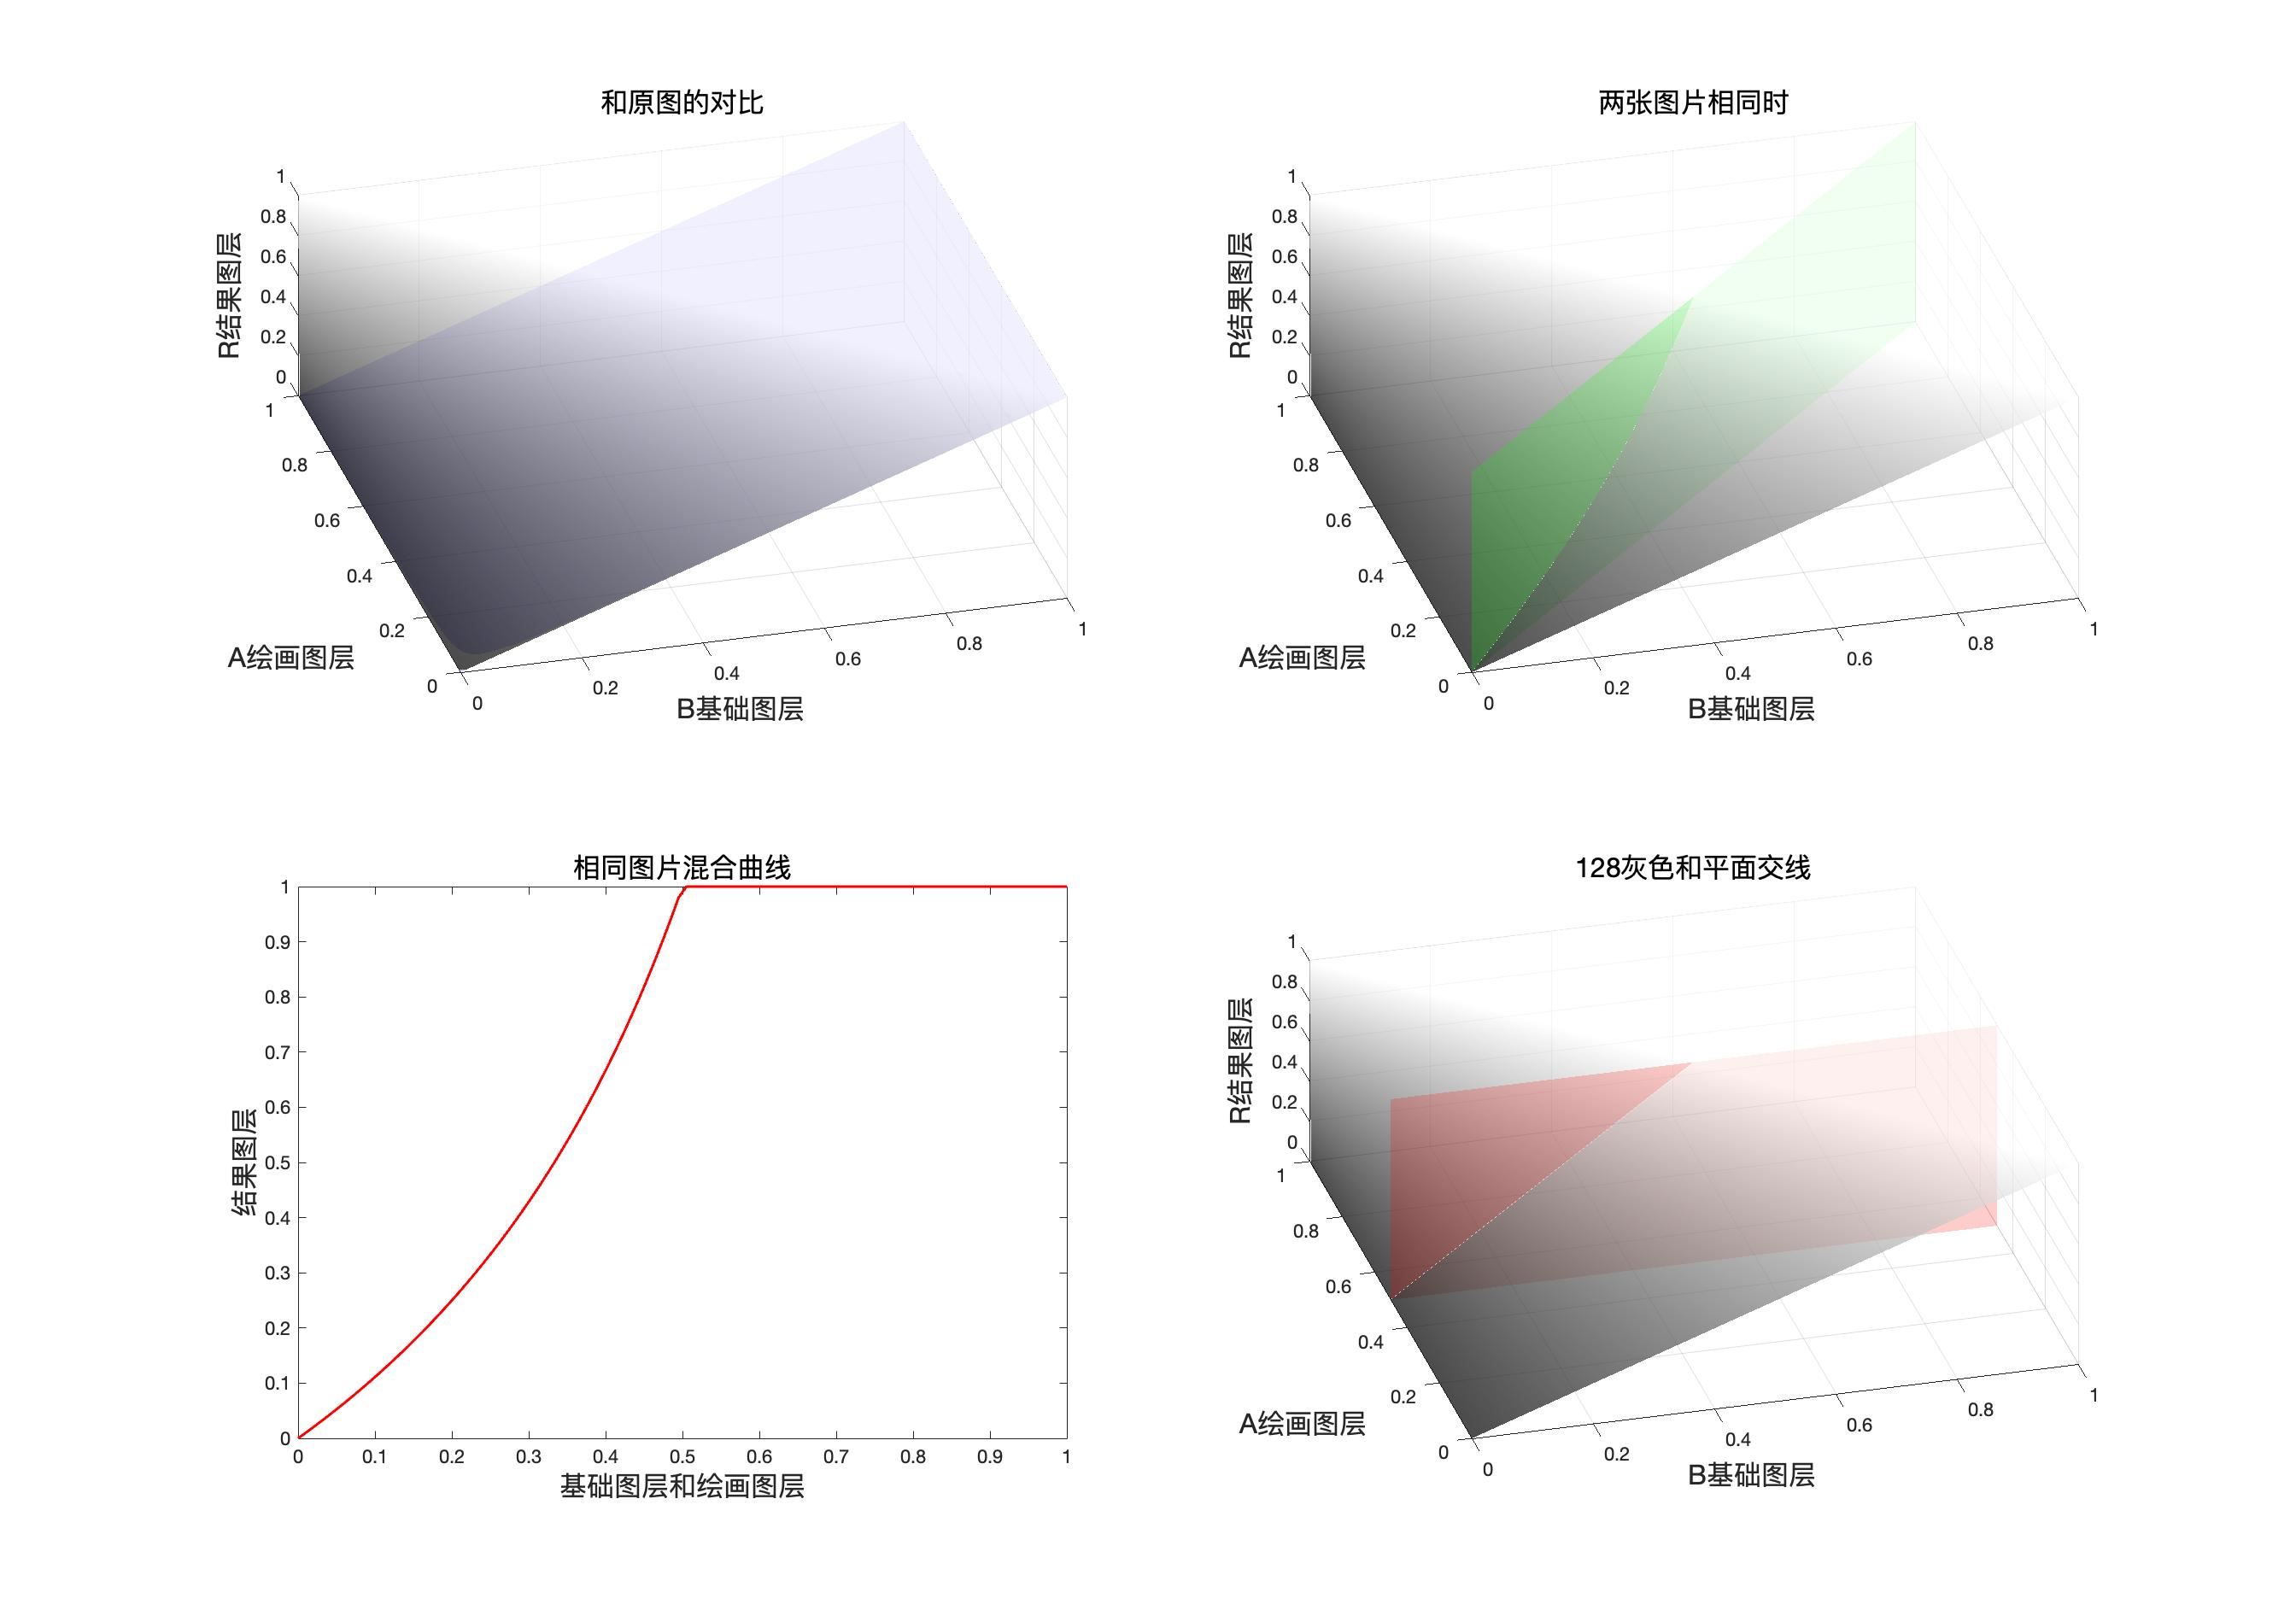
\includegraphics[width=\linewidth]{figure/颜色减淡.jpg}
	\caption{}
	\label{fig:}
\end{figure}

\newpage
\subsection{ 程序模拟该模式计算结果}

\begin{lstlisting}
	// 颜色减淡
	public static BlendColor ColorDodge(BlendColor colorBase, BlendColor colorBlend, double fill, double opacity) {
		double red = ColorDodgeChannel(colorBase.red.get01Value(), colorBlend.red.get01Value(), fill);
		double green = ColorDodgeChannel(colorBase.green.get01Value(), colorBlend.green.get01Value(), fill);
		double blue = ColorDodgeChannel(colorBase.blue.get01Value(), colorBlend.blue.get01Value(), fill);
		return ColorUtils.Opacity(colorBase, new BlendColor(red * 255, green * 255, blue * 255), opacity);
	}
	
	private static double ColorDodgeChannel(double base, double blend, double fill) {
		return ColorUtils.round((base) / ((1 - blend * fill)), 1, 0);
	}
	
\end{lstlisting}


\begin{result}
\item 颜色减淡(ColorDodge)    RGB[120.56,  85.92,  71.66]~ HSY[17.50,  48.89,  94.74 ]~ HSB[ 17.50,  40.56,  47.28]
\end{result}

\subsection{ 验证}
% TODO: \usepackage{graphicx} required
\begin{figure}[h!]
	\centering
	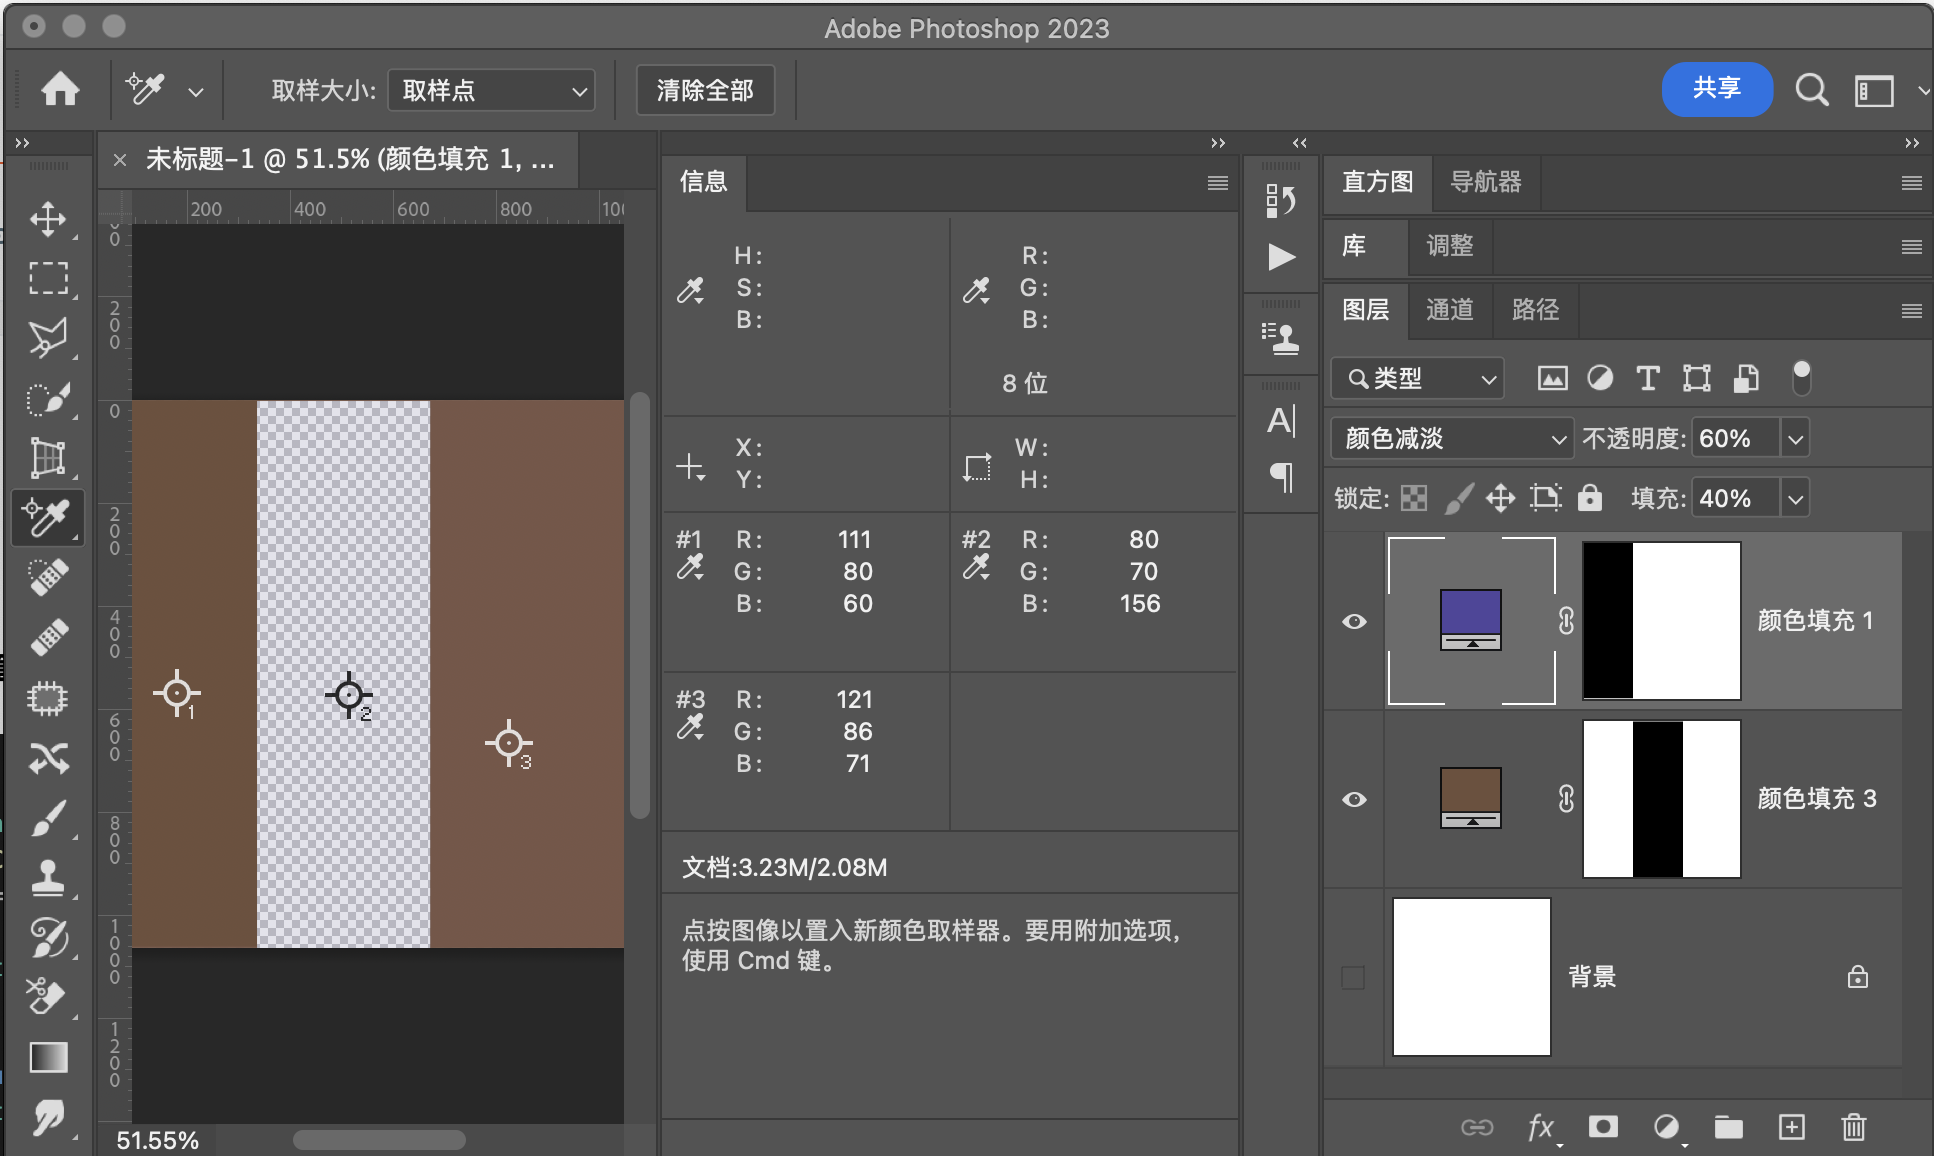
\includegraphics[width=\linewidth]{figure/colordodge}
	\caption{}
	\label{fig:colordodge}
\end{figure}


\subsection{ 用途示例}

1:组合成为亮光模式

2:制造光线,同时保护暗部细节

\newpage
\section{ 浅色Lighter}

浅色模式是深色模式的相反模式,可以通过深色三次负片操作得到
计算细节简单来说就是求和,比较大小,大的留下了,\text{若}求和的结果一样,就计算明度,明度大的留下了。

\subsection{ 公式}

	\begin{equation}
		\begin{aligned}
			Pix_r &=Lighter(Pix_b,Pix_a)\\&=\left\{\begin{aligned}&Pix_a && Sum(Pix_a)>Sum(Pix_b)\\&Pix_a&&  Sum(Pix_a)=Sum(Pix_b)\text{且}Lum(Pix_a)>Lum(Pix_b)\\&Pix_b&&  Sum(Pix_b)>Sum(Pix_a)\\&Pix_b&&  Sum(Pix_a)=Sum(Pix_b)\text{且}Lum(Pix_b)>Lum(Pix_a)\end{aligned}\right.
		\end{aligned}
	\end{equation}
	\begin{notice}
		\item 其中:\begin{flushleft}
			$Lum(Pix) = 0.3RC+0.59GC+0.11BC$\\
			$Sum(Pix) = RC+GC+BC$
		\end{flushleft}
		
	\end{notice}
	

\subsection{ 融合填充}


\begin{equation}
	r=Fill(Pix_b,Pix_a) =fill\times Pix_r+(1-fill)\times Pix_b
	\end{equation}

\subsection{ 融合不透明度}


\begin{equation}
	r=Opacity(Pix_b,Pix_a)=op\times Fill(Pix_b,Pix_a)+(1-op)\times Pix_b
\end{equation}

\subsection{ 三次负片操作相互转换}
\begin{equation}\begin{aligned}
		Pix_r &=1-Darker(1-Pix_b,1-Pix_a)\\&=\left\{\begin{aligned}&1-(1-Pix_a) && Sum(1-Pix_a)<Sum(1-Pix_b)\\&1-(1-Pix_b)&&  Sum(1-Pix_a)>Sum(1-Pix_b)\\&1-(1-Pix_b)&&  Sum(1-Pix_a)=Sum(1-Pix_b)\text{且}Lum(1-Pix_b)<Lum(1-Pix_a)\\&1-(1-Pix_a)&&  Sum(1-Pix_a)=Sum(1-Pix_b)\text{且}Lum(1-Pix_b)>Lum(1-Pix_a)\end{aligned}\right.\\&=\left\{\begin{aligned}&Pix_a&& Sum(Pix_a)>Sum(Pix_b)\\&Pix_b&&  Sum(Pix_a)<Sum(Pix_b)\\&Pix_b&&  Sum(Pix_a)=Sum(Pix_b)\text{且}Lum(Pix_b)>Lum(Pix_a)\\&Pix_a&&  Sum(Pix_a)=Sum(Pix_b)\text{且}Lum(Pix_b)<Lum(Pix_a)\end{aligned}\right.\\&=Lighter(Pix_b,Pix_a)
\end{aligned}\end{equation}


\subsection{ 程序模拟该模式计算结果}

\begin{lstlisting}
	// 浅色
	public static BlendColor Lighter(BlendColor colorBase, BlendColor colorBlend, double fill, double opacity) {
		double sumBase = colorBase.red.value + colorBase.green.value + colorBase.blue.value;
		double sumBlend = (colorBlend.red.value + colorBlend.green.value + colorBlend.blue.value);
		if (sumBase == sumBlend) {
			if (colorBase.getLum() > colorBlend.getLum()) {
				double red = colorBase.red.get01Value();
				double green = colorBase.green.get01Value();
				double blue = colorBase.blue.get01Value();
				return ColorUtils.Opacity(colorBase, new BlendColor(red * 255, green * 255, blue * 255), opacity);
			} else {
				double red = colorBase.red.get01Value() * (1 - fill) + colorBlend.red.get01Value() * fill;
				double green = colorBase.green.get01Value() * (1 - fill) + colorBlend.green.get01Value() * fill;
				double blue = colorBase.blue.get01Value() * (1 - fill) + colorBlend.blue.get01Value() * fill;
				return ColorUtils.Opacity(colorBase, new BlendColor(red * 255, green * 255, blue * 255), opacity);
			}
		}
		if (sumBase > sumBlend) {
			double red = colorBase.red.get01Value();
			double green = colorBase.green.get01Value();
			double blue = colorBase.blue.get01Value();
			return ColorUtils.Opacity(colorBase, new BlendColor(red * 255, green * 255, blue * 255), opacity);
		}
		double red = colorBase.red.get01Value() * (1 - fill) + colorBlend.red.get01Value() * fill;
		double green = colorBase.green.get01Value() * (1 - fill) + colorBlend.green.get01Value() * fill;
		double blue = colorBase.blue.get01Value() * (1 - fill) + colorBlend.blue.get01Value() * fill;
		return ColorUtils.Opacity(colorBase, new BlendColor(red * 255, green * 255, blue * 255), opacity);
		
	}
\end{lstlisting}

\begin{result}
\item 浅    色(Lighter)       RGB[111.00,  80.00,  60.00]~ HSY[23.53,  51.00,  87.10 ]~ HSB[ 23.53,  45.95,  43.53]
\end{result}
\newpage
\subsection{ 验证}

% TODO: \usepackage{graphicx} required
\begin{figure}[h!]
	\centering
	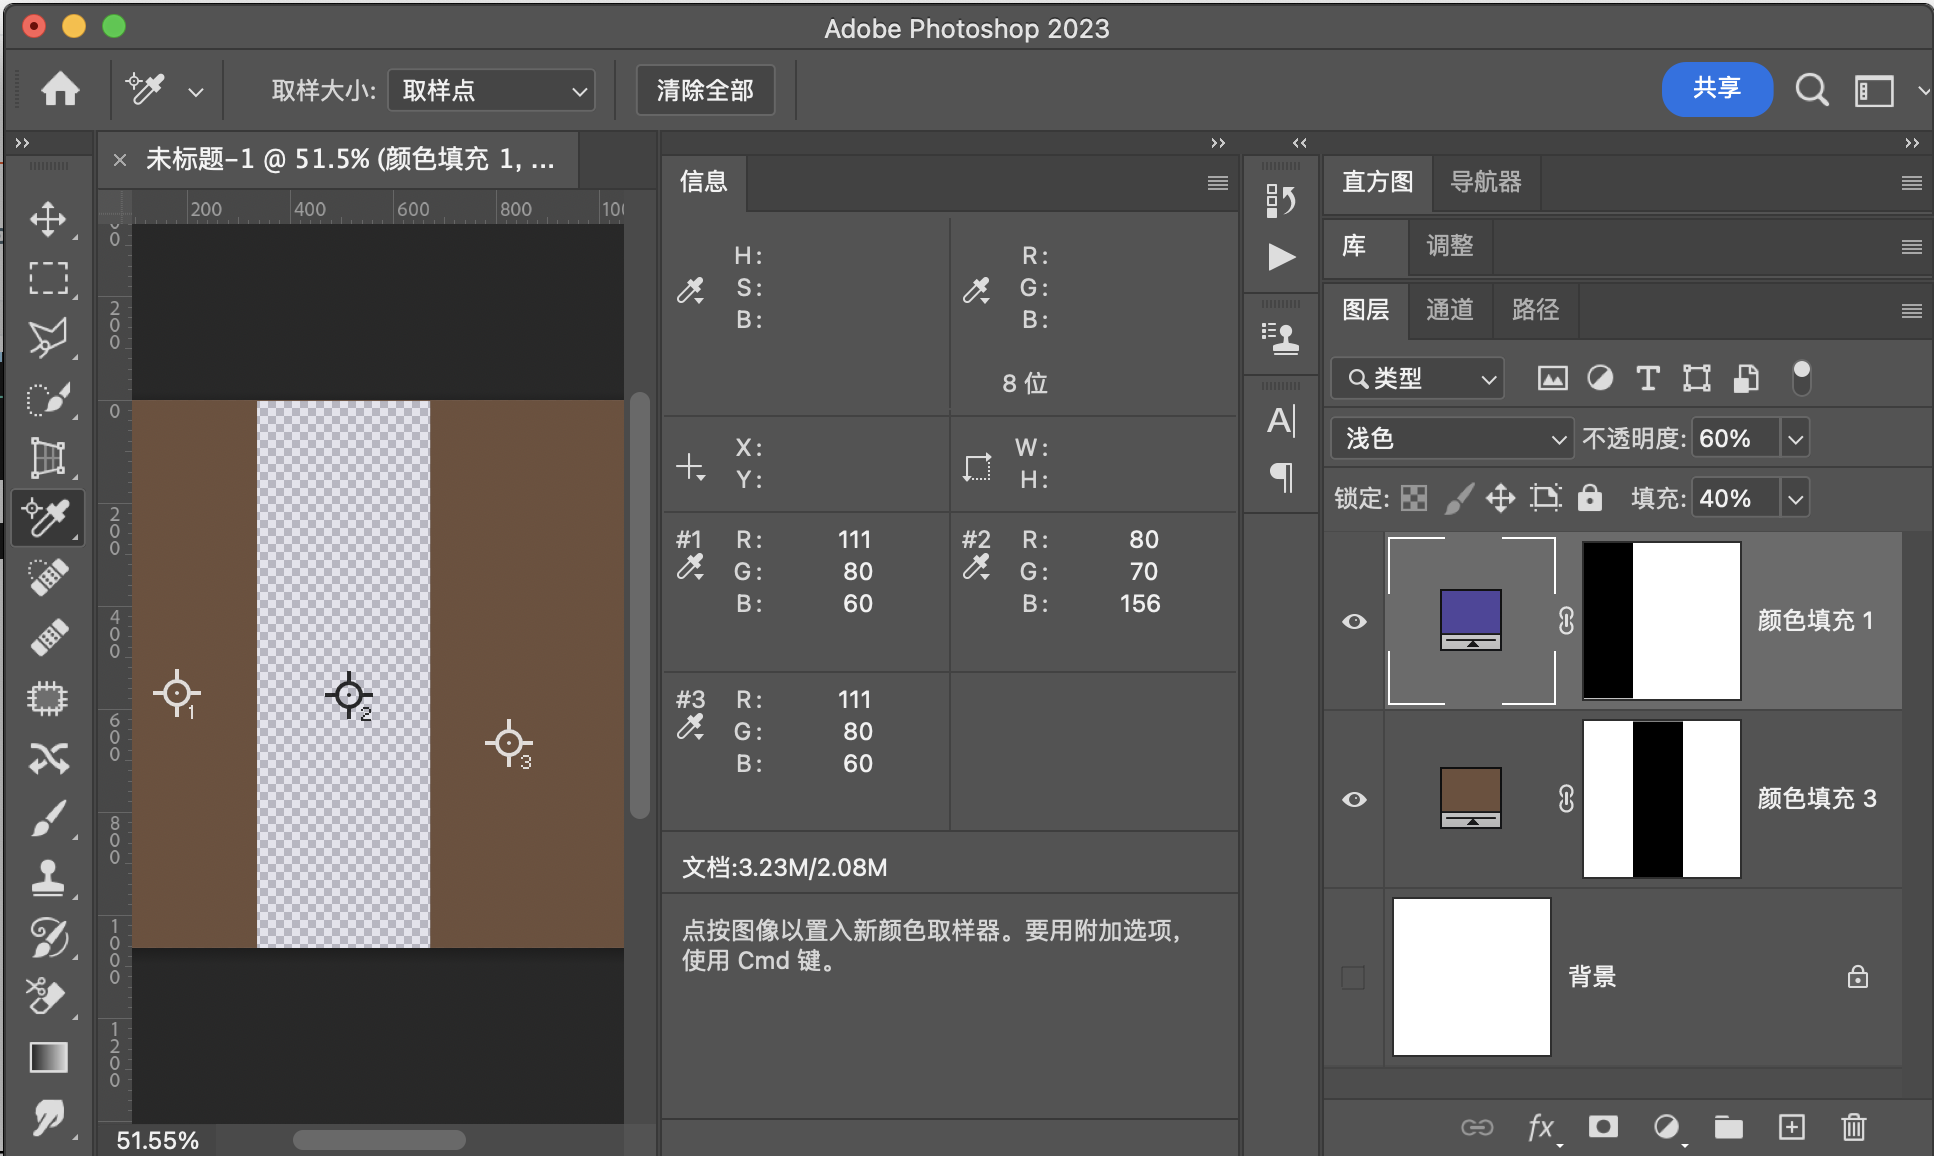
\includegraphics[width=\linewidth]{figure/lighter}
	\caption{}
	\label{fig:lighter}
\end{figure}
%
%\subsection{ 用途示例}
%
%保留像素中通道和较大的像素,可用于将背景较暗或相似但是部分不相同的图片融合。相当于做了一个复杂的通道蒙版,并且这个蒙版非常精确,精确到像素。



\chapter{对比度组}
\begin{introduction}
   \item 这一组都是相反的混合模式的组合,基本都是让暗的变暗,亮的变亮,所以这一组被称为对比度组,组合的分割界限是基础图层或者混合图层中性灰平面
\end{introduction}
\section{ 叠加Overlay}

此模式是正片叠底和滤色的组合,组合依据是底图的中性灰平面,如果在$[0,128]$则使用正片叠底,\text{若}是在$(128,255]$之间,则是实用滤色。

\subsection{ 公式}

\begin{equation}
	\begin{aligned}r&=OverLay(b,a)=\left\{\begin{aligned}Multiply(2b,a)&&当 0\leq b \leq 0.5\\Screen(2(b-0.5),a)&&当 0.5< b \leq 1\\\end{aligned}\right.=\left\{\begin{aligned}2ba&&当 0\leq b \leq 0.5\\1-2(1-b)(1-a)&&当 0.5< b \leq 1\\\end{aligned}\right.\end{aligned}
\end{equation}

和填充还有不透明度的关系,以及公式可以参考正片叠底和滤色

\subsection{ 映射面和同图等效曲线}
% TODO: \usepackage{graphicx} required
\begin{figure}[h!]
	\centering
	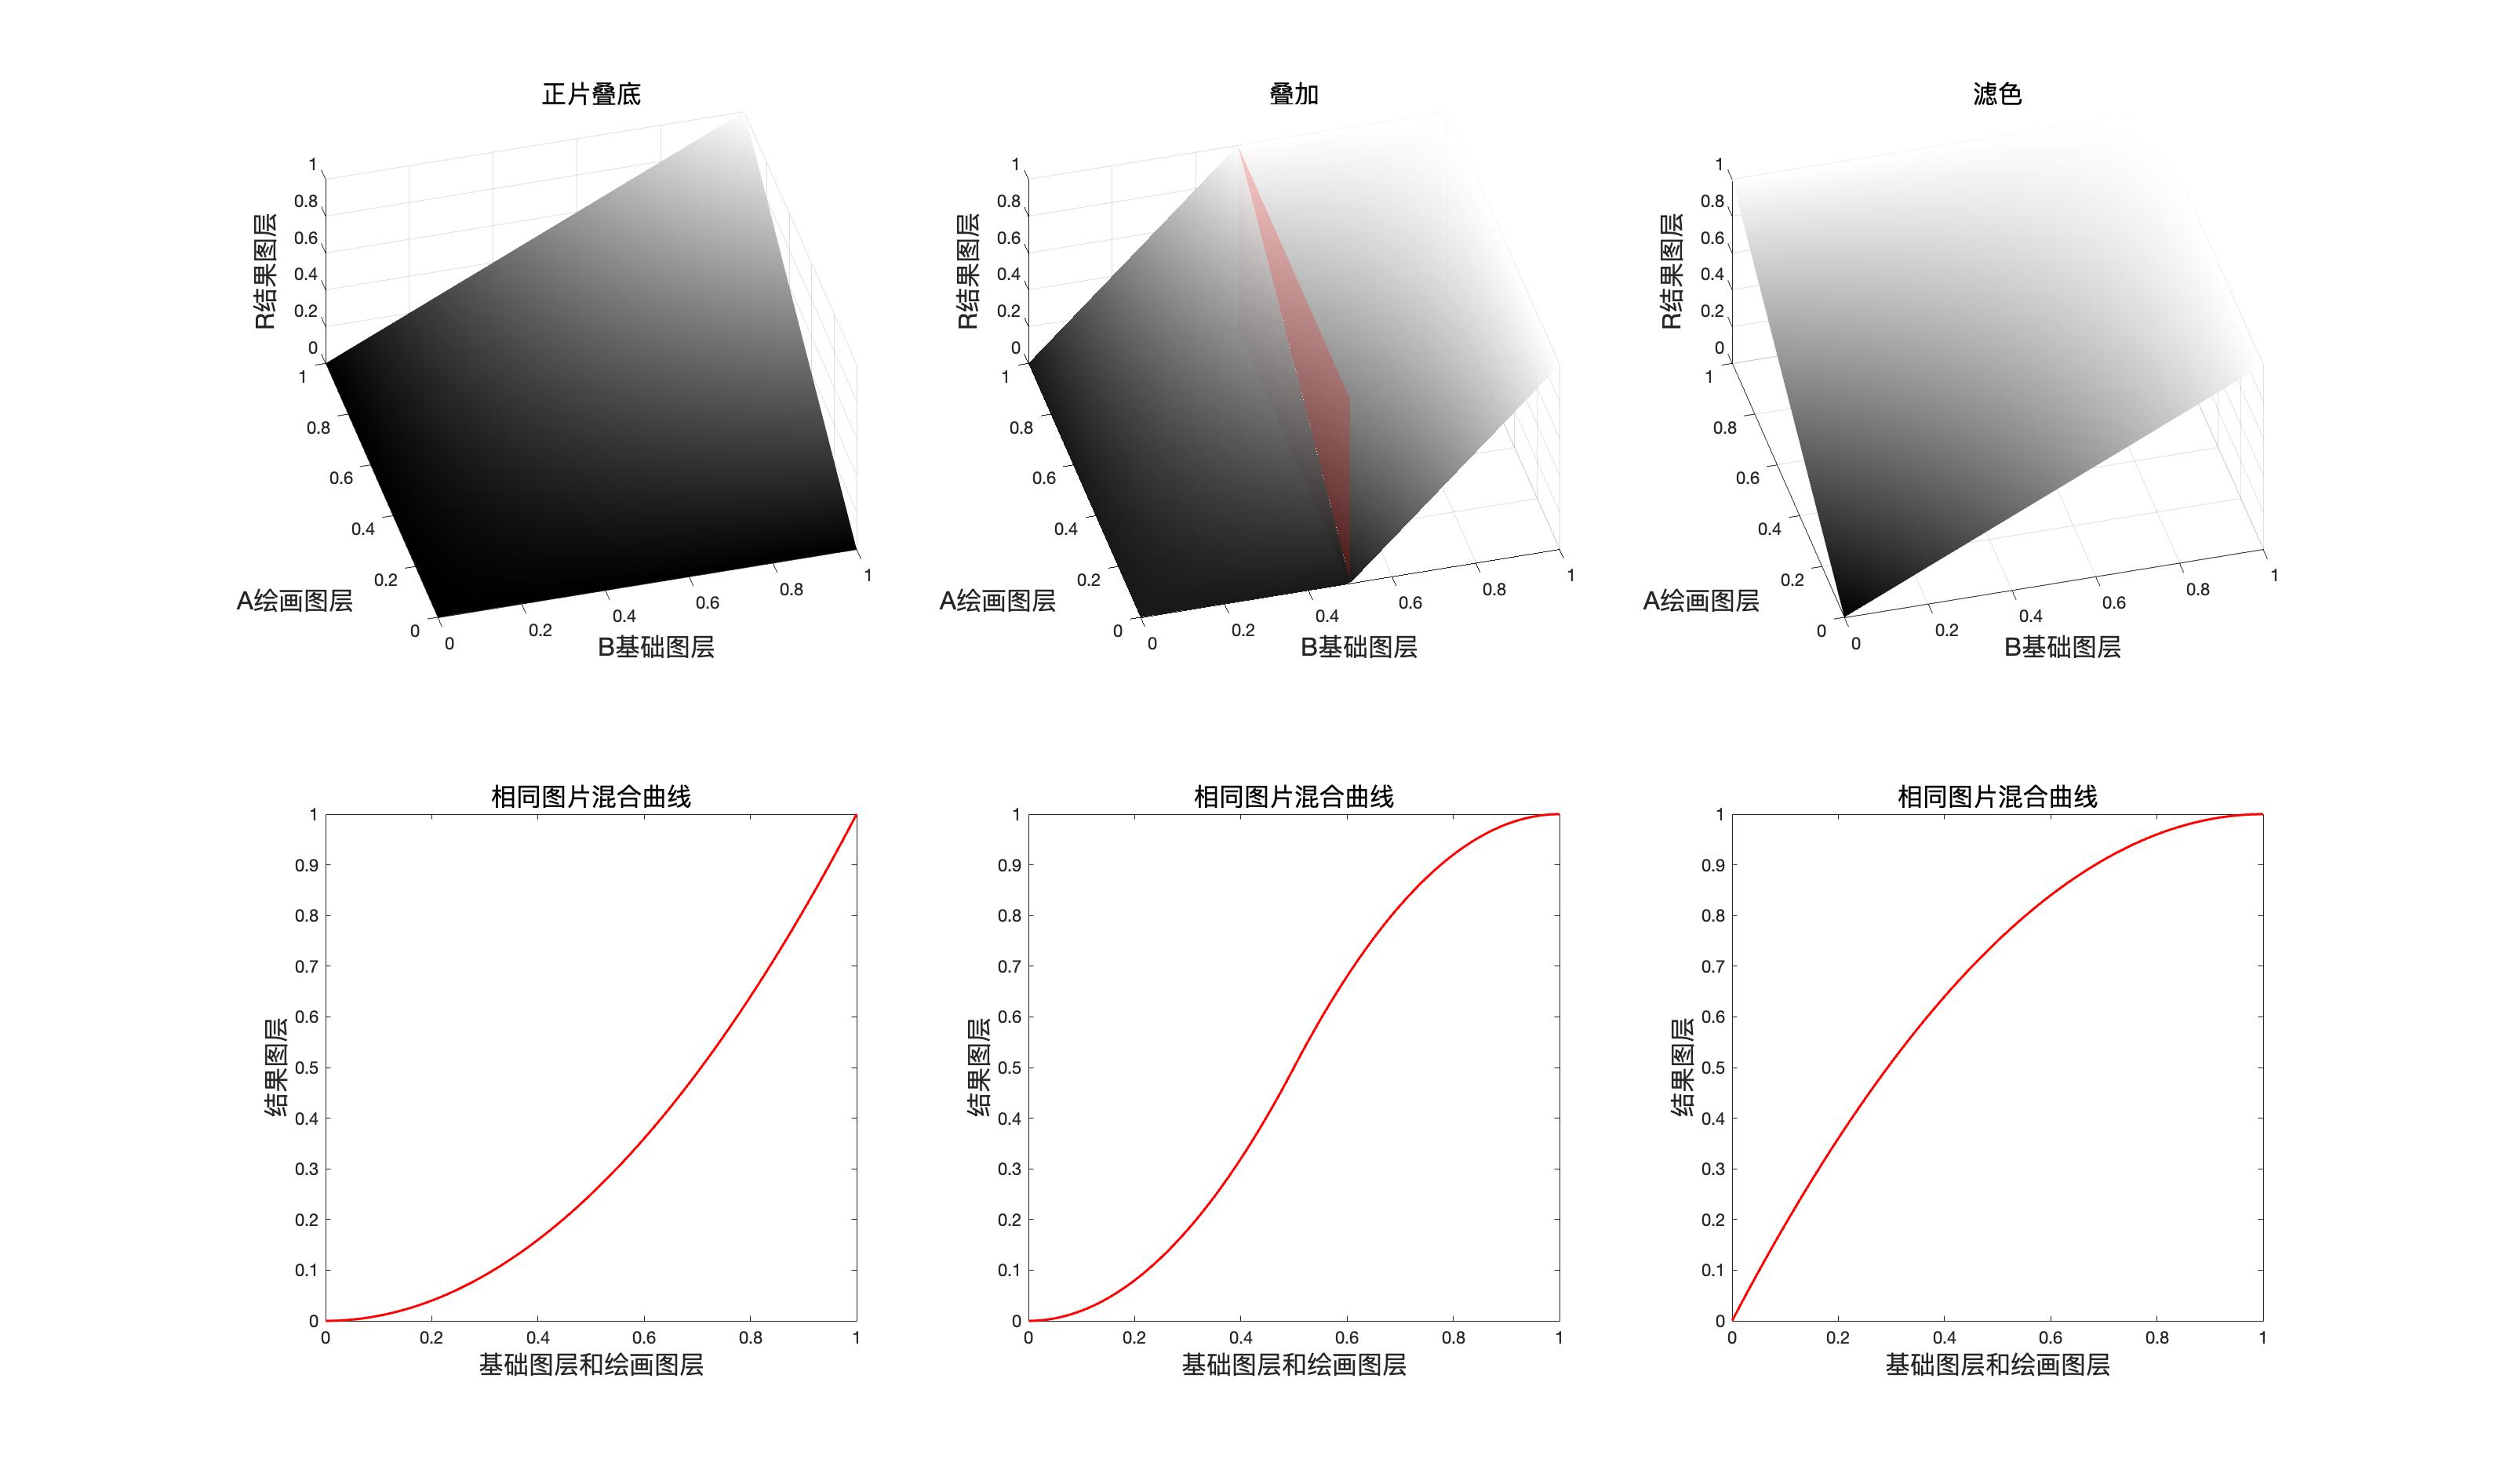
\includegraphics[width=\linewidth]{figure/叠加.jpg}
	\caption{}
	\label{fig:}
\end{figure}


\subsection{ 程序模拟该模式计算结果}

\begin{lstlisting}
	// 叠加
	public static BlendColor Overlay(BlendColor colorBase, BlendColor colorBlend, double fill, double opacity) {
		double red = OverlayChannel(colorBase.red.get01Value(), colorBlend.red.get01Value(), fill);
		double green = OverlayChannel(colorBase.green.get01Value(), colorBlend.green.get01Value(), fill);
		double blue = OverlayChannel(colorBase.blue.get01Value(), colorBlend.blue.get01Value(), fill);
		return ColorUtils.Opacity(colorBase, new BlendColor(red *255, green* 255, blue * 255), opacity);
	}
	
	private static double OverlayChannel(double baseValue, double blendValue, double fill) {
		if (baseValue <= 0.5) {
			return MulitplyChannel(baseValue, 2 * blendValue, fill);
		} else {
			return ScreenChannel(baseValue, 2 * (blendValue  - 0.5), fill);
		}
	}
\end{lstlisting}

\begin{result}
\item 叠    加(Overlay)       RGB[101.08,  71.34,  63.22]~ HSY[12.87,  37.86,  79.37 ]~ HSB[ 12.87,  37.45,  39.64]
\end{result}
\subsection{ 验证}
% TODO: \usepackage{graphicx} required
\begin{figure}[h!]
	\centering
	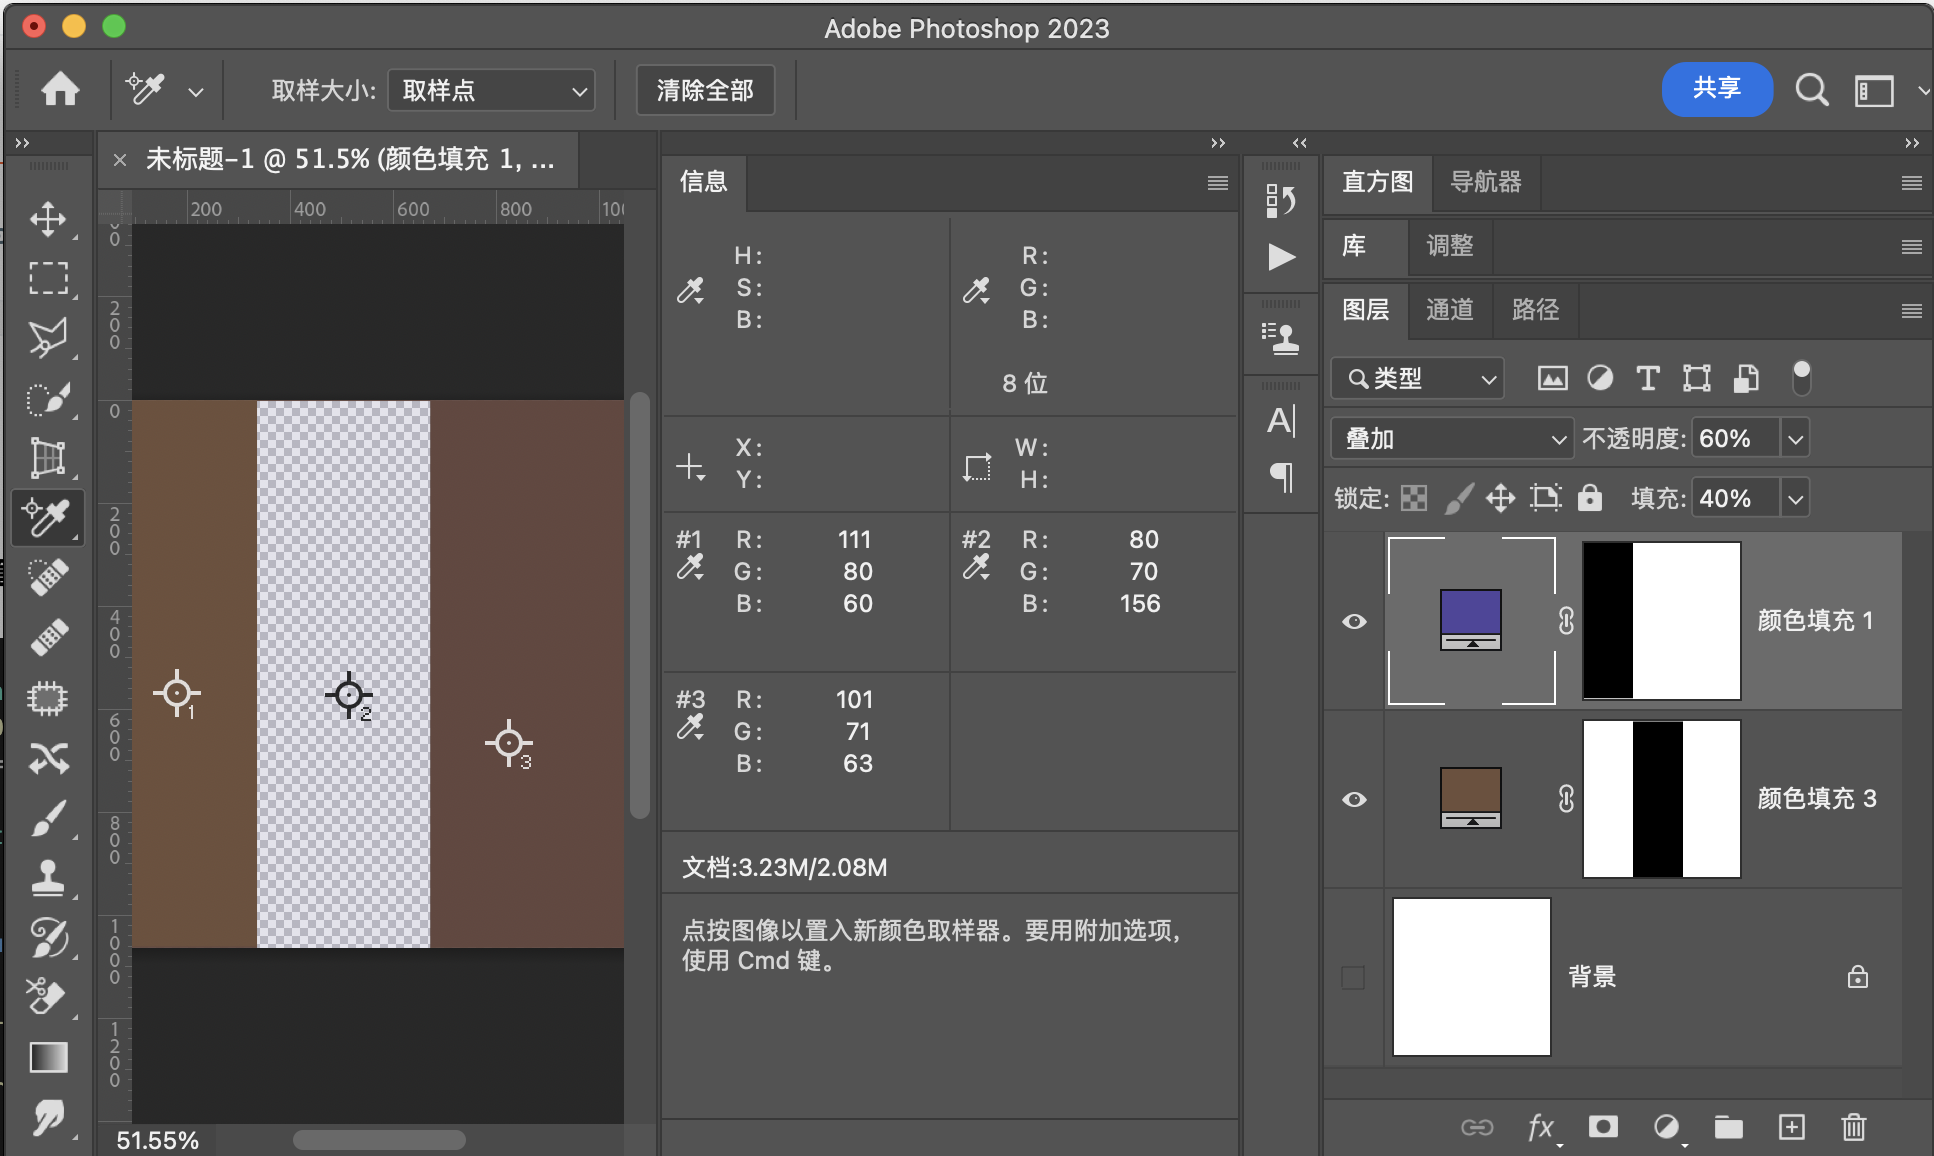
\includegraphics[width=\linewidth]{figure/overlay}
	\caption{}
	\label{fig:overlay}
\end{figure}


\subsection{ 用途示例}

1:同图混合增加图片对比度

2:和中性灰混合,达到局部提亮或者压黑

\newpage
\section{ 柔光SoftLight}

柔光模式是最复杂的一种混合模式,也是最巧妙的一种混合模式,柔光模式的本质是伽马矫正(gama correction)。配合混合图层的像素点的通道数值,再对原图层使用伽马矫正,二者通过配合就可以得到柔光模式。
\section{伽马矫正}
	 如果我们想了解柔光模式,首先必须了解什么是伽马矫正,伽马矫正,简单来说就是,将原像素通道数值通过幂次方的方式进行修改,比如平方和根号,例如我们由一个归一化之后为0.5的通道数值,我们对其进行系数为2的伽马矫正,则结果是$0.5^{\frac{1}{2}}=\sqrt{0.5}$,如果进行系数为$\frac{1}{2}$的伽马矫正,则结果为$0.5^2$

伽马矫正的数学表达式$output = input^{\frac{1}{gama}}$

其中$input$代表输入信号,$output$代表输出,$gama$代表伽马系数

系数为$2$的伽马矫正$output= input^{\frac{1}{2}}$	

系数为$\frac{1}{2}$的伽马矫正$output= input^{2}$

\subsection{ 公式}

% TODO: \usepackage{graphicx} required
\begin{figure}[h!]
	\centering
	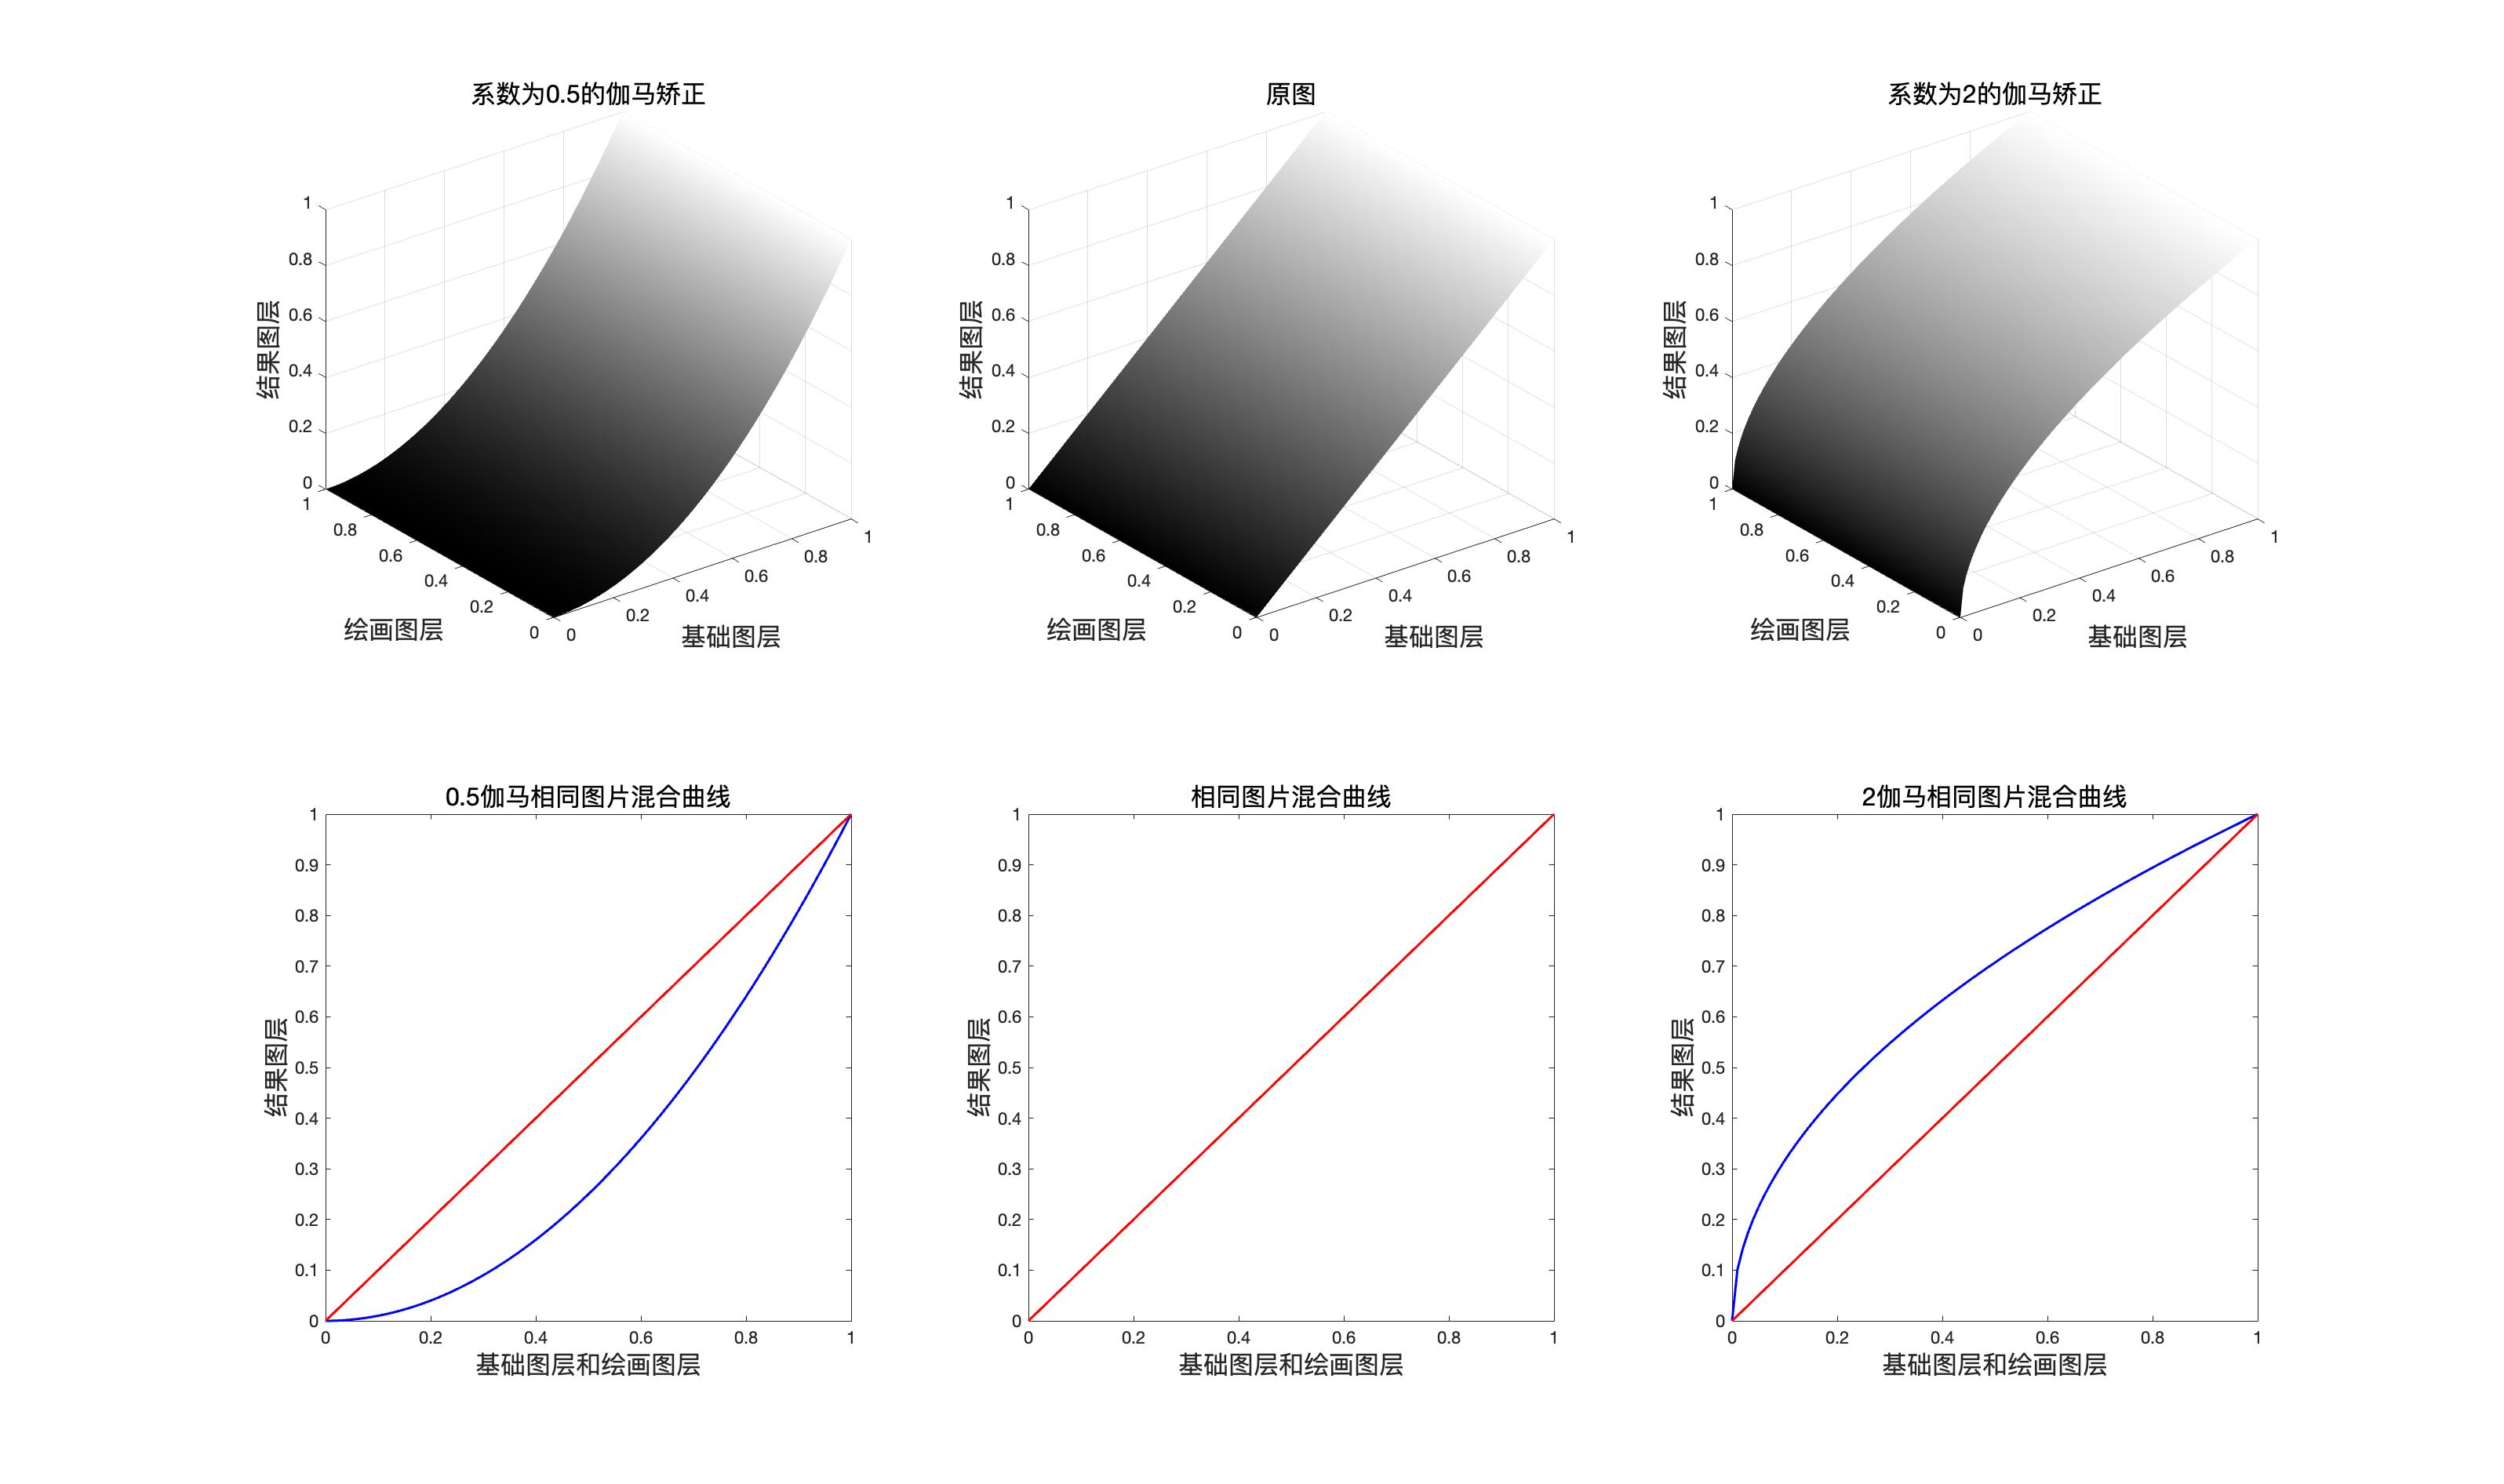
\includegraphics[width=\linewidth]{figure/伽马1}
	\caption{}
	\label{fig:1}
\end{figure}

于是对于系数为$\dfrac{1}{2}$的伽马矫正,稍微变换一下表达式

\begin{equation}
	r =b^2= (b-b^2) +b
	\end{equation}

然后再使用$(2a-1)$作为系数乘以差值项

\begin{equation}
	r = (2a-1)(b-b^2) +b
	\end{equation}
% TODO: \usepackage{graphicx} required
\begin{figure}[h!]
	\centering
	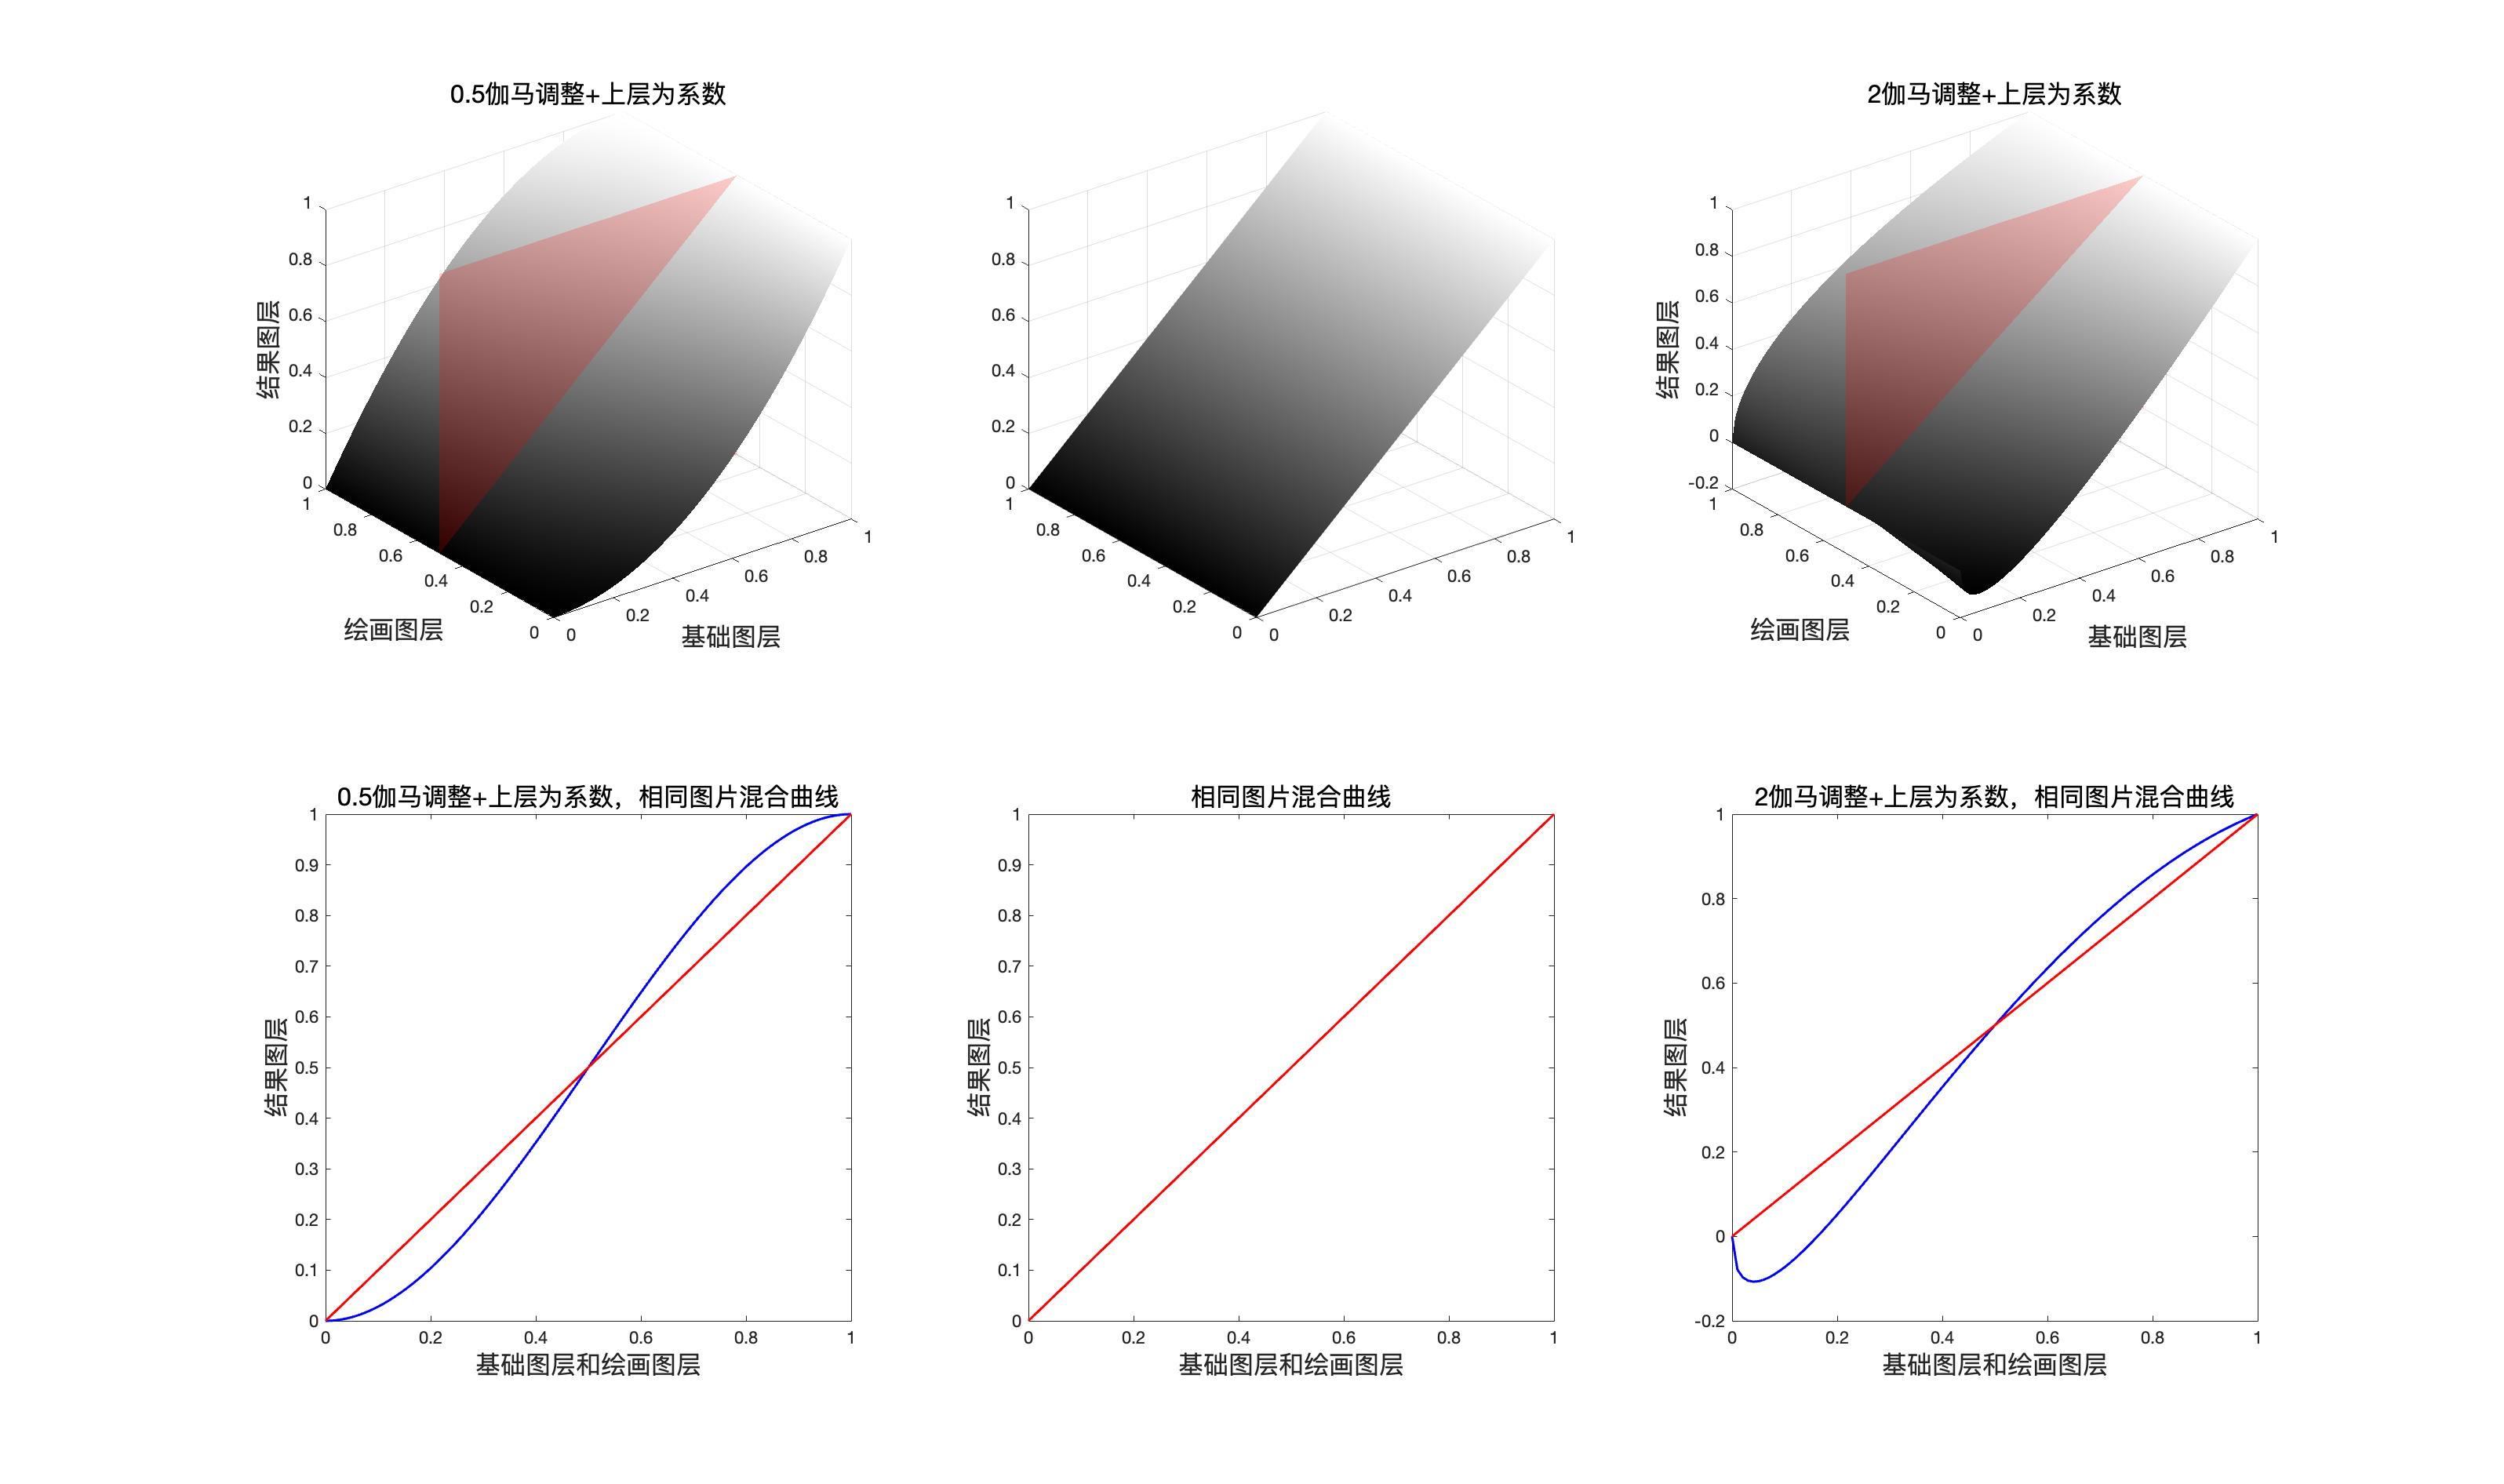
\includegraphics[width=\linewidth]{figure/伽马2}
	\caption{}
	\label{fig:2}
\end{figure}

于是对于系数为$2$的伽马矫正,稍微变换一下表达式

\begin{equation}
	r =\sqrt{b}= (\sqrt{b}-b) +b
	\end{equation}

然后再使用$(2a-1)$作为系数乘以差值项

\begin{equation}
	r =(2a-1)(\sqrt{b}-b) +b
\end{equation}

再将结果合并,我们就可以得到柔光模式的表达式。

\begin{equation}
	\begin{aligned}r&= SoftLight(b,a)=\left\{\begin{aligned}&(2a-1)(b^2-b)+b&a\leq0.5\\&(2a-1)(\sqrt{b}-b)+b&a>0.5\end{aligned}\right.\end{aligned}
\end{equation}


\begin{notice}
	\item 如果使用一句话概括柔光模式的数学表达式,就是“以混合图层为系数的系数为$\frac{1}{2}$和$2$的伽马矫正”
	\item  在 PS中伽马矫正可以在色阶工具和曝光度工具中找到
\end{notice}
 \newpage
\subsection{ 映射面和同图等效曲线}
% TODO: \usepackage{graphicx} required
\begin{figure}[h!]
	\centering
	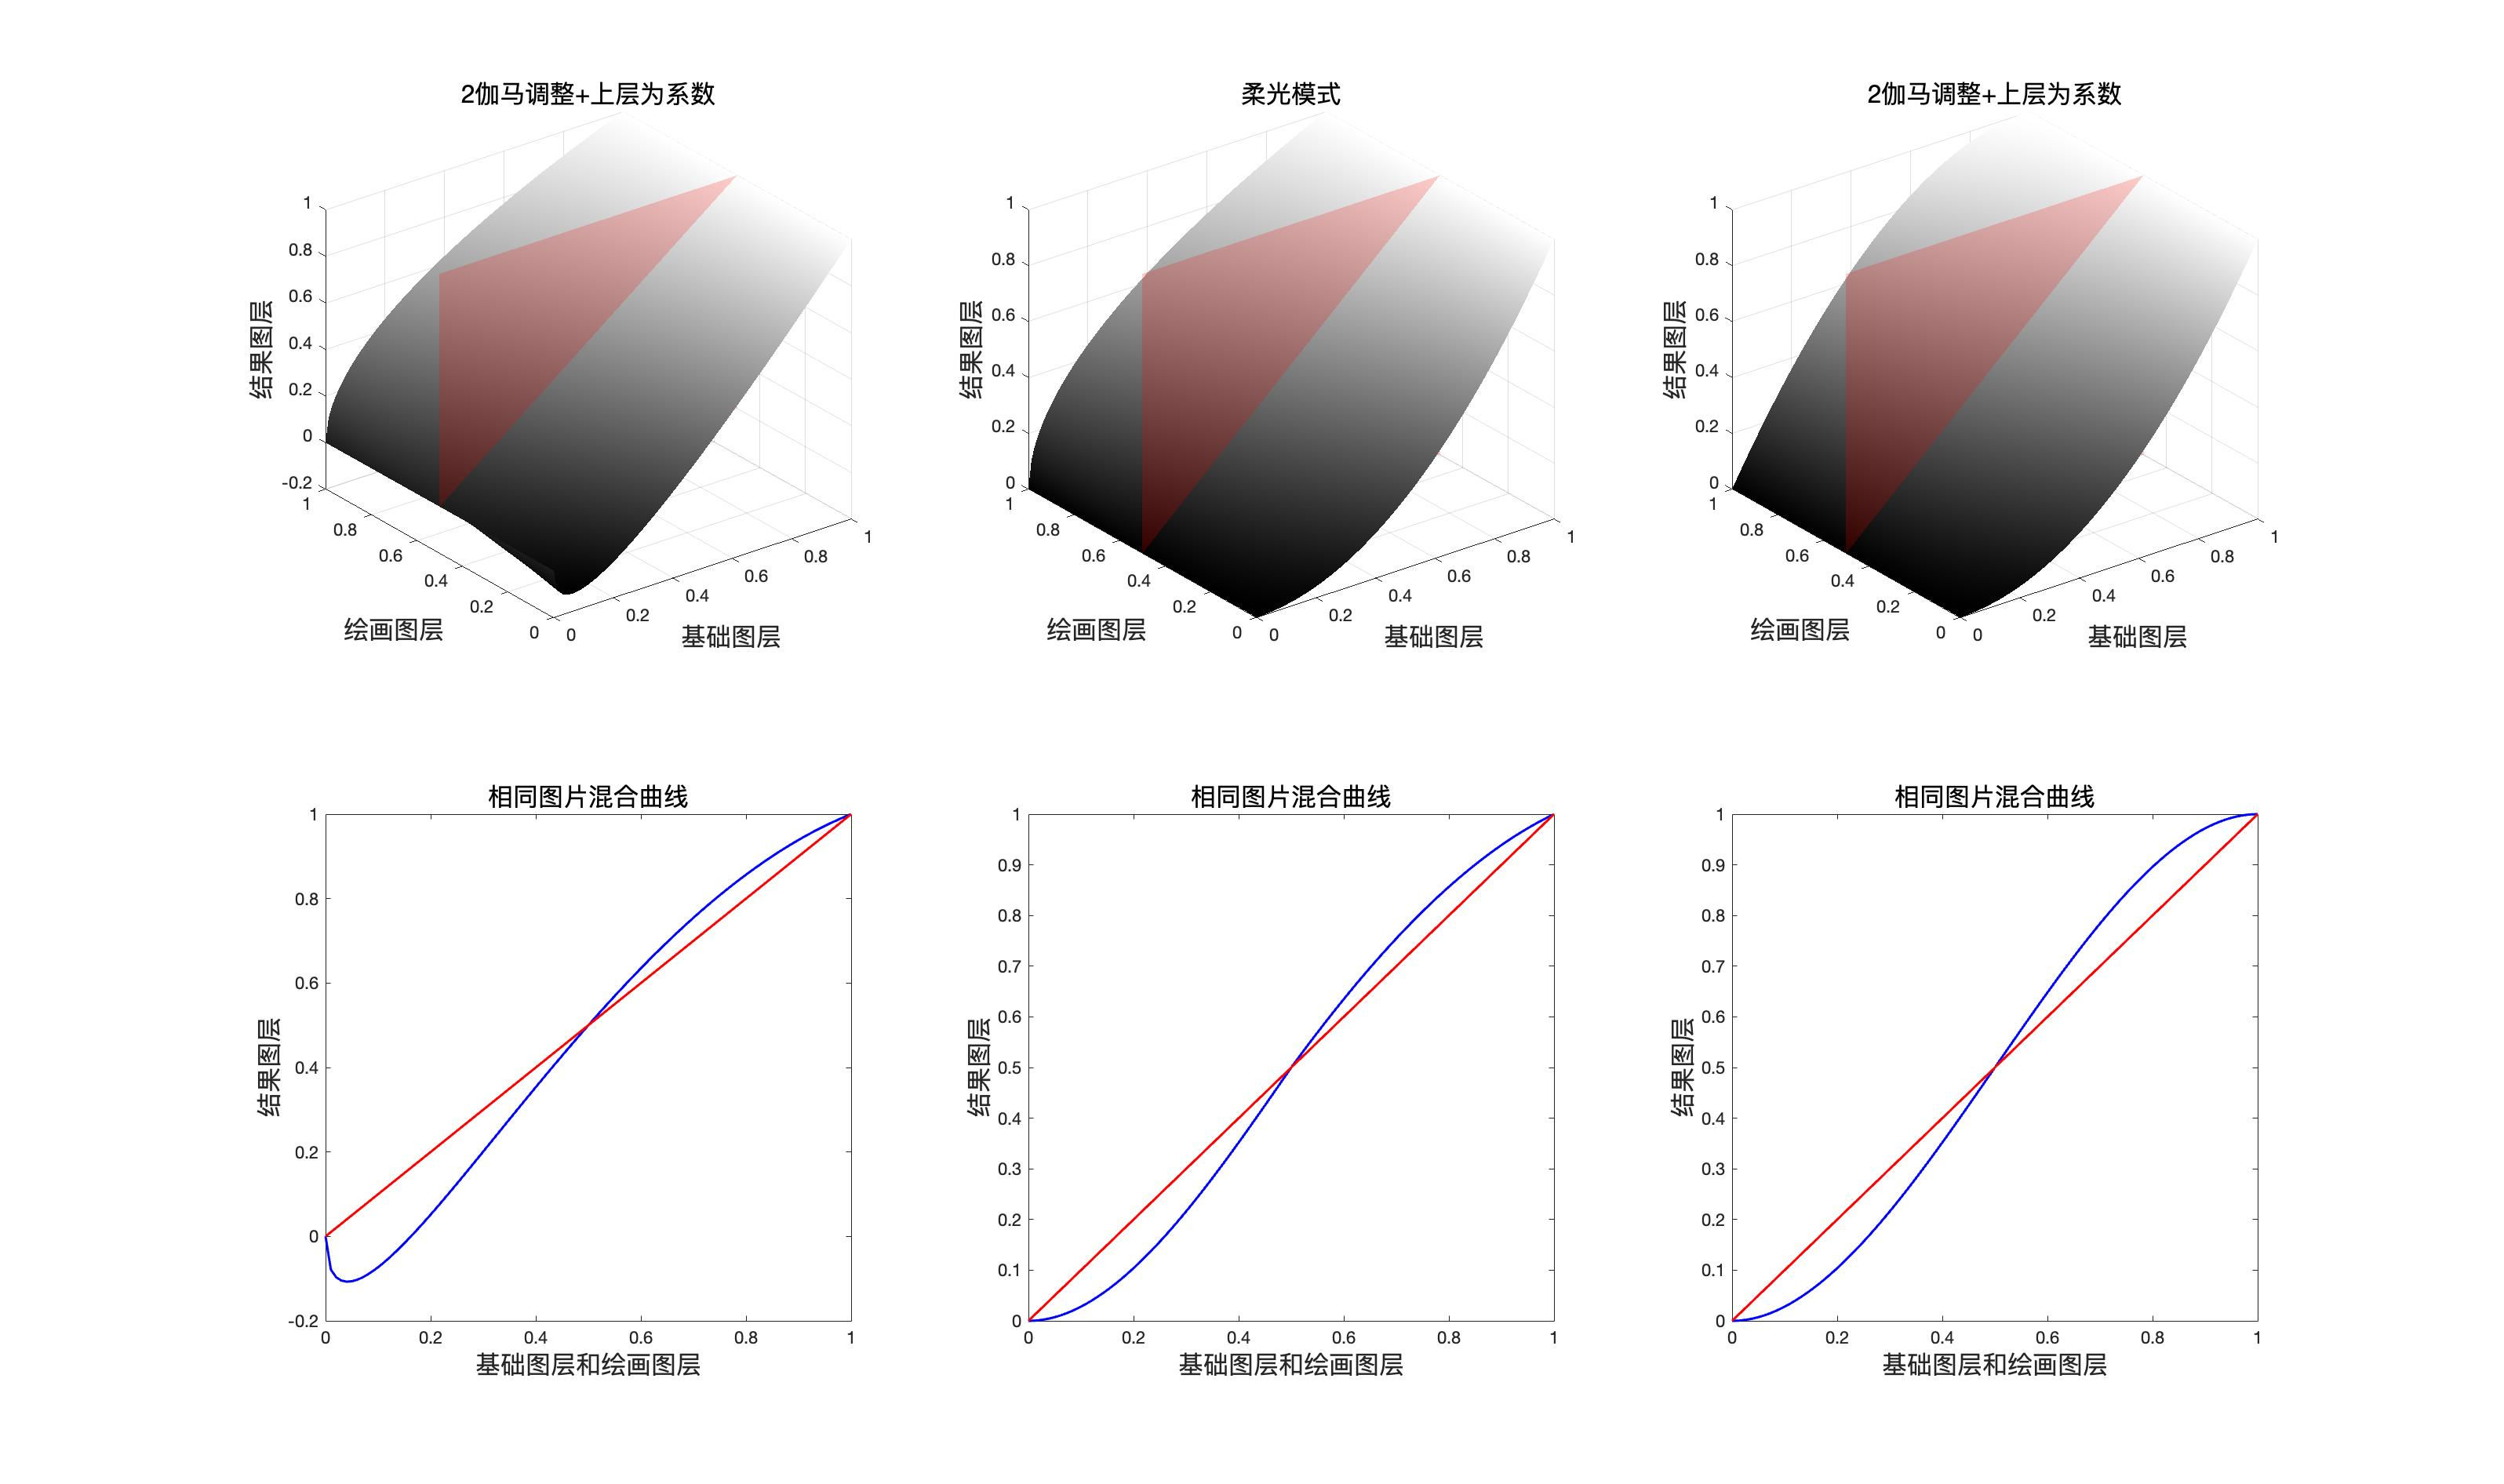
\includegraphics[width=\linewidth]{figure/柔光}
	\caption{}
	\label{fig:}
\end{figure}


\subsection{ 程序模拟该模式计算结果}

\begin{lstlisting}
	// 柔光
	public static BlendColor SoftLight(BlendColor colorBase, BlendColor colorBlend, double fill, double opacity) {
		double red = SoftLightChannel(colorBase.red.get01Value(), colorBlend.red.get01Value(), fill);
		double green = SoftLightChannel(colorBase.green.get01Value(), colorBlend.green.get01Value(), fill);
		double blue = SoftLightChannel(colorBase.blue.get01Value(), colorBlend.blue.get01Value(), fill);
		return ColorUtils.Opacity(colorBase, new BlendColor(red * 255, green * 255, blue * 255), opacity);
	}
	
	private static double SoftLightChannel(double baseValue, double blendValue, double fill) {
		if (blendValue <= 0.5) {
			return (baseValue + (2 * blendValue - 1) * (baseValue  -baseValue * baseValue)) * fill
			+ (1 - fill) * baseValue;
		} else {
			return (baseValue + (2 * blendValue - 1) * (SoftLightChannelsub(baseValue)  - baseValue)) * fill
			+ (1 - fill) * baseValue;
		}
	}
	
	private static double SoftLightChannelsub(double value) {
		if (value <= 0.25) {
			return ((16 * value  - 12) * value + 4) * value;
		} else {
			return Math.sqrt(value);
		}
	}
\end{lstlisting}



\begin{result}
\item 柔    光(SoftLight)     RGB[105.40,  74.06,  63.42]~ HSY[15.21,  41.98,  82.29 ]~ HSB[ 15.21,  39.83,  41.33]
\end{result}

\subsection{ 验证}
% TODO: \usepackage{graphicx} required
\begin{figure}[h!]
	\centering
	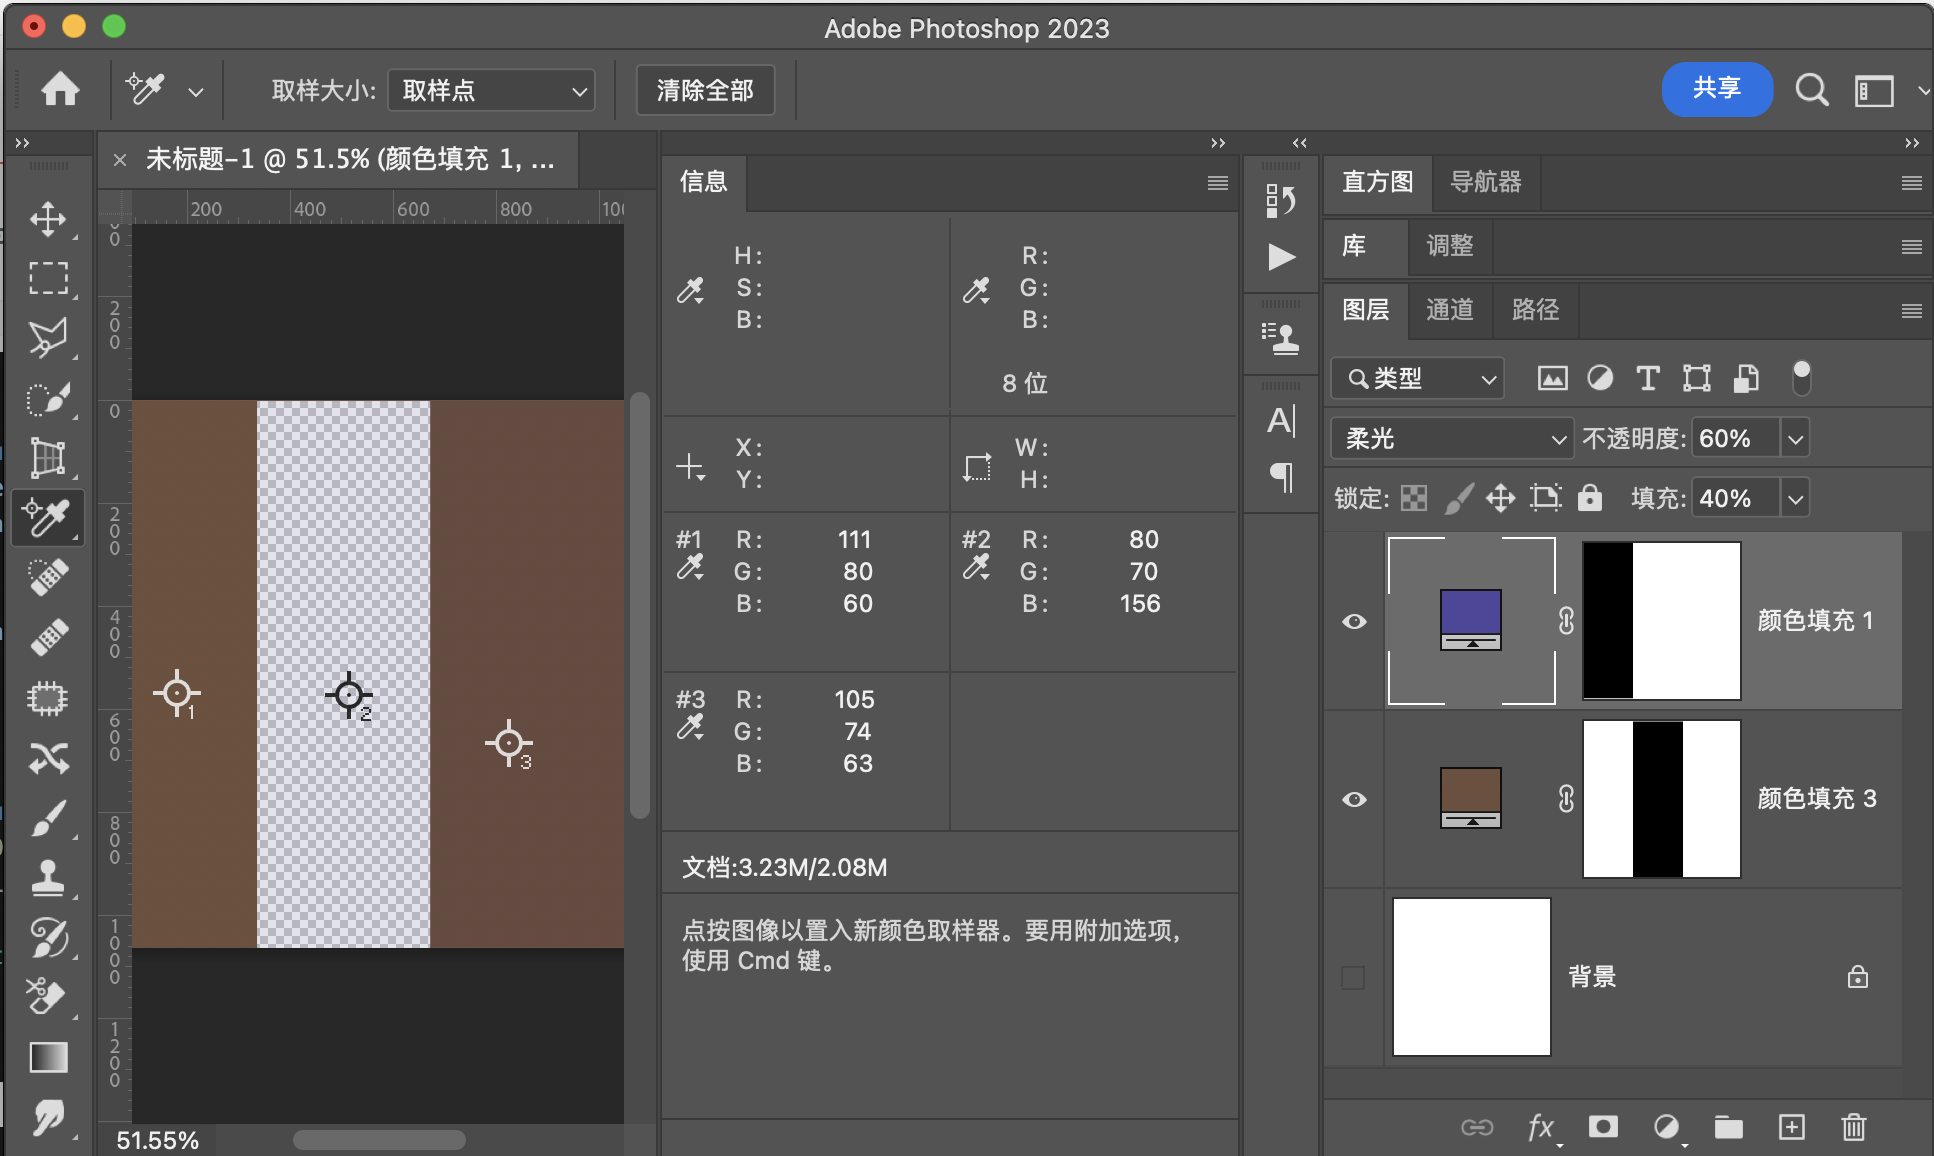
\includegraphics[width=\linewidth]{figure/softlight}
	\caption{}
	\label{fig:softlight}
\end{figure}


%
%\subsection{ 用途示例}
%
%1:同图混合增加图片对比度
%
%2:配合中性灰平面,实现局部提亮和压暗(dodge and burn)

\newpage
\section{ 强光HardLight}

此模式也是正片叠底和滤色的组合,组合的分割界限是混合图层中性灰平面,并且它和叠加模式是互逆的关系,也就是说,如果在强光模式下把基础图层和混合图层顺序调换,可以的到原顺序下叠加模式的效果。

\subsection{ 公式}

\begin{equation}
	\begin{aligned}r&= HardLight(b,a)=\left\{\begin{aligned}Multiply(b,2a)&&当 0\leq a \leq 0.5\\Screen(b,2(a-0.5))&&当 0.5< a \leq 1\\\end{aligned}\right.\\\\&=\left\{\begin{aligned}2ba&&当 0\leq a \leq 0.5\\1-2(1-b)(1-a)&&当 0.5< a \leq 1\\\end{aligned}\right.\end{aligned}
	\end{equation}

\subsection{ 和填充结合}

\begin{equation}
	\begin{aligned}r&= Fill(b,a)=\left\{\begin{aligned}fill\times Multiply(b,2a)+(1-fill)\times b&&当 0\leq a \leq 0.5\\fill\times Screen(b,2(a-0.5)))+(1-fill)\times b&&当 0.5< a \leq 1\\\end{aligned}\right.\end{aligned}
\end{equation}

\subsection{ 融合不透明度}
\begin{equation}
	r=Opacity(b,a)=op\times Fill(b,a)+(1-op)\times b
\end{equation}
\newpage
\subsection{ 映射面和同图等效曲线}
% TODO: \usepackage{graphicx} required
\begin{figure}[h!]
	\centering
	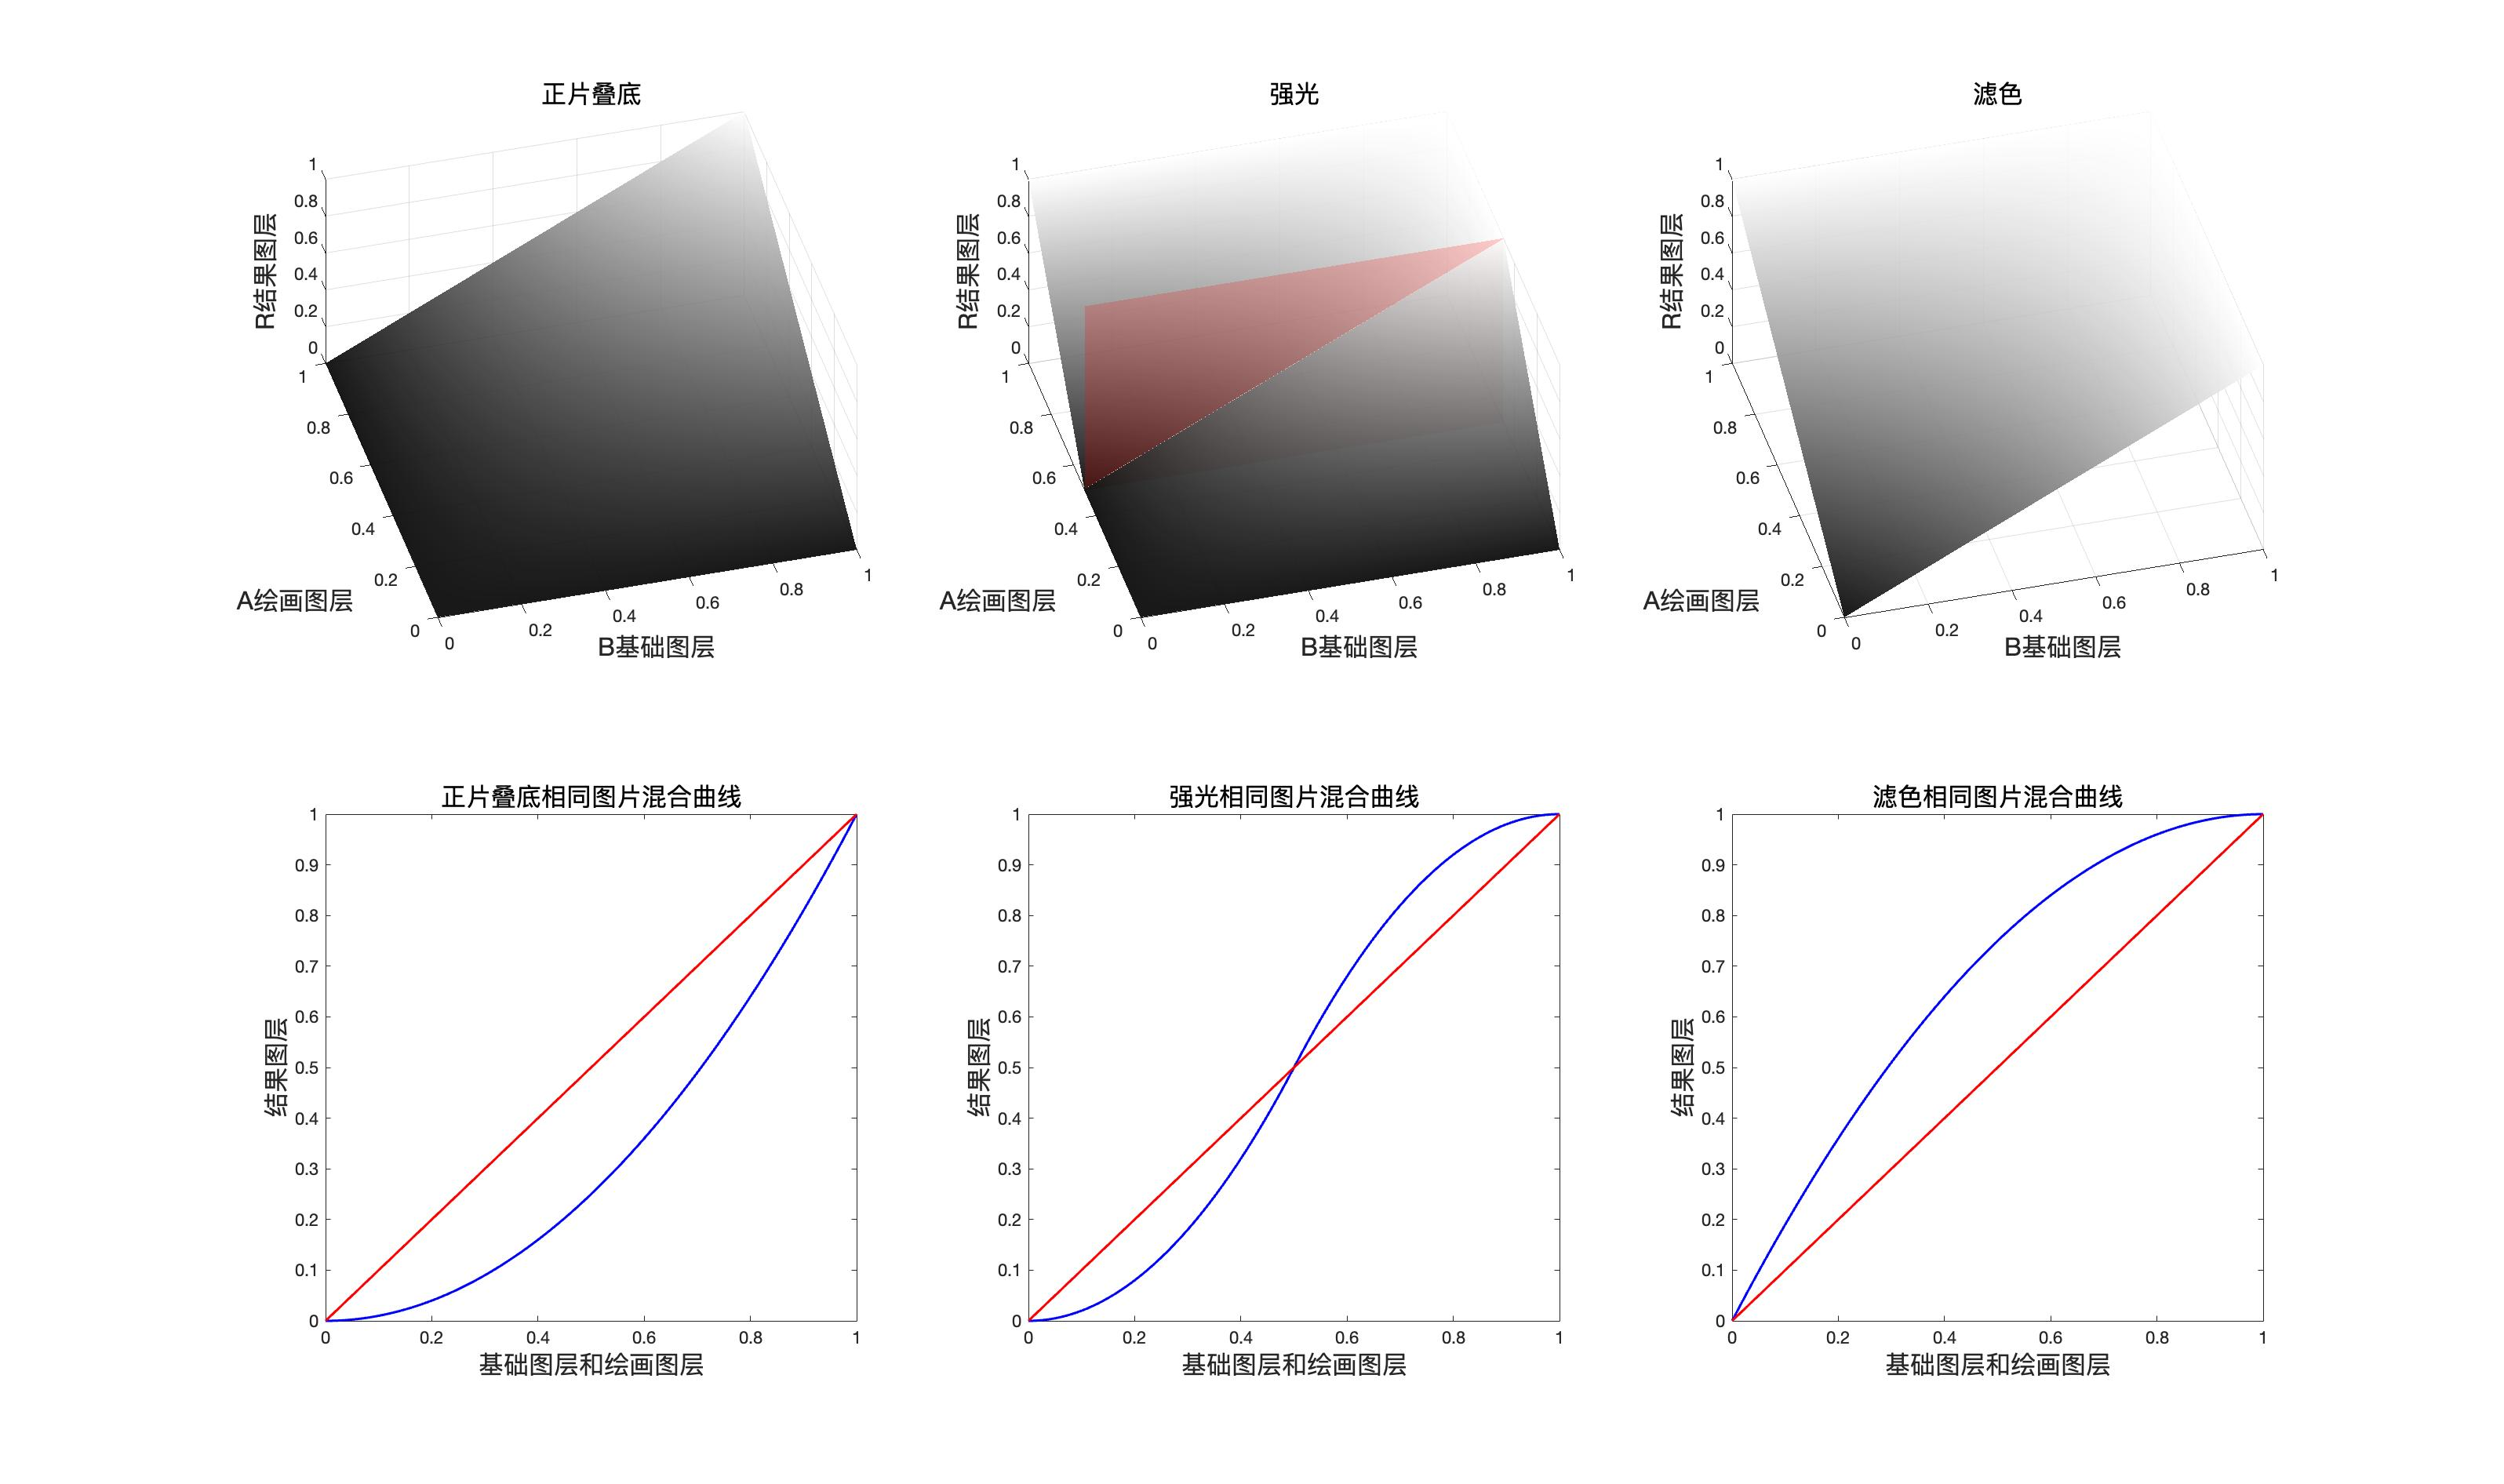
\includegraphics[width=\linewidth]{figure/强光}
	\caption{}
	\label{fig:}
\end{figure}



\subsection{ 程序模拟该模式计算结果}
\begin{lstlisting}
	// 强光
	public static BlendColor HardLight(BlendColor colorBase, BlendColor colorBlend, double fill, double opacity) {
		double red = HardLightChannel(colorBase.red.get01Value(), colorBlend.red.get01Value(), fill);
		double green = HardLightChannel(colorBase.green.get01Value(), colorBlend.green.get01Value(), fill);
		double blue = HardLightChannel(colorBase.blue.get01Value(), colorBlend.blue.get01Value(), fill);
		return ColorUtils.Opacity(colorBase, new BlendColor(red * 255, green * 255, blue * 255), opacity);
	}
	
	private static double HardLightChannel(double baseValue, double blendValue, double fill) {
		if (blendValue <= 0.5) {
			return MulitplyChannel(baseValue, 2 * blendValue, fill);
		} else {
			
			return ScreenChannel(baseValue, 2 * (blendValue  - 0.5), fill);
		}
	}
\end{lstlisting}

\begin{result}
\item 强    光(HardLight)     RGB[101.08,  71.34,  70.46]~ HSY[1.72,  30.61,  80.16  ]~ HSB[  1.72,  30.29,  39.64]
\end{result}
\subsection{ 验证}
% TODO: \usepackage{graphicx} required
\begin{figure}[h!]
	\centering
	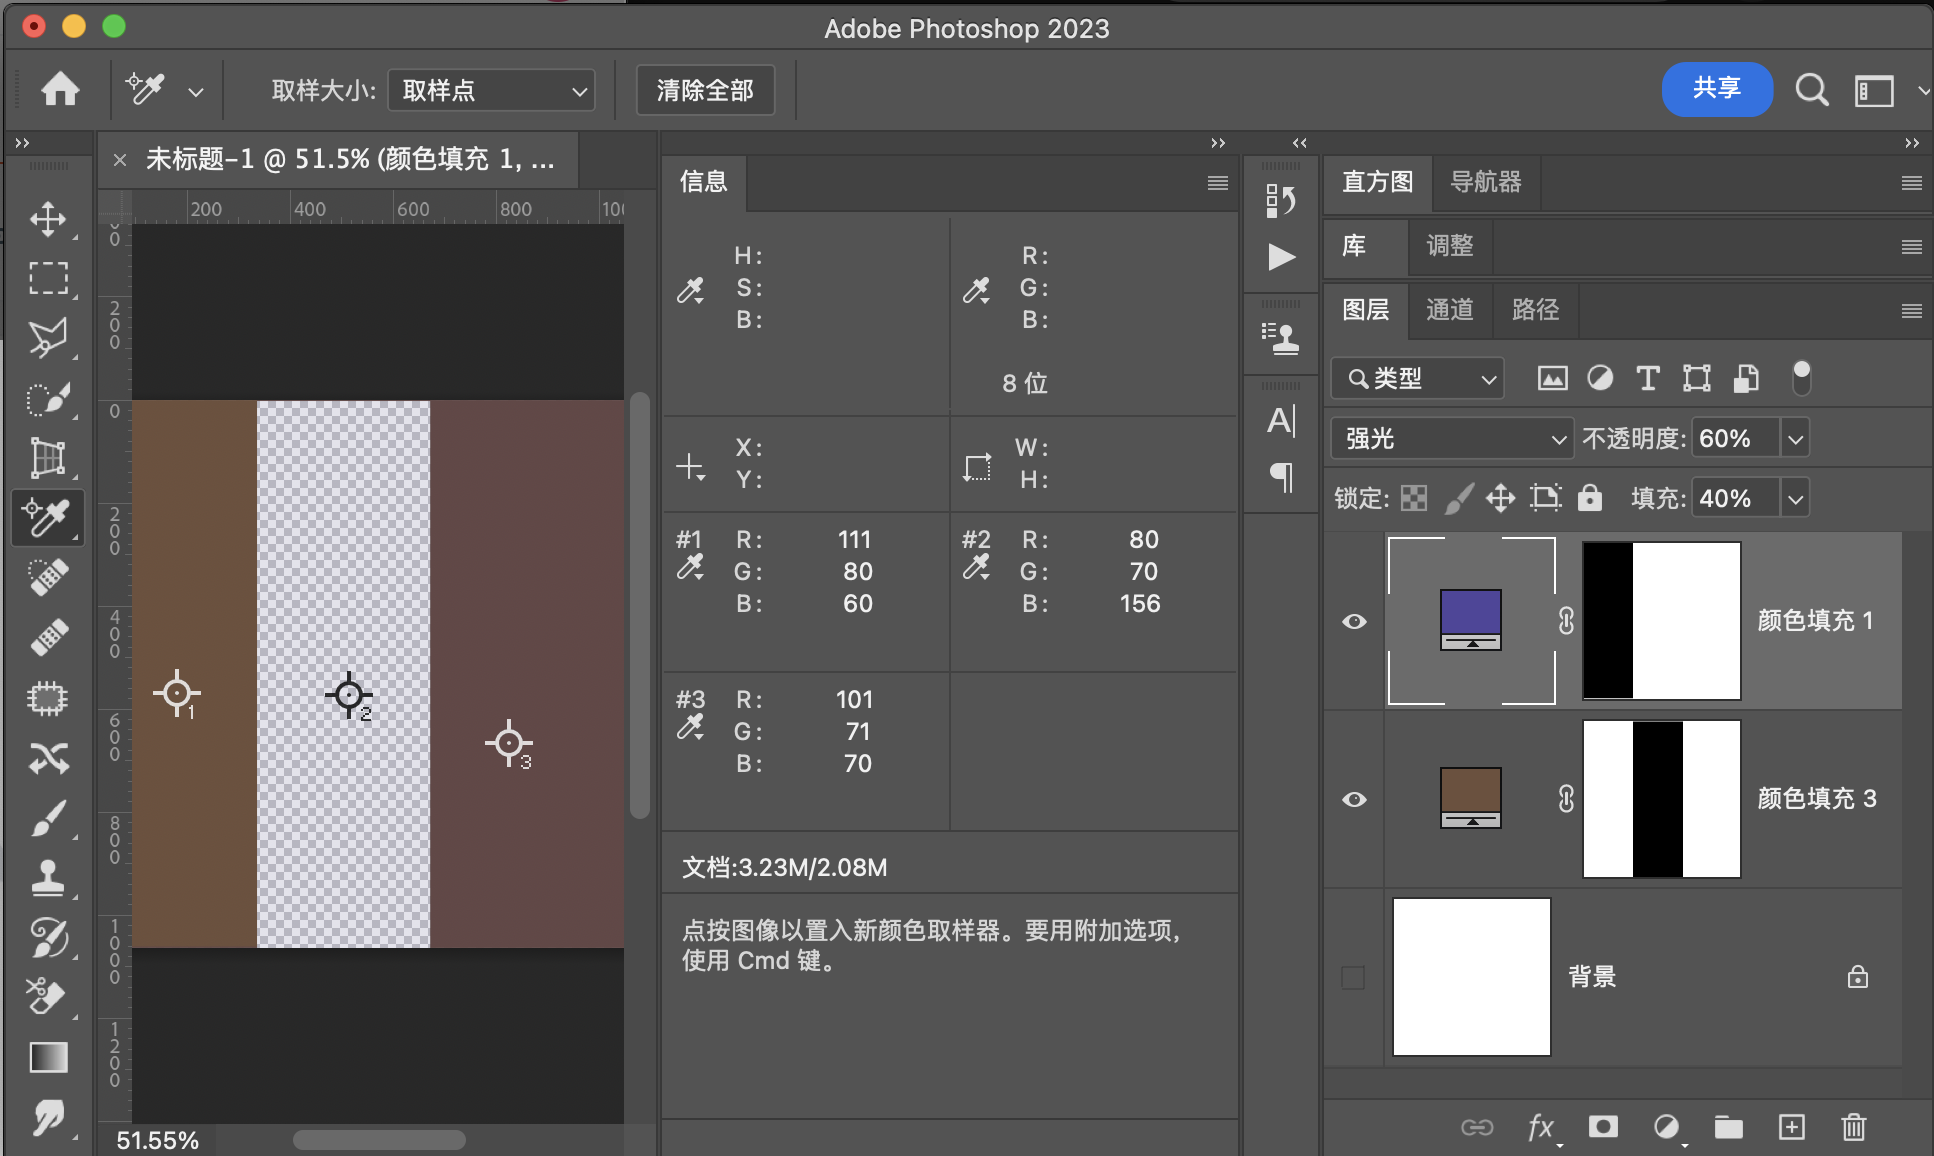
\includegraphics[width=\linewidth]{figure/hardlight}
	\caption{}
	\label{fig:hardlight}
\end{figure}


%\subsection{ 用途示例}
%
%1:同图混合增加图片对比度
%2:配合中性灰平面,实现dodge and burn.
\newpage
\section{ 线性光LinearLight}

线性光是线性减淡和线性加深的结合,组合的分割界限是混合图层中性灰平面,具体公式如下

\subsection{ 公式}

\begin{equation}
	\begin{aligned}r&= LinearLight(b,a)=\left\{\begin{aligned}LinearBurn(b,2a)&&当 0\leq a \leq 0.5\\LinearDodge(b,2(a-0.5))&&当 0.5< a \leq 1\\\end{aligned}\right.\\&=\left\{\begin{aligned}b+(2a)-1&&当 0\leq a \leq 0.5\\b+2(a-0.5)&&当 0.5< a \leq 1\\\end{aligned}\right.=b+2a-1\end{aligned}
	\end{equation}

\subsection{ 和填充结合}

\begin{equation}
	\begin{aligned}r&= Fill(b,a)=\left\{\begin{aligned}LinearBurn(b,2a\times fill)&&当 0\leq a \leq 0.5\\LinearDodge(b,2(a-0.5)\times fill)&&当 0.5< a \leq 1\\\end{aligned}\right.\\&=\left\{\begin{aligned}b+(2a)\times fill-1&&当 0\leq a \leq 0.5\\b+2(a-0.5)\times fill&&当 0.5< a \leq 1\\\end{aligned}\right.=\left\{\begin{aligned}b+2a\times fill-1&&当 0\leq a \leq 0.5\\b+2a\times fill-1\times fill&&当 0.5< a \leq 1\\\end{aligned}\right.\end{aligned}
	\end{equation}

\subsection{ 融合不透明度}
\begin{equation}
	r=Opacity(b,a)=op\times Fill(b,a)+(1-op)\times b
\end{equation}
\newpage
\subsection{ 映射面和同图等效曲线}
% TODO: \usepackage{graphicx} required
\begin{figure}[h!]
	\centering
	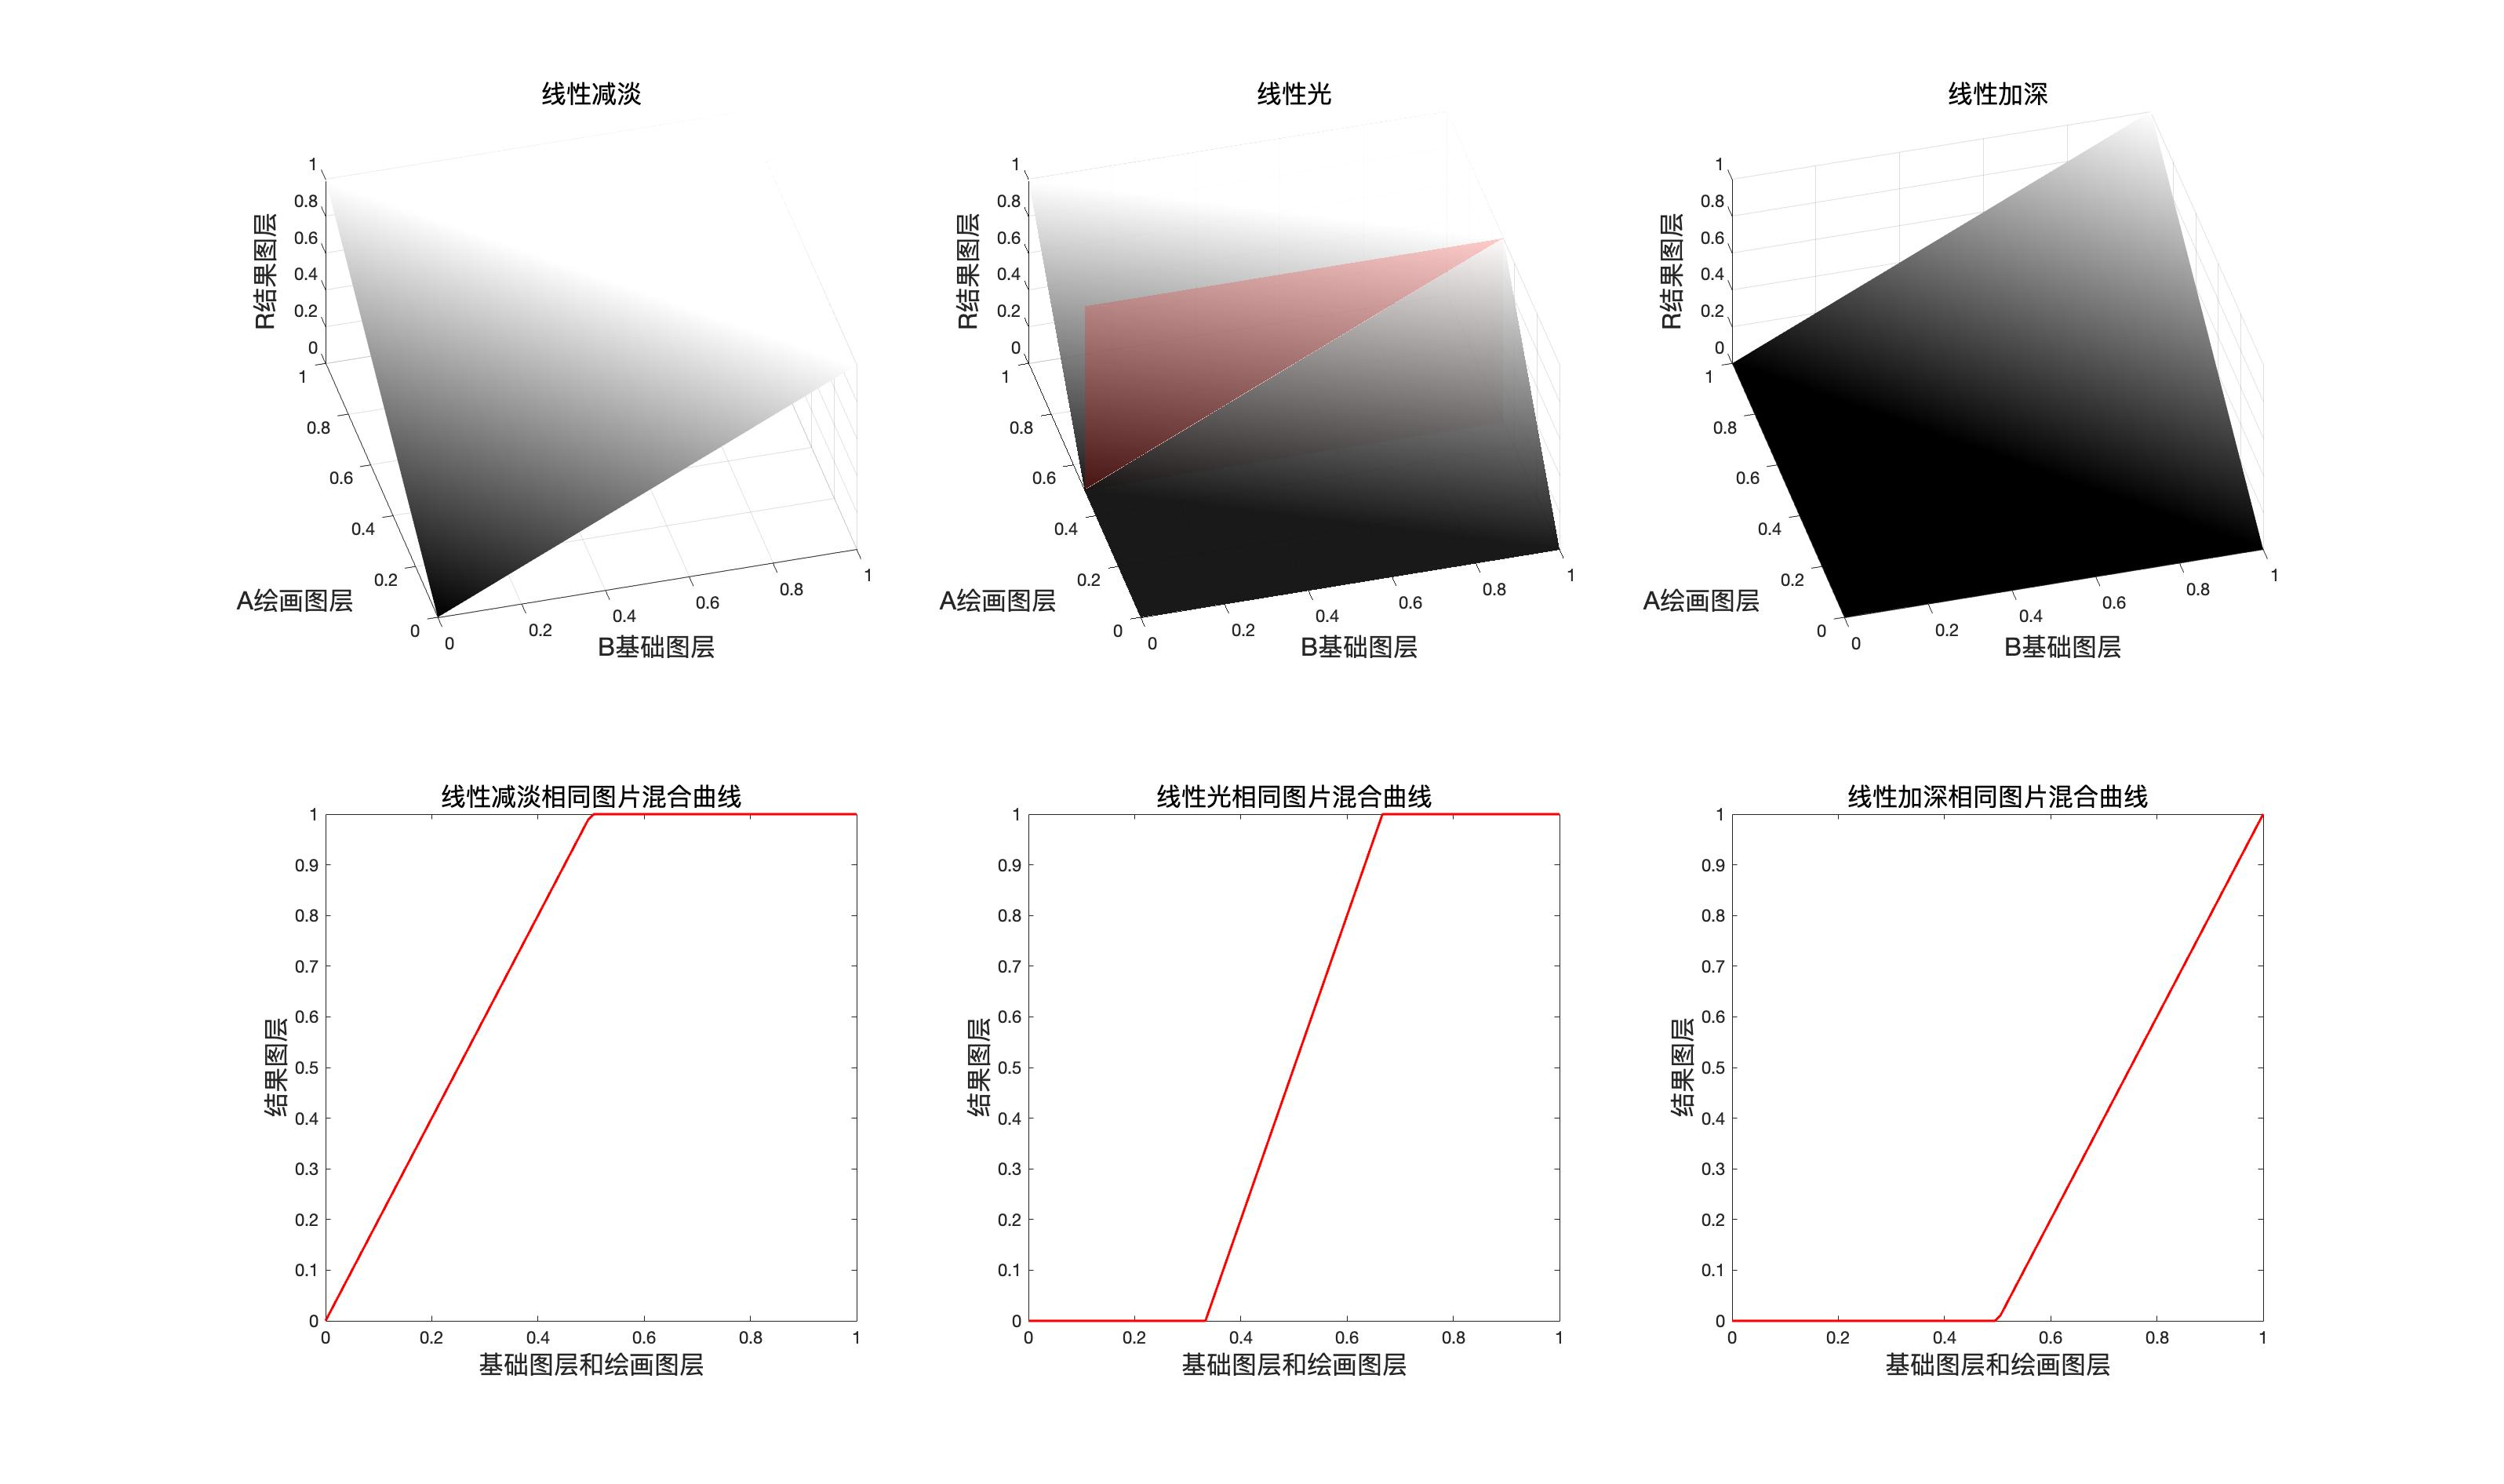
\includegraphics[width=\linewidth]{figure/线性光}
	\caption{}
	\label{fig:}
\end{figure}
\subsection{ 程序模拟该模式计算结果}

\begin{lstlisting}
	public static BlendColor LinearLight(BlendColor colorBase, BlendColor colorBlend, double fill, double opacity) {
		double red = LinearLightChannel(colorBase.red.get01Value(), colorBlend.red.get01Value(), fill);
		double green = LinearLightChannel(colorBase.green.get01Value(), colorBlend.green.get01Value(), fill);
		double blue = LinearLightChannel(colorBase.blue.get01Value(), colorBlend.blue.get01Value(), fill);
		return ColorUtils.Opacity(colorBase, new BlendColor(red * 255, green * 255, blue * 255), opacity);
	}
	
	private static double LinearLightChannel(double baseValue, double blendValue, double fill) {
		if (blendValue <= 0.5) {
			return LinearBurnChannel(baseValue, 2 * blendValue, fill);
		} else {
			return LinearDodgeChannel(baseValue, 2 * (blendValue  - 0.5), fill);
		}
	}
\end{lstlisting}

\begin{result}
\item 线 性 光(LinearLight)   RGB[ 88.20,  52.40,  73.68]~ HSY[324.34,  35.80,  65.48]~ HSB[324.34,  40.59,  34.59]
\end{result}

\subsection{ 验证}
% TODO: \usepackage{graphicx} required
\begin{figure}[h!]
	\centering
	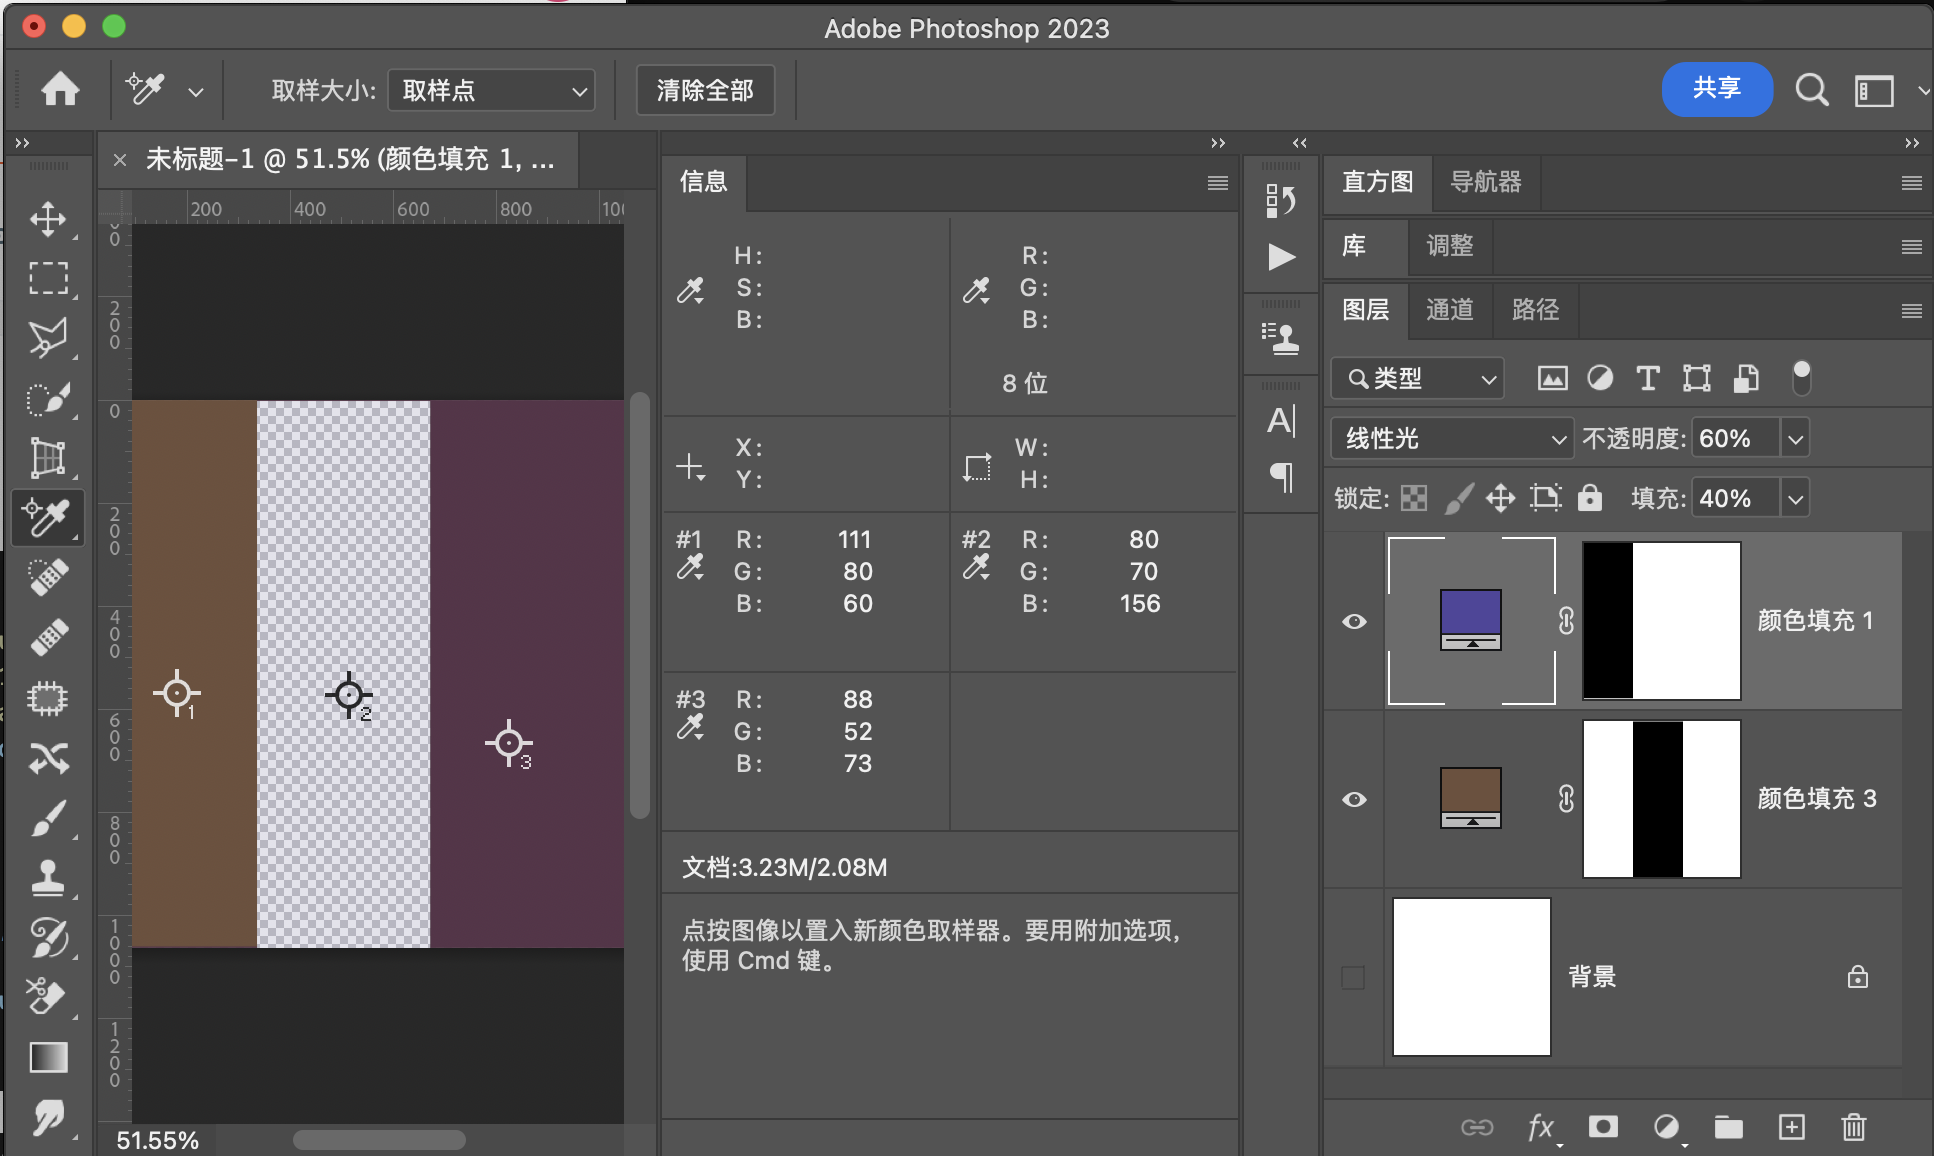
\includegraphics[width=\linewidth]{figure/linearllght}
	\caption{}
	\label{fig:linearllght}
\end{figure}

%
%\subsection{ 用途示例}
%
%1:组成中性灰磨皮

\newpage
\section{ 点光PinLight}

点光是变暗模式和变亮模式的组合

\subsection{ 公式}

\begin{equation}
	\begin{aligned}r=PinLight(b,a)&=\left\{ \begin{aligned}&Darken(b,2a)&a\leq 0.5\\&Lighten(b,2(a-0.5))&a> 0.5  \end{aligned}\right.=\left\{ \begin{aligned}&Min(b,2a)&a\leq 0.5\\&Max(b,2(a-0.5))&a> 0.5  \end{aligned}\right.\end{aligned}
	\end{equation}

\subsection{ 和填充结合}

\begin{equation}
	\begin{aligned}
		r= Fill(b,a)&=\left\{ \begin{aligned}&Min(b,2a\times fill)&a\leq 0.5\\&Max(b,2(a-0.5)\times fill)&a> 0.5  \end{aligned}\right.&
	\end{aligned}
	\end{equation}

\subsection{ 融合不透明度}

\begin{equation}
	r=Opacity(b,a)=op\times Fill(b,a)+(1-op)\times b
	\end{equation}

\subsection{ 映射面和同图等效曲线}
% TODO: \usepackage{graphicx} required
\begin{figure}[h!]
	\centering
	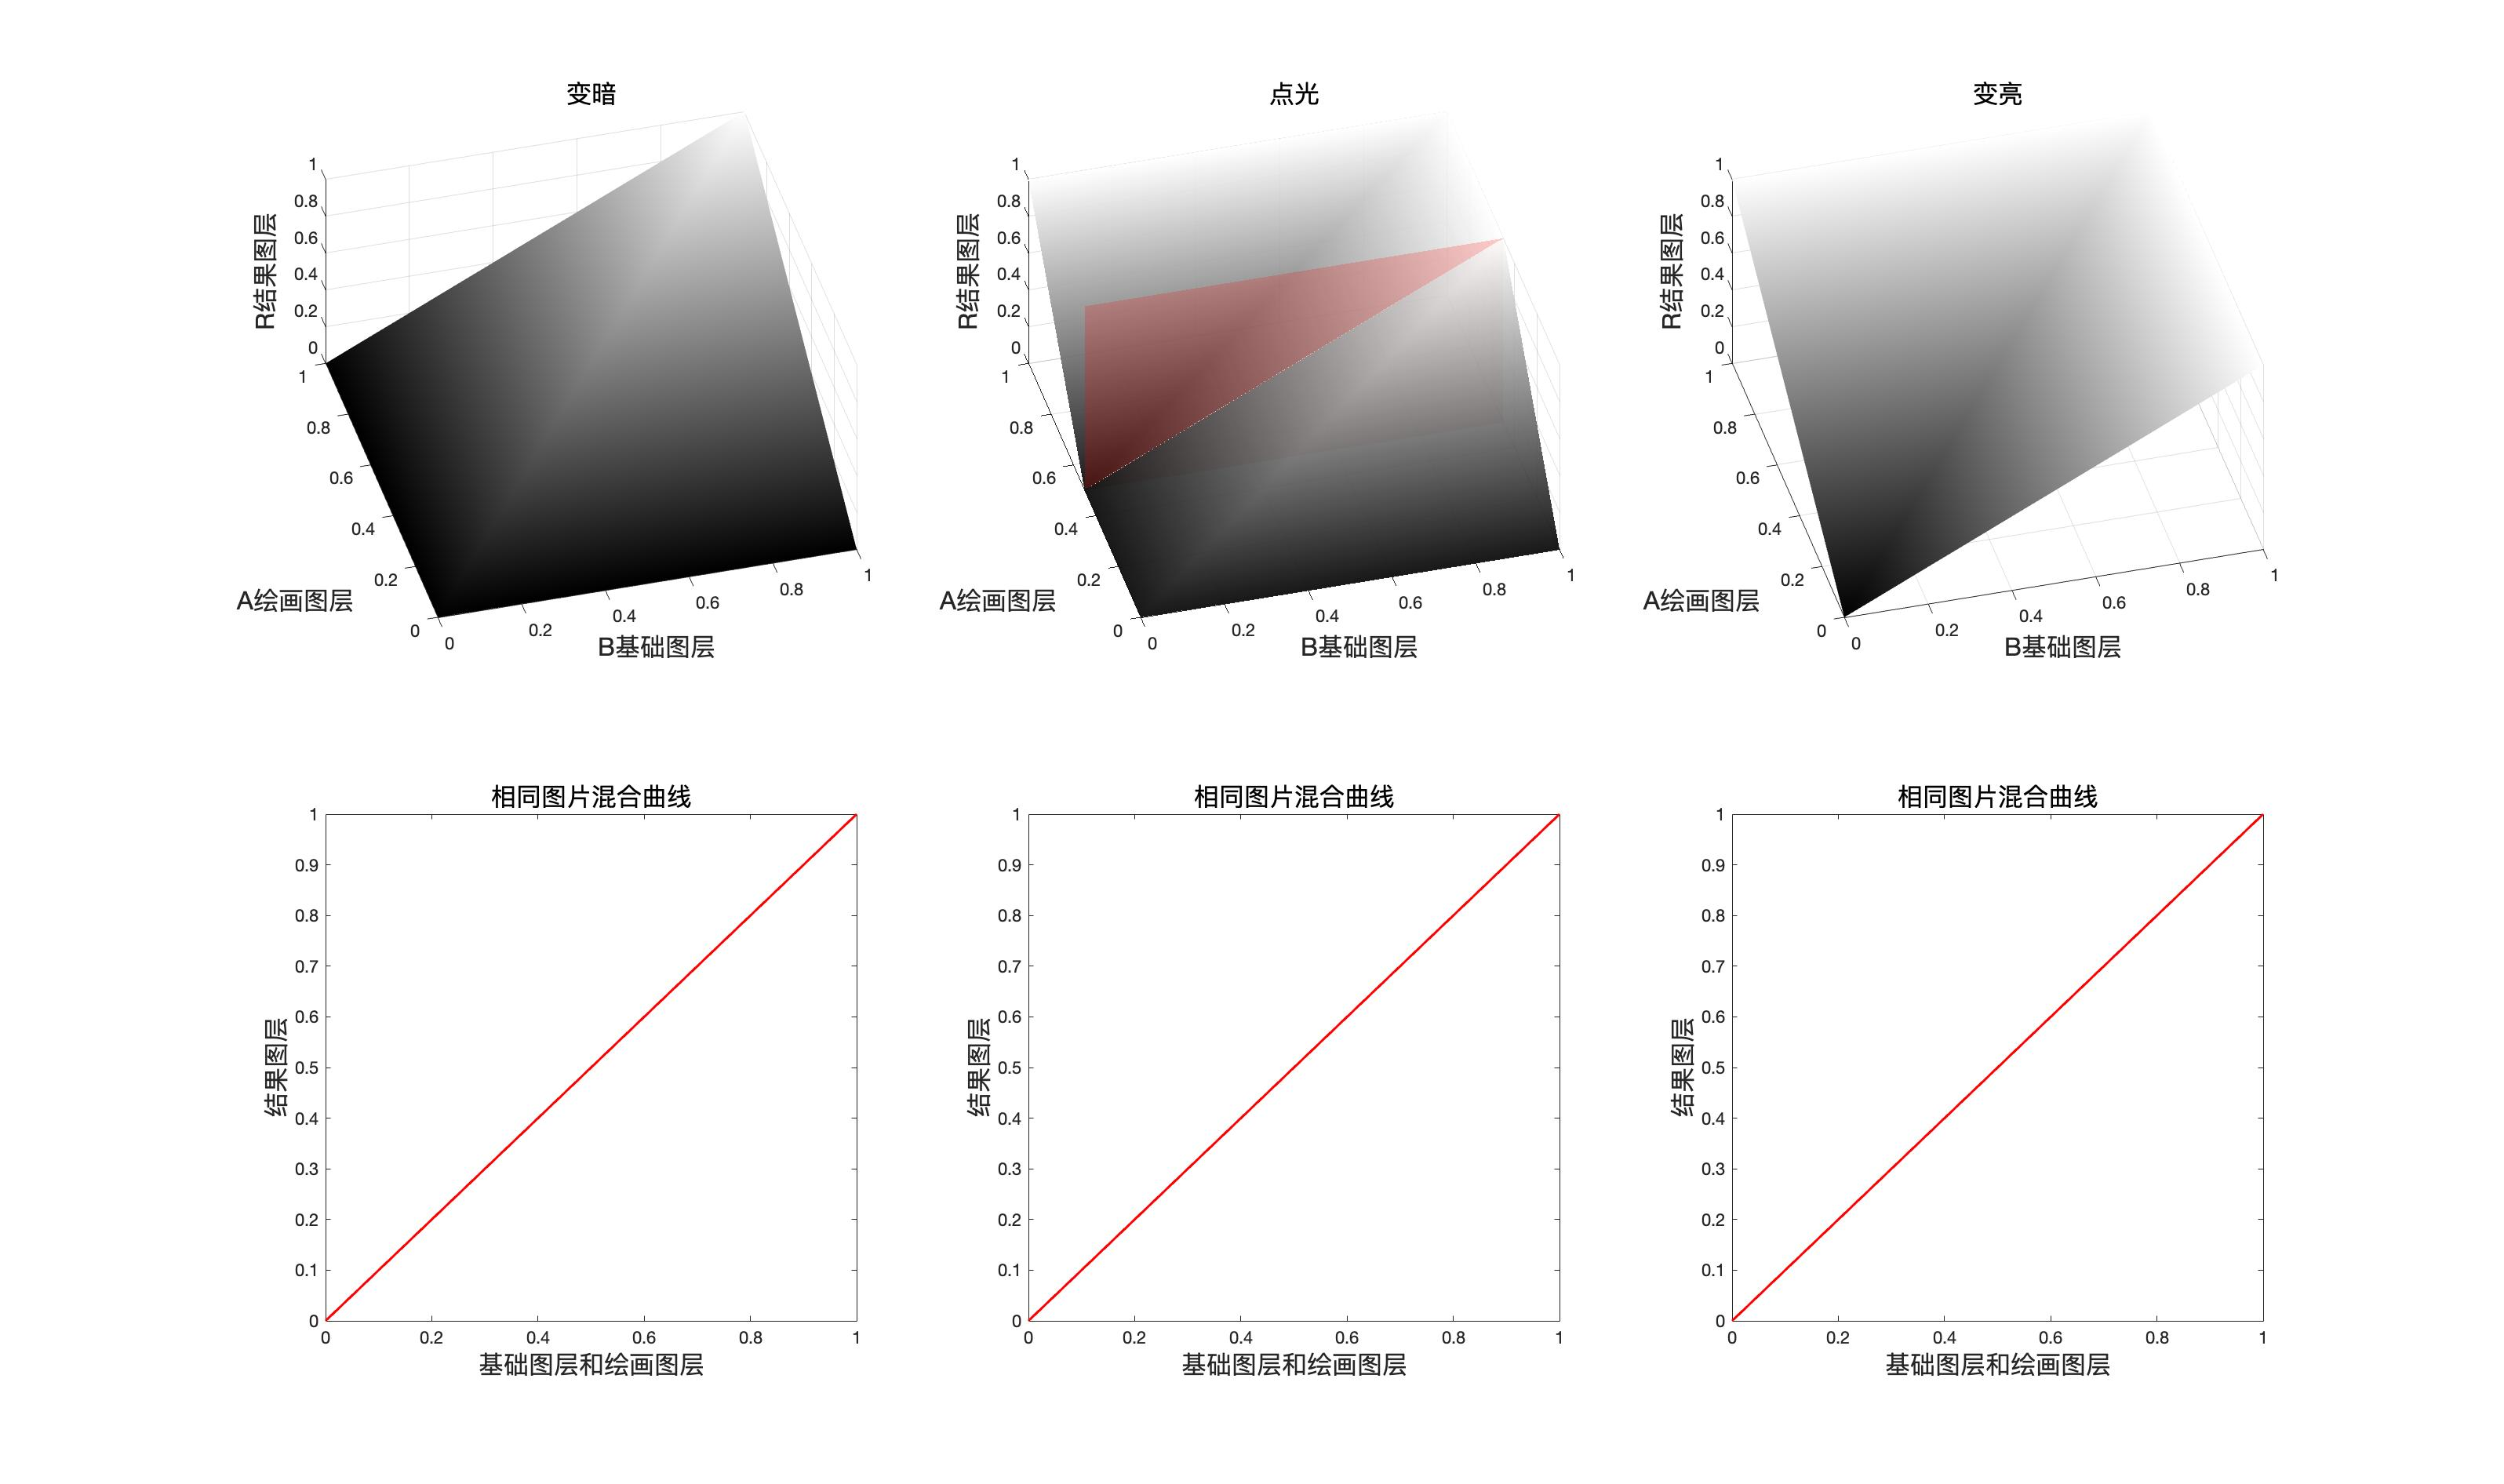
\includegraphics[width=\linewidth]{figure/点光}
	\caption{}
	\label{fig:}
\end{figure}



\subsection{ 程序模拟该模式计算结果}

\begin{lstlisting}
	// 点光
	public static BlendColor PinLight(BlendColor colorBase, BlendColor colorBlend, double fill, double opacity) {
		double red = PinLightChannel(colorBase.red.get01Value(), colorBlend.red.get01Value(), fill);
		double green = PinLightChannel(colorBase.green.get01Value(), colorBlend.green.get01Value(), fill);
		double blue = PinLightChannel(colorBase.blue.get01Value(), colorBlend.blue.get01Value(), fill);
		return ColorUtils.Opacity(colorBase, new BlendColor(red * 255, green * 255, blue * 255), opacity);
	}
	
	private static double PinLightChannel(double baseValue, double blendValue, double fill) {
		if (blendValue <= 0.5) {
			return DarkenChannel(baseValue, 2 * blendValue, fill);
		} else {
			return LightenChannel(baseValue, 2 * (blendValue  - 0.5), fill);
		}
	}
\end{lstlisting}


\begin{result}
\item 点    光(PinLight)      RGB[111.00,  80.00,  60.00]~ HSY[23.53,  51.00,  87.10 ]~ HSB[ 23.53,  45.95,  43.53]
\end{result}


\subsection{ 验证}

% TODO: \usepackage{graphicx} required
\begin{figure}[h!]
	\centering
	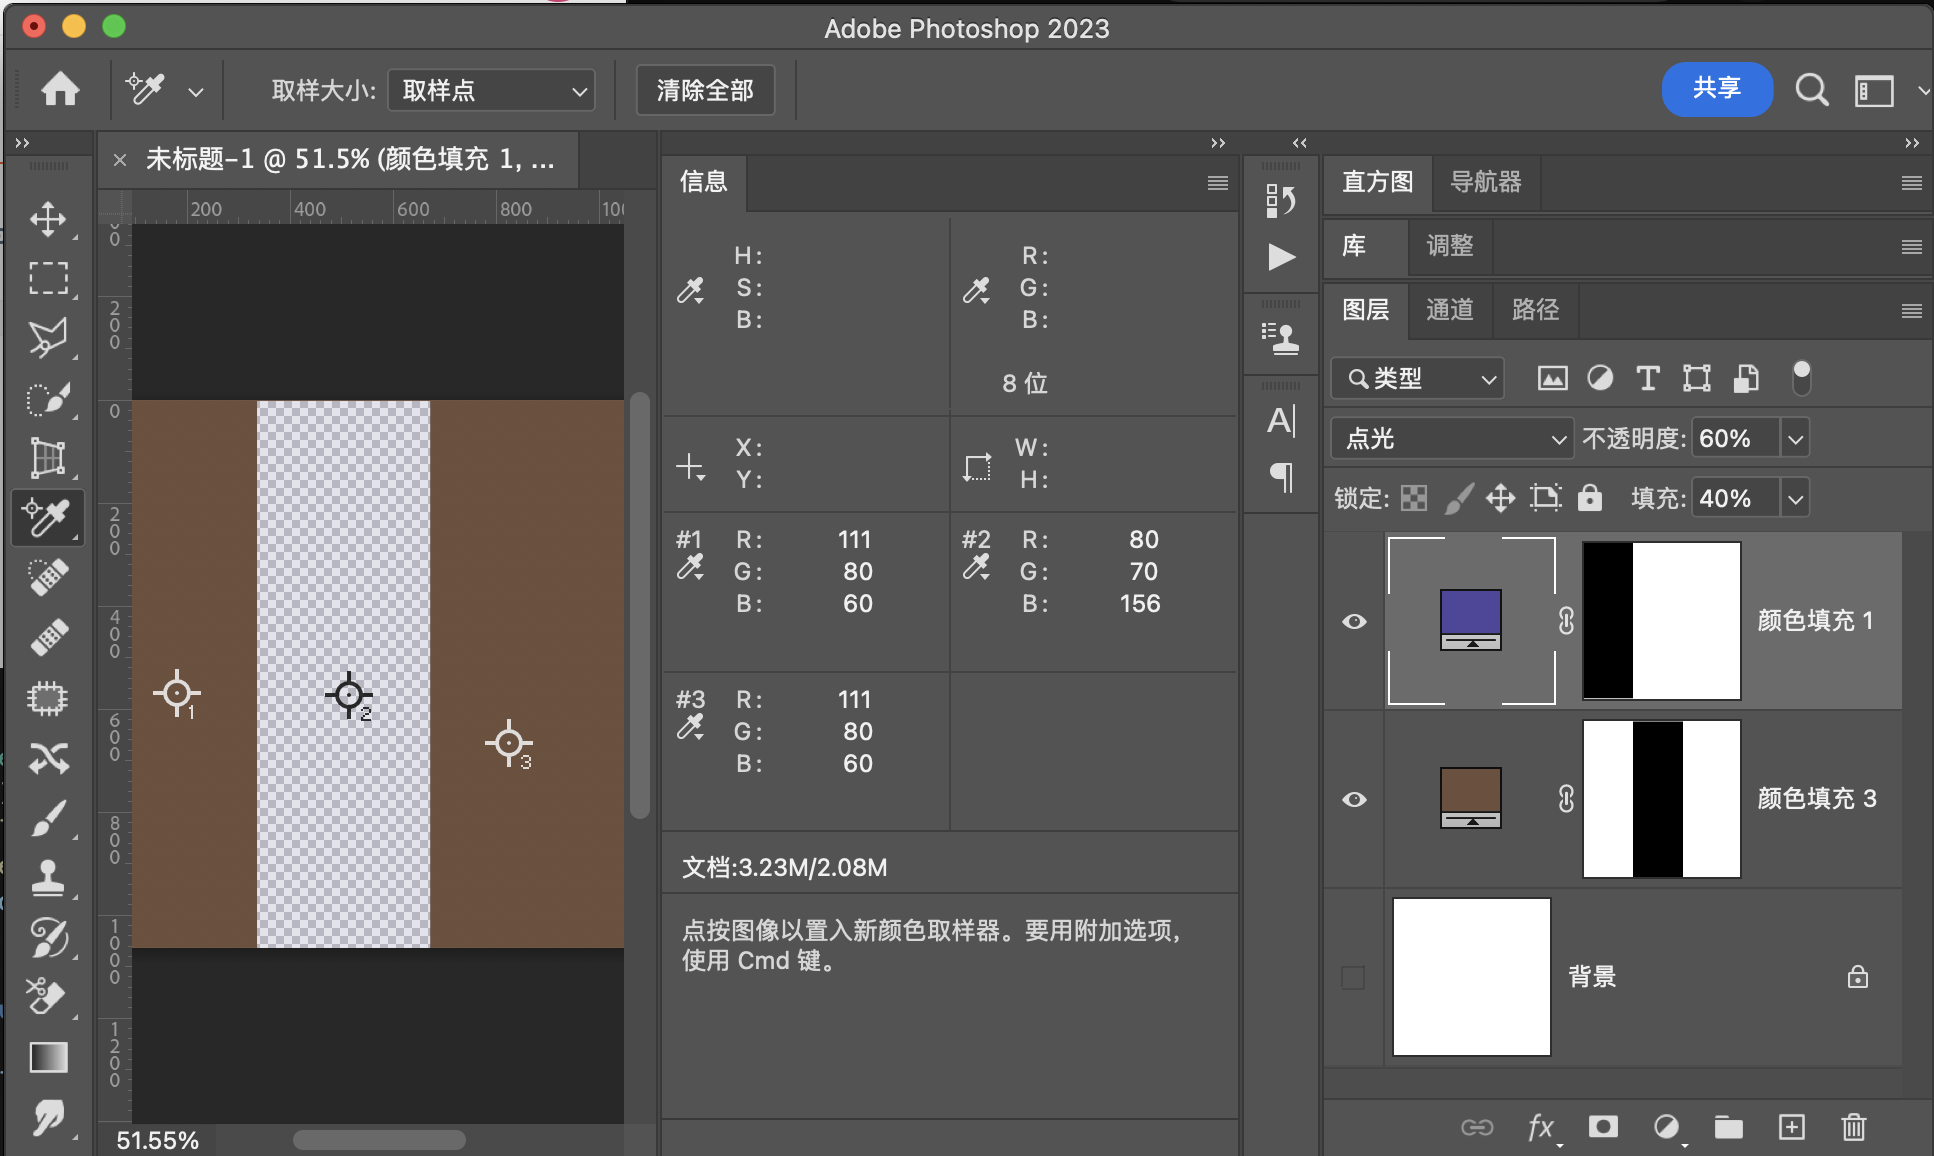
\includegraphics[width=\linewidth]{figure/pinlight}
	\caption{}
	\label{fig:pinlight}
\end{figure}

%\subsection{ 用途示例}
%
%1:增加图片对比度
\newpage
\section{ 亮光VividLight}

亮光模式是颜色加深和颜色减淡的组合

\subsection{ 公式}

\begin{equation}
	\begin{aligned}r=VividLight(b,a)&=\left\{ \begin{aligned}&ColorBurn(b,2a)&a\leq 0.5\\&ColorDodge(b,2(a-0.5))&a> 0.5 \end{aligned}\right.=\left\{ \begin{aligned}&1-\frac{(1-b)}{2a}&a\leq 0.5\\&\frac{b}{1-2(a-0.5)}&a>0.5\end{aligned}\right.\end{aligned}
	\end{equation}

\subsection{ 加上fill}

\begin{equation}
	\begin{aligned}r=FIll(b,a)&=\left\{ \begin{aligned}&ColorBurn(b,2a\times fill)&a\leq 0.5\\&ColorDodge(b,2(a-0.5)\times fill)&a> 0.5 \end{aligned}\right.=\left\{ \begin{aligned}&1-\frac{(1-b)}{2a\times fill}&a\leq 0.5\\&\frac{b}{1-2(a-0.5)\times fill}&a>0.5\end{aligned}\right.\end{aligned}
	\end{equation}

\subsection{ 融合不透明度}

\begin{equation}r=Opacity(b,a)=op\times Fill(b,a)+(1-op)\times b\end{equation}

\subsection{ 映射面和同图等效曲线}

% TODO: \usepackage{graphicx} required
\begin{figure}[h!]
	\centering
	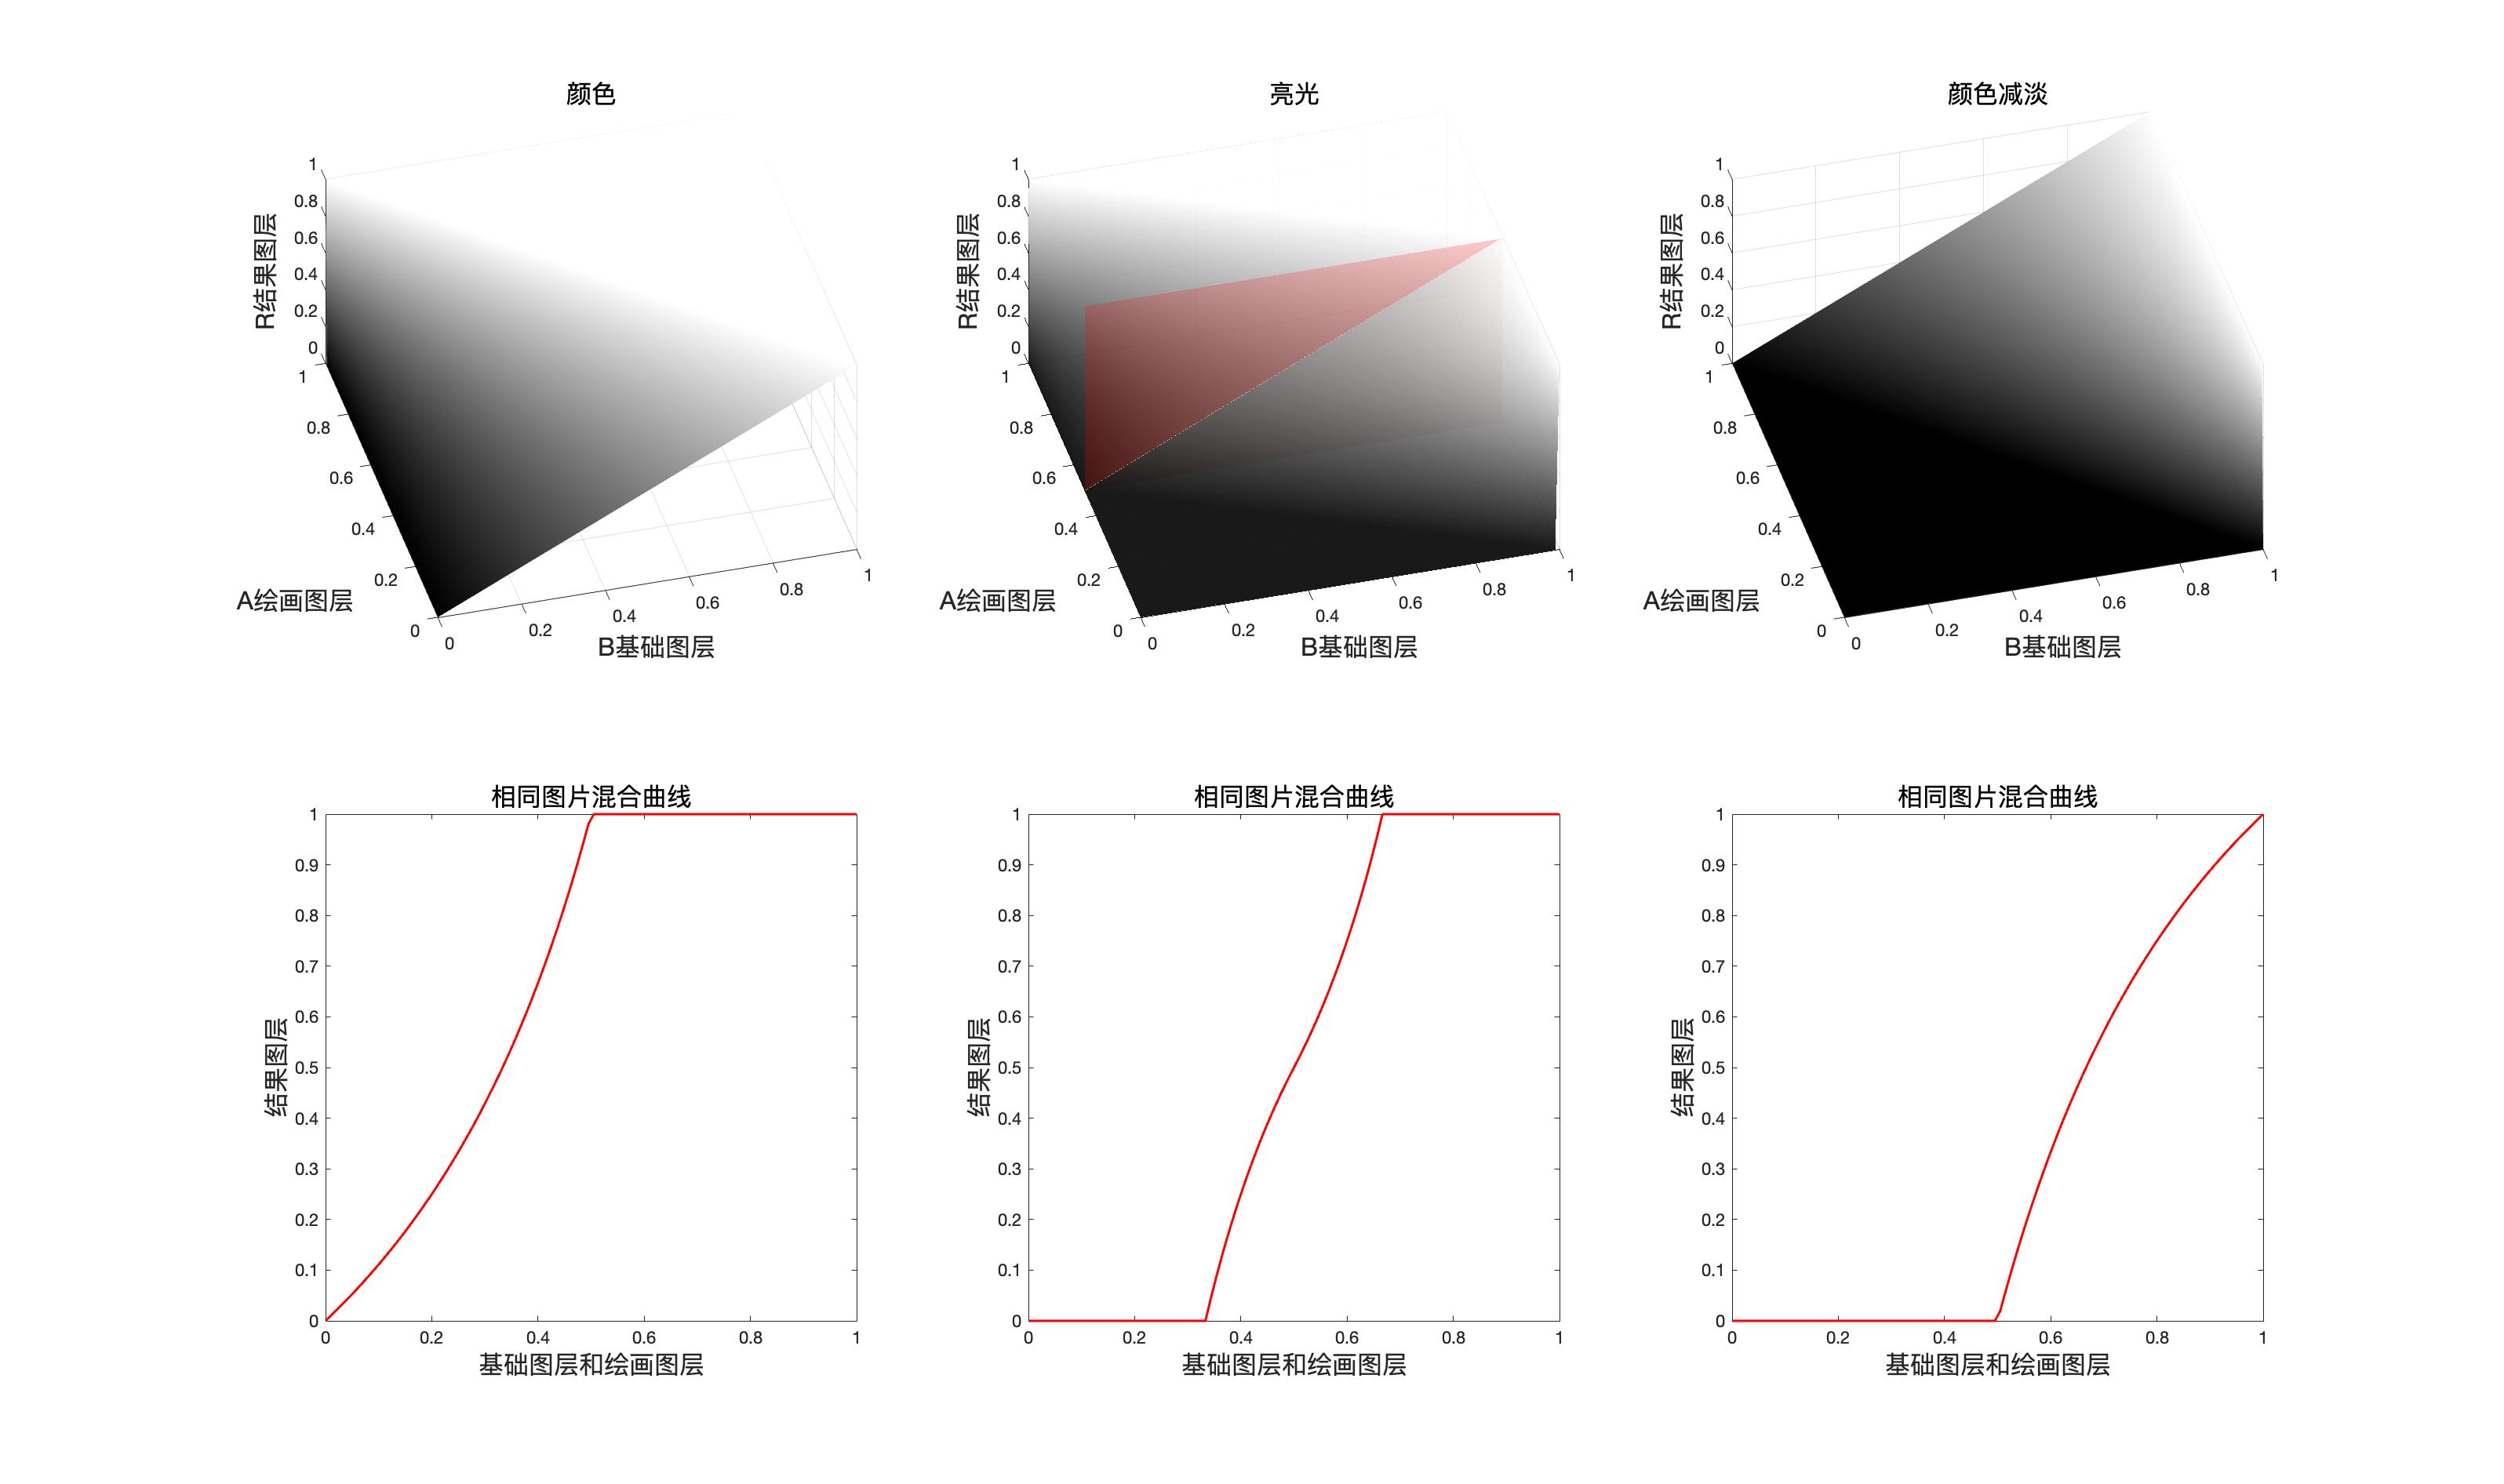
\includegraphics[width=\linewidth]{figure/亮光}
	\caption{}
	\label{fig:}
\end{figure}


\subsection{ 程序模拟该模式计算结果}
\begin{lstlisting}
	// 亮光
	public static BlendColor VividLight(BlendColor colorBase, BlendColor colorBlend, double fill, double opacity) {
		double red = VividLightChannel(colorBase.red.get01Value(), colorBlend.red.get01Value(), fill);
		double green = VividLightChannel(colorBase.green.get01Value(), colorBlend.green.get01Value(), fill);
		double blue = VividLightChannel(colorBase.blue.get01Value(), colorBlend.blue.get01Value(), fill);
		return ColorUtils.Opacity(colorBase, new BlendColor(red * 255, green * 255, blue * 255), opacity);
	}
	
	private static double VividLightChannel(double baseValue, double blendValue, double fill) {
		if (blendValue <= 0.5) {
			return ColorBurnChannel(baseValue, 2 * blendValue, fill);
		} else {
			return ColorDodgeChannel(baseValue, 2 * (blendValue  - 0.5), fill);
		}
	}
\end{lstlisting}



\begin{result}
\item 亮    光(VividLight)    RGB[ 95.87,  56.89,  63.53]~ HSY[349.77,  38.98,  69.31]~ HSB[349.77,  40.66,  37.60]
\end{result}


\subsection{ 验证}
% TODO: \usepackage{graphicx} required
\begin{figure}[h!]
	\centering
	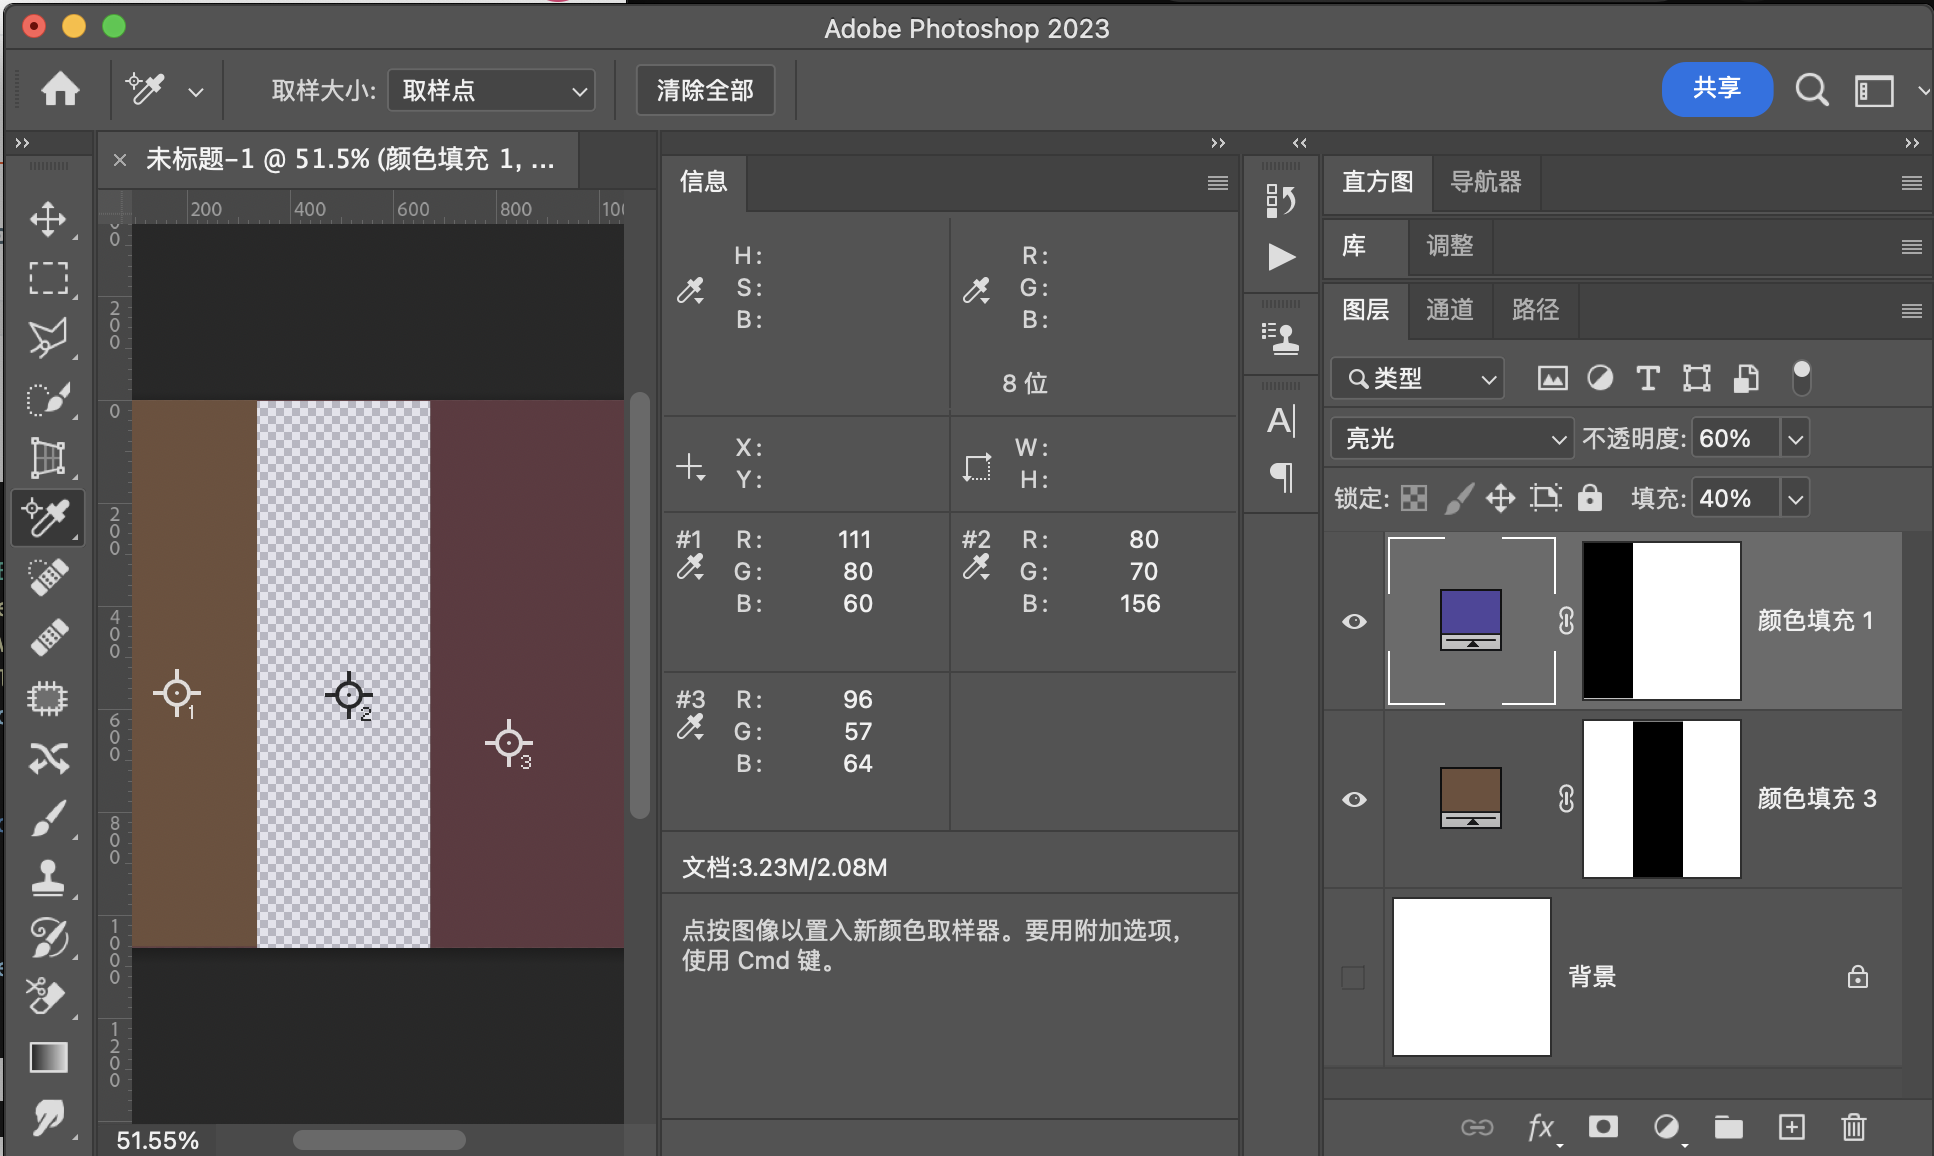
\includegraphics[width=\linewidth]{figure/vividlight}
	\caption{}
	\label{fig:vividlight}
\end{figure}


%
%\subsection{ 用途示例}
%
%1:同图混合增加图片对比度
%2:通道抠图法,去除白边

\newpage
\section{ 实色混合HardMix}

实色混合是一种极端的混合方式,但是如果它合填充结合,则它会产生一些意想不到的效果,并且我们还能找到它合线性光的关系

\subsection{ 公式}
\begin{equation}r=HardMix(b,a)=\left\{ \begin{aligned}&1&b+a\geq 1\\&0&else  \end{aligned}\right.\end{equation}

由公式我们可以看出,最后的结果只有两个,所以最后之后保留$2^3=8$种颜色,也就是

	 (0,0,0)黑,(1,0,0)红,(1,1,0)黄,(1,1,1)白,
	 (0,1,0)绿,(0,1,1)青,(1,0,1)品红,(0,0,1)蓝
\subsection{ 加上fill}
但是如果填充介入表达式,则结果将合线性光类似
\begin{equation}r=HardMix_{fill}(b,a)=\left\{ \begin{aligned}&0&  \frac{fill\times a+b-fill}{(1-fill)}<0\\ &\frac{fill\times a+b-fill}{(1-fill)}&0\leq \frac{fill\times a+b-fill}{(1-fill)}\leq 1\\ &1&  \frac{fill\times a+b-fill}{(1-fill)}>1 \end{aligned}\right.\end{equation}

如果fill的取值是$0.5$则
\begin{equation}\begin{aligned}r=HardMix_{fill}(b,a)=&\left\{ \begin{aligned}&0&  \frac{0.5\times a+b-0.5}{(1-0.5)}<0\\ &\frac{0.5\times a+b-0.5}{(1-0.5)}&0\leq \frac{0.5\times a+b-0.5}{(1-0.5)}\leq 1\\&1&  \frac{0.5\times a+b-0.5}{(1-0.5)}>1  \end{aligned}\right.\\=&\left\{ \begin{aligned}&0&  a+2b-1<0\\ &a+2b-1&0\leq a+2b-1\leq 1\\ &1&  a+2b-1>1    \end{aligned}\right.\end{aligned}\end{equation}
\begin{notice}
\item 上面的结果就是线性光的表达式,也就是说此时二者等价,或者说是互逆,也就是说,实色混合其实是线性光的强化版本,可以实现线性光的功能而去变化更多。
\end{notice}


\subsection{ 融合不透明度}

\begin{equation}r=Opacity(b,a)=op\times HardMix_{fill}(b,a)+(1-op)\times b\end{equation}

\subsection{ 映射面和同图等效曲线}

由此我们可以看出,实色混合可以看作线性减淡和线性加深的组合,
也可以看作是颜色减淡和颜色加深的组合,注意这里是可以看作,并不是真的。

% TODO: \usepackage{graphicx} required
\begin{figure}[h!]
	\centering
	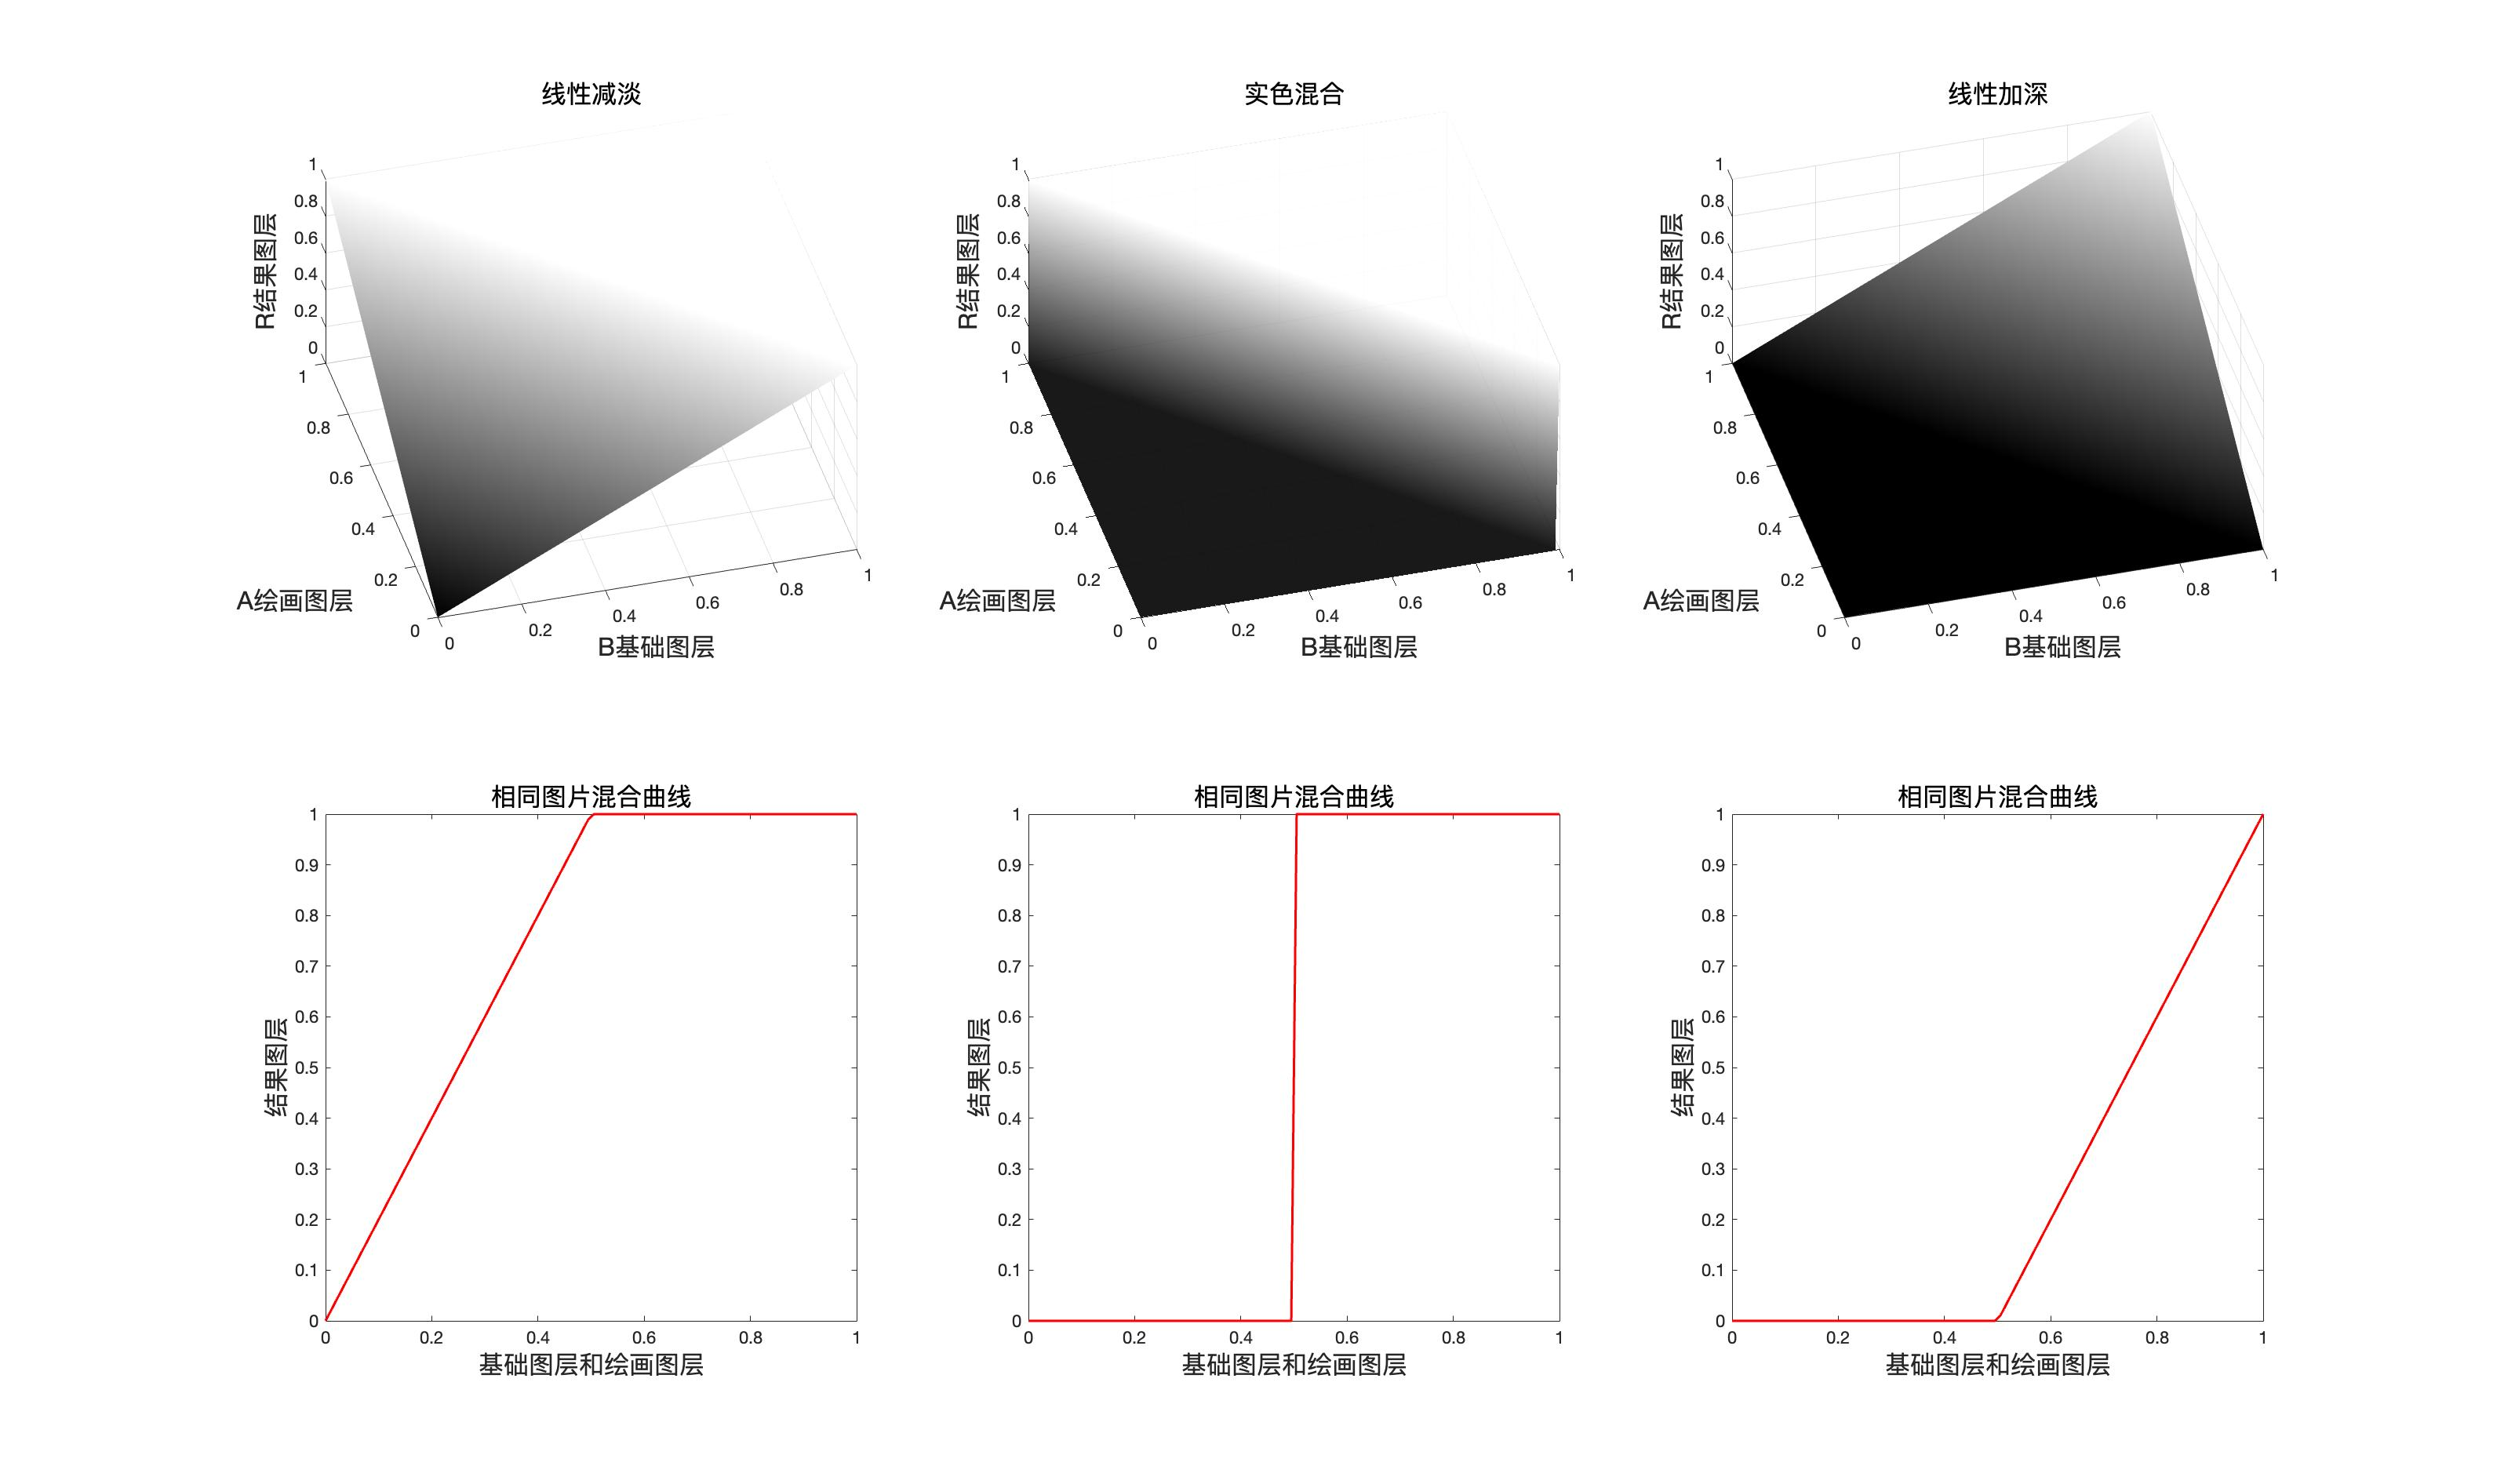
\includegraphics[width=\linewidth]{figure/试色线性混合}
	\caption{}
	\label{fig:}
\end{figure}



线性减淡和线性加深组合方式(真的)
% TODO: \usepackage{graphicx} required
\begin{figure}[h!]
	\centering
	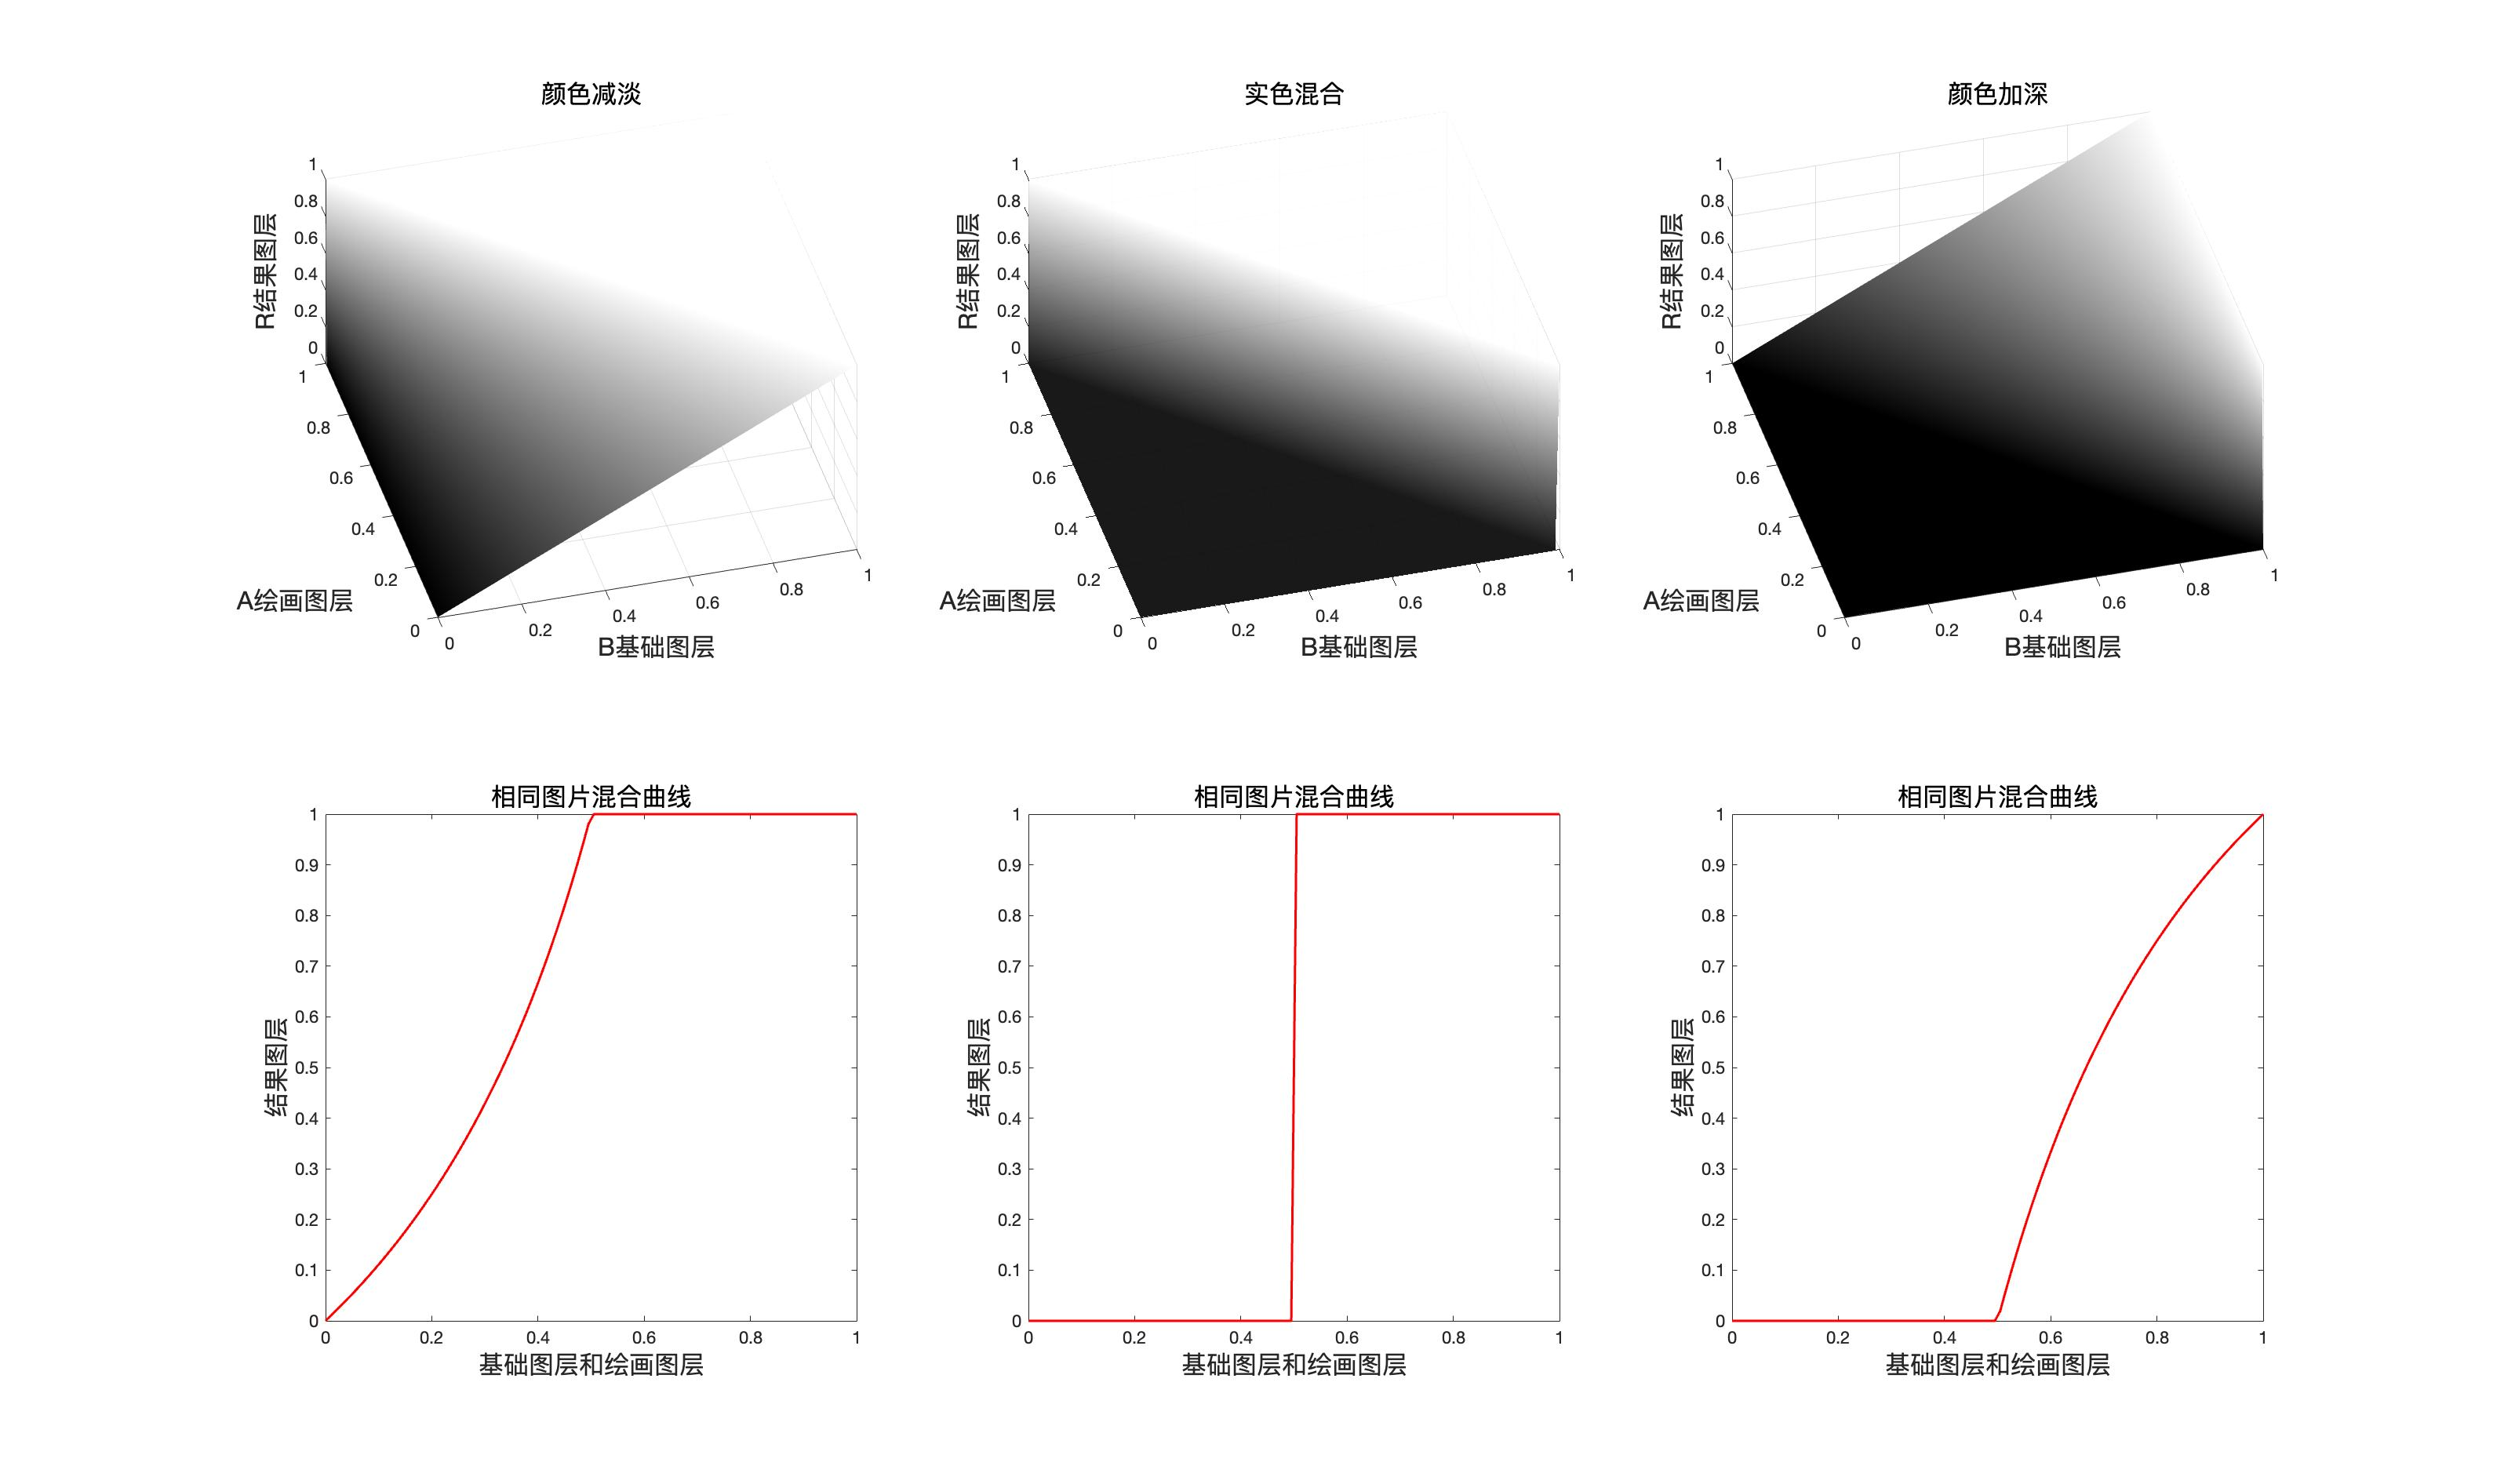
\includegraphics[width=\linewidth]{figure/试色颜色混合}
	\caption{}
	\label{fig:}
\end{figure}



颜色减淡和颜色加深的组合方式(可以看作是这样)


\begin{notice}
	\item 由我们刚才推导出当填充等于$50\%$的时候,他可以和线性光互逆,此时我们也可以得出结论,实色混合本质是一种特殊的线性减淡和线性加深的组合,并且线性光是实色混合的特殊形式。
\end{notice}
\subsection{ 程序模拟该模式计算结果}

\begin{lstlisting}
	// 实色混合
	public static BlendColor HardMix(BlendColor colorBase, BlendColor colorBlend, double fill, double opacity) {
		double red = HardMixChannel(colorBase.red.get01Value(), colorBlend.red.get01Value(), fill);
		double green = HardMixChannel(colorBase.green.get01Value(), colorBlend.green.get01Value(), fill);
		double blue = HardMixChannel(colorBase.blue.get01Value(), colorBlend.blue.get01Value(), fill);
		return ColorUtils.Opacity(colorBase, new BlendColor(red * 255, green * 255, blue * 255), opacity);
	}
	
	private static double HardMixChannel(double baseValue, double blendValue, double fill) {
		if (fill == 1) {
			if (baseValue + blendValue >= 0.5) {
				return 1;
			}
			return 0;
		}
		return ColorUtils.round((fill * blendValue + baseValue  fill) / (1 - fill), 1, 0);
	}
\end{lstlisting}



\begin{result}
\item 实色混合(HardMix)       RGB[ 85.40,  38.00,  44.40]~ HSY[351.90,  47.40,  52.92]~ HSB[351.90,  55.50,  33.49]
\end{result}
\newpage
\subsection{ 验证}
% TODO: \usepackage{graphicx} required
\begin{figure}[h!]
	\centering
	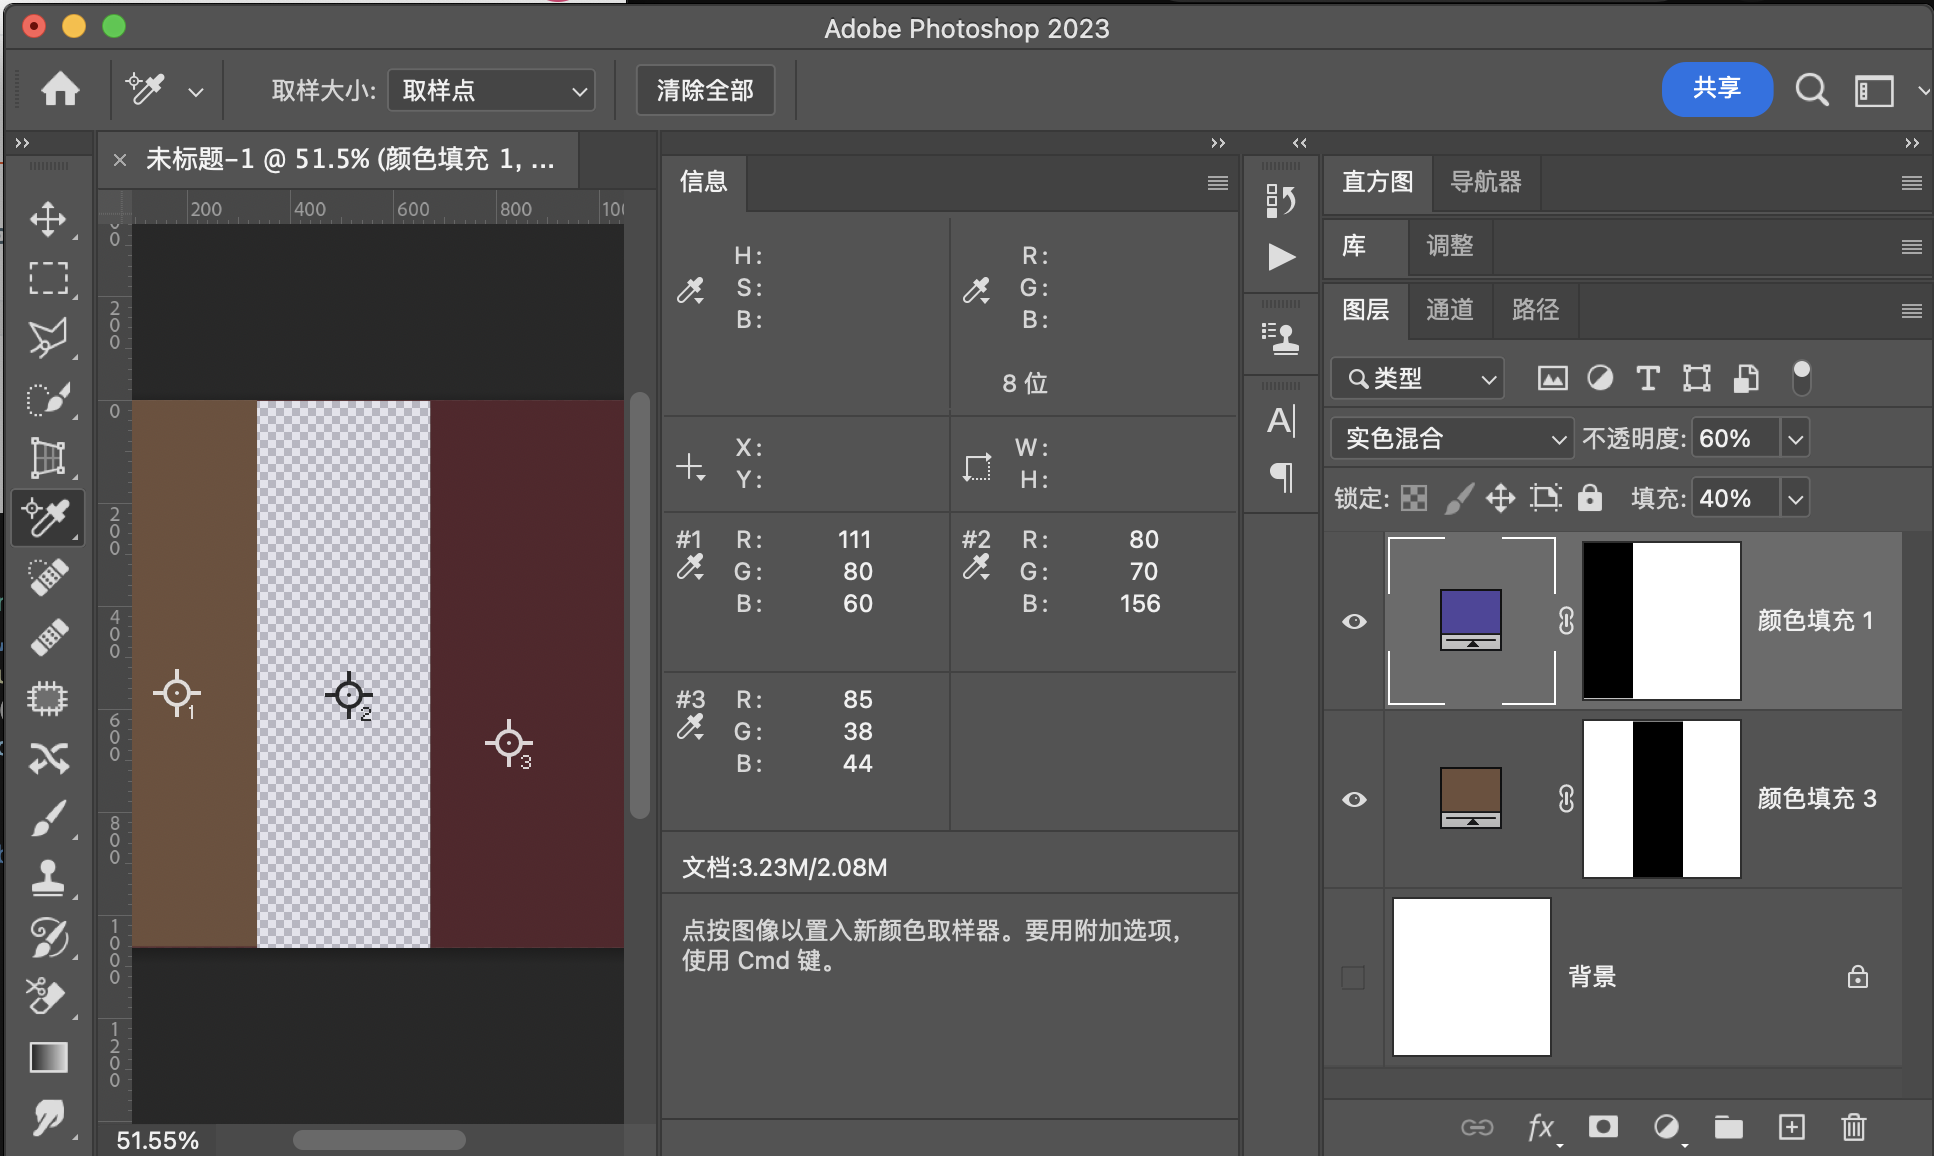
\includegraphics[width=\linewidth]{figure/hardmix}
	\caption{}
	\label{fig:hardmix}
\end{figure}
%
%\subsection{ 用途示例}
%
%1:同图混合增加图片对比度
%
%2:特殊光效,可以根据fill调节

\chapter{差值组}

\section{ 差值Difference}

差值就是基础图层和混合图层的差值的绝对值

\subsection{ 公式}
\begin{equation}r=Difference(b,a)=|b-a|\end{equation}
\subsection{ 结合填充}
\begin{equation}r=Fill(b,a)=|b-a|\times fill + (1-fill)\times b\end{equation}
\subsection{ 融合不透明度}
\begin{equation}r=Opacity(b,a)=op\times Fill(b,a)+(1-op)\times b\end{equation}
\subsection{ 映射面和同图等效曲线}
% TODO: \usepackage{graphicx} required
\begin{figure}[h!]
	\centering
	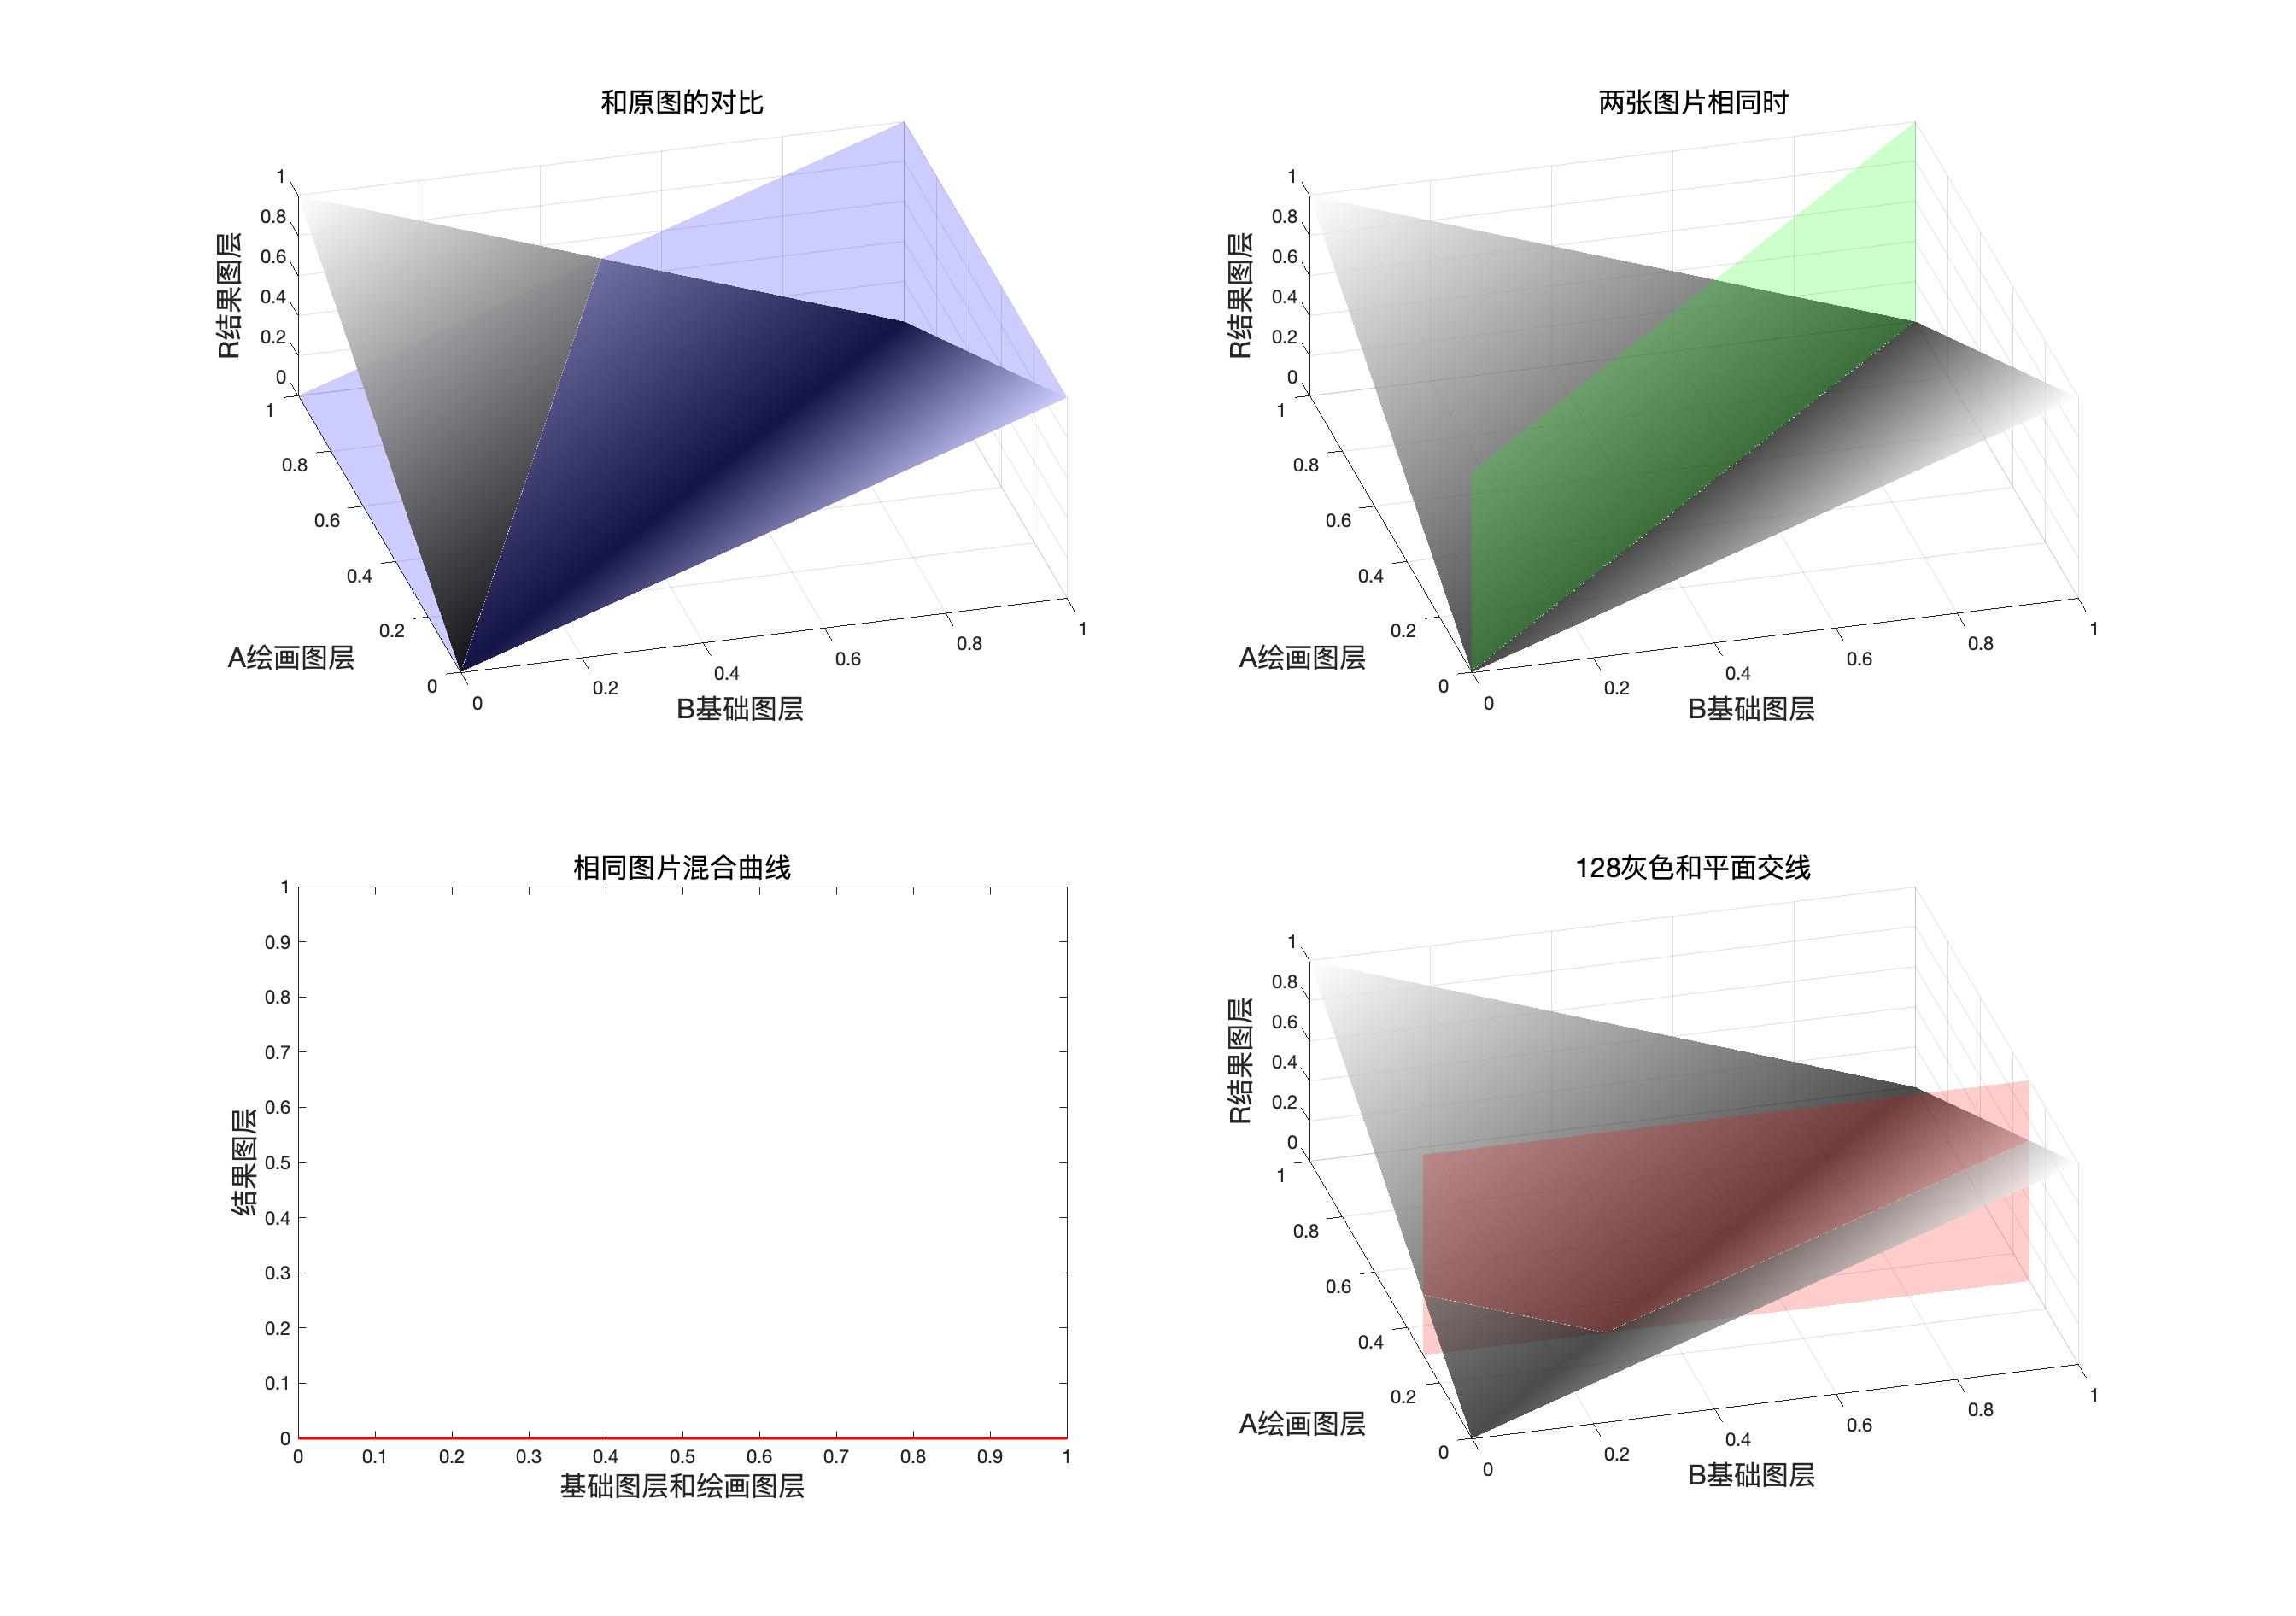
\includegraphics[width=0.9\linewidth]{figure/差值}
	\caption{}
	\label{fig:}
\end{figure}



\subsection{ 程序模拟该模式计算结果}

\begin{lstlisting}
	// 差值
	public static BlendColor Difference(BlendColor colorBase, BlendColor colorBlend, double fill, double opacity) {
		double red = DifferenceChannel(colorBase.red.get01Value(), colorBlend.red.get01Value(), fill);
		double green = DifferenceChannel(colorBase.green.get01Value(), colorBlend.green.get01Value(), fill);
		double blue = DifferenceChannel(colorBase.blue.get01Value(), colorBlend.blue.get01Value(), fill);
		return ColorUtils.Opacity(colorBase, new BlendColor(red * 255, green * 255, blue * 255), opacity);
	}
	
	private static double DifferenceChannel(double baseValue, double blendValue, double fill) {
		return ColorUtils.round(Math.abs(baseValue  blendValue * fill), 1, 0);
	}
\end{lstlisting}
\begin{result}
	\item 差    值(Difference)    RGB[ 91.80,  63.20,  25.44]~ HSY[34.14,  66.36,  67.63 ]~ HSB[ 34.14,  72.29,  36.00]
\end{result}
\subsection{ 验证}
% TODO: \usepackage{graphicx} required
\begin{figure}[h!]
	\centering
	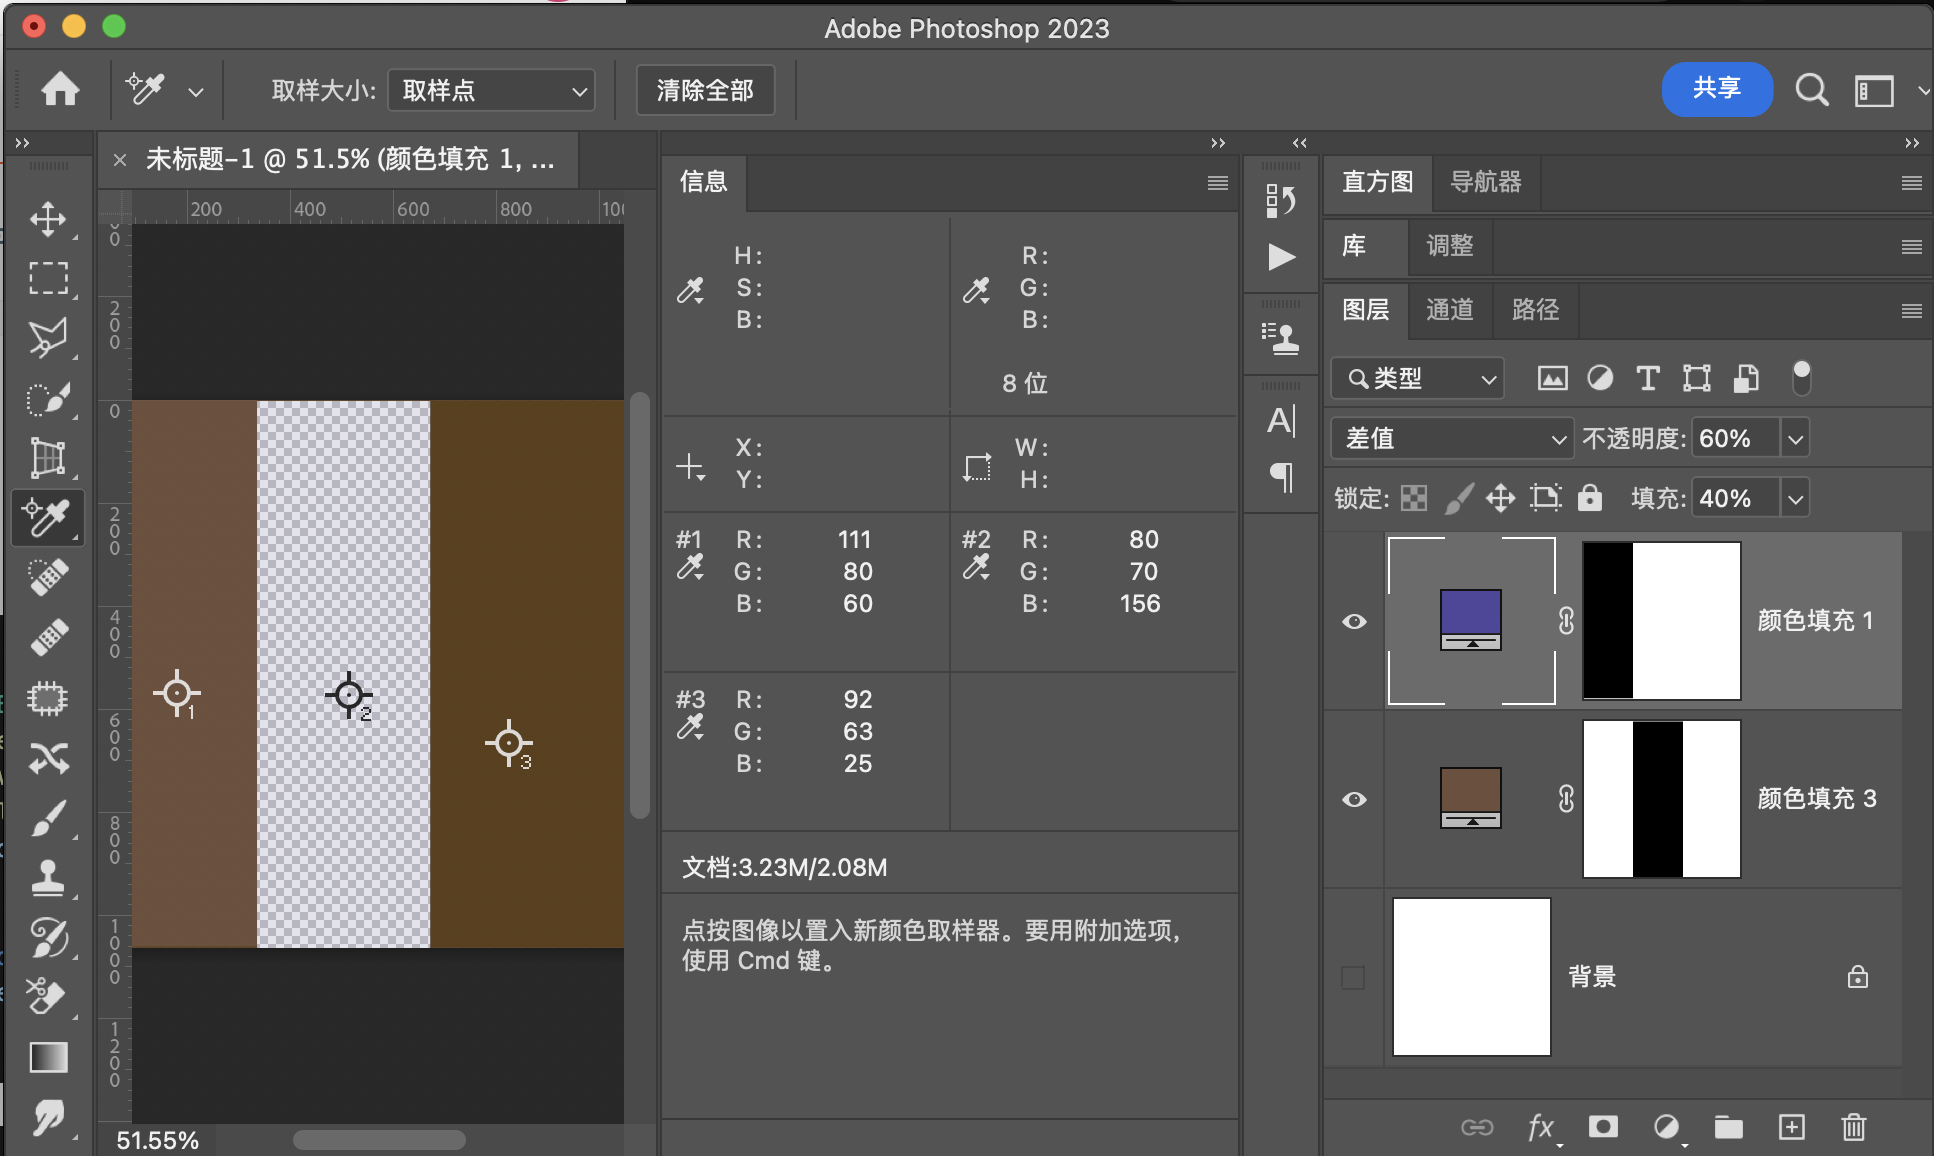
\includegraphics[width=\linewidth]{figure/difference}
	\caption{}
	\label{fig:difference}
\end{figure}
%
%\subsection{ 用途示例}
%
%1:对齐图片
%2:颜色矫正

\section{ 排除Exclusion}

\subsection{ 公式}

\begin{equation}r=Exclusion(b,a)=b+a-2ba\end{equation}

\subsection{ 结合填充}

\begin{equation}r=Fill(b,a)=(b+a-2ba)\times fill + (1-fill)\times b\end{equation}

\subsection{ 融合不透明度}

\begin{equation}r=Opacity(b,a)=op\times Fill(b,a)+(1-op)\times b\end{equation}

\subsection{ 如果在该模式下,混合图层是白色,黑色或者中性灰色}

\penmark{\textbf{ 白色}}

\begin{equation}r=Exclusion(b,1)=b+1-2b\times 1=1-b\end{equation}

等于负片

\penmark{\textbf{ 黑色}}

\begin{equation}r=Exclusion(b,0)=b+1-2b\times 0=b\end{equation}

等于原图

\penmark{\textbf{ 中性灰}}

\begin{equation}r=Exclusion(b,\dfrac{1}{2})=b+\dfrac{1}{2}-2b\times \dfrac{1}{2}=\dfrac{1}{2}\end{equation}

依然是中性灰
\newpage
\subsection{ 映射面和同图等效曲线}
% TODO: \usepackage{graphicx} required
\begin{figure}[h!]
	\centering
	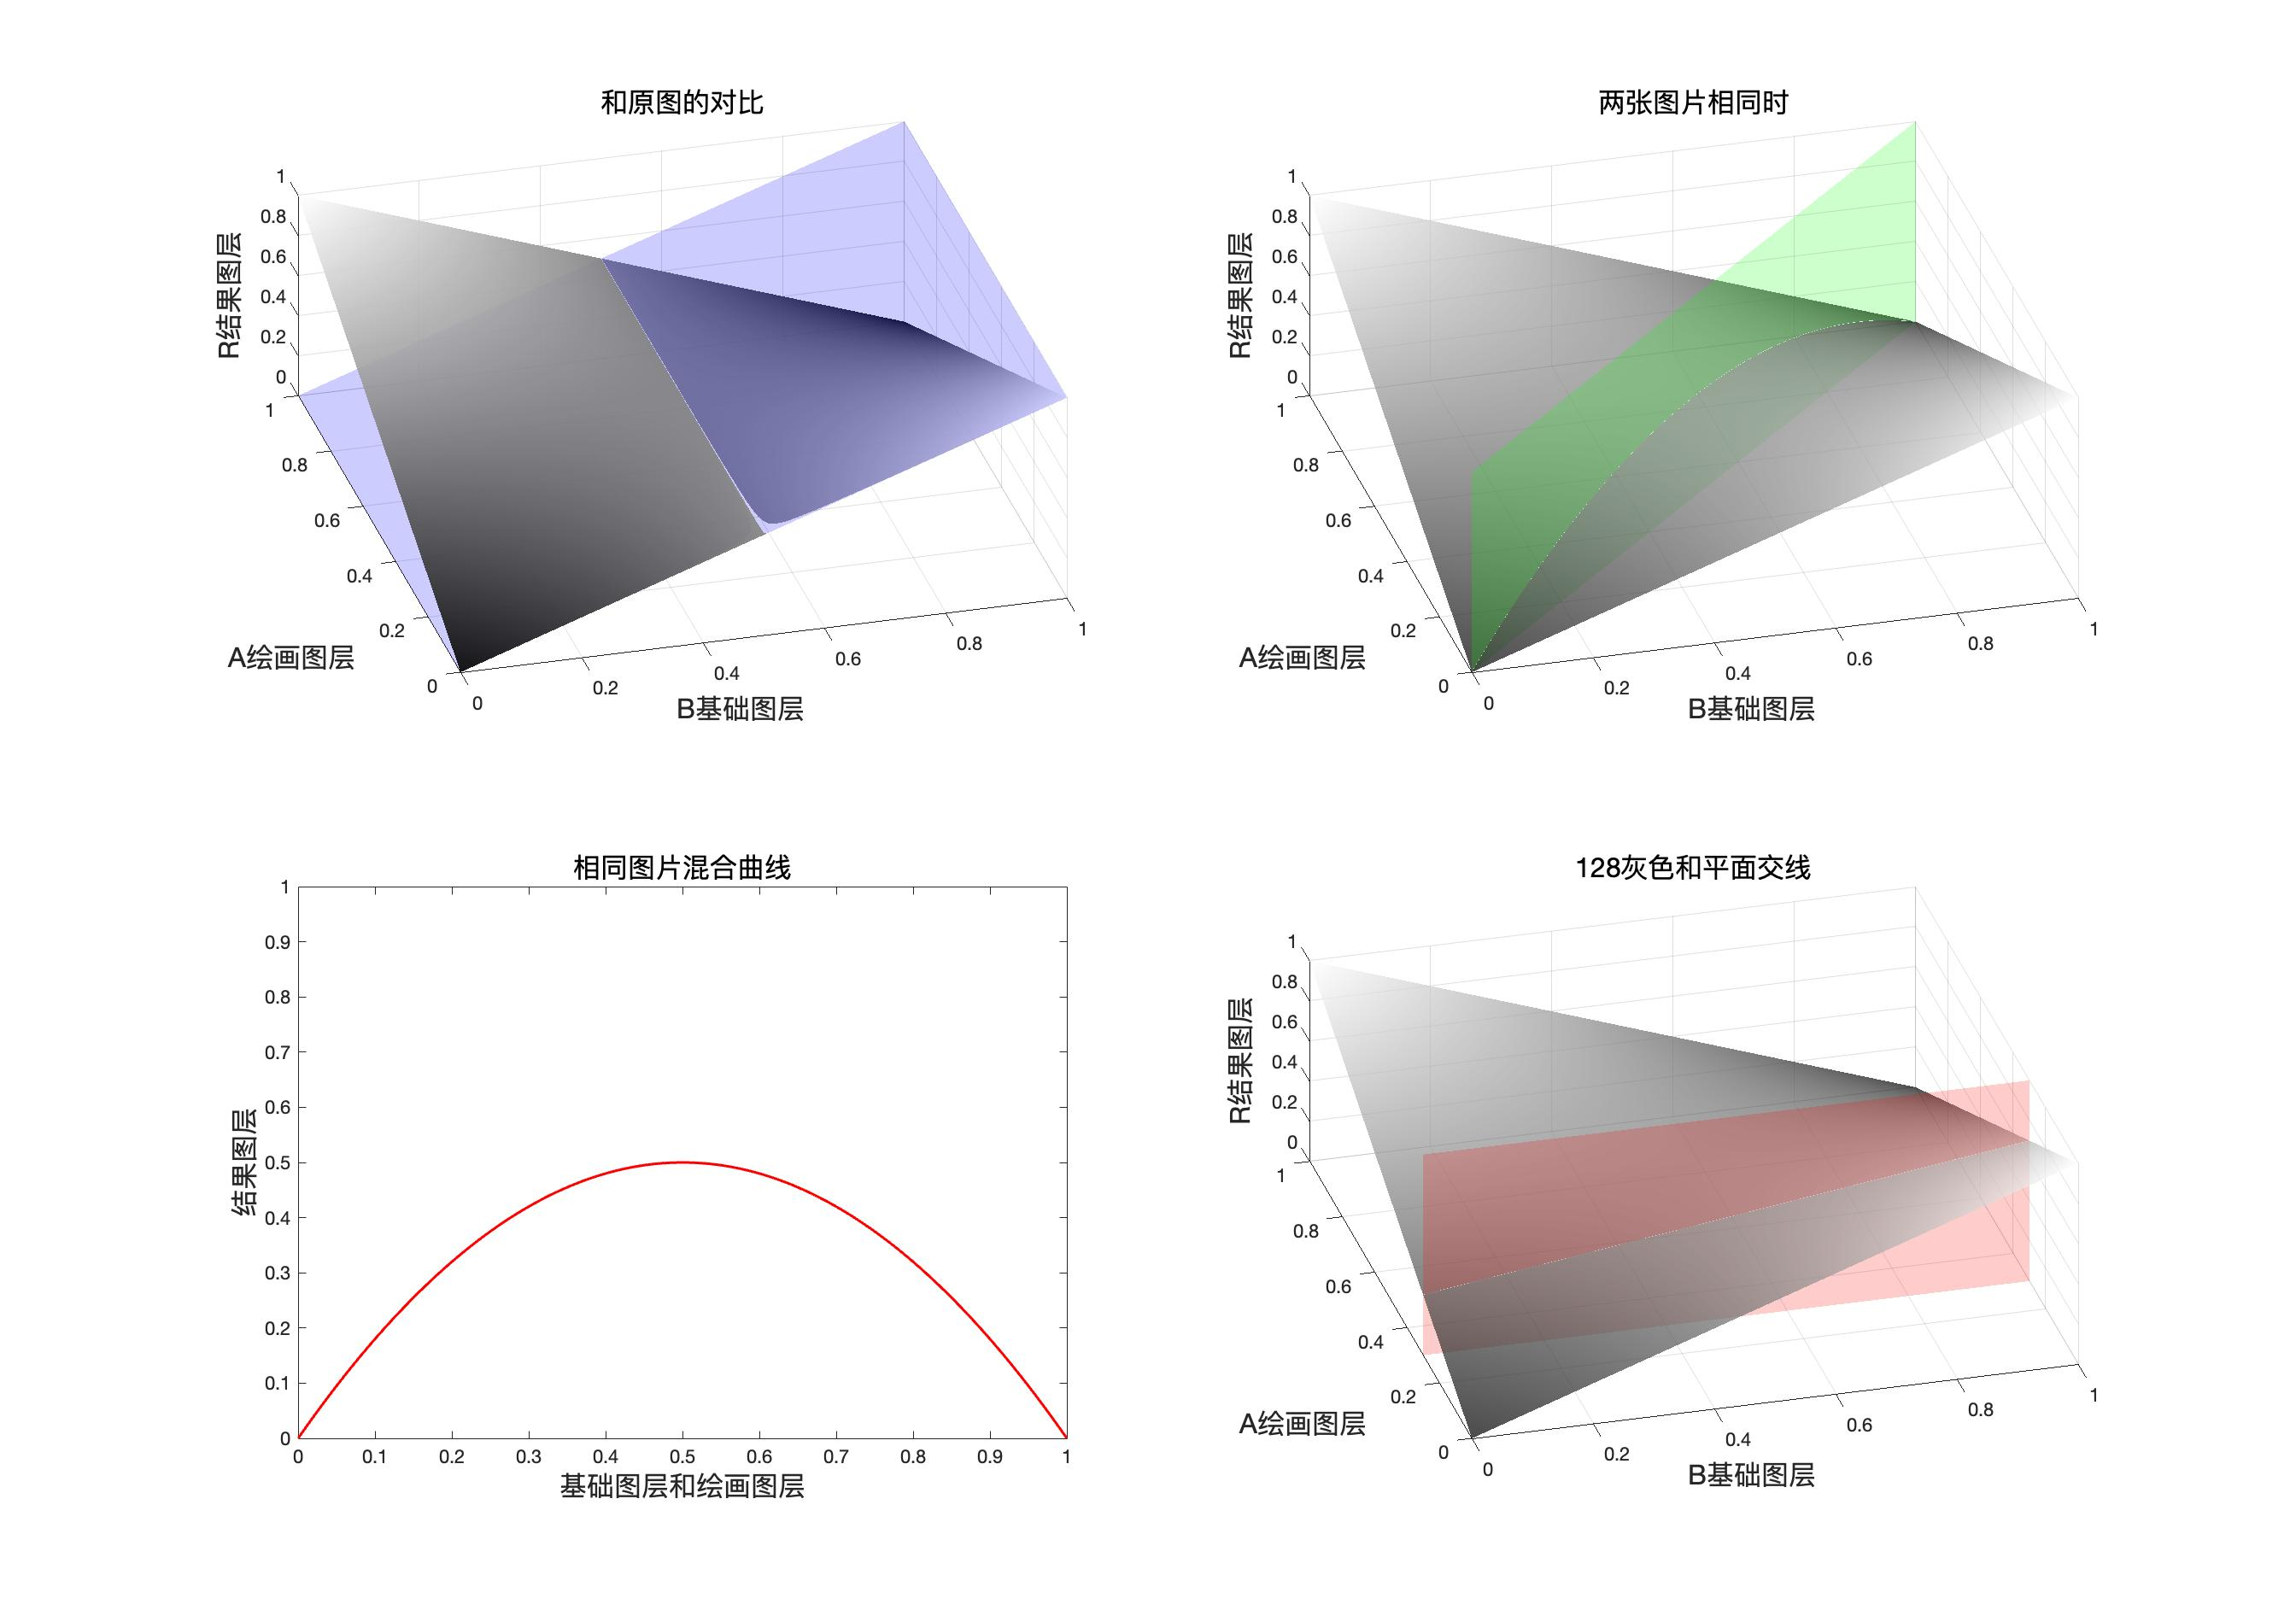
\includegraphics[width=\linewidth]{figure/排除}
	\caption{}
	\label{fig:}
\end{figure}

\subsection{ 程序模拟该模式计算结果}

\begin{lstlisting}
	// 排除
	public static BlendColor Exclusion(BlendColor colorBase, BlendColor colorBlend, double fill, double opacity) {
		double red = ExclusionChannel(colorBase.red.get01Value(), colorBlend.red.get01Value(), fill);
		double green = ExclusionChannel(colorBase.green.get01Value(), colorBlend.green.get01Value(), fill);
		double blue = ExclusionChannel(colorBase.blue.get01Value(), colorBlend.blue.get01Value(), fill);
		return ColorUtils.Opacity(colorBase, new BlendColor(red *255, green* 255, blue * 255), opacity);
	}
	
	private static double ExclusionChannel(double baseValue, double blendValue, double fill) {
		return ColorUtils.round((baseValue + blendValue - 2 * baseValue * blendValue) * fill + (1 - fill) * baseValue,1, 0);
	}
\end{lstlisting}


\begin{result}
\item	排    除(Exclusion)     RGB[113.48,  86.26,  79.82]~ HSY[11.47,  33.66,  93.72 ]~ HSB[ 11.47,  29.66,  44.50]
\end{result}



\subsection{ 验证}
% TODO: \usepackage{graphicx} required
\begin{figure}[h!]
	\centering
	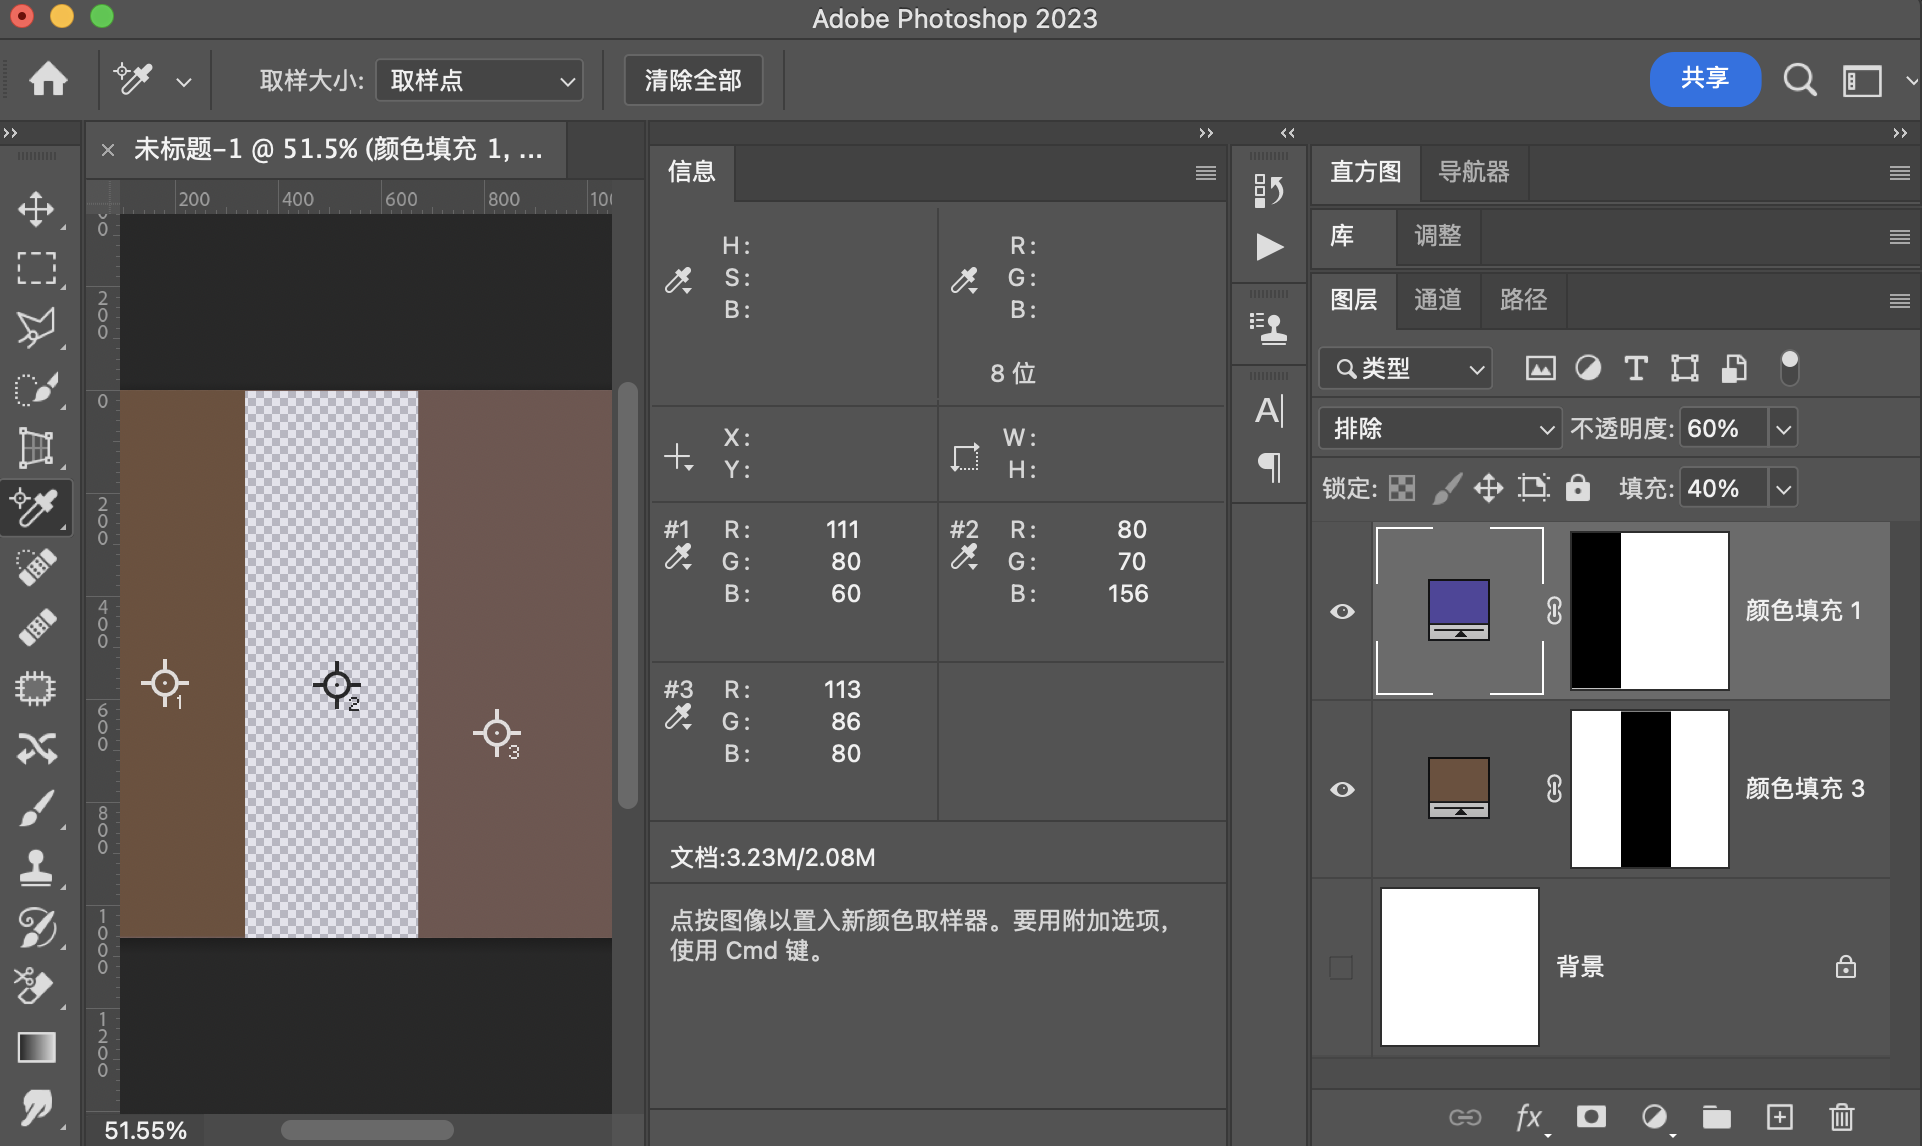
\includegraphics[width=\linewidth]{figure/exclusion}
	\caption{}
	\label{fig:exclusion}
\end{figure}
%
%
%\subsection{ 用途示例}
%
%制作特殊光效,比如人物肖像
\newpage
\section{ 减去Subtract}

\subsection{ 公式}

\begin{equation}r=Subtract(b,a)= b-a\end{equation}

\subsection{ 结合填充}

\begin{equation}r=Fill(b,a)=round(ba)\times fill + (1-fill)\times b\end{equation}

\subsection{ 融合不透明度}

\begin{equation}r=Opacity(b,a)=op\times Fill(b,a)+(1-op)\times b\end{equation}

\subsection{ 映射面和同图等效曲线}
% TODO: \usepackage{graphicx} required
\begin{figure}[h!]
	\centering
	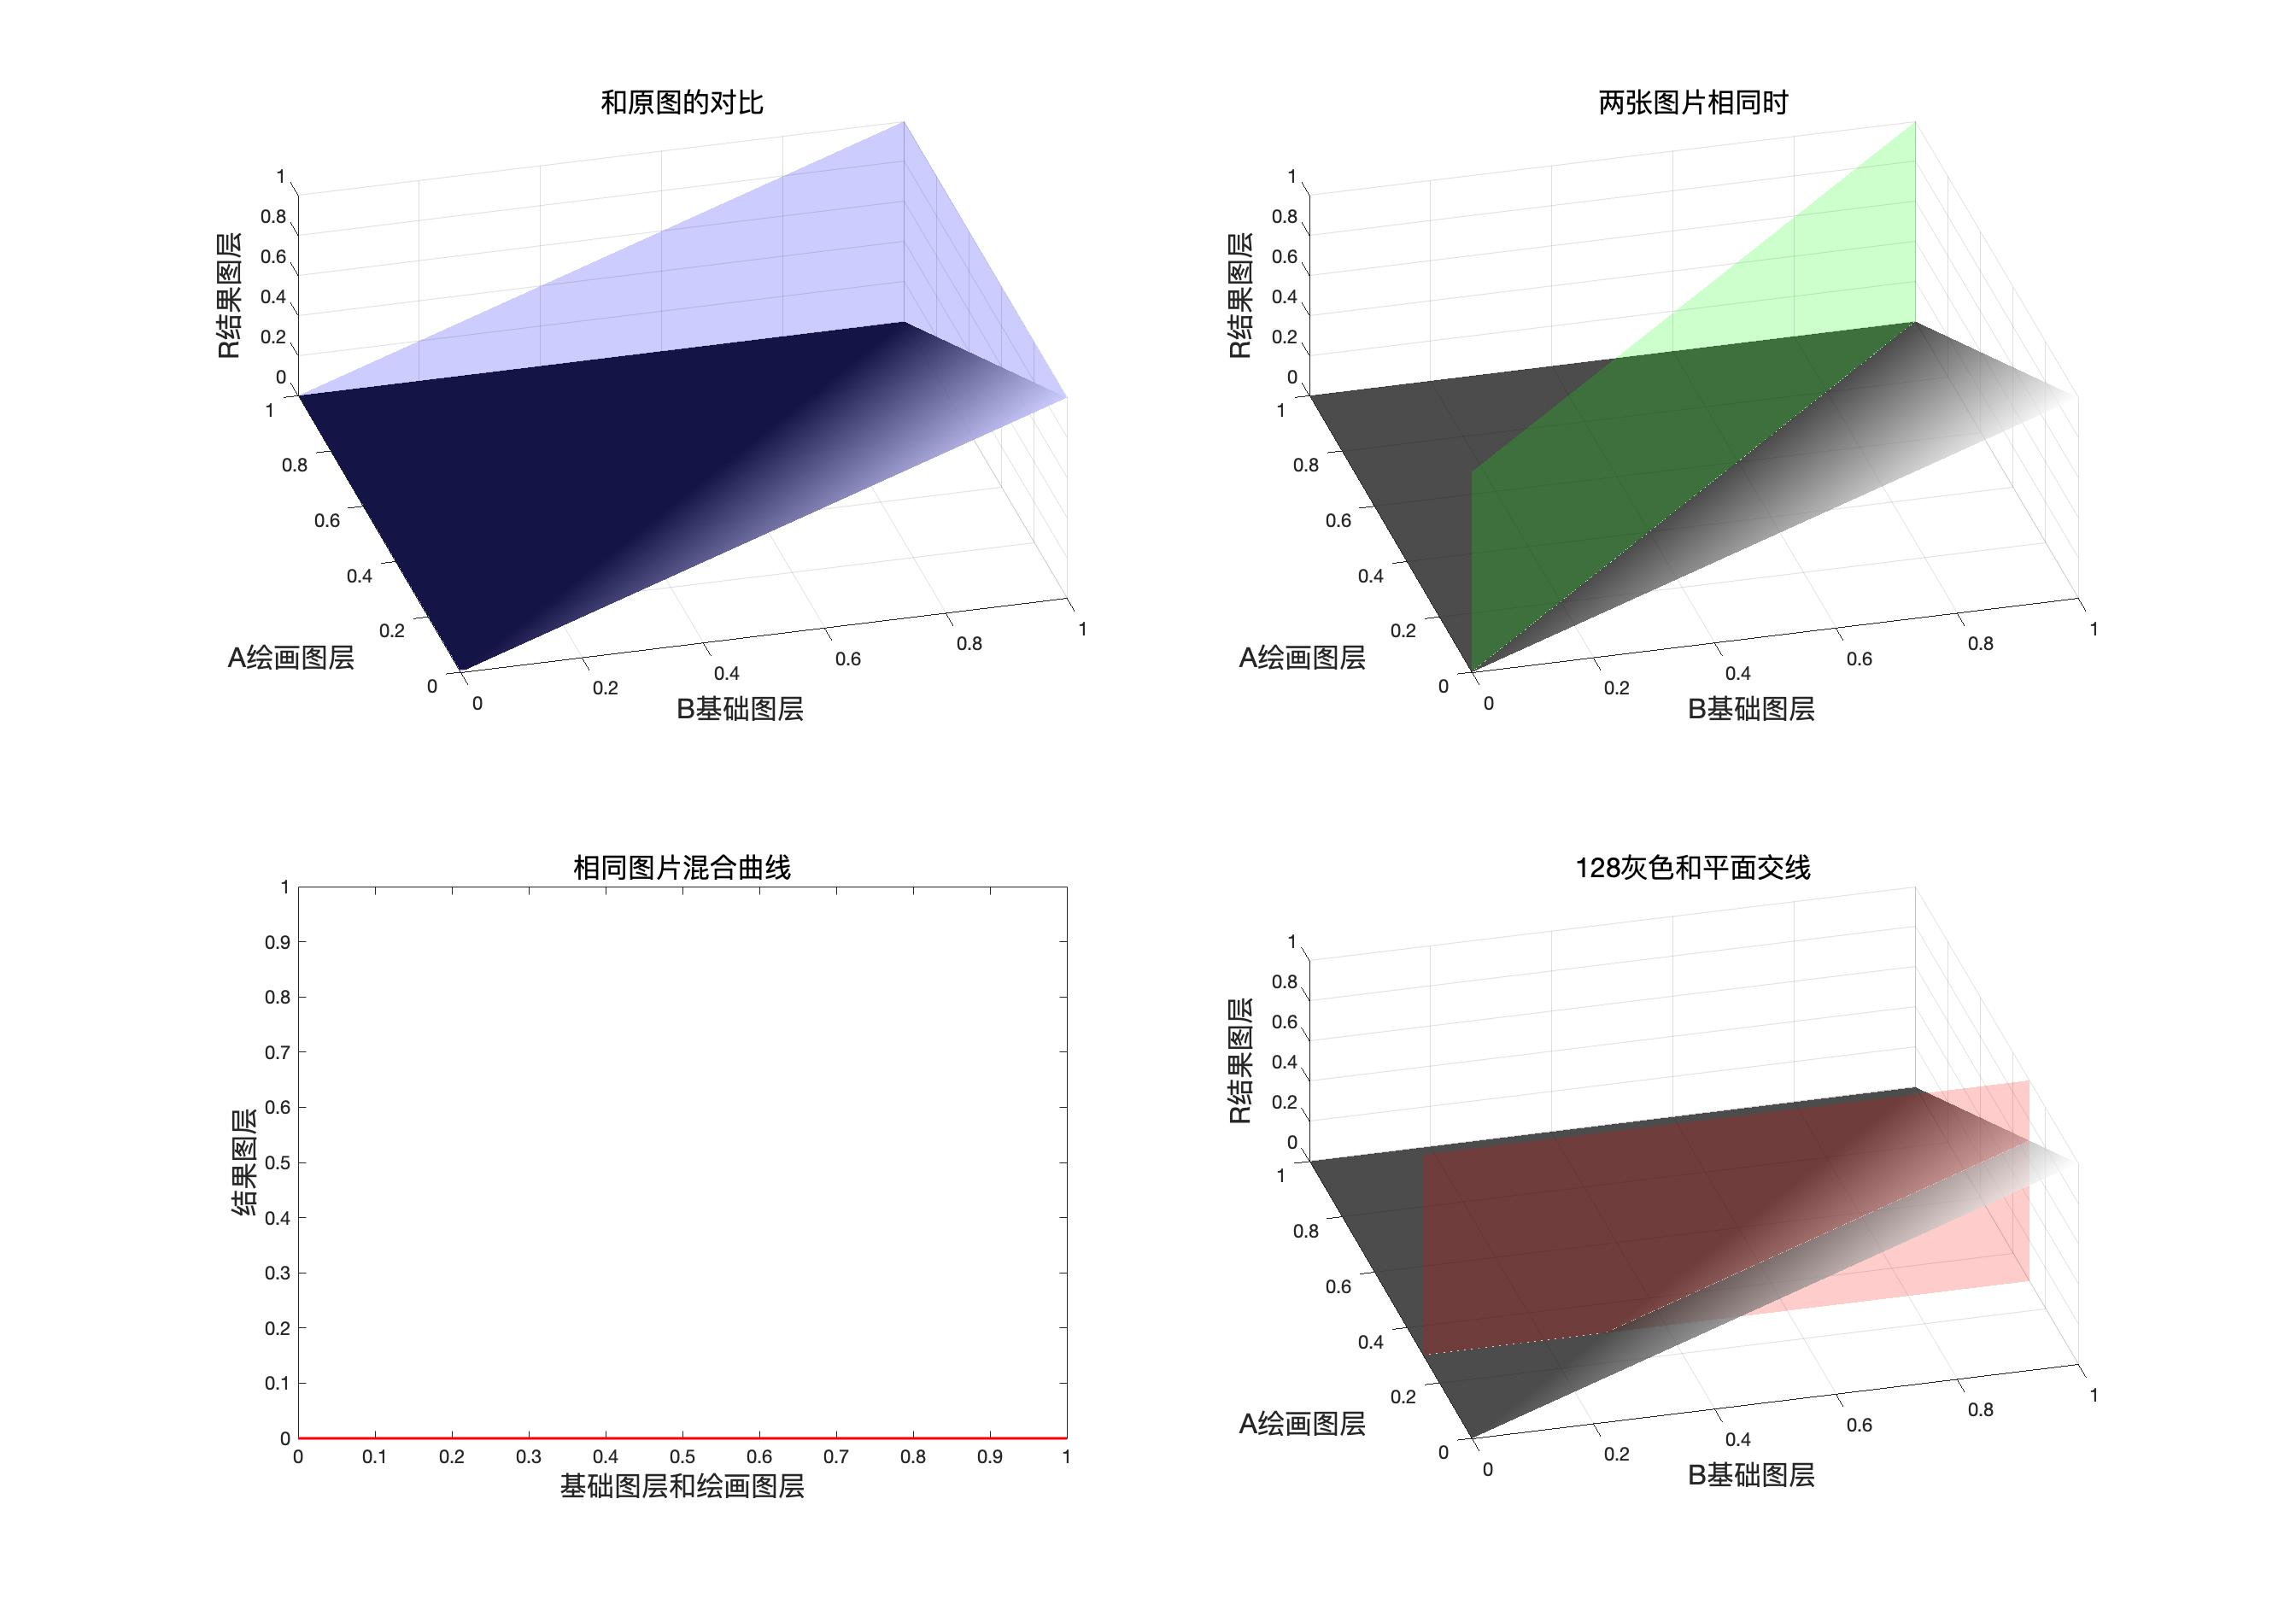
\includegraphics[width=\linewidth]{figure/减去}
	\caption{}
	\label{fig:}
\end{figure}

\newpage
\subsection{ 程序模拟该模式计算结果}

\begin{lstlisting}
	// 减去
	public static BlendColor Substact(BlendColor colorBase, BlendColor colorBlend, double fill, double opacity) {
		double red = SubstactChannel(colorBase.red.get01Value(), colorBlend.red.get01Value(), fill);
		double green = SubstactChannel(colorBase.green.get01Value(), colorBlend.green.get01Value(), fill);
		double blue = SubstactChannel(colorBase.blue.get01Value(), colorBlend.blue.get01Value(), fill);
		return ColorUtils.Opacity(colorBase, new BlendColor(red *255, green* 255, blue * 255), opacity);
	}
	
	private static double SubstactChannel(double baseValue, double blendValue, double fill) {
		return ColorUtils.round(ColorUtils.round((baseValue  blendValue), 1, 0) *fill + (1 - fill)* baseValue, 1, 0);
	}
\end{lstlisting}


\begin{result}
\item 	减    去(Substact)      RGB[ 91.80,  63.20,  45.60]~ HSY[22.86,  46.20,  69.84 ]~ HSB[ 22.86,  50.33,  36.00]
\end{result}



\subsection{ 验证}
% TODO: \usepackage{graphicx} required
\begin{figure}[h!]
	\centering
	\includegraphics[width=\linewidth]{figure/substract}
	\caption{}
	\label{fig:substract}
\end{figure}

%\subsection{用途示例}
%
%制作线稿效果
\newpage
\section{ 划分Divide}

\subsection{ 公式}

\begin{equation}r=Divide(b,a)= \dfrac{b}{a}\end{equation}

\subsection{ 结合填充}

\begin{equation}r=Fill(b,a)= \dfrac{b}{a}\times fill + (1-fill)\times b\end{equation}

\subsection{ 融合不透明度}

\begin{equation}r=Opacity(b,a)=op\times Fill(b,a)+(1-op)\times b\end{equation}

划分和颜色减淡可以通过一次负片操作转换

\subsection{ 一次负片转颜色减淡}

\begin{equation}r=Divide(b,1-a)=\dfrac{b}{1-a}=ColorDodge(b,a)\end{equation}

\subsection{ 映射面和同图等效曲线}
% TODO: \usepackage{graphicx} required
\begin{figure}[h!]
	\centering
	\includegraphics[width=\linewidth]{figure/划分}
	\caption{}
	\label{fig:划分}
\end{figure}


\subsection{ 程序模拟该模式计算结果}

\begin{lstlisting}
	// 划分
	public static BlendColor Divide(BlendColor colorBase, BlendColor colorBlend, double fill, double opacity) {
		double red = DivdeChannel(colorBase.red.get01Value(), colorBlend.red.get01Value(), fill);
		double green = DivdeChannel(colorBase.green.get01Value(), colorBlend.green.get01Value(), fill);
		double blue = DivdeChannel(colorBase.blue.get01Value(), colorBlend.blue.get01Value(), fill);
		return ColorUtils.Opacity(colorBase, new BlendColor(red * 255, green * 255, blue * 255), opacity);
	}
	
	private static double DivdeChannel(double baseValue, double blendValue, double fill) {
		return ColorUtils.round(Math.min(1, baseValue / blendValue) * fill + (1 - fill) * baseValue, 1, 0);
	}
\end{lstlisting}


\begin{result}
\item 划    分(Divide)        RGB[145.56, 122.00,  69.14]~ HSY[41.50,  76.42, 123.25 ]~ HSB[ 41.50,  52.50,  57.08]
\end{result}

\subsection{ 验证}

% TODO: \usepackage{graphicx} required
\begin{figure}[h!]
	\centering
	\includegraphics[width=\linewidth]{figure/divide}
	\caption{}
	\label{fig:divide}
\end{figure}
%
%\subsection{ 用途示例}
%
%颜色矫正

\chapter{颜色组}
\begin{introduction}
\item 这一组和其他都不同,这一组是基于HSY颜色空间,并且设计的计算都是方程组。这里我们给出HSY颜色组的计算算法,为的是引出后面的修改明度和修改饱和度算法。
\end{introduction}
\section{RGB$\rightarrow$HSY转换算法}
\begin{algorithm}
	\caption{计算色相}
	\begin{algorithmic}[1] %显示行号,1是每行都显示
		\Require  颜色$C$
		\Ensure 色相$hue$
		\Function {$Hue$}{$C$}
		\State $min = Min(C_{red},C_{green},C_{blue})$ 
		\State$max = Max(C_{red},C_{green},C_{blue})$
		\State $hue=\left\{ \begin{aligned}&0& \space  max = min \\&60^{\circ}\times \dfrac{C_{green}-C_{blue}}{max-min} &  \space C_{red}=max\quad  \text{且}  \quad C_{green} \geq C_{blue}\\&60^{\circ}\times \dfrac{C_{green}-C_{blue}}{max-min} +360^{\circ}&  \space C_{red}=max\quad \text{且} \quad C_{green}<C_{blue}\\&60^{\circ}\times \dfrac{C_{blue}-C_{red}}{max-min} +120^{\circ}&  \space C_{green}=max\\&60^{\circ}\times \dfrac{C_{red}-C_{green}}{max-min} +240^{\circ}&   \space C_{blue}=max\\\end{aligned}\right. $
		\State \Return $hue$
		\EndFunction
	\end{algorithmic}
\end{algorithm}
\begin{lstlisting}
	public double getHue() {
		ColorItem max = this.getMax();
		ColorItem mid = this.getMid();
		ColorItem min = this.getMin();
		if (Double.doubleToLongBits(max.value) == Double.doubleToLongBits(min.value)) {
			return 0;}
		double hueAbs = (mid.value - min.value) / (max.value - min.value);
		if (max.name == "red") {
			if (this.green.value > this.blue.value) {
				return 60 *hueAbs;
			} else {
				return -60* hueAbs + 360;
			}
		}
		if (max.name == "green") {
			return 60 *hueAbs + 120;}
		if (max.name == "blue") {
			return 60* hueAbs + 240;}
		return 0;
	}
\end{lstlisting}
\begin{algorithm}
	\caption{计算明度}
	\begin{algorithmic}[1] %显示行号,1是每行都显示
		\Require  颜色$C$
		\Ensure 明度$lum$
		\Function {$Lum$}{$C$}
		\State $lum=0.3\times C_{red}+0.59\times C_{green} + 0.11\times C_{blue}$
		\State \Return $lum$
		\EndFunction
	\end{algorithmic}
\end{algorithm}

\begin{lstlisting}
	public double getLum() {
		double lum = 0.3 * this.red.value + 0.59 * this.green.value + 0.11 * this.blue.value;
		return lum;
	}
\end{lstlisting}

\begin{algorithm}
	\caption{计算饱和度}
\begin{algorithmic}[1] %显示行号,1是每行都显示
	\Require  颜色$C$
	\Ensure 饱和度$sat$
	\Function {$Sat$}{$C$}
	\State $min = Min(C_{red},C_{green},C_{blue})$ 
	\State$max = Max(C_{red},C_{green},C_{blue})$
	\State $sat=max-min$
	\State \Return $sat$
	\EndFunction
\end{algorithmic}
\end{algorithm}
\begin{lstlisting}
	public double getSat() {
		double max = this.getMax().value;
		double min = this.getMin().value;
		return max - min;
	}
\end{lstlisting}
\newpage 
\section{HSY替换算法}


\begin{algorithm}
	\caption{改变明度}
	\begin{algorithmic}[1] %显示行号,1是每行都显示
		\Require  颜色$C$,需要改成的明度$lum$
		\Ensure 新的颜色值$C$
		\Function {$SetLum$}{$C, lum$}
		\State $d=lum - Lum(C)$
		\State $C_{red}=C_{red}+d$
		\State  $C_{green}=C_{green}+d$
		\State $C_{blue}=C_{blue}+d$
		\State \Return $ClipColor(C)$
		\EndFunction
	\end{algorithmic}
\end{algorithm}
\begin{lstlisting}
	public static BlendColor setLum(BlendColor color, double lum) {
		double lum2 = color.getLum();
		double temp = lum - lum2;
		double red = color.red.value + temp;
		double green = color.green.value + temp;
		double blue = color.blue.value + temp;
		BlendColor retColor = new BlendColor(red, green, blue);
		return ClipColor(retColor);
	}
\end{lstlisting}
\begin{algorithm}
	\caption{改变饱和度}
	\begin{algorithmic}[1] %显示行号,1是每行都显示
		\Require  颜色$C$,需要改成的饱和度值$sat$
		\Ensure 新的颜色值$C$
		\Function {$SetSat$}{$C, sat$}
		\If{$C_{max}>C_{min}$} % If 语句,需要和EndIf对应
		\State $C_{mid}=\dfrac{(C_{mid}-C_{min})\times sat}{C_{max}-C_{min}}$
		\State $C_{max}=sat$
		\Else
		\State $C_{mid}=C_{max}=0$
		\EndIf
		\State $C_{min}=0$
		\State \Return $C$
		\EndFunction
	\end{algorithmic}
\end{algorithm}
\begin{lstlisting}
	public static BlendColor setSat(BlendColor color, double sat) {
		if (color.getMax().value > color.getMin().value) {
			color.getMid().value = (color.getMid().value - color.getMin().value) * sat
			/ (color.getMax().value - color.getMin().value);
			color.getMax().value = sat;
		} else {
			color.getMid().value = color.getMax().value = 0.0;
		}
		color.getMin().value = 0;
		return color;
	}
\end{lstlisting}
\newpage
\begin{notice}
	\item 这里用了取巧的做法,只涉及饱和度和明度的改变,因为改变色相相当于直接同时改变饱和度和明度。所以不需要替换色相的算法。
\end{notice}
 
\begin{algorithm}
	\caption{矫正颜色}
	\begin{algorithmic}[1] %显示行号,1是每行都显示
		\Require  颜色$C$
		\Ensure 矫正后的颜色$C$
		\Function {$ClipColor$}{$C$}
		\State $lum= Lum(C)$
		\State $min = Min(C_{red},C_{green},C_{blue})$ 
		\State$max = Max(C_{red},C_{green},C_{blue})$
		\If{$min<0$}
		\State$C_{red}=lum+\dfrac{(C_{red}-lum)\times lum}{lum-min}$
		\State$C_{green}=lum+\dfrac{(C_{green}-lum)\times lum}{lum-min}$
		\State$C_{blue}=lum+\dfrac{(C_{blue}-lum)\times lum}{lum-min}$
		\EndIf
		\If{$max>1$}
		\State$C_{red}=lum+\dfrac{(C_{red}-lum)\times (1-lum)}{max-lum}$
		\State$C_{green}=lum+\dfrac{(C_{green}-lum)\times  (1-lum)}{max-lum}$
		\State$C_{blue}=lum+\dfrac{(C_{blue}-lum)\times  (1-lum)}{max-lum}$
		\EndIf
		\State \Return $C$
		\EndFunction
	\end{algorithmic}
\end{algorithm}
\begin{lstlisting}
	 public static BlendColor ClipColor(BlendColor color) {
		double l = color.getLum();
		double min = color.getMin().value;
		if (min < 0.0) {
			double red = l + ((color.red.value - l) * l / (l - min));
			double green = l + ((color.green.value - l) * l / (l - min));
			double blue = l + ((color.blue.value - l) * l / (l - min));
			BlendColor retColor = new BlendColor(red, green, blue);
			return retColor;
		}
		double max = color.getMax().value;
		if (max > 255.0) {
			double red = l + ((color.red.value - l) * (1 - l) / (max - l));
			double green = l + ((color.green.value - l) * (1 - l) / (max - l));
			double blue = l + ((color.blue.value - l) * (1 - l) / (max - l));
			BlendColor retColor = new BlendColor(red, green, blue);
			return retColor;
		}
		return color;
	}
\end{lstlisting}
\newpage
\section{ 色相Hue}


计算方法是基于这个公式
\begin{equation}(H_r,S_r,Y_r)=Hue((H_a,S_a,Y_a),(H_b,S_b,Y_b))=(H_a,S_b,Y_b)\end{equation}

算出HSY的值之后再把HSY转化为RGB的数值。

此时我们想修改基础图层的色相,但是我们只有修改饱和度和明度的公式,于是我们直接对混合图层使用设置饱和度和明度于是我们得到
\begin{equation}Hue(C_b,C_a)=SetLum(SetSat(C_a,Sat(C_b)),Lum(C_b))\end{equation}

\subsection{ 结合填充}

\begin{equation}r=Fill(C_b,C_a)= Hue(C_b,C_a) \times fill + (1-fill)\times C_b\end{equation}

\subsection{ 融合不透明度}

\begin{equation}r=Opacity(C_b,C_a)=op\times Fill(C_b,C_a)+(1-op)\times C_b\end{equation}
\subsection{ 程序模拟该模式计算结果}

\begin{lstlisting}
	// 色相模式
	public static BlendColor HUE(BlendColor colorBase, BlendColor colorBlend, double fill, double opacity) {
		BlendColor temp = HUE_Sub(colorBase, colorBlend);
		double red = temp.red.get01Value() * fill + colorBase.red.get01Value() * (1 - fill);
		double green = temp.green.get01Value() * fill + colorBase.green.get01Value() * (1 - fill);
		double blue = temp.blue.get01Value() * fill + colorBase.blue.get01Value() * (1 - fill);
		return ColorUtils.Opacity(colorBase, new BlendColor(red * 255, green * 255, blue * 255), opacity);
	}
	private static BlendColor HUE_Sub(BlendColor colorBase, BlendColor colorBlend) {
		return ColorUtils.setLum(ColorUtils.setSat(colorBlend, colorBase.getSat()), colorBase.getLum());
	}
\end{lstlisting}
\begin{result}
	\item  色    相(hue)           RGB[104.91,  79.93,  76.97]~ HSY[6.36,  27.94,  87.10  ]~ HSB[  6.36,  26.63,  41.14]
\end{result}
\subsection{ 验证}
% TODO: \usepackage{graphicx} required
\begin{figure}[h!]
	\centering
	\includegraphics[width=\linewidth]{figure/hue}
	\caption{}
	\label{fig:hue}
\end{figure}
%\subsection{ 用途示例}
\newpage
\section{ 饱和度Saturation}
\subsection{ 公式}
计算方法是基于这个公式
\begin{equation}(H_r,S_r,Y_r)= Saturation((H_a,S_a,Y_a),(H_b,S_b,Y_b))=(H_b,S_a,Y_b)\end{equation}

设置饱和度,就直接对基础图层使用设置饱和度
\begin{equation}Saturation(C_b,C_a)=SetLum(SetSat(C_b,Sat(C_s)),Lum(C_b))\end{equation}

\subsection{ 结合填充}

\begin{equation}r=Fill(C_b,C_a)= Saturation(C_b,C_a)\times fill + (1-fill)\times C_b\end{equation}

\subsection{ 融合不透明度}

\begin{equation}r=Opacity(C_b,C_a)=op\times Fill(C_b,C_a)+(1-op)\times C_b\end{equation}

\subsection{ 程序模拟该模式计算结果}

\begin{lstlisting}
	// 饱和度模式
	public static BlendColor Saturation(BlendColor colorBase, BlendColor colorBlend, double fill, double opacity) {
		double redbase = colorBase.red.get01Value();
		double greenbase = colorBase.green.get01Value();
		double bluebase = colorBase.blue.get01Value();
		BlendColor temp = Saturation_Sub(colorBase, colorBlend);
		double red = temp.red.get01Value() * fill + redbase * (1 - fill);
		double green = temp.green.get01Value() * fill + greenbase * (1 - fill);
		double blue = temp.blue.get01Value() * fill + bluebase * (1 - fill);
		return ColorUtils.Opacity(new BlendColor(redbase * 255, greenbase * 255, bluebase * 255),
		new BlendColor(red * 255, green * 255, blue * 255), opacity);
	}
	
	private static BlendColor Saturation_Sub(BlendColor colorBase, BlendColor colorBlend) {
		double sat = colorBlend.getSat();
		double lum = colorBase.getLum();
		return ColorUtils.setLum(ColorUtils.setSat(colorBase, sat), lum);
	}
\end{lstlisting}


\begin{result}
\item 饱 和 度(Saturation)    RGB[114.94,  78.83,  55.54]~ HSY[23.53,  59.40,  87.10 ]~ HSB[ 23.53,  51.68,  45.07]
\end{result}
\newpage
\subsection{ 验证}
% TODO: \usepackage{graphicx} required
\begin{figure}[h!]
	\centering
	\includegraphics[width=\linewidth]{figure/saturation}
	\caption{}
	\label{fig:saturation}
\end{figure}

%
%\subsection{ 用途示例}
%
%颜色匹配

\newpage
\section{ 颜色Color}
%\text{绘画图层}
计算方法是基于这个公式
\begin{equation}(H_r,S_r,Y_r)= Color((H_a,S_a,Y_a),(H_b,S_b,Y_b))=(H_a,S_a,Y_b)\end{equation}

直接对混合图层使用设置明度,则可以得到需要的等效结果
\begin{equation}Color(C_b,C_a)=SetLum(C_a,Lum(C_b))\end{equation}

\subsection{ 结合填充}

\begin{equation}r=Fill(C_b,C_a)= Saturation(C_b,C_a) fill + (1-fill)\times C_b\end{equation}

\subsection{ 融合不透明度}

\begin{equation}r=Opacity(C_b,C_a)=op\times Fill(C_b,C_a)+(1-op)\times C_b\end{equation}

\subsection{ 程序模拟该模式计算结果}

\begin{lstlisting}
	// 颜色模式
	public static BlendColor BlendColor(BlendColor colorBase, BlendColor colorBlend, double fill, double opacity) {
		BlendColor temp = Color_Sub(colorBase, colorBlend);
		double red = temp.red.get01Value() * fill + colorBase.red.get01Value() * (1 - fill);
		double green = temp.green.get01Value() * fill + colorBase.green.get01Value() * (1 - fill);
		double blue = temp.blue.get01Value() * fill + colorBase.blue.get01Value() * (1 - fill);
		return ColorUtils.Opacity(colorBase, new BlendColor(red * 255, green * 255, blue * 255), opacity);
	}
	
	private static BlendColor Color_Sub(BlendColor colorBase, BlendColor colorBlend) {
		return ColorUtils.setLum(colorBlend, colorBase.getLum());
	}
\end{lstlisting}



\begin{result}
\item 颜    色(BlendColor)    RGB[104.67,  78.71,  84.15]~ HSY[347.43,  25.96,  87.10]~ HSB[347.43,  24.80,  41.05]
\end{result}
\newpage
\subsection{ 验证}
% TODO: \usepackage{graphicx} required
\begin{figure}[h!]
	\centering
	\includegraphics[width=\linewidth]{figure/color}
	\caption{}
	\label{fig:color}
\end{figure}


%\subsection{ 用途示例}

\newpage

\section{ 明度Luminosity}

计算方法是基于这个公式
\begin{equation}(H_r,S_r,Y_r)= Luminosity((H_a,S_a,Y_a),(H_b,S_b,Y_b))=(H_b,S_b,Y_a)\end{equation}

\subsection{ 设置明度,就直接使用设置明度}

\begin{equation}Luminosity(C_b,C_a)=SetLum(C_b,Lum(C_a))\end{equation}

\subsection{ 结合填充}

\begin{equation}r=Fill(C_b,C_a)= Luminosity(C_b,C_a) \times fill + (1-fill)\times C_b\end{equation}

\subsection{ 融合不透明度}

\begin{equation}r=Opacity(C_b,C_a)=op\times Fill(C_b,C_a)+(1-op)\times C_b\end{equation}

\subsection{ 程序模拟该模式计算结果}

\begin{lstlisting}
	// 明度模式
	public static BlendColor Luminosity(BlendColor colorBase, BlendColor colorBlend, double fill, double opacity) {
		BlendColor temp = Luminosity_Sub(colorBase, colorBlend);
		double red = temp.red.get01Value() *fill + colorBase.red.get01Value()* (1 - fill);
		double green = temp.green.get01Value() *fill + colorBase.green.get01Value()* (1 - fill);
		double blue = temp.blue.get01Value() *fill + colorBase.blue.get01Value()* (1 - fill);
		return ColorUtils.Opacity(colorBase, new BlendColor(red *255, green* 255, blue * 255), opacity);
	}
	
	private static BlendColor Luminosity_Sub(BlendColor colorBase, BlendColor colorBlend) {
		return ColorUtils.setLum(colorBase, colorBlend.getLum());
	}
\end{lstlisting}
\begin{result}
\item 明    度(Luminosity)    RGB[109.89,  78.89,  58.89]~ HSY[23.53,  51.00,  85.99 ]~ HSB[ 23.53,  46.41,  43.09]
\end{result}
\newpage
\subsection{ 验证}
% TODO: \usepackage{graphicx} required
\begin{figure}[h!]
	\centering
	\includegraphics[width=\linewidth]{figure/lum}
	\caption{}
	\label{fig:lum}
\end{figure}
%\subsection{ 用途示例}
%和黑白调整图层配合,可以实现一些特殊效果。
\newpage
\chapter{特殊的5种模式}
\section{ 穿透}
穿透会出现在建立分组的时候,如果选择穿透,则此时效果和不建分组一样,但是如果修改为正常或者其他模式,则会先把这一组的图层计算出结果,然后用结果作为混合图层和下方图层进行运算。
\section{ 相加}
相加在计算和应用图像中,此时相当于强化的线性减淡,公式为
\begin{equation}Add(b,a)= \dfrac{b+a}{zoom}+offect\end{equation}
缩放$zoom$的取值范围是$[1,2]$
补偿值$offect$的取值范围是$[0,255]$
\section{ 相减}
相减在计算和应用图像中,此时相当于强化的减去,公式为
\begin{equation}Subtract(b,a)= \dfrac{b-a}{zoom}+offect\end{equation}
缩放$zoom$的取值范围是$[1,2]$
补偿值$offect$的取值范围是$[0,255]$
\section{ 背后}
背后模式简单来说就是,有像素点则笔刷或油漆桶工具不能修改,没有像素点的透明像素可以被修改。
\section{ 擦除}
功能相当于橡皮擦
\newpage 
\chapter{调整图层和图层混合模式}
如果调整图层和混合图层混用会发生什么
我们假设调整图层为$Adjustment(Layer)$,
则对于像素点$Adjustment(pix)$,
对于通道$Adjustment(channel)$
则结果公式可以写作
$$r=BlendMode(b,Adjustment(b))$$
也就是说相当于,先使用调整图层产生基础图层调整之后的图层,再使用调整后的图层和原先的基础图层进行图层混合模式的操作。
此处我们以曲线调整图层为例
如果我们对原图层新建调整图层,并且对调整图层使用图层混合模式,如图\ref{fig:adjustandblend1}所示。
\begin{figure}[h!]
	\centering
	\includegraphics[width=\linewidth]{figure/adjustandblend1}
	\caption{}
	\label{fig:adjustandblend1}
\end{figure}
\newpage 
如果是正常模式,则相当于原图,但是只要我们选择一个别的模式,或拉一下曲线,结果就会不同。如图\ref{fig:adjustandblend2}所示。
\begin{figure}[h!]
	\centering
	\includegraphics[width=\linewidth]{figure/adjustandblend2}
	\caption{}
	\label{fig:adjustandblend2}
\end{figure}


\newpage 

我们可以看到在不拉曲线的前提下,结果和直接用原图做正片叠底是一样的。
如图\ref{fig:adjustandblend3}所示。
\begin{figure}[h!]
	\centering
	\includegraphics[width=\linewidth]{figure/adjustandblend3}
	\caption{}
	\label{fig:adjustandblend3}
\end{figure}

\chapter{工具和混合模式}
\begin{introduction}
	\item 在PS中,不止是图层可以选择图层混合模式,有一些工具也可以使用图层混合模式,不同的是,这些都是直接修改原图层,相当于,新建空白图层,再在空白图层上产生新的像素,并且此空白图层作为混合图层。换句话说,图层的混合模式是非破坏性的,工具的混合模式是破坏性的。
\end{introduction}
\section{画笔类}
\subsection{画笔工具}
画笔工具是最典型的破坏性编辑工具,因为它就像画笔在纸上写字一样,但是,这样操作的本质是新建一个透明图层,在透明图层上面使用画笔绘画,再将当前绘画的图层作为基础图层,带有画笔痕迹的图层作为绘画图层,再进行混合模式的运算。和直接使用透明图层不同的是,结果图层就是基础图层,或者说,PS将运算过程隐藏了。

\newpage
\subsection{铅笔工具}
\newpage
\subsection{历史记录画笔工具}
\newpage
\subsection{历史记录艺术画笔工具}
\newpage
\subsection{修复画笔工具}
\newpage
\subsection{污点修复画笔工具}
\newpage
\subsection{颜色替换工具}
\newpage
\section{油漆桶工具}
\newpage
\section{图章类}
\newpage
\subsection{仿制图章}
\newpage
\subsection{图案图章工具}
\newpage
\section{渐变工具}
\newpage 
\section{计算类}
\newpage
\subsection{应用图像}
\newpage
\subsection{计算}
\newpage
\section{其他}
\newpage
\subsection{锐化工具}
\newpage
\subsection{模糊工具}
\newpage
\subsection{涂抹工具}
\newpage
\chapter{图层样式和混合模式}
\section{斜面和浮雕}
\newpage
\section{描边}
\newpage
\section{内阴影}
\newpage
\section{内发光}
\newpage
\section{光泽}
\newpage
\section{颜色叠加}
\newpage
\section{渐变叠加}
\newpage
\section{图案叠加}
\newpage
\section{外发光}
\newpage
\section{投影}
\newpage
\section{常规混合}
\subsection{混合模式}
\subsection{不透明度}
\newpage
\section{高级混合}
\subsection{填充不透明度}
\newpage
\subsection{通道}
\newpage
\subsection{挖空}
\newpage
\subsection{将内部效果混成组}
\newpage
\subsection{将剪贴图层混成组}
\newpage
\subsection{透明形状图层}
\newpage
\subsection{图层蒙版隐藏效果}
\newpage
\subsection{矢量蒙版隐藏效果}
\newpage
\chapter{混合颜色带Blend If}
\begin{introduction}
	\item 混合颜色带是我们常用的融图工具
	\item 混合颜色带相当于GIMP中的透明颜色
\end{introduction}
\section{怎么开启}
开启方法,就是双击
\section{原理}
混合颜色带有两个控制带,四个滑块,每个滑块可以分裂为两个小滑块,这些东西看似复杂,但是实际上都控制一件事,就是决定当前图层有哪些像素需要变成透明的。
那么如何决定,决定的方式又是哪些。

上方的控制带决定在两个滑块中间的像素保留,在两个滑块之外的变透明。

下方的控制带决定下方图层像素在两个滑块之外的像素,其上方的像素变透明。

\begin{notice}
\item 简单来说就是,两个控制带都是让本图层的像素点变透明,一个是用本图层的像素来决定,一个是用下方图层的像素来决定。
\end{notice}


\section{色彩模式和颜色混合带}

如果我们要选取某些像素点,首先我们需要知晓当前的图片的色彩空间是什么,如果是RGB,那么选择灰色、红色、绿色、蓝色的表现会有什么不同。

\subsection{RGB}
RGB空间有四个选项,分别是灰色、红色、绿色、蓝色
红色、绿色、蓝色计算方法相同,都是非常直白的使用对应通道的数值来计算。

如果选择的是红色、绿色或蓝色,那么如果滑动上面的滑块,则在就是根据本图层的对应通道值来决定哪些像素透明。
总范围是$[0,255]$,滑块中间的范围是$[50,200]$,那么本图层中,满足通道值属于$[0,50]$
如果滑动下面的滑块(这个是最常见的),则此时我们就是使用
\begin{equation}
gray=0.3\times R+0.59\times G + 0.11\times B
\end{equation}

并且,我们容易得出$gray\in [0,255]$。
所以对于灰色,我们需要按照上面计算一下结果,然后根据这个结果在$[0,255]$之间的取值进行处理。

\subsection{CMYK}
RGB转CMYK
\begin{equation}
	\begin{aligned}
	&K= 1-Max(r,g,b)\\
	&C= \dfrac{1-r-K}{1-K} \\
	&M= \dfrac{1-g-K}{1-K} \\
	&Y= \dfrac{1-b-K}{1-K} \\
	\end{aligned}
\end{equation}

CMYK 转 RGB

\begin{equation}
	\begin{aligned}
&R= 255 \times (1-C) \times (1-K)\\
&G= 255 \times (1-M) \times (1-K)\\
&B= 255 \times (1-Y) \times (1-K)\\
\end{aligned}
\end{equation}

在得到了RGB数值之后,我们就可以计算出灰色数值
\subsection{LAB}
LAB 色彩空间共有三个维度分别是Lightness,A channel, B channel

\subsection{灰度}
灰度就是将RGB数值计算为灰色,但是这里灰色的计算方式有些许不同,
这里的计算方式是
\begin{equation}
	gray=0.4\times R+0.4\times G + 0.2\times B
\end{equation}

\chapter{速查表}
\begin{table}[htbp]
	\centering
	\caption{ 快捷键和中性色}
	\begin{tabular}{|l|l|c|}
		\hline
		\textbf{\large {名称}}& \textbf{\large{快捷键}} &  \textbf{\large{中性色}}  \\
		\hline
		正常&\keys{CMD/CTRL} + \keys{SHIFT} + \keys{N}&\\
		\hline
		溶解 & &\\
		\hline
		变暗 &\keys{CMD/CTRL} + \keys{SHIFT} + \keys{K} &白\\
		\hline
		正片叠底 &\keys{CMD/CTRL} + \keys{SHIFT} + \keys{M}&白\\
		\hline
		线性加深 &\keys{CMD/CTRL} + \keys{SHIFT} + \keys{A} &白\\
		\hline
		颜色加深 & \keys{CMD/CTRL} + \keys{SHIFT} + \keys{B}&白\\
		\hline
		深色 &&白\\
		\hline
		变亮 & \keys{CMD/CTRL} + \keys{SHIFT} + \keys{G}&黑\\
		\hline
		滤色 & \keys{CMD/CTRL} + \keys{SHIFT} + \keys{S}&黑\\
		\hline
		线性减淡 &\keys{CMD/CTRL} + \keys{SHIFT} + \keys{W}&黑\\
		\hline
		颜色减淡&\keys{CMD/CTRL} + \keys{SHIFT} + \keys{D}&黑\\
		\hline
		浅色&&黑\\
		\hline
		叠加&\keys{CMD/CTRL} + \keys{SHIFT} + \keys{O} &中性灰\\
		\hline
		柔光&\keys{CMD/CTRL} + \keys{SHIFT} + \keys{F}&中性灰\\
		\hline
		强光& \keys{CMD/CTRL} + \keys{SHIFT} + \keys{H}&中性灰\\
		\hline
		点光&\keys{CMD/CTRL} + \keys{SHIFT} + \keys{Z}&中性灰\\
		\hline
		亮光&\keys{CMD/CTRL} + \keys{SHIFT} + \keys{V}&中性灰\\
		\hline
		线性光&\keys{CMD/CTRL} + \keys{SHIFT} + \keys{J}&中性灰\\
		\hline
		实色混合&\keys{CMD/CTRL} + \keys{SHIFT} + \keys{L}&中性灰\\
		\hline
		差值& \keys{CMD/CTRL} + \keys{SHIFT} + \keys{E}&黑\\
		\hline
		排除&\keys{CMD/CTRL} + \keys{SHIFT} + \keys{X}  &黑\\
		\hline
		减去& &黑\\
		\hline
		划分&  &黑\\
		\hline
		色相& \keys{CMD/CTRL} + \keys{SHIFT} + \keys{U} &\\
		\hline
		饱和度& \keys{CMD/CTRL} + \keys{SHIFT} + \keys{T}&\\
		\hline
		颜色&\keys{CMD/CTRL} + \keys{SHIFT} + \keys{C} &\\
		\hline
		明度& \keys{CMD/CTRL} + \keys{SHIFT} + \keys{Y}&\\
		\hline
	\end{tabular}
\end{table}
\begin{table}[htbp]
	\centering
	\caption{ 27种图层混合模式公式汇总}
\begin{tabular}{|l|l|l|}
	\hline
	\textbf{\large {名称}}& \textbf{\large{公式}} &  \textbf{\large{添加填充}}  \\
	\hline
	正常& $a$& $fill\times result+(1-fill)\times b$     \\
	\hline
	溶解 & $a$& $Random_{fill}(b,a)$    \\
	\hline
	变暗 & $Min(b,a)$& $fill\times result+(1-fill)\times b$     \\
	\hline
	正片叠底 &$ b\times a$ & $fill\times result+(1-fill)\times b$    \\
	\hline
	线性加深 & $b-(1-a)$ &  $b-(1-a)\times fill$  \\
	\hline
	颜色加深 & $1-\frac{1-b}{1-(1-a)}$ & $1-\frac{1-b}{1-(1-a)\times fill}$   \\
	\hline
	深色 &$Min(Sum(Pix_b),Sum(Pix_a))$&$fill\times result+(1-fill)\times b$    \\
	\hline
	变亮 &  $Max(b,a)$& $fill\times result+(1-fill)\times b$    \\
	\hline
	滤色 & $1-(1-b)\times (1-a)$ &  $fill\times result+(1-fill)\times b$   \\
	\hline
	线性减淡 &  $b+a$& $b+a\times fill$   \\
	\hline
	颜色减淡&$ \frac{b}{1-a} $&$\frac{b}{1-a\times fill}$    \\
	\hline
	浅色&$Max(Sum(Pix_b),Sum(Pix_a))$&$fill\times result+(1-fill)\times b$    \\
	\hline
	叠加& $\left\{\begin{aligned}2ba&&\text{当} 0\leq b \leq 0.5\\1-2(1-b)(1-a)&&\text{当} 0.5< b \leq 1\\\end{aligned}\right.$ & $fill\times result+(1-fill)\times b$    \\
	\hline
柔光&$\left\{\begin{aligned}&(2a-1)(b^2-b)+b& \text{当}0\leq a \leq 0.5\\&(2a-1)(\sqrt{b}-b)+b&\text{当} 0.5< a \leq 1\end{aligned}\right.$  &$fill\times result+(1-fill)\times b$     \\
	\hline
	强光& $\left\{\begin{aligned}2ba&&\text{当} 0\leq a \leq 0.5\\1-2(1-b)(1-a)&&\text{当} 0.5< a \leq 1\\\end{aligned}\right.$ &$fill\times result+(1-fill)\times b$     \\
	\hline
	点光&$\left\{ \begin{aligned}&Min(b,2a)& \text{当}0\leq a \leq 0.5\\&Max(b,2(a-0.5))&\text{当} 0.5< a \leq 1  \end{aligned}\right.$  & $fill\times result+(1-fill)\times b$    \\
	\hline
	亮光&$\left\{ \begin{aligned}&1-\frac{(1-b)}{2a}&\text{当} 0\leq a \leq 0.5\\&\frac{b}{1-2(a-0.5)}&\text{当} 0.5< a \leq 1\end{aligned}\right.$  &$fill\times result+(1-fill)\times b$    \\
	\hline
	线性光&  $b+2a-1$&$\left\{\begin{aligned}b+2a\times fill-1&&\text{当} 0\leq a \leq 0.5\\b+2a\times fill-1\times fill&&\text{当} 0.5< a \leq 1\\\end{aligned}\right.$    \\
	\hline
	实色混合& $\left\{ \begin{aligned}&1&b+a\geq 1\\&0&else  \end{aligned}\right.$ &  $\left\{ \begin{aligned}&0&  \frac{fill\times a+b-fill}{(1-fill)}<0\\ &\frac{fill\times a+b-fill}{(1-fill)}&0\leq \frac{fill\times a+b-fill}{(1-fill)}\leq 1\\ &1&  \frac{fill\times a+b-fill}{(1-fill)}>1 \end{aligned}\right.$  \\
	\hline
	差值& $|b-a|$ &$|b-a|\times fill$    \\
	\hline
	排除&  $b+a-2ba$&$fill\times result+(1-fill)\times b$     \\
	\hline
	减去& $b-a$ & $fill\times result+(1-fill)\times b$    \\
	\hline
	划分& $\frac{b}{a}$ &$fill\times result+(1-fill)\times b$     \\
	\hline
	色相&  $(H_a,S_b,Y_b) $&$fill\times result+(1-fill)\times b$     \\
	\hline
	饱和度&  $(H_b,S_a,Y_b)$& $fill\times result+(1-fill)\times b$    \\
	\hline
	颜色& $(H_a,S_a,Y_b)$ &  $fill\times result+(1-fill)\times b$   \\
	\hline
	明度& $(H_b,S_b,Y_a)$ &  $fill\times result+(1-fill)\times b$   \\
	\hline
\end{tabular}
\end{table})
\chapter{参考文档}

<http://www.simplefilter.de/en/basics/mixmods.html>

<https://printtechnologies.org/wpcontent/uploads/2020/03/pdfreference1.6addendumblendmodes.pdf>
